%*******************************************************************************************
% File ini merupakan file template LaTEX untuk penulisan Disertasi pada Universitas Gunadarma Tahun 2018
%% Programmer  : Robby Kurniawan Harahap
%% E-mail  : robby_kurniawan@staff.gunadarma.ac.id
%% Pembuatan program template makalah ini dibuat dengan menggunakan :
%% Linux Opensuse Leap 42.3
%% texstudio versi 2.12.22 dan kile
%% TeX Live 2016/TeX Live for SUSE Linux
%% acrobat reader atau okular

%*******************************************************************************************

%berikut langkah-langkah untuk mendapatkan hasil akhir Disertasi
%================================================================
%Untuk pengguna texstudio (Linux dan Windows) :
% buka template, MainTemplateDisertasi.tex
% run compile atau tekan tombol f9 pada keyboard untuk mendapatkan hasil

%Untuk pengguna texmaker (Linux dan Windows):
% buka template, MainTemplateDisertasi.tex
% run compile untuk mendapatkan hasil

%Untuk pengguna kile:
% buka template, MainTemplateDisertasi.tex
% run compile PDFLatex untuk mendapatkan hasil

%berikut ini langkah-langkah untuk mendapatkan hasil akhir disertasi

%==============================================================
% Untuk platform Windows, berikut software yang diperlukan :
% 1. MiKTeX (Latex versi Windows). Dapat didownload dari situs http://miktex.org/
% 2. WinEdt (dapat didownload dari http://www.winedt.com
% 3. ghostscript
% 4. gimp untuk mengedit gambar
% 5. Adobe reader atau foxit reader

%==============================================================
% 
%  berikut ini langkah-langkah untuk mendapatkan hasil akhir disertasi menggunakan  WinEdt :
%  tekan tombol Latex
%  tekan tombol bibtex
%  tekan tombol makeindex
%  tekan tombol Latex
%  tekan tombol Latex
%  tekan tombol Pdf Latex/Pdf Texify
%=======================================================================================================
% jika terjadi masalah dalam penulisan silahkan hubungi programmer 
%% E-mail  : robby_kurniawan@staff.gunadarma.ac.id


\documentclass[a4paper,12pt,oneside]{disertasi}
\usepackage[a4paper,top=3cm,right=3cm,bottom=3cm,left=4cm]{geometry}
\usepackage[indonesia]{babel}
\usepackage[T1]{fontenc}
\usepackage[latin1]{inputenc}
\setcounter{secnumdepth}{3}
\setcounter{tocdepth}{3}
\setcounter{totalnumber}{4}
\usepackage{array}
\usepackage{multirow}
\usepackage{array,longtable}
\usepackage{graphicx}
\usepackage{epstopdf}
\usepackage{setspace}
\usepackage{multind}
\usepackage{rotating} %for rotate/sideway text
\usepackage{subfig} %for make floating sub-figure
\usepackage{natbib}
\usepackage{float}
\usepackage{lscape}
\usepackage{pseudocode}

\usepackage{lipsum}
\usepackage{fancyhdr}
\usepackage{amsmath}
\usepackage{enumerate}
\usepackage{enumitem}
\usepackage[table,xcdraw]{xcolor}
\usepackage{afterpage}
\usepackage{algorithmicx}
\usepackage{algcompatible}
\usepackage{algpseudocode}
\usepackage[
bookmarksopen,
bookmarksdepth=2,
breaklinks=true]{hyperref}
\hypersetup{
	colorlinks=true, % tadinya false
	linkcolor=black,
	citecolor=black,
	filecolor=black,
	%pagecolor=black,
	urlcolor=blue,
	bookmarks=true,
	pdfborder={0 0 0 0},
	pdftitle={MainTemplateDisertasi},
	pdfauthor={me},
	pdfkeywords={somekeywords},
	pdfdisplaydoctitle=true,
	pdftoolbar=true,
	pdfmenubar=true,
	pdfstartview=X Y Z
}
\usepackage{amssymb}% http://ctan.org/pkg/amssymb
\usepackage{pifont}% http://ctan.org/pkg/pifont
\usepackage{listings}
\usepackage{alltt}
%\usepackage[toc,page]{appendix} by sunny
\usepackage{multirow}
\usepackage{booktabs}
\usepackage{tabularx}
\usepackage[table]{xcolor}
\usepackage{longtable}
\hypersetup{breaklinks=true}
\usepackage{tikz}
%\usepackage{adjustbox}

\usepackage[export]{adjustbox}

\usepackage[hyphenbreaks]{breakurl}
\usepackage{etoolbox}
\usepackage{array, hhline}
\usepackage{colortbl}
\usepackage{lmodern}
\usepackage{color} %red, green, blue, yellow, cyan, magenta, black, white
\definecolor{mygreen}{RGB}{28,172,0} % color values Red, Green, Blue
\definecolor{mylilas}{RGB}{170,55,241}
\definecolor{darkblue}{rgb}{0,0,.75}
\usepackage{caption}
\usepackage{adjustbox} % auto adjust table
\usepackage[normalem]{ulem}
\useunder{\uline}{\ul}{}
\usepackage{subcaption}

\usepackage[chapter]{algorithm}
\usepackage{makecell}
\usepackage{graphbox}

%\usepackage[export]{adjustbox}

\usepackage{multicol}
\setlength{\columnsep}{0cm}

\usepackage{titlesec}
\titleformat{\chapter}[display]
{\normalfont\Large\bfseries\centering}{\centering\chaptertitlename\ \thechapter}{14pt}{\Large\bfseries}
\titlespacing*{\chapter}{0pt}{-30pt}{40pt}

\usepackage{textcomp}


\renewcommand{\thechapter}{\Roman{chapter}\bfseries}
\renewcommand{\thesection}{\arabic{chapter}.\arabic{section}}
%%\renewcommand{\thesubsection}{\arabic{chapter}.\arabic{section}.\arabic{subsection}}

\renewcommand{\thefigure}{\arabic{chapter}.\arabic{figure}}
\renewcommand {\thetable}{\arabic{chapter}.\arabic{table}} 
\renewcommand {\theequation} {\arabic{chapter}.\arabic{equation}} 

\renewcommand{\arraystretch}{1}
\renewcommand*{\arraystretch}{1}



\setcounter{chapter}{0}
\makeatletter

\lstset{language=Matlab,%
	%basicstyle=\color{red},
	breaklines=true,%
	morekeywords={matlab2tikz},
	keywordstyle=\color{blue},%
	morekeywords=[2]{1}, keywordstyle=[2]{\color{black}},
	identifierstyle=\color{black},%
	stringstyle=\color{mylilas},
	commentstyle=\color{mygreen},%
	showstringspaces=false,%without this there will be a symbol in the places where there is a space
	numbers=left,%
	numberstyle={\tiny \color{black}},% size of the numbers
	numbersep=9pt, % this defines how far the numbers are from the text
	emph=[1]{for,end,break},emphstyle=[1]\color{red}, %some words to emphasise
	%emph=[2]{word1,word2}, emphstyle=[2]{style},    
}



%%% Letakkan disini buat Appendice
\newcommand{\listofappendices}{\bgroup%
	\renewcommand\contentsname{DAFTAR LAMPIRAN}
	\let\@startoc@temp\@starttoc%
	\def\@starttoc##1{\@startoc@temp{app}}%
	\clearpage
	\tableofcontents \egroup
}

\let\oldemptyset\emptyset
\let\emptyset\varnothing

\newenvironment{conditions}
{\par\vspace{\abovedisplayskip}\noindent\begin{tabular}{>{$}l<{$} @{${}={}$} l}}
	{\end{tabular}\par\vspace{\belowdisplayskip}}


\newcommand*{\skipnumber}[2][1]{%
	{\renewcommand*{\alglinenumber}[1]{}\State #2}%
	\addtocounter{ALG@line}{-#1}}

\def\NoNumber#1{{\def\alglinenumber##1{}\State #1}\addtocounter{ALG@line}{-1}}


\renewcommand{\thealgorithm}{\arabic{chapter}.\arabic{algorithm}}
\renewcommand{\ALG@name}{Algoritma}
\renewcommand{\listalgorithmname}{DAFTAR ALGORITMA}

%Pseudocode
\newcounter{nalg}[chapter] % defines algorithm counter for chapter-level
\renewcommand{\thenalg}{\thechapter .\arabic{nalg}} %defines appearance of the algorithm counter
\DeclareCaptionLabelFormat{algocaption}{PseudoCode \thenalg}
\lstloadlanguages{Matlab} %use listings with Matlab for Pseudocode
\lstnewenvironment{PseudoCode}[1][]
{\lstset{language=Matlab,basicstyle=\scriptsize, keywordstyle=\color{darkblue},numbers=left,xleftmargin=.04\textwidth,#1}}
{}

\algrenewcommand{\algorithmicwhile}{\textbf{WHILE}}
\algrenewcommand{\algorithmicif}{\textbf{IF}}
\algrenewcommand{\algorithmicelse}{\textbf{ELSE}}
\algrenewcommand{\algorithmicthen}{\textbf{THEN}}
\algrenewcommand{\algorithmicend}{\textbf{END}}
\algrenewcommand{\algorithmicprocedure}{\textbf{PROCEDURE}}

\newcounter{algsubstate}
\makeatletter
\renewcommand{\thealgsubstate}{\arabic{ALG@line}.\alph{algsubstate}}
\makeatother
\newenvironment{algsubstates}
{\setcounter{algsubstate}{0}%
	\renewcommand{\State}{%
		\refstepcounter{algsubstate}%
		\Statex {\footnotesize\alph{algsubstate}:}\space}}


\newcommand{\abbrlabel}[1]{\makebox[3.5cm][l]{\textbf{#1}}}
\newenvironment{abbreviations}{\begin{list}{}{\renewcommand{\makelabel}{\abbrlabel}}}{\end{list}}




%% Bagian Pemenggalan Kata Yang Tidak Sempurna
\hyphenation{me-tode pe-rang-kat me-rekam ber-dasar-kan me-lakukan di-usul-kan di-antara-nya Ge-neration ci-tra Ci-tra pe-ngu-kur-an} 
%% kata yang dipenggal dengan tak sempurna

\renewcommand{\headrulewidth}{2pt}
%\renewcommand{\footrulewidth}{2pt}

\newenvironment{conditions*}
{\par\vspace{\abovedisplayskip}\noindent
	\tabularx{\columnwidth}{>{$}l<{$} @{${}={}$} >{\raggedright\arraybackslash}X}}
{\endtabularx\par\vspace{\belowdisplayskip}}
\doublespacing
\makeatother
\parindent 3.0em

% Renew the command that starts the appendices.
\usepackage{titlesec}
\renewcommand{\chaptername}{CHAPTER}
\titlespacing*{\chapter}{0pt}{0.45in}{0.3in}
\titleformat{\chapter}[display]
{\normalfont\Large\centering\bfseries}{\chaptertitlename\ \thechapter}{0pt}{\Large\uppercase}
\titleformat{\section}{\large\bfseries}{\thesection}{1em}{}










\begin{document}
	\nocite{*}
	%#start bagian administrasi #==================================================
	% bagian muka sebelum isi, umumnya halaman administrasi, kalau tidak digunakan
	% dapat diberikan tanda % didepannya
	%cover
	\pagestyle{empty}
	\pagenumbering{roman}
	\setcounter{page}{1}
	 \newpage
\addcontentsline{toc}{chapter}{COVER}
\begin{center}

\begin{figure}[h]
\begin{center}
\includegraphics[%
scale=0.6]{LogoGundar.eps}\end{center}
\end{figure}

\vspace{1.0cm}

 %{\fontsize{15.5}{48} \selectfont \textbf{Sistem Pemantauan Kualitas Gambar pada Siaran}}\\
 %{\fontsize{15.5}{48} \selectfont \textbf{Televisi Digital DVB-T2 berbasis Metrik Obyektif}}\\
 %{\fontsize{15.5}{48} \selectfont \textbf{yang Diukur secara Waktu Nyata}}
 {\fontsize{12}{15} \selectfont \textbf{PENGEMBANGAN METODE DETEKSI DAN MENGHITUNG JUMLAH POHON KELAPA SAWIT DARI SENTINEL 2 IMAGERY MENGGUNAKAN METODE \textit{OBJECT-BASED IMAGE ANALYSIS} (OBIA)}}\\

 
%\vfill
\vspace{3cm}
{\large DISERTASI}
\vspace{2cm}



%\vfill
\vspace{1cm}
{\large \underline{\textbf{GUNTUR EKA SAPUTRA}}\\
\vspace{0.1cm}99219009}


%\vfill
\vspace{2.5cm}

{\fontsize{12}{48} \selectfont \textbf{PROGRAM DOKTOR TEKNOLOGI INFORMASI}}% \vspace{0.1cm}

{\fontsize{12}{48} \selectfont \textbf{UNIVERSITAS GUNADARMA}} % \vspace{0.1cm}

{\fontsize{12}{48} \selectfont \textbf{2023}}

\end{center} 
	\pagestyle{plain}
	\pagenumbering{roman}
	\setcounter{page}{2}
	\newpage
\addcontentsline{toc}{chapter}{HALAMAN JUDUL}

\begin{center}

\begin{figure}[h]
\begin{center}
\includegraphics[%
  scale=0.6]{LogoGundar.eps}\end{center}
\end{figure}

\vspace{1.0cm}
%{\fontsize{15.5}{48} \selectfont \textbf{Sistem Pemantauan Kualitas Gambar pada Siaran}}\\
%{\fontsize{15.5}{48} \selectfont \textbf{Televisi Digital DVB-T2 berbasis Metrik Obyektif}}\\
%{\fontsize{15.5}{48} \selectfont \textbf{yang Diukur secara Waktu Nyata}}
{\fontsize{12}{48} \selectfont \textbf{Pengembangan Metode Deteksi Dan Menghitung Jumlah Pohon Kelapa Sawit Dari Sentinel 2 Imagery Menggunakan Metode \textit{OBJECT-BASED IMAGE ANALYSIS} (OBIA)}}\\


%\vfill
%\vspace{1.5cm}
\vspace{1cm}

{\large DISERTASI}

\vspace{0.5cm}

Untuk Memenuhi Salah Satu Syarat Meraih Gelar Doktor Teknologi Informasi di bawah Pimpinan Rektor Universitas Gunadarma \\ Profesor Doktor E.S. Margianti, SE, MM

\vspace{1.5cm}

Laporan Rapat Komisi Pembimbing
Dipertahankan dalam Sidang Terbuka Senat Universitas Gunadarma\\
Pada Hari Rabu, 10 Mei 2023

%\vspace{1.5cm}
\vspace{1cm}

{\large \underline{\textbf{{GUNTUR EKA SAPUTRA}}}\\

 \vspace{0.1cm}\textbf{99219009}}

%\vfill

\vspace{1cm}


{\fontsize{12}{48} \selectfont \textbf{PROGRAM DOKTOR TEKNOLOGI INFORMASI}}% \vspace{0.1cm}
% \fontsize{14}{48} \selectfont \textbf{PROGRAM PASCASARJANA}\\ % \vspace{0.1cm}

{\fontsize{12}{48} \selectfont \textbf{UNIVERSITAS GUNADARMA}} % \vspace{0.1cm}

{\fontsize{12}{48} \selectfont \textbf{2023}}

\end{center} 

	
	%halaman lembar pengesahan, abstraksi, kata pengantar
	%nilai halaman utk awal dari abstrak s/d ucapan terimakasih dlm romawi
	\newpage
\addcontentsline{toc}{chapter}{LEMBAR PERSETUJUAN}


\begin{center}
	
	%\textbf{{\fontsize{14}{15}\selectfont Sistem Pemantauan Kualitas Gambar pada Siaran}}\\
	%\textbf{{\fontsize{14}{15}\selectfont Televisi Digital DVB-T2 berbasis Metrik Obyektif}}\\
	%\textbf{{\fontsize{14}{15}\selectfont yang Diukur secara Waktu Nyata}}\\
	\textbf{{\fontsize{12}{15}\selectfont PENGEMBANGAN METODE DETEKSI DAN MENGHITUNG JUMLAH POHON KELAPA SAWIT DARI SENTINEL 2 IMAGERY MENGGUNAKAN METODE \textit{OBJECT-BASED IMAGE ANALYSIS} (OBIA)}}\\
	
 
	%\vspace{1cm}
	\vspace{2cm}
	
	\textbf{{\normalsize DISERTASI}}
	
	%\vspace{1cm}
	\vspace{2cm}
	
	\textbf{{\normalsize GUNTUR EKA SAPUTRA}}
	
	
	
	%\vspace{1cm}
	\vspace{2cm}
		
	%Telah disetujui oleh:
	\textbf{Telah disetujui oleh:}
	
	%\vspace{2.5cm}
	\vspace{2cm}
	
	{\bf Profesor Doktor Insinyur Kudang Boro Seminar, M.Sc.}\\
	Promotor
	
	%\vspace{2.5cm}
	\vspace{2cm}
	
	{\bf Profesor Doktor Sarifuddin Madenda, S.Si., DEA.}\\
	Ko-Promotor
	
	%\vspace{2.5cm}
	\vspace{2cm}
	
	%{\bf Dr. Yulisdin Mukhlis}\\
	%Ko-Promotor\\
	%\vspace{1.5cm}
	Jakarta, 10 Mei 2023
	
\end{center}
	\newpage
\addcontentsline{toc}{chapter}{LEMBAR PENGUJI}

\hspace{-1.4cm}\begin{tabular}{llp{10cm}}
	Judul Disertasi & : & \textbf{PENGEMBANGAN METODE DETEKSI DAN MENGHITUNG JUMLAH POHON KELAPA SAWIT DARI SENTINEL 2 IMAGERY MENGGUNAKAN METODE \textit{OBJECT-BASED IMAGE ANALYSIS} (OBIA)}  \\
	&  & \\
	Nama Mahasiswa & : & Guntur Eka Saputra \\
	NIM  & : & 99219009\\
	&  & \\
	Komite Pembimbing &  & \\
	Promotor & : & Profesor Doktor Insinyur Kudang Boro Seminar, M.Sc.  \\
	Ko-Promotor & : &  Profesor Doktor Sarifuddin Madenda, S.Si., DEA.\\
	&  & \\
	Komite Penguji &  & \\
	Ketua  & : & Profesor Doktor Insinyur Kudang Boro Seminar, M.Sc.  \\ 
	&  & \\
	Anggota& : & Profesor Doktor Insinyur Sudrajat, M.Sc.\\
	&  &Profesor Doktor E. S. Margianti, S.E., M.M.\\
	&  &Profesor Suryadi Harmanto, S.Si., M.M.S.I.\\
	&  &Profesor Doktor Insinyur Bambang Suryawan, M.T.\\
	&  &Profesor Insinyur Busono Soerowirdjo, M.Sc., Ph.D.\\
	&  &Profesor Doktor Eri Prasetyo Wibowo, S.Si., M.M.S.I.\\
	&  &Doktor rer. nat. I Made Wiryana, S.Si., S.Kom., M.App.Sc.\\
	&  &Doktor Detty Purnamasari, S.Kom., M.M.S.I., M.I.Kom.\\
	&  &Profesor Doktor Sarifuddin Madenda, S.Si., D.E.A.\\

\end{tabular}




  













	\newpage %Acknowledgment
\addcontentsline{toc}{chapter}{PERNYATAAN ORIGINALITAS DAN PUBLIKASI}
\begin{center}
\begin{large}\textbf{PERNYATAAN ORIGINALITAS DAN PUBLIKASI}\\\end{large}
\end{center}
\vspace{1cm}
\begin{flushleft}
  Saya yang bertanda tangan di bawah ini:

\hspace{-0.2cm}\begin{tabular}{llp{10cm}}
  Nama & : & Guntur Eka Saputra\\
  NIM & : & 99219009 \\
    & &  \\
    
  Judul Disertasi & : & PENGEMBANGAN METODE DETEKSI DAN MENGHITUNG JUMLAH POHON KELAPA SAWIT DARI SENTINEL 2 IMAGERY MENGGUNAKAN METODE \textit{OBJECT-BASED IMAGE ANALYSIS} (OBIA) \\
   & &  \\
    & &  \\
    Tanggal Sidang & : & 10 Mei 2023\\
    Tanggal Lulus & : & 10 Mei 2023\\
\end{tabular}


%\begin{tabbing}
% \hspace{4cm}\=\kill
%  Nama\>: Nama Mahasiswa\\
%  NPM\>: NPM \\
%  \> \\
%   Judul Disertasi\>: \textbf{Judul Disertasi Baris 1} \\
%\> ${}$\hspace{0.65em}\textbf{Judul Disertasi Baris 2} \\
%\> ${}$\hspace{0.65em}\textbf{Judul Disertasi Baris 3} \\
%
%
%
%
%
%Tanggal Sidang \>: Tanggal Sidang\\
%Tanggal Lulus \>: Tanggal LULUS \\
%\end{tabbing}
%
%



\end{flushleft}
Menyatakan bahwa tulisan ini adalah merupakan hasil karya saya sendiri dan dapat dipublikasikan sepenuhnya oleh Universitas Gunadarma. Segala kutipan dalam bentuk apapun telah mengikuti kaidah dan etika yang berlaku. Mengenai sisi dan tulisan adalah merupakan tanggung jawab Penulis, bukan Universitas Gunadarma.

Demikian pernyataan ini dibuat dengan sebenarnya dan dengan penuh kesadaran.
\vspace{0.5 cm}
\begin{flushleft}

Jakarta, 10 Mei 2023%% Tahun penulisan

\vspace{2.5 cm}
(Guntur Eka Saputra)
\end{flushleft} % menggabungkan file lembar pengesahan
	\newpage %Abstract
\addcontentsline{toc}{chapter}{ABSTRAK}
\begin{center}
%\begin{large}\textbf{Deteksi dan Klasifikasi Karies Molar Rahang Bawah Menggunakan Citra Radiograf Periapikal Gigi dengan Segmentasi Region Growing}\end{large}\\
%%\begin{large}\textbf{JUDUL DISETASI baris 2}\end{large}\\
\vspace{10mm}
\begin{large}\textbf{ABSTRAK}\end{large}
\end{center}
\vspace{5mm}

\begin{singlespace}
Penerapan teknologi informasi dan komunikasi sangat dibutuhkan,\\khususnya di bidang pertanian. Kelapa sawit merupakan produk pertanian yang terbesar di Indonesia dan produksi kelapa sawit sangat penting bagi perekonomian. Dalam menghasilkan produksi kelapa sawit yang baik dibutuhkan pengelolaan perkebunan kelapa sawit yang baik. Permasalahan utama dalam pengelolaan ini, yaitu luas area dalam skala besar (perusahaan perkebunan kelapa sawit memiliki luas mininimum sebesar 6.000 hektar yang harus dikelola), wilayah perkebunan berada di \textit{remote area}, akses infrastruktur yang terbatas, dan pemupukan presisi mengalami kesulitan untuk mendapatkan data secara akurat berdasarkan jumlah tegakkan pohon kelapa sawit pada suatu area lahan. Hal ini menyebabkan deteksi dan menghitung pohon kelapa sawit sangat dibutuhkan. Selama ini, penghitungan tradisional didasarkan pada catatan awal penanaman pohon kelapa sawit atau penghitungan teoritis berdasarkan jarak tanam antara pohon kelapa sawit dalam satu hektar atau blok. Metode tradisional ini lambat dan tidak akurat, serta tidak diketahui status pohon kelapa sawit yang rusak atau mati. Penggunaan teknologi dibutuhkan untuk dapat secara otomatis dan \textit{real-time} dalam memonitoring data pohon kelapa sawit dan memperkirakan produktivitasnya. Penggunaan ini dibutuhkan dalam deteksi objek berupa citra.

Penggunaan citra untuk deteksi objek dibutuhkan dalam persiapan data, seperti menganalisa, memberikan anotasi atau kelas dari objek tersebut. Metode dalam melakukan anotasi dataset selama ini dilakukan secara manual, satu per satu dengan memberikan kotak batas. Persiapan data ini menghabiskan lebih dari 70\% waktu dalam siklus hidup \textit{deep learning} untuk menjadi dataset yang dapat digunakan sebagai data pelatihan, validasi, dan pengujian. Hal inilah yang menjadi tantangan bagi \textit{stakeholders}. 

Penelitian ini bertujuan untuk menghasilkan pengembangan metode \textit{object-based image analysis} (OBIA) untuk membuat dataset secara otomatis dengan memberikan label suatu kelas pada data citra. Metode yang dikembangkan menggunakan algoritma klasifikasi \textit{template matching}. Algoritma ini sebagai template awal citra pohon kelapa sawit yang memiliki kunci nilai ambang batas dalam menentukan kelas dari objek di dalam citra. Algoritma BIRCH digunakan untuk mengurangi objek yang bukan terdeteksi ke dalam kelas pohon kelapa sawit. Hasil evaluasi performance pelatihan menunjukkan bahwa model dengan algoritma YOLOv7 lebih baik dengan akurasi best MAP sebesar 0,993 dan pada pengujian sebesar 0,997. Berdasarkan waktu pemrosesan DGX-A-100 Universitas Gunadarma lebih baik, pada pelatihan sebesar 2948 detik dibandingkan dengan Google Colab Pro sebesar 4847 detik.

Penelitian ini dihasilkan purwarupa sistem yang menggunakan model algoritma dari YOLOv7 untuk dapat mendeteksi dan menghitung pohon kelapa sawit pada area tertentu dari citra satelit yang terintegrasi dengan Google Maps API. Berdasarkan hasil pengujian 4 blok pada Kebun Pendidikan dan Pendidikan Kelapa Sawit IPB-Cargil bahwa hasil presentasi berhasil dideteksi sebesar 97,67\%, dan diketahui setiap pohon kelapa sawit yang terdeteksi diketahui letak titik koordinat untuk dapat dilakukan pemantauan, pengelolaan, dan estimasi produktivitas pohon kelapa sawit.

\end{singlespace}
\noindent \\

\noindent Kata kunci : OBIA, \textit{Deep Learning}, YOLOv7, Kelapa Sawit.% menggabungkan file abstraksi
	\newpage %Abstract
\addcontentsline{toc}{chapter}{ABSTRACT}
\begin{center}
%\begin{large}\textbf{Detection and Classification of Lower Molar Caries Using Dental Periapical Radiographic Image with Region Growing Segmentation  }\end{large}\\
 
 

\vspace{10mm}
\begin{large}\textbf{ABSTRACT}\end{large}
\end{center}
\vspace{5mm}

\begin{singlespace}
The application of information and communication technology is needed, especially in agriculture. Palm oil is the largest agricultural product in Indonesia and palm oil production is very important for the economy. In producing good oil palm production, good oil palm plantation management is needed. The main problems in this management, namely large-scale areas (oil palm plantation companies have a minimum area of 6,000 hectares that must be managed), plantation areas in remote areas, limited infrastructure access, and precision fertilization have difficulty obtaining accurate data based on the number of standing oil palm trees in a land area. This makes detecting and counting oil palm trees necessary. So far, traditional counting has been based on early records of oil palm tree planting or theoretical counting based on the spacing between oil palm trees within a hectare or block. These traditional methods are slow and inaccurate, and the status of damaged or dead oil palm trees is unknown. The use of technology is needed to be able to automatically and real-time monitor palm oil tree data and estimate its productivity. This use is needed in object detection in the form of images.

The use of images for object detection is needed in data preparation, such as analyzing, annotating or classifying the object. The method of annotating datasets has been done manually, one by one by providing boundary boxes. This data preparation consumes more than 70\% of the time in the deep learning lifecycle to become a dataset that can be used as training, validation, and testing data. This is the challenge for stakeholders.

This research aims to produce the development of object-based image analysis (OBIA) method to create datasets automatically by labeling a class on image data. The developed method uses a template matching classification algorithm. This algorithm as an initial template of palm tree image that has a key threshold value in determining the class of objects in the image. The BIRCH algorithm is used to reduce objects that are not detected into the palm tree class. The results of the training performance evaluation show that the model with the YOLOv7 algorithm is better with a best MAP accuracy of 0.993 and on testing of 0.997. Based on processing time, Gunadarma University's DGX-A-100 is better, at 2948 seconds of training compared to Google Colab Pro at 4847 seconds.

This research produced a prototype system that uses the algorithm model from YOLOv7 to be able to detect and count oil palm trees in a certain area from satellite images integrated with the Google Maps API. Based on the results of testing 4 blocks in the IPB-Cargil Oil Palm Education and Education Plantation that the presentation results were successfully detected by 97.67\%, and it is known that each detected oil palm tree is known to the location of the coordinate point to be able to monitor, manage, and estimate the productivity of oil palm trees.
\end{singlespace}

\noindent \\

\noindent Key words: OBIA, Deep Learning, YOLOv7, Oil Palm.
	\newpage %Acknowledgment
\addcontentsline{toc}{chapter}{KATA PENGANTAR}
\begin{center}
\begin{large}\textbf{KATA PENGANTAR}\\\end{large}
\end{center}
\vspace{5mm}
 

\textit{Bismillahhirrohmaanirrohim}

\textit{Assalamu'alaikum Warahmatullahi Wabarakatuh} 

\textit{Alhamdulillah robil'aalamin} 

Segala Puji, Kebesaran, Kemulian, dan apa yang dilangit dan di bumi milik Allah SWT. Puji Syukur saya panjatkan kehadirat Allah SWT atas segala rahmat serta nikmat-Nya yang telah memberikan kemudahan serta kelancaran kepada Saya dalam penyelesaian Disertasi yang berjudul "Pengembangan Metode Deteksi Dan Menghitung Jumlah Pohon Kelapa Sawit Dari Sentinel 2 Imagery Menggunakan Metode \textit{OBJECT-BASED IMAGE ANALYSIS} (OBIA)". Disertasi ini merupakan syarat untuk memperoleh gelar Doktor dalam bidang Teknologi Informasi pada Program Doktor Teknologi Informasi, Program Pascasarjana, Universitas Gunadarma, dimana penulis telah menyelesaikan seluruh rangkaian proses studi Program Doktor sejak tahun 2019. Sepanjang proses penyusunan Disertasi ini, banyak pihak yang turut membantu baik secara moril maupun materil kepada saya. Untuk itu dengan segala kerendahan dan ketulusan hati, perkenankan saya mengucapkan terima kasih kepada:


\begin{enumerate}

%\item Yayasan Pendidikan Gunadarma, yang telah memberikan beasiswa studi di Program Doktor Teknologi Informasi Universitas Gunadarma.
%\item Ibu Prof. Dr. E.S. Margianti, S.E., MM., selaku Rektor Universitas Gunadarma.
%\item Bapak Prof. Suryadi Harmanto, SSi., MMSI., selaku Pembantu Rektor II Universitas Gunadarma.
%\item Bapak Prof. Dr. Ir. Bambang Suryawan, MT., selaku Koordinator Program Pasca Sarjana Universitas Gunadarma.
%\item Bapak Prof. Ir. Busono Soerowirdjo, MSc., PhD., selaku Direktur Program Doktor Universitas Gunadarma sekaligus Promotor diselasela kesibukannya dengan sabar membimbing, mengarahkan, memberi masukan dan memotivasi dalam menyelesaikan disertasi.
%\item Bapak Prof. Dr. Sarifuddin Madenda, selaku Ketua Program Doktor Teknologi Informasi Universitas Gunadarma 
%\item Bapak Prof. Dr. Eri Prasetyo Wibowo, selaku Sekretaris Program Doktor Teknologi Informasi Universitas Gunadarma.
%\item Bapak -. selaku penguji luar yang telah berkenan menguji dan membrikan saran-saran serta arahan yang bermanfaat untuk perbaikan penulisan disertasi ini.
%\item Bapak Dr. Tubagus Maulana Kusuma selaku Ko-Promotor yang dengan sabar memberikan motivasi, koreksi, masukkan dan saran dalam menyelesaikan disertasi ini.
%\item Bapak Dr. Yulisdin Mukhlis selaku Ko-Promotor yang dengan sabar memberikan motivasi, koreksi, masukkan dan saran dalam menyelesaikan disertasi ini.
%\item Rekan-rekan dari Technology Development UG-Technopark, Yogi Permadi., dan Dhatu Paragya yang motivasi dalam menyelesaikan disertasi ini.
%\item Istri tercinta, Yuzeli Media  dengan penuh kesabaran mendampingi dan memberikan doa terbaik serta motivasi secara dalam proses penyelesaian disertasi ini.
%\item Ayahanda tercinta Suntiyono dan Ibunda tercinta Kastiyah yang selalu memberikan doa yang terbaik serta motivasi kepada penulis baik moril dan materiil.
\item Ibu Profesor Doktor E. S. Margianti, S.E., MM., selaku Rektor Universitas Gunadarma.
\item Bapak Profesor Doktor Insinyur Bambang Suryawan, MT., selaku Koordinator Program Pascasarjana Universitas Gunadarma.
\item Bapak Profesor Insinyur Busono Soerowirdjo, MSc., Ph.D., selaku Direktur Program Doktor Universitas Gunadarma.
\item Profesor Doktor Sarifuddin Madenda, selaku Ketua Program Doktor Teknologi Informasi Universitas Gunadarma sekaligus Ko-Promotor diselasela kesibukannya dengan sabar membimbing, mengarahkan, memberi masukan dan memotivasi dalam menyelesaikan disertasi
\item Bapak Profesor Doktor Eri Prasetyo Wibowo, selaku Sekretaris Program Doktor Teknologi Informasi Universitas Gunadarma.
\item Bapak Profesor Doktor Insinyur Kudang Boro Seminar, M.Sc. selaku Promotor yang dengan sabar memberikan membimbing, memotivasi, melakukan koreksi, memberi masukkan dan saran dalam menyelesaikan disertasi ini.
\item Bapak Profesor Doktor Insinyur Sudrajat, M.Sc., selaku Penguji Luar terima kasih atas waktu, kesediaan, dan masukkan, serta saran disertasinya bagi saya.
\item Bapak Profesor Suryadi Harmanto, SSi., MMSI, Bapak Doktor rer. nat. I Made Wiryana dan Ibu Doktor Detty Purnamasari selaku penguji dalam yang telah memberi banyak masukan dan saran perbaikan, sehingga disertasi ini semakin berkualitas.
\item Bapak Doktor Irwan Bastian yang telah memberikan dukungan kepada saya dapat melaksanakan kuliah Program Doktor Teknologi Informasi di Universitas Gunadarma.
\item Ayahanda tercinta Baikusnendro dan Ibunda tercinta Mennik Trihastuti, yang selalu memberikan doa yang terbaik dan motivasi, serta kedua adik saya Finsa Dwi Hestu Fikriansya, dan Hilmi Hestu Saputra yang selalu mendukung secara moril.
\item Rekan-rekan angkatan 25 Program Doktor Teknologi Informasi Universitas
Gunadarma yang selalu memberikan semangat, dan Mas Bonang Waspadadi Ligar, serta Sumaiyah Fitriandini yang berjuang bersama, serta diskusi.
\item Ibu-ibu di Sekretariat Program Doktor Teknologi Informasi Universitas Gunadarma Ibu Doktor Diny Wahyuni, Ibu Doktor Reni Diah Kusumawati, Ibu Doktor Aini Suri Talita, dan Ibu Doktor Dety Purnamasari yang sangat membantu dalam administrasi penyelesaian disertasi ini.
\item Teman-teman Bidang Kemahasiswaan Universitas Gunadarma, komunitas GDSC UG, Gunadarma IO, UGTV, Tim Teknis UG dan sahabat saya Muhammad Rifqi Al Furqon, Manfred Michael, dan Evan Sakti Endi yang telah membantu dalam penyelesaian disertasi ini.
\end{enumerate}

Semoga Allah SWT memberikan limpahan kebaikan dan pahala atas semua perhatian dan dukungan yang Bapak, Ibu, Saudara sekalian berikan kepada saya. Harapan saya agar Disertasi ini memberikan manfaat nyata bagi semua pihak yang berkepentingan. Saya mengharapkan kritik dan saran untuk perbaikan pada masa yang akan datang.


\begin{flushleft}
\textit{Wassalamu'alaikum Warahmatullahi Wabarakatuh}
\end{flushleft}

\begin{flushleft}
Jakarta, 10 Mei 2023\\
%Penulis
\vspace{2.5 cm}
(Guntur Eka Saputra)

\end{flushleft} 
% mengabungkan file kata pengantar
	%# akhir bagian administrasi # ==================================================
	 
     
            
	% #mulai membuat daftar isi, daftar gambar dan  daftar tabel # ========================
	%\setcounter{page}{8} %set nilai halaman sesuai urutannya
	\newpage
\addcontentsline{toc}{chapter}{DAFTAR ISTILAH}
\singlespacing

\begin{center}
	\begin{large}\textbf{DAFTAR ISTILAH}\end{large}
\end{center}
\vspace{1cm}


\noindent \begin{large}\textbf{Akronim}\end{large}
	\begin{abbreviations}
		\item[ASIC] Application Specific Integrated Circuit
		\item[CAD] Computer Aided Design
		\item[EDA] Electronic Design Automation
		
	\end{abbreviations}
	
	
	\vspace{1cm}
	\noindent \begin{large}\textbf{Singkatan}\end{large}
	\begin{abbreviations}
		\item[AMS] Austria Micro System
		\item[CMOS] Complementary Metal Oxide Silicon
		\item[FPGA] Field Programmable Gate Array
		\item[GDSII] Graphics Data Station Information Interchang
		\item[HDL] Hardware Description Language
		\item[IP] Intellectual Property
		\item[IC] Integrated Circuit
		\item[$\mu$m] Mikrometer, $1 \times 10^{-6}$
		\item[RTL] Register Transfer Level
		\item[SOC] System On CHIP
		\item[VHDL] VHSIC Hardware Description Language
		\item[VHSIC] Very High Speed Interated Circuit
		\item[VLSI] Very Large Scale Integration
	\end{abbreviations}


	\vspace{1cm}
	\noindent \begin{large}\textbf{Simbol}\end{large}
	\begin{abbreviations}
		\item[AMS] Austria Micro System
		\item[CMOS] Complementary Metal Oxide Silicon
		\item[FPGA] Field Programmable Gate Array
		\item[GDSII] Graphics Data Station Information Interchang
		\item[HDL] Hardware Description Language
		\item[IP] Intellectual Property
		\item[IC] Integrated Circuit
		\item[$\mu$m] Mikrometer, $1 \times 10^{-6}$
		\item[RTL] Register Transfer Level
		\item[SOC] System On CHIP
		\item[VHDL] VHSIC Hardware Description Language
		\item[VHSIC] Very High Speed Interated Circuit
		\item[VLSI] Very Large Scale Integration
	\end{abbreviations}%
	% membuat daftar isi
	\addcontentsline{toc}{chapter}{DAFTAR ISI}
	\doublespacing
	\tableofcontents

	%% membuat daftar tabel
	\doublespacing
	\listoftables
	\addcontentsline{toc}{chapter}{DAFTAR TABEL}
	
	%membuat daftar gambar
	\doublespacing
	\listoffigures
	\addcontentsline{toc}{chapter}{DAFTAR GAMBAR}%masih masalah
	
	%membuat daftar algoritma
	\doublespacing
	%\addcontentsline{toc}{chapter}{DAFTAR ALGORITMA}
	%\listofalgorithms
	%\addcontentsline{toc}{chapter}{DAFTAR PSEUDOCODE}
	%\apptoc
	%\listofappendices
	%\addcontentsline{toc}{chapter}{DAFTAR LAMPIRAN}
	%\listofappendices
	%%\newpage %lampiran
%\addcontentsline{toc}{chapter}{DAFTAR LAMPIRAN}
\begin{center}
\begin{large}\textbf{LAMPIRAN}\\\end{large}
\end{center}
%\vspace{5mm} Lampiran 1 Listing Program
%...............................................................................
%10
\begin{enumerate}
\item  \textbf{Program Memperoleh Kualitas Sinyal dari TVheadend} 

Program ditulis dalam bahasa python sebagai berikut.

\begin{verbatim}

Program here ...

\end{verbatim}


\item  \textbf{Program Pengukuran Metrik Objektif NR-IQA Blockiness} 

Program ditulis dalam bahasa python sebagai berikut.

\begin{verbatim}

Program here ...

\end{verbatim}


\item  \textbf{Tabel hasil pengukuran obyektif dan subyektif pada dataset} 
	
%%%%%%%%%%%%%%%%%%%%%%%%%% LONG TABLE %%%%%%%%%%%%%%%%%%%%%%%%%%%%%%
\fontsize{9pt}{9pt}\selectfont
\centering
\begin{longtable}{|c|c|c|c|c|c|c|c|c|}
\caption{A sample long table.} \label{tab:long} \\
		\hline
		\rowcolor[HTML]{EFEFEF} 
		nama    & m\_blok & m\_blur & m\_grad & std\_grad & move\_fr & m\_temp& mos  & class \\ \hline
		000.mp4 & 87      & 52      & 4.84    & 4.76      & 95          & 75          & 3.8  & 3     \\ \hline
		001.mp4 & 88      & 55      & 0.29    & 0.25      & 100         & 75          & 4.64 & 5     \\ \hline
		002.mp4 & 73      & 1       & -0.26   & 0.12      & 50          & 90          & 2.24 & 2     \\ \hline
		003.mp4 & 79      & 8       & 3.85    & 8.5       & 71          & 90          & 1.6  & 1     \\ \hline
		004.mp4 & 80      & 10      & 0.33    & 4.94      & 75          & 85          & 1.84 & 1     \\ \hline
		005.mp4 & 73      & 2       & 3.67    & 8.12      & 71          & 90          & 2.04 & 2     \\ \hline
		006.mp4 & 72      & 42      & -0.51   & 0.59      & 49          & 90          & 1.48 & 1     \\ \hline
		007.mp4 & 48      & 13      & 3.9     & 9.97      & 71          & 35          & 1    & 1     \\ \hline
		008.mp4 & 72      & 10      & -0.35   & 0.63      & 50          & 90          & 1.64 & 1     \\ \hline
		009.mp4 & 86      & 52      & 1.63    & 0.78      & 98          & 80          & 3.96 & 3     \\ \hline
		010.mp4 & 78      & 9       & 0       & 0.31      & 100         & 85          & 4.2  & 4     \\ \hline
		011.mp4 & 77      & 15      & 1.63    & 6.58      & 73          & 75          & 3.2  & 3     \\ \hline
		012.mp4 & 73      & 4       & -0.47   & 1.67      & 50          & 90          & 1.56 & 1     \\ \hline
		013.mp4 & 78      & 23      & 0.31    & 0.25      & 100         & 75          & 4.2  & 4     \\ \hline
		014.mp4 & 82      & 15      & 0.84    & 0.68      & 99          & 75          & 3.84 & 3     \\ \hline
		015.mp4 & 66      & 30      & 11.8    & 17.7      & 63          & 65          & 1.16 & 1     \\ \hline
		016.mp4 & 77      & 16      & -0.09   & 0.25      & 50          & 75          & 1.76 & 1     \\ \hline
		017.mp4 & 67      & 9       & -0.23   & 0.29      & 50          & 90          & 1.96 & 2     \\ \hline
		018.mp4 & 69      & 8       & -0.44   & 0.56      & 50          & 85          & 1.64 & 1     \\ \hline
		019.mp4 & 95      & 52      & 3.91    & 1.32      & 96          & 90          & 4.32 & 5     \\ \hline
		020.mp4 & 72      & 2       & 0.38    & 1.98      & 75          & 80          & 1.96 & 2     \\ \hline
		021.mp4 & 86      & 52      & 5.45    & 7.42      & 70          & 100         & 4.16 & 4     \\ \hline
		022.mp4 & 87      & 52      & 2.06    & 3.89      & 73          & 85          & 4.68 & 5     \\ \hline
		023.mp4 & 85      & 52      & 0.83    & 0.98      & 99          & 100         & 3.2  & 3     \\ \hline
		024.mp4 & 82      & 8       & 1.33    & 0.15      & 99          & 75          & 4.36 & 5     \\ \hline
		025.mp4 & 82      & 1       & 27.66   & 30.23     & 47          & 50          & 2    & 2     \\ \hline
		026.mp4 & 76      & 40      & 0.07    & 0.1       & 100         & 85          & 4.28 & 4     \\ \hline
		027.mp4 & 88      & 70      & 0.22    & 0.08      & 100         & 85          & 4.6  & 5     \\ \hline
		028.mp4 & 89      & 52      & 0.85    & 0.46      & 99          & 90          & 4.36 & 5     \\ \hline
		029.mp4 & 72      & 61      & -3.1    & 3.11      & 47          & 80          & 1.84 & 1     \\ \hline
		030.mp4 & 73      & 46      & 0.06    & 0.16      & 100         & 90          & 3.72 & 3     \\ \hline
		031.mp4 & 84      & 85      & 2.53    & 3.23      & 97          & 85          & 4.32 & 5     \\ \hline
		032.mp4 & 73      & 69      & -0.9    & 0.27      & 49          & 90          & 1.4  & 1     \\ \hline
		033.mp4 & 72      & 80      & 0.21    & 0.1       & 100         & 90          & 3.56 & 3     \\ \hline
		034.mp4 & 72      & 34      & 0.33    & 0.24      & 100         & 100         & 4.12 & 4     \\ \hline
		035.mp4 & 79      & 15      & 1.29    & 2.43      & 99          & 90          & 1.76 & 1     \\ \hline
		036.mp4 & 74      & 5       & -0.75   & 0.61      & 49          & 80          & 1.2  & 1     \\ \hline
		037.mp4 & 85      & 52      & 1.25    & 0.19      & 99          & 85          & 4.08 & 3     \\ \hline
		038.mp4 & 73      & 21      & 4.74    & 6.49      & 70          & 90          & 1.36 & 1     \\ \hline
		039.mp4 & 73      & 12      & 0.68    & 1.01      & 99          & 85          & 2.24 & 2     \\ \hline
		040.mp4 & 86      & 50      & 0.86    & 0.18      & 99          & 65          & 4.56 & 5     \\ \hline
		041.mp4 & 85      & 52      & 0.14    & 0.12      & 100         & 90          & 4.68 & 5     \\ \hline
		042.mp4 & 81      & 35      & 3.68    & 9.04      & 71          & 90          & 2.36 & 2     \\ \hline
		043.mp4 & 87      & 52      & 12.89   & 1.4       & 87          & 70          & 3.88 & 3     \\ \hline
		044.mp4 & 83      & 18      & 0.42    & 0.37      & 100         & 75          & 3.88 & 3     \\ \hline
		045.mp4 & 75      & 2       & 1.67    & 1.68      & 98          & 85          & 4.16 & 4     \\ \hline
		046.mp4 & 88      & 62      & 0.61    & 0.29      & 99          & 85          & 4.28 & 4     \\ \hline
		047.mp4 & 83      & 35      & 0.96    & 1.2       & 99          & 85          & 2.16 & 2     \\ \hline
		048.mp4 & 83      & 19      & 2.03    & 1.8       & 98          & 80          & 3.92 & 3     \\ \hline
		049.mp4 & 71      & 4       & 0.14    & 0.44      & 100         & 90          & 2.48 & 2     \\ \hline
		050.mp4 & 80      & 97      & 0.06    & 0.36      & 100         & 75          & 4.76 & 5     \\ \hline
		051.mp4 & 75      & 15      & 4.21    & 10.84     & 71          & 85          & 2.04 & 2     \\ \hline
		052.mp4 & 90      & 52      & 0.81    & 0.7       & 99          & 80          & 4.32 & 5     \\ \hline
		053.mp4 & 75      & 41      & 14.21   & 21.08     & 61          & 70          & 1.64 & 1     \\ \hline
		054.mp4 & 87      & 52      & 1.15    & 1.15      & 99          & 75          & 4.2  & 4     \\ \hline
		055.mp4 & 82      & 14      & 0.73    & 0.44      & 99          & 85          & 4.52 & 5     \\ \hline
		056.mp4 & 89      & 52      & 2.63    & 1.55      & 97          & 90          & 4.52 & 5     \\ \hline
		057.mp4 & 83      & 12      & 0.26    & 0.68      & 100         & 80          & 4.68 & 5     \\ \hline
		058.mp4 & 71      & 4       & -0.19   & 0.22      & 50          & 100         & 3.96 & 3     \\ \hline
		059.mp4 & 78      & 10      & 1.16    & 0.17      & 99          & 90          & 3.72 & 3     \\ \hline
		060.mp4 & 88      & 52      & 3.63    & 4.03      & 96          & 100         & 3.88 & 3     \\ \hline
		061.mp4 & 74      & 10      & -4.59   & 4.65      & 45          & 80          & 1.16 & 1     \\ \hline
		062.mp4 & 65      & 15      & -4.4    & 3.07      & 46          & 80          & 1.28 & 1     \\ \hline
		063.mp4 & 66      & 6       & 0.01    & 0.03      & 100         & 75          & 4.56 & 5     \\ \hline
		064.mp4 & 74      & 50      & -0.49   & 0.82      & 50          & 80          & 1.28 & 1     \\ \hline
		065.mp4 & 80      & 13      & 0.11    & 0.38      & 100         & 85          & 4.2  & 4     \\ \hline
		066.mp4 & 81      & 6       & 0.57    & 0.12      & 99          & 85          & 4.2  & 4     \\ \hline
		067.mp4 & 79      & 38      & 12.31   & 30.32     & 63          & 75          & 2.92 & 2     \\ \hline
		068.mp4 & 85      & 52      & 1.66    & 0.08      & 98          & 90          & 3.64 & 3     \\ \hline
		069.mp4 & 86      & 52      & 1.21    & 1.16      & 99          & 90          & 4.24 & 4     \\ \hline
		070.mp4 & 77      & 8       & 0.19    & 0.18      & 100         & 90          & 3.92 & 3     \\ \hline
		071.mp4 & 73      & 12      & 0.37    & 0.86      & 100         & 70          & 2.92 & 2     \\ \hline
		072.mp4 & 79      & 48      & 0.22    & 0.28      & 100         & 80          & 4.24 & 4     \\ \hline
		073.mp4 & 94      & 52      & 4.01    & 4.5       & 96          & 85          & 4.32 & 5     \\ \hline
		074.mp4 & 85      & 52      & 0.5     & 0.5       & 100         & 75          & 4.64 & 5     \\ \hline
		075.mp4 & 89      & 52      & 1.03    & 0.16      & 99          & 70          & 4.72 & 5     \\ \hline
		076.mp4 & 72      & 48      & 1.79    & 2.97      & 98          & 90          & 1.96 & 2     \\ \hline
		077.mp4 & 82      & 18      & 0.53    & 2.85      & 74          & 80          & 2.24 & 2     \\ \hline
		078.mp4 & 88      & 52      & 0.25    & 0.27      & 100         & 75          & 4.48 & 5     \\ \hline
		079.mp4 & 88      & 68      & 5.7     & 1.91      & 94          & 90          & 4.12 & 4     \\ \hline
		080.mp4 & 83      & 1       & 1.42    & 2.47      & 99          & 90          & 2.6  & 2     \\ \hline
		081.mp4 & 80      & 5       & -0.88   & 2.69      & 49          & 90          & 2.44 & 2     \\ \hline
		082.mp4 & 87      & 52      & 4.95    & 6.8       & 70          & 85          & 4.2  & 4     \\ \hline
		083.mp4 & 76      & 60      & 0.38    & 0.26      & 100         & 80          & 3.56 & 3     \\ \hline
		084.mp4 & 88      & 52      & 6.71    & 9.62      & 68          & 90          & 4    & 3     \\ \hline
		085.mp4 & 87      & 52      & 3.86    & 1.54      & 96          & 80          & 4.12 & 4     \\ \hline
		086.mp4 & 79      & 15      & 0.31    & 0.17      & 100         & 75          & 4.12 & 4     \\ \hline
		087.mp4 & 79      & 29      & 0.07    & 1.13      & 100         & 85          & 2.64 & 2     \\ \hline
		088.mp4 & 78      & 21      & 0.1     & 0.52      & 100         & 80          & 4.2  & 4     \\ \hline
		089.mp4 & 83      & 12      & 1.75    & 1.51      & 98          & 90          & 4.36 & 5     \\ \hline
		090.mp4 & 88      & 61      & 8.22    & 5.61      & 92          & 90          & 3.96 & 3     \\ \hline
		091.mp4 & 70      & 14      & -0.25   & 0.51      & 50          & 80          & 3.56 & 3     \\ \hline
		092.mp4 & 74      & 12      & 2.21    & 2.6       & 98          & 75          & 2.12 & 2     \\ \hline
		093.mp4 & 67      & 40      & -0.28   & 0.59      & 50          & 80          & 2    & 2     \\ \hline
		094.mp4 & 68      & 50      & -0.23   & 0.38      & 50          & 85          & 1.6  & 1     \\ \hline
		095.mp4 & 76      & 44      & 1.3     & 2.92      & 74          & 65          & 1.04 & 1     \\ \hline
		096.mp4 & 95      & 52      & 4       & 1.57      & 96          & 90          & 4.16 & 4     \\ \hline
		097.mp4 & 80      & 0       & 0.29    & 0.46      & 100         & 90          & 4.68 & 5     \\ \hline
		098.mp4 & 82      & 9       & 0.1     & 0.26      & 100         & 75          & 4.2  & 4     \\ \hline
		099.mp4 & 94      & 70      & 2.68    & 1.82      & 97          & 90          & 4.2  & 4     \\ \hline
		100.mp4 & 87      & 76      & 2.12    & 2.95      & 98          & 90          & 4.68 & 5     \\ \hline
		101.mp4 & 79      & 65      & -0.47   & 0.58      & 50          & 85          & 2.2  & 2     \\ \hline
		102.mp4 & 92      & 52      & 9.33    & 16.3      & 66          & 100         & 4.12 & 4     \\ \hline
		103.mp4 & 78      & 21      & 1.86    & 7.08      & 73          & 85          & 2.32 & 2     \\ \hline
		104.mp4 & 86      & 52      & 1.36    & 2.3       & 99          & 75          & 4.12 & 4     \\ \hline
	\end{longtable}
	%%%%%%%%%%%%%%%%%%%%%%%%%% TABLE %%%%%%%%%%%%%%%%%%%%%%%%%%%%%%

	
	\begin{verbatim}
		
		Program here ...
		
	\end{verbatim}

\end{enumerate}
	% #akhir membuat daftar isi, daftar gambar dan  daftar tabel # =======================
	
	
	
	% # mulai bagian isi # =================================================================
	\newpage
	\pagestyle{headings}
	\doublespacing
	\pagenumbering{arabic} % jenis huruf arabic
	\setcounter{page}{1} %mulai dari halaman 1
	\pagestyle{fancy}
	\fancyhead[LO,RE]{\slshape \leftmark}
	\rhead{\thepage}
	\cfoot{}
	
	\chapter{PENDAHULUAN}
\titlespacing*{\chapter}{0pt}{0pt}{0pt}
\section{Latar Belakang}
\label{sec:1-LatarBelakang}

\hspace{1,2cm}Televisi merupakan suatu media telekomunikasi satu arah yang menyampaikan informasi dalam bentuk gambar bergerak dan suara. Penerima siaran televisi harus memiliki tv set atau tv receiver, biasa tv set terdiri dari monitor, tuner, speaker, dan antena. Saat ini siaran televisi digital dapat ditransmisikan menggunakan media transmisi radio frekuensi yang biasa kita sebut tv terrestrial, ada juga yang menggunakan kabel, dan juga satelit. Perkembangan teknologi pada bidang penyiaran televisi digital telah menghasilkan beberapa standar diantaranya seperti \textit{Digital Video Broadcasting (DVB), Digital Multimedia Broadcasting (DMB), Integrated Service Digital Broadcasting (ISDB)}, dan \textit{Advanced Television Systems Committee (ATSC)}.  Salah satu standar yang paling banyak digunakan di dunia menurut data dtvstatus adalah DVB \citep{dtvstatus2017}. DVB merupakan standar teknologi untuk pemancar dan penerima siaran televisi digital. DVB digunakan secara luas di seluruh dunia untuk menyiarkan siaran televisi digital melalui saluran udara, kabel, satelit, dan internet. Ada beberapa varian dari standar DVB, termasuk DVB-T untuk siaran udara, DVB-C untuk siaran melalui kabel, DVB-S untuk siaran melalui satelit, dan DVB-I untuk siaran melalui internet \citep{Reimers2006}\citep{Chochliouros2009}.

Pada akhir 2012, Peraturan Menteri Komunikasi dan Informatika Republik Indonesia Nomor 5/PER/M.KOMINFO/2/2012 tentang standar siaran televisi digital terestrial penerimaan tetap tidak berbayar \textit{(Free To Air)}, infrastruktur TV digital menggunakan sistem DVB-T telah dimulai dan dioperasikan oleh penyedia layanan swasta di Jawa dan Kepulauan Riau. Pada periode transisi, sinyal analog dan digital secara bersamaan dipancarkan, yang dikenal sebagai periode \textit{simulcast}. Tujuan periode transisi adalah agar orang-orang mulai membuat transisi ke penyiaran digital dan melihat perbedaan dalam kualitas siaran analog dan digital \citep{Suryanto2021}.

Analog switch off (ASO) adalah proses transisi dari siaran televisi analog ke siaran televisi digital. Di Indonesia, ASO pertama kali dilakukan pada tahun 2018 di wilayah Jakarta, Bandung, dan Surabaya. Proses ASO di Indonesia dilakukan dengan menggunakan teknologi DVB-T2 (Digital Video Broadcasting - Second Generation Terrestrial), yang merupakan versi terbaru dari standar DVB untuk siaran udara. ASO di Indonesia juga dilakukan secara bertahap di beberapa daerah hingga puncaknya tanggal 2 November 2022 \citep{Kominfo2022}. Setelah ASO, siaran televisi analog di Indonesia tidak lagi tersedia dan hanya tersedia siaran televisi digital melalui antena atau parabola satelit. Penggunaan televisi digital diharapkan dapat memberikan kualitas siaran yang lebih baik, serta menambah jumlah saluran yang tersedia. Selain itu, penggunaan teknologi digital juga diharapkan dapat meningkatkan efisiensi penggunaan frekuensi radio dan mengurangi interferensi sinyal \citep{Gultom_2018}. Kelebihan lain dari siaran televisi digital dibanding analog adalah dapat mengurangi dampak dari interferensi sinyal dikarenakan memiliki kemampuan forward error correction  (FEC) untuk memperbaiki data yang rusak \citep{Dai2012}. 

Hingga saat ini siaran televisi baik analog maupun digital merupakan komunikasi satu arah yang memberikan informasi ke pengguna dalam bentuk gambar dan juga suara. Kekurangan dari sistem komunikasi ini adalah pengguna hanya dapat menerima bagaimanapun kualitas dari gambar dan suara yang diterima, tanpa memungkinkan penerima untuk memberikan tanggapan atau berinteraksi dengan pengirim. Seringnya terjadi gangguan pada saluran televisi terutama di daerah-daerah yang jauh dari jangkauan pemancar dapat menimbulkan kerusakan gambar/suara, tidak lengkapnya informasi dan ketidakpuasan pengguna. Hal-hal seperti itu terkadang tidak diketahui oleh penyedia layanan atau stasiun pemancar televisi. Komunikasi satu arah tersebut merupakan karakteristik utama dari televisi, yang membedakannya dengan media komunikasi lain seperti telepon atau internet yang memungkinkan komunikasi dua arah. Namun demikian, beberapa layanan televisi juga dapat menyediakan fitur-fitur interaktif seperti telepon atau pesan teks untuk memungkinkan penerima berinteraksi dengan siaran yang sedang disajikan \citep{HaH.Nguyen2009}. Dikarenakan komunikasi satu arah tersebut, maka kualitas dari siaran dari televisi sering menjadi permasalahan di pengguna yang tidak tersampaikan. Kualitas dari suatu layanan televisi dapat diukur dengan beberapa paramater konvensional seperti tingkat kekuatan sinyal di suatu wilayah, distorsi sinyal dan perbandingan sinyal dengan gangguan (noise ratio). Pengukuran kualitas sinyal, biasanya digunakan alat ukur seperti spetrum analyzer, atau signal level meter.  Alat-alat itu dapat membantu mengukur parameter-parameter tersebut secara akurat dan membantu dalam menentukan keandalan sistem komunikasi. Pengukuran kualitas sinyal sangat penting untuk memastikan bahwa sistem komunikasi dapat berfungsi dengan baik dan memberikan performa yang optimal \citep{GeorgeKennedy2009}.

Parameter pengukuran sinyal sangat penting untuk menentukan kualitas gambar pada siaran televisi digital. Namun, parameter pengukuran sinyal tersebut tidak cukup untuk dapat menggambarkan kualitas dari suatu siaran. Beberapa kasus pada siaran TV digital sering terjadi kerusakan gambar meskipun kekuatan sinyal yang diterima baik. Hal tersebut dikarekan televisi digital menggunakan teknologi kompresi, dan apabila terjadi kerusakan di bagian data yang fatal, maka kerusakan akan lebih parah dibanding pada bagian data lain \citep{Fischer2010}. Pada televisi digital terdapat beberapa jenis kerusakan yang biasa terjadi. Pertama adalah blockiness yaitu dimana gambar yang ditampilkan pada televisi terlihat seperti terdiri dari beberapa blok-blok kecil yang tidak teratur. Kedua yaitu blur dimana gambar yang ditampilkan terlihat kabur atau tidak jelas.  Ketiga yaitu spatial dimana gambar yang ditampilkan tidak teratur atau berhenti. Ketiga parameter kerusakan pada gambar tersebut bisa dijadikan suatu ukuran untuk menentukan kualitas gambar pada siaran televisi digital \citep{MichaelRobin2000}.

Berdasarkan latar belakang masalah yang ada pada siaran televisi digital terrestrial, diperlukan suatu metode untuk dapat melakukan pengukuran kualitas sinyal dan juga kualitas gambar dari sisi penerima. Hasil pengukuran tersebut nantinya dapat menunjukkan seberapa bagus kualitas dari gambar yang diterima dari siaran televisi digital dalam periode tertentu dan juga menggambarkan kepuasan pengguna terhadap siaran yang diterima. Terdapat beberapa jenis pengukuran yang dapat dilakukan untuk mengukur kualitas siaran televisi digital yang pertama yaitu mengukur kualitas sinyal yang diterima dengan menggunakan signal strength meter atau signal quality meter. 

Kedua menggunakan metode digital objective measurement, metode ini menggunakan pengukuran yang dapat memperoleh data kualitas gambar secara objektif, seperti mengukur tingkat kontras, saturasi, kecerahan, resolusi gambar \citep{Wang2003}. Pengukuran kualitas gambar objektif juga dilakukan dengan menggunakan metrik kualitas gambar. Metrik kualitas gambar terdiri dari full-reference (FR), reduced-reference (RR), dan no-reference (NR) \citep{Kusuma2005}. Metrik pengukuran kualitas gambar FR dan RR membutuhkan referensi dari gambar asli untuk melakukan pengukuran. Pada siaran televisi digital metrik FR dan RR tidak dapat digunakan pada pengukuran kualitas gambar tv digital dikarenakan tidak adanya referensi gambar asli yang dapat dibandingan dengan gambar yang diterima dari siaran televisi. Metrik yang dapat digunakan pada pengukuran langsung siaran televisi digital adalah NR metrik seperti no-reference image quality assessment (NR-IQA). 

Pengukuran ketiga menggunakan metode subjective measurement, metode ini menggunakan tes subjektif yang dilakukan oleh responden atau penonton untuk menilai kualitas gambar yang diterima. Metode ini dapat digunakan untuk mengukur kualitas gambar dari sudut pandang penonton. Pengukuran subyektif dapat memakan waktu dan sumber daya yang banyak serta memiliki variasi yang besar dalam hasilnya, tapi dianggap sebagai cara paling akurat untuk mengukur kualitas gambar yang dirasakan. Pengukuran ini juga digunakan sebagai acuan untuk membandingkan pengukuran kualitas obyektif dengan melihat seberapa dekat pengukuran obyektif dapat memprediksi kualitas yang dirasakan oleh manusia. Salah satu metode yang paling sering digunakan adalah Mean Opinion Score (MOS) Metode ini menanyakan pengamat untuk memberikan skor kualitas pada skala 1 sampai 5, dengan skor 5 merupakan kualitas tertinggi dan skor 1 merupakan kualitas terendah. Skor rata-rata dari seluruh pengamat yang memberikan skor digunakan sebagai hasil pengukuran. Terdapat juga beberapa metode lain sepert Single Stimulus (SS) \citep{Romass2013}.

Penelitian ini bertujuan untuk membuat suatu sistem spengukuran secara real-time terhadap kualitas sinyal dan gambar pada siaran televisi digital terrestrial DVB-T2 yang ada di Indonesia. Pengukuran terbagi menjadi dua bagian yang pertama adalah pengukuran sinyal dilakukan menggunakan hardware yang data hasil pengukurannya dapat diakuisisi ke dalam sistem. Kedua pengukuran pada kualitas gambar dilakukan dengan menggabungkan hasil subjective measurement dan objective measurement dalam artifial neural network (ANN). Pengukuran pada penelitian ini difokuskan pada kualitas gambar dari video hasil transmisi DVB-T2, dikarenakan televisi lebih mengutamakan gambar dibanding dengan audio. Evaluasi kualitas video dilakukan untuk menggambarkan kualitas sekumpulan rangkaian video secara real time dalam satuan nominal yang objektif.

 Perangkat yang digunakan adalah microcomputer raspberry-pi dengan tambahan modul perangkat keras untuk memperoleh siaran DVB-T2. Perangkat tersebut digunakan dengan adanya alasan khusus yaitu dari segi ekonomis, dinamis, spesifikasi, dan juga mudah untuk menamakan program. Data hasil pengukuran dengan menggunakan perangkat tersebut nantinya akan dikirimkan menggunakan jaringan internet dengan protocol internet of things (IoT). Hasil dari sistem ini adalah suatu aplikasi website yang menunjukkan grafik pengukuran sinyal dan juga grafik pengukuran kualitas gambar menggunakan algoritma ANN yang disesuaikan dengan standar pengukuran ITU-R BT.500-14 yang dirilis tahun 2019. Penelitian mengenai sistem pengukuruan kualitas gambar pada siaran televisi digital menggunakan machine learning masih sangat jarang ditemukan sehingga menjadi suatu peluang penelitian dan pengembangan.
 

\section{Rumusan Masalah}
\label{sec:2-Rumusanmasalah}
\hspace{1,2cm}Berdasarkan pada topik penelitian yang telah uraikan pada latar belakang di atas, maka diperoleh beberapa rumusan masalah yang menjadi fokus pada penelitian, yaitu:
\begin{enumerate}
 \item Bagaimana cara melakukan akuisi data pengukuran kualitas siaran televisi digital menggunakan perangkat komputer?
 \item Bagaimana menerapkan algoritma pengukuran NR-IQA yang ada pada perangkat computer untuk melakukan pengukuran objektif kualitas gambar ?
 \item Bagaimana cara untuk melakukan pengukuran subjektif terhadap gambar/video dari siaran televisi digital terrestrial? 
 \item Bagaimana menerapkan model ANN berdasarkan pengukuran objektif dan subjektif pada pengukuran kualitas gambar siaran televisi digital terrestrial secara real-time?   
\end{enumerate}

\section{Batasan Masalah}
\label{sec:3-BatasanMasalah}
\hspace{1,2cm}Penelitian ini berusaha mengembangkan teknik dan mengatasi kendala yang telah ada dalam bentuk pembuatan sistem untuk melakukan pengukuran kualitas sinyal dan kualitas gambar dari siaran televisi digital terrestrial secara real-time sehingga Batasan pada penelitian ini yaitu:
\begin{enumerate}
	\item Menggunakan perangkat mikrokomputer raspberry-pi dan modul tv hat untuk mendapatkan siaran televisi digital terrestrial (DVB-T2) dan juga pengukuran kualitas sinyal yang dapat diakuisisi pada perangkat komputer. Perangkat ini memiliki kekurangan dari sisi spesifikasi prosesor dan juga GPU yang tidak terlalu tinggi. 
	\item Menggunakan beberapa pengukuran no-reference image quality metrics (NR-IQA) yang sudah ada untuk mendapatkan tingkat kerusakan pada gambar secara objektif yang nantinya digunakan sebagai variable masukan pada sistem artificial neural network (ANN).
	\item Melakukan pengukuran secara subjektif pada gambar/video menggunakan standar terbaru yang ditetapkan International Telecommunication Union (ITU). Hasil pengukuran ini nantinya digunakan sebagai parameter supervised learning pada sistem ANN.
	\item Melakukan implementasi model dari ANN ke sistem untuk melakukan pengukuran secara realtime pada mikrokomputer. Hasil pengukuran dikirim menggunakan protocol IoT yang nantinya ditampilkan pada aplikasi web.
\end{enumerate}

\section{Tujuan Penelitian}
\label{sec:4-TujuanPenelitian}
\hspace{1,2cm}Berdasarkan masalah penelitian yang telah diuraikan sebelumnya, maka tujuan utama dari penelitian ini adalah membuat suatu sistem pengukuran kualitas sinyal dan kualitas gambar pada siaran televisi digital terrestrial. Dalam prosesnya dibutuhkan beberapa tujuan yang ingin dicapai dalam penelitian ini, yaitu:
\begin{enumerate}
	\item Menghasilkan metode untuk memeperoleh data kualitas sinyal televisi digital terrestrial secara realtime menggukan perangkat mikrokomputer.
	\item Menghasilkan suatu model ANN dengan variable masukan berupa pengukuran objektif kualitas gambar yang disupervised menggunakan pengukuran subjektif.
	\item Membuat suatu aplikasi untuk melakukan pengukuran gambar/video dari siaran televisi digital secara subjektif, yang nantinya digunakan sebagai dataset pada ANN. 
	\item Menghasilkan suatu metode untuk melakukan pengukuran kualitas gambar/video secara realtime dari siaran televisi digital menggunakan model ANN yang sudah dibentuk, dan menampilkannya pada dashboard web aplikasi menggunakan protocol IoT. 
\end{enumerate}

\section{Kontribusi dan Manfaat Penelitian}
\label{sec:5-KontribusidanManfaatPenelitian}
\hspace{1,2cm}Dari segi keilmuan, penelitian ini menghasilkan suatu metode untuk melakukan pengukuran kualitas gambar/video menggunakan algoritma ANN supervised learning berdasarkan penilaian subjektif assessment dan juga metrik pengukuran objektif. Dari sisi pengembangan teknologi, penelitian ini menghasilkan suatu sistem pengukuran kualitas gambar/video pada siaran televisi digital terrestrial secara realtime. Sistem ini dapat digunakan secara umum untuk mengetahui kualitas siaran televisi pada suatu wilayah.

Manfaat dari penelitian ini yaitu sistem yang dihasilkan dapat diterapkan dan digunakan oleh penyedia siaran (services), pengguna jasa siaran, dan juga pengguna akhir. Sistem dapat menampilan secara realtime dengan pengukuran yang sesuai untuk dapat memeberikan bukti secara nyata kualitas gambar yang diterima di suatu wilayah.

%%%%%%%%%%%%%%%%%%%%%%%%%%% GAMBAR %%%%%%%%%%%%%%%%%%%%%%%%%%%%%%
%\begin{figure}[!h]
%  \vspace{-0.1cm}
%%\rule{\columnwidth}{0.1pt}
%\begin{center}
%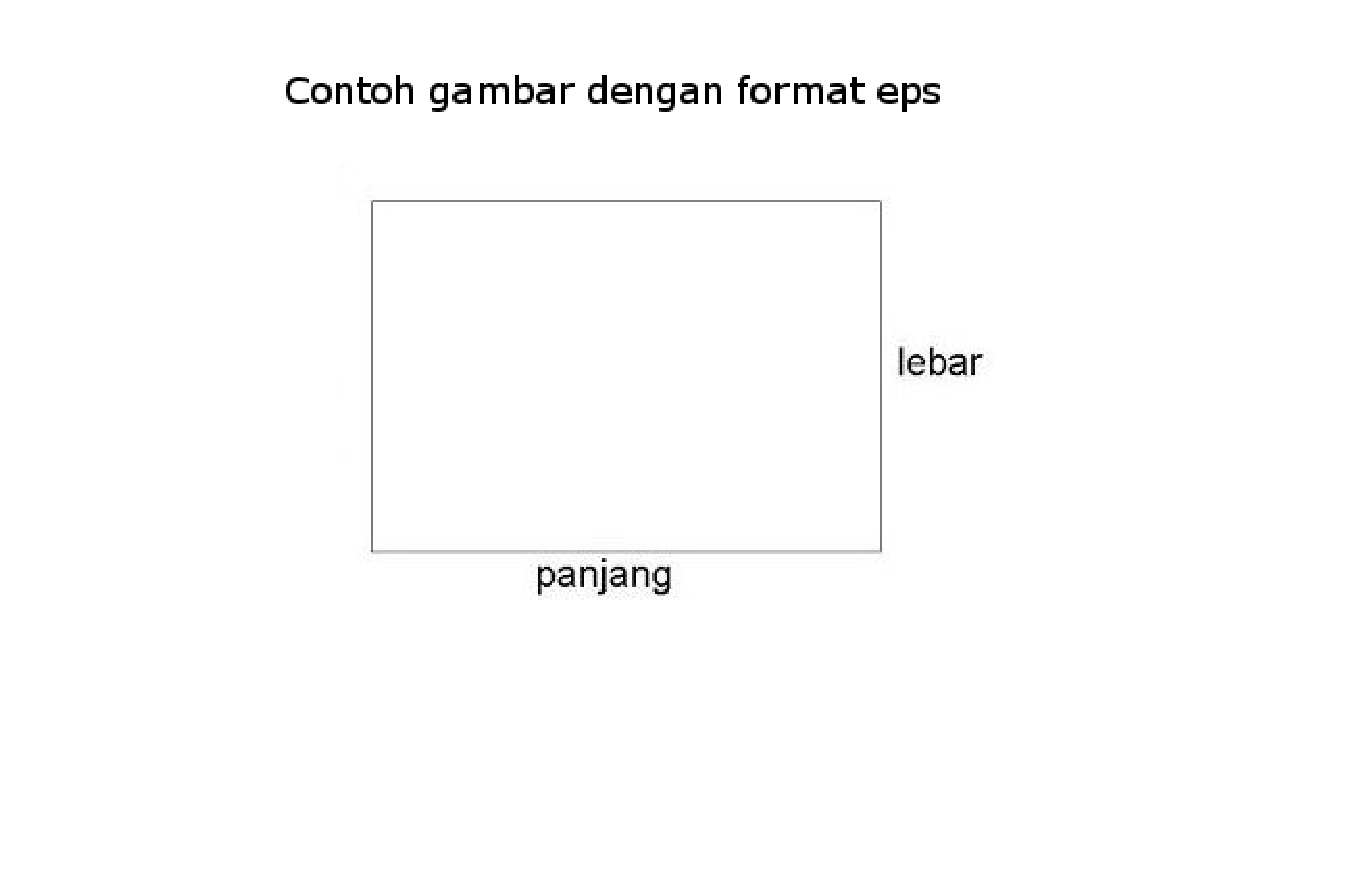
\includegraphics[width=0.8\columnwidth]{bab1/Gambar/gambar1-1.eps}
%\end{center}
%\vspace{-0.2cm}
%%\rule{\columnwidth}{0.1pt}
%\caption{Perbedaan Alur Desain FPGA dan Desain ASIC}\label{gambar1}
%\end{figure}
%%%%%%%%%%%%%%%%%%%%%%%%%%% GAMBAR %%%%%%%%%%%%%%%%%%%%%%%%%%%%%%

 %Bab 1
	\chapter{TELAAH PUSTAKA}
\label{cha:2-TelaahPustaka}

\vspace{1cm}
\section{\textit{Computer Vision}}
\hspace{1,2cm}\textit{Computer Vision} atau visi komputer adalah bidang kecerdasan buatan (AI) yang memungkinkan komputer dan sistem memperoleh informasi bermakna dari gambar digital, video, dan input visual lainnya, dan mengambil tindakan atau membuat rekomendasi berdasarkan informasi tersebut. Jika kecerdasan buatan memungkinkan komputer untuk berpikir, visi komputer memungkinkan untuk melihat, mengamati, dan memahami (IBM, 2020).

\textit{Computer vision} bekerja hamper sama dengan visi manusia, kecuali manusia memiliki permulaan. Penglihatan manusia memiliki keunggulan konteks seumur hidup untuk melatih cara membedakan objek, seberapa jauh jaraknya, apakah bergerak, dan apakah ada yang salah dalam sebuah gambar. \textit{Computer vision} melatih mesin untuk melakukan fungsi-fungsi melatih mesin untuk melakukan fungsi-fungsi ini, tetapi ia harus melakukannya dalam waktu yang jauh lebih singkat dengan kamera, data, dan algoritma daripada retina, saraf, optic, dan korteks visual karena sistem yang dilatih untuk memeriksa produk atau mengamati asset produksi dapat menganalisis ribuan produk atau proses dalam satu menit, memperhatikan cacat atau masalah yang tidak terlihat, sistem tersebut dapat dengan cepat melampaui kemampuan manusia. 

Memahami dan menentukan tugas visi komputer tertentu dapat memfokuskan dan memvalidasi proyek dan aplikasi, serta mempermudah untuk memulai. Hal dasar untuk \textit{computer vision} adalah \textit{object detection}, beberapa tugas visi komputer lainnya, seperti \textit{image classification, object detection, object tracking}, dan \textit{content-based image retrieval} (U. Arshad, 2021).

\vspace{1cm}
\section{Pengertian Citra}
Citra didefinisikan sebagai fungsi dari dua variabel misalnya \textit{a(x,y)} dimana a sendiri sebagai amplitudo (misalnya kecerahan) citra pada koordinat (x,y) (I. T. Young et al, 1995). Citra digital a[m,n] merupakan citra dalam ruang diskrit 2D yang berasal dari citra analog a(x,y) di ruang kontinyu 2D melalui proses sampling yaitu yang biasa disebut sebagai digitalisasi. Sedangkan, menurut Maria citra digital adalah citra f(x,y) yang telah didiskritkan oleh pada koordinat spasial dan kecerahan. Citra digital direpresentasikan oleh \textit{array} dua dimensi atau sekumpulan \textit{array} dua dimensi dimana setiap \textit{array} merepresentasikan satu kanal warna. Nilai kecerahan yang didigitalkan dinamakan nilai tingkat keabuan (A. McAndrew, 2004).

Setiap elemen \textit{array} tersebut dinamakan piksel yang diambil dari istilah \textit{picture element}. Dimensi citra biasanya ditulis dengan format panjang x tinggi (misalnya 640 x 480 piksel). Namun, perlu diperhatikan dengan seksama bahwa secara matematis, definisi citra terlihat seperti di bawah ini, dimana x menunjukkan baris dan y menunjukkan kolom:

\[
f(x,y)=
\begin{bmatrix}
	f\left(0,0\right)  & f\left(0,1\right) & ... & f\left(0,N-1\right) \\ 
	f\left(1,0\right)  & f\left(1,1\right) & ... & f\left(1,N-1\right) \\
	... & ... & ... & .. \\
	f\left(M-1,0\right) & f\left(M-1,1\right) & ... & \ f\left(M-1,N-1\right)
\end{bmatrix}
\]

Seperti pada layar monitor, koordinat citra dimulai dari pojok kiri atas. Secara matematis dimulai dari (0,0) dan berakhir di (M-1, N-1), dimana M menunjukkan tinggi, dan N menunjukkan panjang.

\section{Pengolahan Citra}
\hspace{1,2cm}Pengolahan citra adalah pemrosesan citra, khususnya menggunakan komputer menjadi citra yang kualitasnya lebih baik. Pengolahan citr adikembangkan bertujuan untuk (M. Petrou, 1999):
\begin{enumerate}
	\item Untuk memperbaiki tampilan citra (\textit{image enhancement}).
	\item Untuk mengurangi ukuran file citra dengan tetap mempertahankan kualitas citra (\textit{image compression}).
	\item Untuk memulihkan citra ke kondisi semula (\textit{image restoration}). 
	\item Untuk menyoroti ciri tertentu dari citra agar lebih mudah untuk di analisis. 
\end{enumerate}

Pengolahan citra adalah cabang ilmu informatika untuk memperbaiki kualitas citra agar kualitasnya lebih baik atau lebih mudah diinterpretasi oleh manusia maupun komputer. Input dari program pengolahan citra adalah citra dan outputnya pun citra pula.

Pengolahan citra digital digunakan dalam berbagai bidang untuk mempermudah manusia dalam melakukan analisis dan pekerjaan. Bentuk aplikasi pengolahan citra digital yang digunakan bidang militer, industry, medis, transportasi, hukum dan keamanan, pemetaan, robotika, fotografi, film, pencarian gambar berdasarkan kandungan citra, dan pemahaman kandungan citra. Salah satu pemanfaatan teknologi pengolahan citra digital yaitu bisa memahami maksud dari sebuah citra. Apabila aplikasi diberikan input berupa gambar yang mampu mendefinisikan bahwa dalam gambar tersebut terdapat gambar yang mendapati objek, seperti kendaraan, jalan, buah, dan lainnya.

\section{\textit{Artificial Intelligence} (AI)}
\hspace{1,2cm}\textit{Artificial inlelligence} atau kecerdasan buatan adalah studi tentang teori dan pengembangan sistem komputer agar mampu melakukan tugas-tugas yang dahulu hanya dapat dilakukan oleh manusia. Seperti membadakan berbagai gambar, menjawab pertanyaan, mengenali dan menerjemahkan bahasa, dan sebagainya (R. Primartha, 2018). 

Komputer atau mesin cukup bagus untuk melakukan hal-hal berikut: menyelesaikan perhitungan aritmatika dengan cepat, mengerjakan secara akurat apa-apa yang sudah deprogram oleh komputer. Namun, komputer atau mesin memiliki kelemahan, seperti sulit berinteraksi dengan \textit{noisy data} (data yang blur/bias), sulit memahami lingkungan, kurang toleran yerhadap kesalahan (\textit{fault tolerance}), sulit beradaptasi dengan situasi dan kondisi tertentu. Untuk mengatasi hal tersebut ada lima hal yang perlu dimiliki oleh mesin, yaitu:

\begin{enumerate}
	\item Persepsi
	
	Terkait dengen permasalahan pengindraan. Mesin harus memiliki indra untuk dapat mengenali dunia sekitarnya.
	
	\item Pemrosesan bahasa alami (NLP)
	
	Kemampuan untuk mengidentifikasi kalimat dan memahami perbedaan aksesn dan maknanya.
	
	\item Menyampaikan pengetahuan
	
	Menyampaikan berbagai informasi di dunia luar berdasarkan pemikirannya sendiri.
	
	\item Pengambilan keputusan
	
	Mampu memecahkan berbagai permasalahan secara logis.
	
	\item Perencanaan dan pemetaan
	
	Memetakan dunia tiga dimensi dan merencanakan rute paling efektif.
	Salah satu bagian penting dari AI adalah machine learning atau pembelajaran 
\end{enumerate}

Salah satu bagian penting dari AI adalah \textit{machine learning} atau pembelajaran mesin, yaitu dicirikan sebagai studi tentang algoritma dan model statistik yang digunakan sistem komputer untuk belajar dari data sampel dan pengalaman sebelumnya tanpa diprogram secara eksplisit untuk mencapai tugas tertentu. Dengan kemampuan untuk mengidentifikasi pola yang tidak jelas dalam data, kita dapat menggunakan pembelajaran mesin untuk memecahkan banyak masalah, termasuk menilai hubungan dua variabel, membuat prediksi berdasarkan karakteristik dasar, mengidentifikasi objek dengan pola yang sebanding, dan menggabungkan subjek dengan kriteria tertentu. Baik \textit{Artificial Intelligence}, \textit{Machine Learning}, dan \textit{Deep Learning} merupakan tiga istilah yang popular, namun banyak yang salah mengira bahwa ketiganya menggambarkan hal yang sama, padahal tiga hal yang berbeda. Bagaimana hubungan tiga istilah ini, seperti pada Gambar \ref{img:Hubungan-Artificial-Intelligence}

%%%%%%%%%%%%%%%%%%%%%%%%%% GAMBAR %%%%%%%%%%%%%%%%%%%%%%%%%%%%%%
\begin{figure}[H]
	\vspace{-0.1cm}
	%\rule{\columnwidth}{0.1pt}
	\begin{center}
		\includegraphics[width=1\columnwidth]{bab2/Gambar/Picture1.jpg}
	\end{center}
	\vspace{-0.2cm}
	%\rule{\columnwidth}{0.1pt}
	\caption{(a) Hubungan Artificial Intelligence, Machine Learning, dan Deep Learning. (b) Jenis Machine Learning\\(Sumber: C. Thongprayoon et al, 2020)}\label{img:Hubungan-Artificial-Intelligence}
\end{figure}
%%%%%%%%%%%%%%%%%%%%%%%%%% GAMBAR %%%%%%%%%%%%%%%%%%%%%%%%%%%%%%

Disamping hal tersebut, \textit{artificial intelligence} (AI) memungkinkan untuk berfikir, dan salah satu bagian dari \textit{artificial intelligence} untuk dapat melihat, mengamati, dan memahami adalah komputer visi atau \textit{computer vision}. \textit{Computer vision} memungkinkan untuk komputer dan sistem memberikan informasi berarti dari gambar digital, dan visual input. 

\section{\textit{Object Detection}}
\hspace{1,2cm}\textit{Object detection} atau deteksi objek dianggap sebagai salah satu bidang penting dalam pembelajaran mendalam dan visi komputer. Deteksi objek telah ditentukan oleh banyak aplikasi dalam visi komputer, seperti pelacakan objek, pengambilan, dan pengawasan video. Deteksi objek adalah teknologi \textit{deep learning} dimana benda, manusia, bengunan, mobil, dapat dideteksi sebagai objek dalam gambar dan video (U. Arshad, 2021).

Deteksi objek untuk mengenali objek dengan kotak pembatas pada gambar, dimana dalam klasifikasi gambar, cukup mengkategorikan (mengklasifikasikan) objek pada gambar atau tidak dalam hal kemungkinan (\textit{probability}), seperti contoh pada Gambar \ref{img:Classification-Object-Detection}

%%%%%%%%%%%%%%%%%%%%%%%%%% GAMBAR %%%%%%%%%%%%%%%%%%%%%%%%%%%%%%
\begin{figure}[H]
	\vspace{-0.1cm}
	%\rule{\columnwidth}{0.1pt}
	\begin{center}
		\includegraphics[width=1\columnwidth]{bab2/Gambar/Picture2.png}
	\end{center}
	\vspace{-0.2cm}
	%\rule{\columnwidth}{0.1pt}
	\caption{Classification, Object Detection dan Segmentation Representation\\(Sumber: A. Patel, 2020)}\label{img:Classification-Object-Detection}
\end{figure}
%%%%%%%%%%%%%%%%%%%%%%%%%% GAMBAR %%%%%%%%%%%%%%%%%%%%%%%%%%%%%%

Pada Gambar \ref{img:Segementation-Classification}, terlihat bahwa kucing (cat) dengan kotak pembatas dan tanpa kotak pembatas dapat membedakan mendasar antara klasifikasi citra dan deteksi objek.

%%%%%%%%%%%%%%%%%%%%%%%%%% GAMBAR %%%%%%%%%%%%%%%%%%%%%%%%%%%%%%
\begin{figure}[H]
	\vspace{-0.1cm}
	%\rule{\columnwidth}{0.1pt}
	\begin{center}
		\includegraphics[width=1\columnwidth]{bab2/Gambar/Picture3.png}
	\end{center}
	\vspace{-0.2cm}
	%\rule{\columnwidth}{0.1pt}
	\caption{Segmentation, Classification+Localization, Object Detection\\(Sumber: A. Patel, 2020)}\label{img:Segementation-Classification}
\end{figure}
%%%%%%%%%%%%%%%%%%%%%%%%%% GAMBAR %%%%%%%%%%%%%%%%%%%%%%%%%%%%%%

Dalam mempelajari deteksi objek, maka diperlukan mengetahui klasifikasi citra (\textit{image classification}). Ketika gambar adalah input ke CNN, masalah mengklasifikasikan kelas yang sesuai dengan gambar dikenal sebagai klasifikasi gambar, dan seperti yang ditunjukkan pada Gambar \ref{img:Image-Classification}, nilai probabilitas untuk semua kelas yang ditargetkan adalah keluaran.

%%%%%%%%%%%%%%%%%%%%%%%%%% GAMBAR %%%%%%%%%%%%%%%%%%%%%%%%%%%%%%
\begin{figure}[H]
	\vspace{-0.1cm}
	%\rule{\columnwidth}{0.1pt}
	\begin{center}
		\includegraphics[width=1\columnwidth]{bab2/Gambar/Picture4.png}
	\end{center}
	\vspace{-0.2cm}
	%\rule{\columnwidth}{0.1pt}
	\caption{Image Classification\\(Sumber: A. Patel, 2020)}\label{img:Image-Classification}
\end{figure}
%%%%%%%%%%%%%%%%%%%%%%%%%% GAMBAR %%%%%%%%%%%%%%%%%%%%%%%%%%%%%%

Dapat juga dianggap bahwa deteksi objek sebagai masalah dimana tugas klasifikasi gambar memiliki tugas regresi yang memprediksi posisi objek menggunakan \textit{bounding box} (kotak pembatas) pada Gambar \ref{img:Object-Bounding-Box}. 

%%%%%%%%%%%%%%%%%%%%%%%%%% GAMBAR %%%%%%%%%%%%%%%%%%%%%%%%%%%%%%
\begin{figure}[H]
	\vspace{-0.1cm}
	%\rule{\columnwidth}{0.1pt}
	\begin{center}
		\includegraphics[width=1\columnwidth]{bab2/Gambar/Picture5.png}
	\end{center}
	\vspace{-0.2cm}
	%\rule{\columnwidth}{0.1pt}
	\caption{Object Detection dengan Bounding Box\\(Sumber: A. Patel, 2020)}\label{img:Object-Bounding-Box}
\end{figure}
%%%%%%%%%%%%%%%%%%%%%%%%%% GAMBAR %%%%%%%%%%%%%%%%%%%%%%%%%%%%%%

Masalah deteksi objek mengasumsikan bahwa beberapa kelas objek mungkin ada dalam gambar pada waktu yang sama. Dapat memvisualisasikan seperti dua jenis masalah, 1) klasifikasi multi label (beberapa kelas dalam satu gambar), 2) Bounding Box (masalah regresi) dimana harus memprediksi nilai koordinat kotak pembatas (\textit{bounding box}) dalam bentuk x, y, w, h.

Dalam deteksi objek, terdapat \textit{object localization} atau lokalisasi objek yang merupakan untuk memprediksi objek dalam sebuah citra serta batas-batasnya. Perbedaan antara lokalisasi objek dan deteksi objek tidak kentara. Sederhananya, lokalisasi objek bertujuan untuk menemukan objek utama (atau yang paling terlihat) dalam sebuah gambar, sedangkan deteksi objek mencoba untuk mengetahui semua objek dan batasannya.

Suatu klasifikasi citra atau model pengenalan citra hanya mendeteksi probabilitas suatu objek dalam suatu citra. Berbeda dengan ini, lokalisasi objek mengacu pada mengidentifikasi lokasi suatu objek dalam gambar. Algoritma lokalisasi objek akan menampilkan koordinat lokasi objek sehubungan dengan gambar. Dalam visi komputer, cara paling popular untuk melokalkan objek dalam gambar adalah dengan merepresentasikan lokasinya dengan bantuan kotak pembatas (\textit{bounding box}).

Bounding box dapat diinisialisasi menggunakan parameter berikut: 
\begin{itemize}
	\item bx, by: koordinat pusat kotak pembatas (center of bounding box)
	\item bw: lebar kotak pembatas dengan lebar gambar (width)
	\item bh: tinggi kotak pembatas dengan tinggi gambar (height)
\end{itemize}

%%%%%%%%%%%%%%%%%%%%%%%%%% GAMBAR %%%%%%%%%%%%%%%%%%%%%%%%%%%%%%
\begin{figure}[H]
	\vspace{-0.1cm}
	%\rule{\columnwidth}{0.1pt}
	\begin{center}
		\includegraphics[width=1\columnwidth]{bab2/Gambar/Picture6.png}
	\end{center}
	\vspace{-0.2cm}
	%\rule{\columnwidth}{0.1pt}
	\caption{Intersection Over Union (IoU)\\(Sumber: A. Patel, 2020)}\label{img:Intersection-Over-Union}
\end{figure}
%%%%%%%%%%%%%%%%%%%%%%%%%% GAMBAR %%%%%%%%%%%%%%%%%%%%%%%%%%%%%%

Dengan memprediksi ini, dapat menghitung Mean-IoU dan memprediksi kotak pembatas (\textit{bounding box}) yang melokalkan objek di gambar.
\begin{itemize}
	\item IoU adalah Intersection-Over-Union (IoU) disebut sebagai Indeks Jaccard (\textit{Jaccard Index}) dianggap sebagai salah satu metrik kinerja yang paling banyak digunakan dalam deteksi objek. 

%%%%%%%%%%%%%%%%%%%%%%%%%% GAMBAR %%%%%%%%%%%%%%%%%%%%%%%%%%%%%%
\begin{figure}[H]
	\vspace{-0.1cm}
	%\rule{\columnwidth}{0.1pt}
	\begin{center}
		\includegraphics[width=0.4\columnwidth]{bab2/Gambar/Picture7.png}
	\end{center}
	\vspace{-0.2cm}
	%\rule{\columnwidth}{0.1pt}
	\caption{Persamaan IoU\\(Sumber: A. Patel, 2020)}\label{img:Persamaan-IOU}
\end{figure}
%%%%%%%%%%%%%%%%%%%%%%%%%% GAMBAR %%%%%%%%%%%%%%%%%%%%%%%%%%%%%%

	\item IoU adalah area tumpang tindih (\textit{overlap}) antara segmentasi yang diprediksi (\textit{prediction}) dan kebenaran dasar (\textit{ground truth}), seperti yang ditampilkan pada Gambar \ref{img:Persamaan-IOU}. Metrik ini bervariasi dari 0-1 (0-100\%) dengan 0 menyiratkan tidak ada tumpeng tindih (sampah) dan 1 menandakan segmentasi yang tumpang tindih sempurna (\textit{fat dub}).
	
	\item Mean IoU adalah segmentasi biner (dua kelas) atau multi-kelas, mean Io Udari gambar dihitung dengan mengambil IoU dari setiap kelas dan merata-ratakannya. 

\end{itemize}

\section{Machine Learning}
\hspace{1,2cm}Istilah \textit{machine learning} mula-mula diperkenalkan oleh Arthur Samuel pada tahun 1959 melalui jurnalnya yang berjudul "Some Studies in Machine Learning Using the Game of Checkers". (IBM Journal of Research and Development). Samuel mencoba mengajari program komputer untuk bermain catur. Tujuannya adalah membuat agar komputer dapat bermain catur lebih baik dari dirinya. Pada tahun 1962 program buatannya dapat mengalahkan juara catur dari negara bagian Connecticut (R. Primartha, 2018).

\textit{Machine learning} membutuhkan sebuah model yang didefinisikan berdasar parameter-parameter tertentu. Proses learning adalah eksekusi program komputer untuk mengoptimasi parameter-parameter dari model tersebut, dengan memanfaatkan data training atau \textit{past experience}.

Jadi, secara sederhana dapat dijelaskan bahwa \textit{machine learning} adalah pemrograman komputer untuk mencapai kriteria/performa tertentu dengan menggunakan sekumpulan data training atau pengalaman di masa lalu (\textit{past experience}). \textit{Machine learning} mempelajari teori agar komputer mampu "belajar" dari data. 

Secara umum algoritma \textit{machine learning} dapat dikelompokkan menjadi lima bagian, yaitu \textit{supervised learning}, \textit{unsupervised learning}, \textit{semi-supervised learning}, \textit{reinforcement learning}, dan \textit{deep learning}.

\subsection{Supervised Learning} 
\hspace{1,2cm}Sebagian besar praktik machine learning mengandalkan algoritma \textit{supervised learning}. Algoritmanya dinamakan seperti ini karena training dataset (sekumpulan data untuk training) akan memandu dan mengajari komputer agar menghasilkan outcome sesuai harapan. Pada \textit{supervised learning} menggunakan sebuah algoritma untuk mempelajari mapping function antara input dengan output. Berbagai kemungkinan output sudah diketahui dan data-data yang digunakan untuk latihan (training) sudah diberi label dengan jawaban yang benar. \textit{Supervised learning} dapat bermanfaat untuk memprediksi sesuatu dengan bantuan training dataset. Berikut skema \textit{supervised learning} pada Gambar \ref{img:Skema-Supervised-Learning} (R. Primartha, 2018).

%%%%%%%%%%%%%%%%%%%%%%%%%% GAMBAR %%%%%%%%%%%%%%%%%%%%%%%%%%%%%%
\begin{figure}[H]
	\vspace{-0.1cm}
	%\rule{\columnwidth}{0.1pt}
	\begin{center}
		\includegraphics[width=1\columnwidth]{bab2/Gambar/Picture8.png}
	\end{center}
	\vspace{-0.2cm}
	%\rule{\columnwidth}{0.1pt}
	\caption{Skema Supervised Learning\\(Sumber: M. Kozan, 2021)}\label{img:Skema-Supervised-Learning}
\end{figure}
%%%%%%%%%%%%%%%%%%%%%%%%%% GAMBAR %%%%%%%%%%%%%%%%%%%%%%%%%%%%%%

\textit{Supervise learning} menggunakan training data yang sudah diberi label untuk mempelajari \textit{mapping function}, dari input variables (x) ke ouput variables (y).
\[y=f\ (x)\]

Sebagai contoh, sebuah algoritma klasifikasi akan dapat mengidentifikasi berbagai bentuk bangun setelah melalui proses belajar dari sekumpulan bangun datar yang sudah ditandai atau diberi label dengan ciri tertentu seperti pada gambar 2.12.

Permasalahan-permasalahan yang terkait dengan \textit{supervised learning} dapat dikategorikan menjadi dua jenis:
\begin{enumerate}
	\item \textit{Classification}
	
	Klasifikasi bertujuan untuk memprediksi outcome dari input (sample yang diberikan), dimana output variabel berbentuk kategori-kategori. Contoh: pria/wanita, sakit/sehat, tinggi/rendah, dan sebagainya.
	
	\item \textit{Regression}
	
	Regression bertujuan untuk memprediksi outcome dari input (sample yang diberikan), dimana output, variabel berbentuk nilai aktual (\textit{real values}). Contoh: prediksi harga rumah, tinggi badan seseorang, curah hujan, dan sebagainya. 
	
\end{enumerate}

Ada beberapa algoritma yang sudah dikembangkan dan terkait dengan \textit{supervised learning}, diantaranya:
\begin{enumerate}
	\item Decision tree,
	\item Naïve Bayes Classifier,
	\item Artificial Neural Network,
	\item Support Vector Machine,
	\item Linear Regression,
	\item Logistic Regression,
	\item CART,
	\item KNN (-KNearest Neighbor), dsb.
\end{enumerate}

\subsection{Unsupervised Learning}
\hspace{1,2cm}Berbeda dengan supervised learning, pada \textit{unsupervised learning} persoalan diproses hanya mengandalkan data yang belum dilatih sebelumnya. \textit{Unsepervised learning} menggunakan \textit{unlabeled training dataset} untuk memodelkan struktur dari data, sehingga unsupervised learning bersifat lebih subjektif dibandingkan \textit{supervised learning}. Berikut skema \textit{unsupervised learning} pada Gambar \ref{img:Skema-Unsupervised-Learning} (R. Primartha, 2018).

%%%%%%%%%%%%%%%%%%%%%%%%%% GAMBAR %%%%%%%%%%%%%%%%%%%%%%%%%%%%%%
\begin{figure}[H]
	\vspace{-0.1cm}
	%\rule{\columnwidth}{0.1pt}
	\begin{center}
		\includegraphics[width=1\columnwidth]{bab2/Gambar/Picture9.png}
	\end{center}
	\vspace{-0.2cm}
	%\rule{\columnwidth}{0.1pt}
	\caption{Skema Unsupervised Learning\\(Sumber: M. Kozan, 2021)}\label{img:Skema-Unsupervised-Learning}
\end{figure}
%%%%%%%%%%%%%%%%%%%%%%%%%% GAMBAR %%%%%%%%%%%%%%%%%%%%%%%%%%%%%%

\textit{Unsupervised learning} bermanfaat untuk kasus-kasus dimana kita ingin menemukan relasi implisit (implicit relationships) dari \textit{unlabeled dataset} yang disediakan. Jadi, pada \textit{unsupervised learning} kita tidak memprediksi masa depan, sebab input variable (X) tidak memiliki relasi dengan output variabel (Y). 
\[ f(x) \]

Untuk memudahkan memahaminya, dapat diasumsikan saat ini belum pernah membeli majalah sama sekali. Suatu ketika membeli beberapa buah majalah dan ingin membaginya menjadi beberapa kategori, dengan tujuan agar nantinya mudah dicari. Maka, dapat dimulai dengan mengidentifikasi majalah-majalah berdasarkan kemiripan. Misalnya, berdasarkan isi, penerbit, dan lain-lain yang bisa ditentukan sesuai kebutuhan.

Permasalahan seputar \textit{unsupervised learning} dapat dikelompokkan menjadi tiga kategori, yaitu:

\begin{enumerate}
	\item Association
	
	Association bertujuan untuk menemukan peluang (probabilitas) berdasarkan keterkaitan (co-occurrence) dari item-item dalam sebuah kumpulan. Sebuah contoh, jika customer membeli teh celup, maka kemungkinan besar (sekitar 80%) customer juga membeli gula pasir. Association banyak digunakan dalam market-basket analisis. 
	\item Clustering
	
	Clustering bertujuan untuk mengelompokkan sample dalam cluster yang sama berdasarkan kemiripan (similiarity).
	
	\item Dimensionality Reduction
	
	Dimensionality Reduction berarti mengurangi sejumlah variabel dari dataset namun tetap memastikan informasi yang penting masih tersedia. Dimensionality Reduction dapat diwujudkan menggunakan metode:
	\begin{enumerate}[label=(\alph*)]
		\item Feature Extraction
		
		Melakukan transformasi data dari dimensi tinggi (a high-dimensional space) ke dimensi yang lebih rendah (a low-dimensional space).
		
		\item Feature Selection
		
		Memilih Sebagian saja (subset) dari variabel asal (original variabel). 
	\end{enumerate}
\end{enumerate}

Beberapa algoritma yang dikelompokkan dalam \textit{unsupervised learning}, antara lain: 
\begin{enumerate}
	\item K-Means
	\item Hierarchical Clustering
	\item DBSCAN
	\item Fuzzy C-Means
	\item Self-Orginizing Map, dan sebagainya.	
	
\end{enumerate}

\subsection{Semi-supervised learning}
\hspace{1,2cm}Metode ini berada diantara yang \textit{supervised} dan \textit{unsupervised learning} di mana memiliki sejumlah besar masukan data, beberapa di antaranya diberi label dan sisanya tidak. Banyak masalah pembelajaran kehidupan nyata termasuk dalam bidang pembelajaran mesin ini. Alasannya adalah \textit{semi-supervised} membutuhkan lebih sedikit intervensi manusia karena menggunakan data berlabel dalam jumlah yang sangat kecil dan data yang tidak berlabel dalam jumlah besar. Memanfaatkan kumpulan data yang kurang berlabel lebih menarik karena kumpulan data tersebut sangat sulit untuk dikumpulkan serta mahal dan mungkin memerlukan akses ke pakar domain. Dataset yang tidak berlabel di sisi lain lebih murah dan lebih mudah diakses (X. Zhu, 2018).

Kedua teknik pembelajaran \textit{supervised} dan \textit{unsupervised learning} bisa digunakan untuk melatih algoritma pembelajaran dalam pembelajaran \textit{semi-supervised}. Teknik \textit{unsupervised learning} dapat digunakan untuk mengungkap struktur dan pola tersembunyi dalam kumpulan data input. Sedangkan teknik supervised learning dapat digunakan untuk membuat prediksi tebakan pada data yang tidak berlabel, memasukkan data kembali ke algoritma pembelajaran sebagai data pelatihan, dan menggunakan pengetahuan yang diperoleh untuk membuat prediksi pada kumpulan data baru. Dengan demikian, dapat mengatakan bahwa data yang tidak berlabel digunakan untuk memodifikasi atau memprioritaskan kembali prediksi atau hipotesis yang diperoleh dari data yang berlabel. Gambar \ref{img:Skema-Semi-Supervised-Learning} mengilustrasikan berbagai tahapan metode \textit{semi-supervised learning}.

%%%%%%%%%%%%%%%%%%%%%%%%%% GAMBAR %%%%%%%%%%%%%%%%%%%%%%%%%%%%%%
\begin{figure}[H]
	\vspace{-0.1cm}
	%\rule{\columnwidth}{0.1pt}
	\begin{center}
		\includegraphics[width=1\columnwidth]{bab2/Gambar/Picture10.png}
	\end{center}
	\vspace{-0.2cm}
	%\rule{\columnwidth}{0.1pt}
	\captionsetup{justification=centering}
	\caption{Skema Semi-Supervised Learning\\(Sumber: A. B. Nassif et al, 2019)}\label{img:Skema-Semi-Supervised-Learning}
\end{figure}
%%%%%%%%%%%%%%%%%%%%%%%%%% GAMBAR %%%%%%%%%%%%%%%%%%%%%%%%%%%%%%

Untuk memanfaatkan data pelatihan yang tidak berlabel, semua algoritma \textit{semi-supervised learning} melakukan setidaknya satu dari asumsi berikut asumsi kehalusan, asumsi cluster, dan asumsi manifold.

\subsection{Reinforcement Learning}
\hspace{1,2cm}\textit{Reinforcement learning} merupakan metode pembelajaran yang dipengaruhi oleh feedback dari lingkungan dengan Teknik pembelajaran yang iterative (berulang-ulang) dan adaptive (menyesuaikan). \textit{Reinforcement learning} dipercaya mendekati cara manusia belajar (R. Primartha, 2018). 

\textit{Reinforcement learning} (RL) diinspirasi oleh kebiasaan makhluk hidup dalam belajar dan bertindak, khususnya manusia. Pada RL tidak ada dataset. Data-data diperoleh berdasarkan pengalaman. Algoritma \textit{reinforcement learning} mengijinkan agent untuk memutuskan aksi selanjutnya berdasarkan kondisi saat ini (\textit{current state}). \textit{Reinforcement learning} kadang disebut juga \textit{credit assessment learning}, sebab learning difokuskan untuk memaksimalkan perolehan \textit{rewards}. \textit{Reinforcement learning} tergantung pada proses coba-coba untuk mengungkap rangkaian tindakan yang memaksimalkan metrik imbalan kumulatif, yang digunakan untuk membuat algoritma memahami apakah itu mengarah ke arah yang benar atau tidak. Berikut skema \textit{reinforcement learning} pada Gambar \ref{img:Skema-Reinforcement-Learning}. 

%%%%%%%%%%%%%%%%%%%%%%%%%% GAMBAR %%%%%%%%%%%%%%%%%%%%%%%%%%%%%%
\begin{figure}[H]
	\vspace{-0.1cm}
	%\rule{\columnwidth}{0.1pt}
	\begin{center}
		\includegraphics[width=1\columnwidth]{bab2/Gambar/Picture11.png}
	\end{center}
	\vspace{-0.2cm}
	%\rule{\columnwidth}{0.1pt}
	\captionsetup{justification=centering}
	\caption{Skema Reinforcement Learning\\(Sumber: R. Sutton, 1998)}\label{img:Skema-Reinforcement-Learning}
\end{figure}
%%%%%%%%%%%%%%%%%%%%%%%%%% GAMBAR %%%%%%%%%%%%%%%%%%%%%%%%%%%%%%

Menurut R. Sutton, proses \textit{reinforcement learning} dapat dipresentasikan dalam matematika sebagai \textit{Markov Decision Process} (MDP), memperkenalkan 4 set {S, A, P, R}, dengan:\\
S - Kumpulan status tempat agen dapat berada, pada saat tertentu;\\
A - Serangkaian kemungkinan Tindakan yang dapat dilakukan agen dalam waktu tertentu;\\
P - Himpunan probabilitas, bahwa sebuah agen, yang berada dalam keadaan s, bertransisi ke keadaan s' dengan melakukan Tindakan A dalam waktu t+1;

Representasi \textit{reinforcement learning} mirip dengan supervised learning. Yang membedakan adalah pada reinforcement learning tidak hanya x, namun x dan z.
\[ y=\ f\ \left(x\right)\ given\ z \]

Tidak seperti \textit{supervised} dan \textit{unsupervised learning} dimana algoritma sudah memiliki tujuan (goal). Algoritma \textit{reinforcement learning} tidak memiliki tujuan eksplisit, sebagai gantinya algoritma dipaksa untuk belajar menemukan nilai optimal melalui kegiatan trial dan error.

\textit{Reinforcement learning} banyak diimplementasikan pada \textit{game theory, control theory, operation research, information theory, simulation-based optimaztion, multi-agent systems, swarm intelligence, statistics}, dan \textit{genetic algorithm}.

Contoh penerapan \textit{reinforcement learning} yaitu pada bidang robotic. Sebuah robot dapat belajar untuk menghindari tabrakan dengan cara menerima feedback negative manakala robot tersebut menabrak halangan tertentu. Robot akan dibiarkan berjalan tanpa dipandu. Robot akan belajar dari pengalaman sebelumnya untuk menemukan rute paling optimal. 

Beberapa algoritma yang dikelompokkan dalam \textit{reinforcement learning} antara lain:
\begin{enumerate}
	\item Genetic Algorithm (GA)
	\item Dynamic Programming (DP)
	\item Generalized Policy Iteration (GPI)
	\item Monte Carlo Methods
\end{enumerate}

\subsection{Deep Learning}
\hspace{1,2cm}\textit{Deep learning} merupakan metode pembelajaran yang memanfaatkan \textit{artificial neural networks} yang berlapis-lapis (multi layer). \textit{Artificial neural networks} ini dibuat mirip dengan otak manusia, di mana neuron-neuron terkoneksi satu sama lain, sehingga membentuk sebuah jaringan neuron yang sangat rumit (R. Primartha, 2018).

\textit{Deep learning} atau \textit{deep structured leaning} atau hierarchical learning atau deep neural merupakan metode pembelajaran yang memanfaatkan multiple non-linear transformation. \textit{Deep learning} dapat dipandang sebagai gabungan machine learning dengan \textit{artificial intelligence} (AI). \textit{Deep learning} pada hakekatnya merupakan perluasan atau pengembangan dari \textit{neural network} atau jaringan saraf tiruan (JST).

Jika dikembalikan kepada tujuan \textit{machine learning} semula, yaitu komputer yang dapat belajar (dari data atau pengalaman), maka \textit{deep learning} adalah apa yang selama ini dicari. \textit{Deep learning} menirukan cara berpikir manusia. Pada \textit{deep learning}, komputer harus memproses data yang sangat banyak, berlapis-lapis, dan output dari layer sebelumnya akan menjadi input bagi layer sesudahnya.

Struktur umum dan dasar dari skema \textit{deep learning} ditunjukkan pada Gambar \ref{img:Skema-Umum-Deep-Learning}. Ini terdiri dari lapisan masukan, yang merupakan data masukan ke algoritma; lapisan tersembunyi, di mana algoritma membuat banyak perhitungan matematis, dan lapisan output, yang merupakan hasil dari perhitungan algoritma.

%%%%%%%%%%%%%%%%%%%%%%%%%% GAMBAR %%%%%%%%%%%%%%%%%%%%%%%%%%%%%%
\begin{figure}[H]
	\vspace{-0.1cm}
	%\rule{\columnwidth}{0.1pt}
	\begin{center}
		\includegraphics[width=1\columnwidth]{bab2/Gambar/Picture12.png}
	\end{center}
	\vspace{-0.2cm}
	%\rule{\columnwidth}{0.1pt}
	\captionsetup{justification=centering}
	\caption{Skema Umum \textit{Deep Learning}\\(Sumber: A. Feizollah et al, 2022)}\label{img:Skema-Umum-Deep-Learning}
\end{figure}
%%%%%%%%%%%%%%%%%%%%%%%%%% GAMBAR %%%%%%%%%%%%%%%%%%%%%%%%%%%%%%
Sejarah \textit{deep learning} dimulai pada tahun 2006, yaitu setelah Geoffrey Hinton mempublikasikan paper yang memperkenalkan salah satu varian \textit{neural networks} yang disebut \textit{deep belief nets}. Paper ini merupakan awal kemunculan istilah \textit{deep learning}, untuk membedakan arsitektur \textit{neural network} konvensional (\textit{single layer}) dengan arsitektur neural network multi/banyak layer. Dengan kata lain, deep learning adalah salah satu cabang machine learning yang menggunakan \textit{deep neural network} untuk menyelesaikan permasalahan pada domain \textit{machine learning}. 

Pada tahun 2009, Andrew memperkenalkan penggunaan GPU untuk \textit{deep learning} melalui paper yang berjudul \textit{large-scale deep unsupervised learning using graphics processors}. Dengan menggunakan GPU, algoritma \textit{deep learning} dapat dijalankan lebih cepat disbanding dengan tanpa GPU (hanya menggunakan CPU), Perkembangan \textit{deep learning} maju pesat berkat keberadaan \textit{hardware} yang memadai. Dan saat ini, \textit{deep learning} sudah banyak diaplikasikan di berbagai area, seperti pengenal wajah, \textit{self-driving car}, pengenal suara, dan sebagainya. 

\textit{Deep learning} merupakan jalan untuk mencapai apa yang sudah dicita-citakan sebelumnya oleh manusia, yaitu kecerdasan buatan bagi mesin. Bentuk diagram \textit{network model deep learning} seperti pada Gambar \ref{img:Skema-Deep-Learning-Hidden-Layer}. Perhatikan bahwa \textit{hidden layer} hanya digambarkan tiga lapis saja, padahal kenyataanya bisa berjumlah sangat banyak, dapat diasumsikan seperti Gambar \ref{img:Skema-Deep-Learning-Hidden-Layer}.

%%%%%%%%%%%%%%%%%%%%%%%%%% GAMBAR %%%%%%%%%%%%%%%%%%%%%%%%%%%%%%
\begin{figure}[H]
	\vspace{-0.1cm}
	%\rule{\columnwidth}{0.1pt}
	\begin{center}
		\includegraphics[width=1\columnwidth]{bab2/Gambar/Picture13.png}
	\end{center}
	\vspace{-0.2cm}
	%\rule{\columnwidth}{0.1pt}
	\captionsetup{justification=centering}
	\caption{Skema \textit{Deep Learning} dengan Penambahan beberapa \textit{hidden layer}\\(Sumber: H. Kaur et al, 2021)}\label{img:Skema-Deep-Learning-Hidden-Layer}
\end{figure}
%%%%%%%%%%%%%%%%%%%%%%%%%% GAMBAR %%%%%%%%%%%%%%%%%%%%%%%%%%%%%%

Pada Gambar \ref{img:Skema-Deep-Learning-Hidden-Layer} mengandung 3 layer, yaitu input, \textit{hidden} dan output layer. Penambahan \textit{layer} ini terjadi pada \textit{hidden layer}. \textit{Hidden layer} pada skema \textit{deep learning} yang disebut dengan \textit{Multi Layer Peceptron} (MLP) disebabkan jumlah neuron semakin banyak dan itu artinya semakin banyak juga perhitungan yang harus dikerjakan pada setiap \textit{layer}. MLP merupakan pengembangan dari \textit{Single Layer Perceptron} (SLP) yang merupakan model paling sederhana dari neural network dan sekaligus merupakan dasar bagi model-model tingkat lanjut yang digunakan pada \textit{deep learning}. MLP kemudian menjadi cikal bakal metode \textit{deep learning} atau \textit{deep neural network} (DNN).

\textit{Deep learning} sudah dikembangkan ke berbagai model atau arsitektur yang berbeda-beda. Berikut daftar beberapa model atau arsitektur untuk \textit{deep learning}. 
\begin{enumerate}
	\item \textit{Recurrent Neural Networks} (RNN)
	\item \textit{Long Short-Term Memory} (LSTM)
	\item \textit{Convolutional Neural Network} (CNN)
	\item \textit{Deep Believe Networks} (DBN)
	\item \textit{Deep Stacking Networks} (DSN)
\end{enumerate}

Contoh penerapan masing-masing arsitektur deep learning dapat dipelajari pada Tabel \ref{tbl:Penerapan-Arsitektur-Deep-Learning}
%%%%%%%%%%%%%%%%%%%%%%%TABEL SEDERHANA%%%%%%%%%%%%%%%%%%%%%%%%%
\begin{singlespace}
	\begin{table}[H]
		\centering
		\caption{Penerapan Arsitektur Deep Learning}
		\label{tbl:Penerapan-Arsitektur-Deep-Learning}
		\begin{adjustbox}{width=\columnwidth,center}
			\begin{tabular}{|c|c|l|}
				\hline
				No. & Arsitektur & \multicolumn{1}{c|}{Penerapan}                                                                                                                                           \\ \hline
				1   & RNN        & \textit{Speech recognition, handwriting recognition}                                                                                                                     \\ \hline
				2   & LSTM       & \textit{\begin{tabular}[c]{@{}l@{}}Natural language text compression, handwriting recognition,\\ speech recognition, gesture recognition, image captioning\end{tabular}} \\ \hline
				3   & CNN        & \textit{Image recognition, video analysis, natural language processing}                                                                                                  \\ \hline
				4   & DBN        & \textit{\begin{tabular}[c]{@{}l@{}}Image recognition, information retrieval, \\ natural language understanding, failure prediction\end{tabular}}                         \\ \hline
				5   & DSN        & \textit{Information retrieval, continuous speech recognition}                                                                                                            \\ \hline
			\end{tabular}
		\end{adjustbox}
	\end{table}
\end{singlespace}
%%%%%%%%%%%%%%%%%%%%%%%TABEL SEDERHANA%%%%%%%%%%%%%%%%%%%%%%%%%
Masing-masing arsitektur pada Tabel \ref{tbl:Penerapan-Arsitektur-Deep-Learning} memiliki perbedaan, berikut penjelasan dan diagram network beberapa arsitektur deep learning yang umum.

\subsubsection{Recurrent Neural Networks (RNN)}
\hspace{1,2cm}\textit{Recurrent Neural Network} (RNN) merupakan arsitektur \textit{deep learning} yang popular serta sangat menjanjinak untuk menyelesaikan berbagai persoalan yang terkait dengan \textit{Natural Language Processing} (NLP). Model RNN digunakan agar mesin dapat memahami bahasa manusia. Mulai dari cara berkomunikasi, mendengarkan, mengenali percakapan, hingga memahami tata bahasa dan aksen. RNN juga dapat diimplementasikan untuk mengenali gambar-gambar atau objek (R. Primartha, 2018).

Diagram network RNN seperti pada Gambar \ref{img:Diagram-RNN} berikut. 
%%%%%%%%%%%%%%%%%%%%%%%%%% GAMBAR %%%%%%%%%%%%%%%%%%%%%%%%%%%%%%
\begin{figure}[H]
	\vspace{-0.1cm}
	%\rule{\columnwidth}{0.1pt}
	\begin{center}
		\includegraphics[width=0.8\columnwidth]{bab2/Gambar/Picture14.png}
	\end{center}
	\vspace{-0.2cm}
	%\rule{\columnwidth}{0.1pt}
	\captionsetup{justification=centering}
	\caption{Diagram \textit{Recurent Neural Network} (RNN)\\(Sumber: K. Dass, 2020)}\label{img:Diagram-RNN}
\end{figure}
%%%%%%%%%%%%%%%%%%%%%%%%%% GAMBAR %%%%%%%%%%%%%%%%%%%%%%%%%%%%%%

\subsubsection{Long Short Term Memory (LSTM)}
\hspace{1,2cm}\textit{Long Short Term Memory} (LSTM) merupakan building unit untuk \textit{layer-layer} pada recurrent neural network (RNN). LSTM mula-mula diusulkan oleh Sepp Hochreiter dan Jurgen Schmidhuber pada tahun 1997. LSTM juga banyak diimplementasikan pada bidang NLP. Boleh dibilang LSTM merupakan pengembangan dari RNN. Secara teoritis, jaringan saraf yang terhubung secara naif, yang disebut jaringan saraf berulang, dapat bekerja. Namun dalam praktiknya, mengalami dua masalah: gradien menghilang dan gradien meledak, yang membuatnya tidak dapat digunakan (R. Primartha, 2018).  Kemudian, LSTM ditemukan untuk mengatasi masalah ini dengan secara eksplisit memasukkan unit memori, yang disebut sel ke dalam jaringan. Ini adalah diagram blok bangunan LSTM pada Gambar \ref{img:Diagram-LSTM}.

%%%%%%%%%%%%%%%%%%%%%%%%%% GAMBAR %%%%%%%%%%%%%%%%%%%%%%%%%%%%%%
\begin{figure}[H]
	\vspace{-0.1cm}
	%\rule{\columnwidth}{0.1pt}
	\begin{center}
		\includegraphics[width=0.8\columnwidth]{bab2/Gambar/Picture15.png}
	\end{center}
	\vspace{-0.2cm}
	%\rule{\columnwidth}{0.1pt}
	\captionsetup{justification=centering}
	\caption{Diagram \textit{Long Short Term Memory} (LSTM) \\(Sumber: S. Yan, 2016)}\label{img:Diagram-LSTM}
\end{figure}
%%%%%%%%%%%%%%%%%%%%%%%%%% GAMBAR %%%%%%%%%%%%%%%%%%%%%%%%%%%%%%

\subsubsection{Convolutional Neural Network (CNN)}
\hspace{1,2cm}\textit{Convolutional Neural Networks} (CNN atau ConvNet) merupakan salah satu model deep learning yang banyak digunakan untuk keperluan analisis citra/visual. CNN adalah salah satu kategori utama untuk melakukan pengenalan dan klasifikasi gambar, deteksi objek, pengenalan wajah, dan sebagainya merupakan beberapa area dimana CNN banyak digunakan (R. Primartha, 2018).

Klasifikasi gambar CNN mengambil input gambar, memproses, dan mengklasifikasikannya dalam kategori tertentu, misalnya kucing, harimau, singa. Komputer melihat gambar input sebagai susunan piksel dan itu tergantung pada resolusi gambar. Berdasarkan resolusi gambar, akan terlihat h x w x d (h = Tinggi, w = Lebar, d = Dimensi). Misalnya, gambar array matriks RGB 6 x 6 x 3 (3 mengacu pada nilai RGB) dan gambar array matriks 4 x 4 x 1 dari gambar skala abu-abu, seperti pada Gambar \ref{img:Array-Matriks-RGB}.

%%%%%%%%%%%%%%%%%%%%%%%%%% GAMBAR %%%%%%%%%%%%%%%%%%%%%%%%%%%%%%
\begin{figure}[H]
	\vspace{-0.1cm}
	%\rule{\columnwidth}{0.1pt}
	\begin{center}
		\includegraphics[width=0.3\columnwidth]{bab2/Gambar/Picture16.png}
	\end{center}
	\vspace{-0.2cm}
	%\rule{\columnwidth}{0.1pt}
	\captionsetup{justification=centering}
	\caption{Array dari Matriks RGB\\(Sumber: R. Prabhu, 2018)}\label{img:Array-Matriks-RGB}
\end{figure}
%%%%%%%%%%%%%%%%%%%%%%%%%% GAMBAR %%%%%%%%%%%%%%%%%%%%%%%%%%%%%%

Secara teknis, model \textit{deep learning} CNN untuk latih dan uji, setiap gambar input akan melewati serangkaian lapisan konvolusi dengan filter (Kernel), Pooling, \textit{fully connected layers} (FC) dan menerapkan fungsi softmax untuk mengklasifikasikan objek dengan nilai probabilistic antara 0 dan 1. Gambar 2.17. adalah alur dari CNN untuk memproses gambar input dan mengklasifikasikan objek berdasarkan nilai.


%%%%%%%%%%%%%%%%%%%%%%%%%% GAMBAR %%%%%%%%%%%%%%%%%%%%%%%%%%%%%%
\begin{figure}[H]
	\vspace{-0.1cm}
	%\rule{\columnwidth}{0.1pt}
	\begin{center}
		\includegraphics[width=1\columnwidth]{bab2/Gambar/Picture17.jpg}
	\end{center}
	\vspace{-0.2cm}
	%\rule{\columnwidth}{0.1pt}
	\captionsetup{justification=centering}
	\caption{Neural Network dengan banyak Convolusi Layer\\(Sumber: R. Prabhu, 2018)}\label{img:Neural-Network-Dengan-Banyak-Convolusi-Layer}
\end{figure}
%%%%%%%%%%%%%%%%%%%%%%%%%% GAMBAR %%%%%%%%%%%%%%%%%%%%%%%%%%%%%%

\begin{enumerate}
	\item \textit{Convolution Layer}
	
	Konvolusi adalah lapisan pertama untuk mengekstraksi fitur dari gambar masukan. Konvolusi mempertahankan hubungan antara piksel dengan mempelajari fitur gambar menggunakan kotak kecil data masukan. Ini adalah operasi matematika yang mengambil dua input, seperti matriks gambar dan filter atau kernel.
	
	\begin{itemize}
		\item Sebuah gambar matriks (volume) dari dimensi \textbf{(h x w x d)}
		\item Sebuah filter \textbf{(fh x fw x d)}
		\item Output volume dimensi \textbf{(h - fh + 1) x (w - fw + 1) x 1 }
		
		%%%%%%%%%%%%%%%%%%%%%%%%%% GAMBAR %%%%%%%%%%%%%%%%%%%%%%%%%%%%%%
		\begin{figure}[H]
			\vspace{-0.1cm}
			%\rule{\columnwidth}{0.1pt}
			\begin{center}
				\includegraphics[width=1\columnwidth]{bab2/Gambar/Picture18.png}
			\end{center}
			\vspace{-0.2cm}
			%\rule{\columnwidth}{0.1pt}
			\captionsetup{justification=centering}
			\caption{Gambar Matriks Multiplies Kernel atau Filter Matriks\\(Sumber: R. Prabhu, 2018)}\label{img:Matriks-Multiplies}
		\end{figure}
		%%%%%%%%%%%%%%%%%%%%%%%%%% GAMBAR %%%%%%%%%%%%%%%%%%%%%%%%%%%%%%
	\end{itemize}
	Pertimbangkan gambar 5 x 5 yang nilai piksel gambarnya adalah 0, 1 dan matriks filter 3 x 3, seperti pada Gambar \ref{img:Matriks5x5}.
	
	%%%%%%%%%%%%%%%%%%%%%%%%%% GAMBAR %%%%%%%%%%%%%%%%%%%%%%%%%%%%%%
	\begin{figure}[H]
		\vspace{-0.1cm}
		%\rule{\columnwidth}{0.1pt}
		\begin{center}
			\includegraphics[width=0.7\columnwidth]{bab2/Gambar/Picture19.png}
		\end{center}
		\vspace{-0.2cm}
		%\rule{\columnwidth}{0.1pt}
		\captionsetup{justification=centering}
		\caption{Gambar matriks 5 x 5 dikalikan dengan Filter matiks 3 x 3}\label{img:Matriks5x5}
	\end{figure}
	%%%%%%%%%%%%%%%%%%%%%%%%%% GAMBAR %%%%%%%%%%%%%%%%%%%%%%%%%%%%%% 
	
	Kemudian, konvolusi matriks gambar 5 x 5 dikalikan dengan filter matriks 3 x 3 yang disebut "Feature Map" sebagai output yang ditunjukkan pada Gambar \ref{img:Output-Matriks-3-3}.
	
	%%%%%%%%%%%%%%%%%%%%%%%%%% GAMBAR %%%%%%%%%%%%%%%%%%%%%%%%%%%%%%
	\begin{figure}[H]
		\vspace{-0.1cm}
		%\rule{\columnwidth}{0.1pt}
		\begin{center}
			\includegraphics[width=0.7\columnwidth]{bab2/Gambar/Picture20.png}
		\end{center}
		\vspace{-0.2cm}
		%\rule{\columnwidth}{0.1pt}
		\captionsetup{justification=centering}
		\caption{Output Matriks 3 x 3}\label{img:Output-Matriks-3-3}
	\end{figure}
	%%%%%%%%%%%%%%%%%%%%%%%%%% GAMBAR %%%%%%%%%%%%%%%%%%%%%%%%%%%%%%
	
	Konvolusi gambar dengan filter berbeda dapat melakukan operasi seperti deteksi tepi, mengaburkan, dan memeprtajam dengan menerapkan filter. Berikut ini contoh yang menunjukkan berbagai gambar konvolusi setelah menerapkan berbagai jenis filter (Kernel) pada Gambar \ref{img:Fitur-Umum}.
	
	%%%%%%%%%%%%%%%%%%%%%%%%%% GAMBAR %%%%%%%%%%%%%%%%%%%%%%%%%%%%%%
	\begin{figure}[H]
		\vspace{-0.1cm}
		%\rule{\columnwidth}{0.1pt}
		\begin{center}
			\includegraphics[width=0.6\columnwidth]{bab2/Gambar/Picture21.png}
		\end{center}
		\vspace{-0.2cm}
		%\rule{\columnwidth}{0.1pt}
		\captionsetup{justification=centering}
		\caption{Beberapa Filter Umum\\(Sumber: R. Prabhu, 2018)}\label{img:Fitur-Umum}
	\end{figure}
	%%%%%%%%%%%%%%%%%%%%%%%%%% GAMBAR %%%%%%%%%%%%%%%%%%%%%%%%%%%%%%
	
	\item Strides
	
	Stride adalah jumlah piksel yang bergeser di atas matriks input. Saat langkahnya 1, maka memindahkan filter ke 1 piksel sekaligus. Saat langkahnya 2, maka memindahkan filter ke 2 piksel sekaligus dan seterusnya. Gambar \ref{img:Stride-2-Piksel} menunjukkan konvolusi akan bekerja dengan Langkah 2.
	
	%%%%%%%%%%%%%%%%%%%%%%%%%% GAMBAR %%%%%%%%%%%%%%%%%%%%%%%%%%%%%%
	\begin{figure}[H]
		\vspace{-0.1cm}
		%\rule{\columnwidth}{0.1pt}
		\begin{center}
			\includegraphics[width=0.6\columnwidth]{bab2/Gambar/Picture22.png}
		\end{center}
		\vspace{-0.2cm}
		%\rule{\columnwidth}{0.1pt}
		\captionsetup{justification=centering}
		\caption{Stride 2 Piksel\\(Sumber: R. Prabhu, 2018)}\label{img:Stride-2-Piksel}
	\end{figure}
	%%%%%%%%%%%%%%%%%%%%%%%%%% GAMBAR %%%%%%%%%%%%%%%%%%%%%%%%%%%%%%
	
	\item Padding
	
	Pada saat penggunaan filter, terkadang filter tidak pas dengan gambar masukan. Maka, terdapat dua pilihan: 
	\begin{itemize}
		\item Memadatkan gambar dengan angka nol (\textit{zero padding}) agar pas; 
		\item Menghilangkan bagian gambar yang tidak sesuai dengan filter. Ini disebut dengan \textit{valid padding} yang hanya menyimpan bagian gambar yang valid. 
		
	\end{itemize}
	
	\item Non Linerarity (ReLU)
	
	ReLU adalah singkatan dari \textit{Rectified Linear Unit} untuk operasi non-linear. Outputnya adalah \textit{f(x) = maks(0,x)}. ReLU penting karena tujuan ReLU adalah untuk mengenalkan non-linearitas di ConvNet, karena data dunia nyata ingin ConvNet pelajari adalah nilai linier non-negatif. Fungsi ini hanya mengembalikan nilai 0 jika nilai tersebut bernilai negative, selain itu mengembalikan nilai yang sama dengan yang diberikan, tidak lain adalah menghilangkan keluaran negative dan mempertahankan nilai antara 0 hingga + tak terhingga, seperti pada Gambar \ref{img:Operasi-RELU}. 
	
	%%%%%%%%%%%%%%%%%%%%%%%%%% GAMBAR %%%%%%%%%%%%%%%%%%%%%%%%%%%%%%
	\begin{figure}[H]
		\vspace{-0.1cm}
		%\rule{\columnwidth}{0.1pt}
		\begin{center}
			\includegraphics[width=0.3\columnwidth]{bab2/Gambar/Picture23.1.png}\\
			\includegraphics[width=0.6\columnwidth]{bab2/Gambar/Picture23.2.png}
		\end{center}
		\vspace{-0.2cm}
		%\rule{\columnwidth}{0.1pt}
		\captionsetup{justification=centering}
		\caption{Operasi ReLU\\(Sumber: P. Ratan, 2021)}\label{img:Operasi-RELU}
	\end{figure}
	%%%%%%%%%%%%%%%%%%%%%%%%%% GAMBAR %%%%%%%%%%%%%%%%%%%%%%%%%%%%%%
	
	\item Pooling Layer
	
	Bagian layer pooling akan mengurangi jumlah parameter ketika gambar terlalu besar. Penyatuan spasial juga disebut subsampling atau downsampling yang mengurangi dimensi setiap peta tetapi tetap mempertahankan informasi penting. Penyatuan spasial dapat dari berbagai jenis, diantaranya Max Pooling, Average Pooling, dan Sum Pooling.\\
	Max Pooling mengambil elemen tersbesar dari peta fitur yang diperbaiki. Mengambil elemen terbesar juga bisa mengambil pooling rata-rata. Jumlah semua elemen dalam peta fitur disebut sebagai kumpulan jumlah.
	
	%%%%%%%%%%%%%%%%%%%%%%%%%% GAMBAR %%%%%%%%%%%%%%%%%%%%%%%%%%%%%%
	\begin{figure}[H]
		\vspace{-0.1cm}
		%\rule{\columnwidth}{0.1pt}
		\begin{center}
			\includegraphics[width=0.5\columnwidth]{bab2/Gambar/Picture24.png}
		\end{center}
		\vspace{-0.2cm}
		%\rule{\columnwidth}{0.1pt}
		\captionsetup{justification=centering}
		\caption{Max Pooling}\label{img:Max-Polling}
	\end{figure}
	%%%%%%%%%%%%%%%%%%%%%%%%%% GAMBAR %%%%%%%%%%%%%%%%%%%%%%%%%%%%%%
	
	\item Fully Connected Layer

	Lapisan yang disebut \textit{Fully Connected Layer}, diratakan matriks menjadi vector dan memasukkannya ke dalam \textit{fully connected layer}, seperti jaringan saraf (\textit{neural network}), seperti Gambar \ref{img:Setelah-Pooling-Layer}.
	
	%%%%%%%%%%%%%%%%%%%%%%%%%% GAMBAR %%%%%%%%%%%%%%%%%%%%%%%%%%%%%%
	\begin{figure}[H]
		\vspace{-0.1cm}
		%\rule{\columnwidth}{0.1pt}
		\begin{center}
			\includegraphics[width=0.5\columnwidth]{bab2/Gambar/Picture25.png}
		\end{center}
		\vspace{-0.2cm}
		%\rule{\columnwidth}{0.1pt}
		\captionsetup{justification=centering}
		\caption{Setelah Pooling Layer Diratakan sebagai FC Layer}\label{img:Setelah-Pooling-Layer}
	\end{figure}
	%%%%%%%%%%%%%%%%%%%%%%%%%% GAMBAR %%%%%%%%%%%%%%%%%%%%%%%%%%%%%%
	
	Pada Gambar \ref{img:Setelah-Pooling-Layer}, matriks peta fitur akan diubah menjadi vector (x1, x2, x3, ...). Dengan lapisan yang terhubung sepenuhnya, digabungkan fitur ini bersama untuk membuat model. Setelah itu, akhirnya memiliki fungsi aktivasi seperti softmax atau sigmoid untuk mengklasifikasikan keluaran sebagai objek, misalnya rumah, pohon, kucing, mobil, truk, dan sebagainya, seperti pada Gambar \ref{img:Arsitektur-CNN-Lengkap}.
	
	%%%%%%%%%%%%%%%%%%%%%%%%%% GAMBAR %%%%%%%%%%%%%%%%%%%%%%%%%%%%%%
	\begin{figure}[H]
		\vspace{-0.1cm}
		%\rule{\columnwidth}{0.1pt}
		\begin{center}
			\includegraphics[width=0.5\columnwidth]{bab2/Gambar/Picture26.png}
		\end{center}
		\vspace{-0.2cm}
		%\rule{\columnwidth}{0.1pt}
		\captionsetup{justification=centering}
		\caption{Arsitektur CNN Lengkap}\label{img:Arsitektur-CNN-Lengkap}
	\end{figure}
	%%%%%%%%%%%%%%%%%%%%%%%%%% GAMBAR %%%%%%%%%%%%%%%%%%%%%%%%%%%%%%
	
\end{enumerate}

\subsubsection{Deep Believe Networks (DBN)}
\hspace{1,2cm}\textit{Deep Belief Neworks} (DBN) merupakan model \textit{deep learning} yang memanfaatkan tumpukan/\textit{stack Restricted Boltzmann Machines} (RBM) atau kadangkala \textit{Autoencoders}. \textit{Autoencoders} adalah model \textit{neural networks} yang memiliki input dan output yang sama. \textit{Autoencoder} mempelajari data input dan berusaha untuk melakukan rekonstruksi terhadap data input tersebut (R. Primartha, 2018).  Skema diagram DBN seperti pada Gambar \ref{img:Skema-Diagram-DBN}.

%%%%%%%%%%%%%%%%%%%%%%%%%% GAMBAR %%%%%%%%%%%%%%%%%%%%%%%%%%%%%%
\begin{figure}[H]
	\vspace{-0.1cm}
	%\rule{\columnwidth}{0.1pt}
	\begin{center}
		\includegraphics[width=0.6\columnwidth]{bab2/Gambar/Picture27.png}
	\end{center}
	\vspace{-0.2cm}
	%\rule{\columnwidth}{0.1pt}
	\captionsetup{justification=centering}
	\caption{Skema Diagram DBN\\(Sumber: H. Liu {\&} B. Lang, 2019)}\label{img:Skema-Diagram-DBN}
\end{figure}
%%%%%%%%%%%%%%%%%%%%%%%%%% GAMBAR %%%%%%%%%%%%%%%%%%%%%%%%%%%%%%

\subsubsection{Deep Stacking Networks (DSN)}
\hspace{1,2cm}Salah satu masalah pada \textit{deep learning} adalah proses learning sangat sulit dilakukan dan memerlukan komputasi yang cukup kompleks. Pada tahun 2011 Deng Yu mengusulkan model \textit{Deep Convex Networks} (DCN) atau \textit{Deep Stacking Network} (DSN), yang sedikit berbeda dibandingkan model \textit{deep learning} lain (R. Primartha, 2018). Secara umum model DSN terdiri atas ub-nets berukuran kecil dengan hanya sebuah hidden layer, seperti pada Gambar \ref{img:Skema-Diagram-DSN}.

%%%%%%%%%%%%%%%%%%%%%%%%%% GAMBAR %%%%%%%%%%%%%%%%%%%%%%%%%%%%%%
\begin{figure}[H]
	\vspace{-0.1cm}
	%\rule{\columnwidth}{0.1pt}
	\begin{center}
		\includegraphics[width=0.4\columnwidth]{bab2/Gambar/Picture28.png}
	\end{center}
	\vspace{-0.2cm}
	%\rule{\columnwidth}{0.1pt}
	\captionsetup{justification=centering}
	\caption{Skema Diagram DSN\\(Sumber: L. Deng et al, 2012)}\label{img:Skema-Diagram-DSN}
\end{figure}
%%%%%%%%%%%%%%%%%%%%%%%%%% GAMBAR %%%%%%%%%%%%%%%%%%%%%%%%%%%%%%

Model \textit{deep learning} yang popular lainny aiatu Region Based CNN, Google Net, Generative Adversarial Network (GAN), dan You Only Look Once (YOLO).

\section{You Only Look Once (YOLO)}
\hspace{1,2cm}\textit{You Only Look Once} (YOLO) adalah algoritma deteksi objek real-time yang diperkenalkan pada tahun 2015 oleh Joseph Redmon, Santosh Divvala, Rosh Girshick dan Ali Farhadi dalam paper dengan judul "You Only Look Once: Unified, Real-Time Object Detection" (J. Redmon et al., 2015). Penulis membingkai masalah deteksi objek sebagai masalah regresi tugas klasifikasi dengan memisahkan kotak pembatas (\textit{bounding box}) secara spasial dan menghubungkan probabilitas ke masing-masing gambar yang terdeteksi menggunakan \textit{convolutional neural network} (CNN). YOLO adalah \textit{Convolutional Neural Network} (CNN) untuk melakukan deteksi objek secara real-time (V. Meel, 2022) (G. Boesch, 2022).

Beberapa alasan mengapa YOLO baik digunakan untuk deteksi objek real-time, diantaranya:
\begin{enumerate}
	\item Kecepatan (\textit{speed})
	
	YOLO sangat cepat karena tidak berurusan dengan jalur pipa (\textit{pipelines}) yang rumit. YOLO dapat memproses gambar pada 45 frames per second (FPS). Selain itu, YOLO mencapai rata-rata presisi atau mean average precision (mAP) lebih dari dua kali dibandingkan dengan sistem real-time lainnya, yang menjadikannya kandidat yang bagus untuk pemrosesan real-time. Dari grafik pada Gambar \ref{img:Kecepatan-YOLO} diamati bahwa YOLO jauh melampaui pendeteksi objek lainnya dengan 91 FPS.
	
	%%%%%%%%%%%%%%%%%%%%%%%%%% GAMBAR %%%%%%%%%%%%%%%%%%%%%%%%%%%%%%
	\begin{figure}[H]
		\vspace{-0.1cm}
		%\rule{\columnwidth}{0.1pt}
		\begin{center}
			\includegraphics[width=0.4\columnwidth]{bab2/Gambar/Picture29.png}
		\end{center}
		\vspace{-0.2cm}
		%\rule{\columnwidth}{0.1pt}
		\captionsetup{justification=centering}
		\caption{Kecepatan YOLO dibandingkan dengan detector Objek Lainnya\\(Sumber: S. A. S. Hernandez et al, 2020)}\label{img:Kecepatan-YOLO}
	\end{figure}
	%%%%%%%%%%%%%%%%%%%%%%%%%% GAMBAR %%%%%%%%%%%%%%%%%%%%%%%%%%%%%%
	
	\item Akurasi deteksi tinggi (\textit{high detection accuracy})
	
	YOLO jauh melampaui model \textit{state-of-the-art} dalam akurasi dengan sedikit kesalahan latar belakang. 
	
	\item Generalisasi yang bagus (\textit{good generalization})
	
	YOLO mendorong sedikit lebih jauh dengan memberikan generalisasi yang lebih baik untuk domain baru, yang menjadikannya bagus untuk aplikasi yang mengandalkan deteksi objek yang cepat dan kuat. 
	
	\item Sumber terbuka (\textit{open-source})
	
	Membuat YOLO open-source membuat komunitas terus meningkatkan model. Inilah salah satu alasan mengapa YOLO telah melakukan begitu banyak perbaikan dalam waktu yang begitu terbatas. 
	
\end{enumerate}

\subsection{Arsitektur YOLO}
\hspace{1,2cm}Arsitektur YOLO memiliki keseluruhan 24 lapisan konvolusional, empat lapisan penyatuan maksimum, dan dua lapisan yang terhubung sepenuhnya, arsitektur YOLO secara umum pada Gambar \ref{img:Arsitektur-YOLO}.

%%%%%%%%%%%%%%%%%%%%%%%%%% GAMBAR %%%%%%%%%%%%%%%%%%%%%%%%%%%%%%
\begin{figure}[H]
	\vspace{-0.1cm}
	%\rule{\columnwidth}{0.1pt}
	\begin{center}
		\includegraphics[width=1\columnwidth]{bab2/Gambar/Picture30.png}
	\end{center}
	\vspace{-0.2cm}
	%\rule{\columnwidth}{0.1pt}
	\captionsetup{justification=centering}
	\caption{Arsitektur YOLO dari \textit{Original Paper}\\(J. Redmon et al., 2015)}\label{img:Arsitektur-YOLO}
\end{figure}
%%%%%%%%%%%%%%%%%%%%%%%%%% GAMBAR %%%%%%%%%%%%%%%%%%%%%%%%%%%%%%

Arsitektur YOLO bekerja sebagai berikut: 
\begin{itemize}
	\item Mengubah ukuran gambar input menjadi 448x448 sebelum melalui \textit{convolutional network}. 
	
	\item Konvolusi 1x1 pertama kali diterapkan untuk mengurangi jumlah saluran, yang kemudian diikuti oleh konvolusi 3x3 untuk menghasilkan output kuboid. 
	
	\item Fungsi aktivasi ReLU, kecuali lapisan terakhir, yang menggunakan fungsi aktivasi linier.
	
	\item Beberapa Teknik tambahan, seperti normalisasi batch dan droput, masing-masing mengatur model dan mencegah overfitting. 
\end{itemize}

\subsection{Cara kerja Deteksi Objek YOLO}
\hspace{1,2cm}Berikut ini adalah proses bagaimana YOLO melakukan deteksi objek untuk mendapatkan gambar (b) dari gambar (a) pada Gambar \ref{img:Cara-Kerja-YOLO}.

%%%%%%%%%%%%%%%%%%%%%%%%%% GAMBAR %%%%%%%%%%%%%%%%%%%%%%%%%%%%%%
\begin{figure}[H]
	\vspace{-0.1cm}
	%\rule{\columnwidth}{0.1pt}
	\begin{center}
		\includegraphics[width=0.9\columnwidth]{bab2/Gambar/Picture31.png}
	\end{center}
	\vspace{-0.2cm}
	%\rule{\columnwidth}{0.1pt}
	\captionsetup{justification=centering}
	\caption{(A) Input Image dan (B) Hasil Algoritma YOLO\\(Sumber: Z. Kelta, 2022)}\label{img:Cara-Kerja-YOLO}
\end{figure}
%%%%%%%%%%%%%%%%%%%%%%%%%% GAMBAR %%%%%%%%%%%%%%%%%%%%%%%%%%%%%%

Algoritma YOLO bekerja berdasarkan empat pendekatan, sebagai berikut:
\begin{enumerate}[label=(\alph*)]
	\item \textit{Residual Blocks}(Blok Sisa)
	
	Langkah pertama dimulai dengan membagi gambar asli (A) menjadi sel grid (NxN) dengan bentuk yang sama, di mana N dalam hal ini adalah 4x4 grid sel pada Gambar \ref{img:Residual-Blocks}. Setiap sel dalam grid bertanggung jawab untuk melokalkan dan memprediksi kelas objek yang dicakupnya, bersama dengan nilai probabilitas/kepercayaan.
	
	%%%%%%%%%%%%%%%%%%%%%%%%%% GAMBAR %%%%%%%%%%%%%%%%%%%%%%%%%%%%%%
	\begin{figure}[H]
		\vspace{-0.1cm}
		%\rule{\columnwidth}{0.1pt}
		\begin{center}
			\includegraphics[width=0.9\columnwidth]{bab2/Gambar/Picture32.png}
		\end{center}
		\vspace{-0.2cm}
		%\rule{\columnwidth}{0.1pt}
		\captionsetup{justification=centering}
		\caption{Residual Blocks\\(Sumber: Z. Kelta, 2022)}\label{img:Residual-Blocks}
	\end{figure}
	%%%%%%%%%%%%%%%%%%%%%%%%%% GAMBAR %%%%%%%%%%%%%%%%%%%%%%%%%%%%%%
	
	\item \textit{Bounding Box Regression} (Regresi Kotak Pembatas)
	
	Langkah selanjutnya adalah menentukan kotak pembatas (\textit{bounding box}) yang sesuai dengan persegi Panjang yang menyoroti semua objek dalam gambar. Dapat memiliki kotak pembatas sebanyak objek di dalam gambar yang diberikan. YOLO menentukan atribut kotak pembatas ini menggunakan modul regresi tunggal dalam format berikut, dimana Y adalah representasi vector terakhir untuk setiap kotak pembatas.\\
	Y = [pc, bx, by, bh, bw, c1, c2]\\
	Ini sangat penting selama fase pelatihan model.
	\begin{itemize}
		\item pc sesuai dengan skor probabilitas dari grid yang berisi objek. Misalnya, semua grid yang berwarna merah akan memiliki skor probabilitas lebih tinggi dari nol. Gambar \ref{img:Grid-Probabilitas} adalah versi yang disederhanakan karena probabilitas setiap sel kuning adalah nol (tidak signifikan)
		
		%%%%%%%%%%%%%%%%%%%%%%%%%% GAMBAR %%%%%%%%%%%%%%%%%%%%%%%%%%%%%%
		\begin{figure}[H]
			\vspace{-0.1cm}
			%\rule{\columnwidth}{0.1pt}
			\begin{center}
				\includegraphics[width=0.9\columnwidth]{bab2/Gambar/Picture33.png}
			\end{center}
			\vspace{-0.2cm}
			%\rule{\columnwidth}{0.1pt}
			\captionsetup{justification=centering}
			\caption{Grid dengan Probabilitas\\(Sumber: Z. Kelta, 2022)}\label{img:Grid-Probabilitas}
		\end{figure}
		%%%%%%%%%%%%%%%%%%%%%%%%%% GAMBAR %%%%%%%%%%%%%%%%%%%%%%%%%%%%%%
		
		\item bx dan by adalah koordinat x dan y dari pusat kotak pembatas (\textit{center of bounding box}) sehubungan dengan grid sel pembungkus. 
		
		\item bh dan bw sesuai dengan tinggi dan lebar kotak pembatas sehubungan dengan sel grid pembungkus
		
		\item c1 dan c2 sesuai dengan dua kelas Player dan Ball, dapat memiliki kelas sebanyak yang dibutuhkan oleh pengguna.
		
		Untuk dapat memahami dan terlihat, seperti pada Gambar \ref{img:Cara-Bounding-Box} berikut.
		%%%%%%%%%%%%%%%%%%%%%%%%%% GAMBAR %%%%%%%%%%%%%%%%%%%%%%%%%%%%%%
		\begin{figure}[H]
			\vspace{-0.1cm}
			%\rule{\columnwidth}{0.1pt}
			\begin{center}
				\includegraphics[width=0.9\columnwidth]{bab2/Gambar/Picture34.png}
			\end{center}
			\vspace{-0.2cm}
			%\rule{\columnwidth}{0.1pt}
			\captionsetup{justification=centering}
			\caption{Cara \textit{Bounding Box}\\(Sumber: Z. Kelta, 2022)}\label{img:Cara-Bounding-Box}
		\end{figure}
		%%%%%%%%%%%%%%%%%%%%%%%%%% GAMBAR %%%%%%%%%%%%%%%%%%%%%%%%%%%%%%
	\end{itemize}
	
	\item \textit{Intersection Over Unions} (IOU)
	
	Sebagian besar waktu, satu objek dalam gambar dapat memiliki beberapa kandidat kotak petak untuk prediksi, meskipun tidak semuanya relevan. Tujuan dari IOU (nilai antara 0 dan 1) adalah untuk membuang kotak kisi tersebut agar hanya menyimpan yang relevan. Inilah logika dari IOU:
	
	\begin{itemize}
		\item Pengguna menentukan ambang pemilihan IOU-nya, misalnya, 0,5.
		
		\item Kemudian YOLO menghitung IOU dari setiap sel grid yang merupakan area persimpangan dibagi dengan Union Area.
		
		\item Terakhir, ia mengabaikan prediksi sel kisi yang memiliki IOU $\leq$ ambang batas dan mempertimbangkannya dengan IOU > ambang batas.
	\end{itemize}
	
	Pada Gambar \ref{img:IOU} adalah ilustrasi penerapan proses pemilihan grid pada objek kiri bawah. Dapat diamati bahwa objek awalnya memiliki dua kandidat kisi, kemudian hanya "Kisi 2" yang dipilih di bagian akhir.
	
	%%%%%%%%%%%%%%%%%%%%%%%%%% GAMBAR %%%%%%%%%%%%%%%%%%%%%%%%%%%%%%
	\begin{figure}[H]
		\vspace{-0.1cm}
		%\rule{\columnwidth}{0.1pt}
		\begin{center}
			\includegraphics[width=0.9\columnwidth]{bab2/Gambar/Picture35.png}
		\end{center}
		\vspace{-0.2cm}
		%\rule{\columnwidth}{0.1pt}
		\captionsetup{justification=centering}
		\caption{IOU\\(Sumber: Z. Kelta, 2022)}\label{img:IOU}
	\end{figure}
	%%%%%%%%%%%%%%%%%%%%%%%%%% GAMBAR %%%%%%%%%%%%%%%%%%%%%%%%%%%%%%
	
	\item Non-Maximum Supression (NMS)
	
	Menetapkan ambang batas untuk IOU tidak selalu cukup karena sebuah objek dapat memiliki beberapa kotak dengan IOU di luar ambang batas, dan meninggalkan semua kotak tersebut mungkin termasuk kebisingann (\textit{noise}). Di sinilah, dapat menggunakan NMS untuk menyimpan hanya kotak dengan skor probabilitas deteksi tertinggi.
\end{enumerate}

\subsection{Perkembangan YOLO}
\hspace{1,2cm}Sejak rilis pertama YOLO pada tahun 2015, YOLO telah banyak berkembang dengan versi berbeda, seperti pada Gambar \ref{img:Perkembangan-YOLO}. 

%%%%%%%%%%%%%%%%%%%%%%%%%% GAMBAR %%%%%%%%%%%%%%%%%%%%%%%%%%%%%%
\begin{figure}[H]
	\vspace{-0.1cm}
	%\rule{\columnwidth}{0.1pt}
	\begin{center}
		\includegraphics[width=0.9\columnwidth]{bab2/Gambar/Picture36.png}
	\end{center}
	\vspace{-0.2cm}
	%\rule{\columnwidth}{0.1pt}
	\captionsetup{justification=centering}
	\caption{Perkembangan YOLO\\(Sumber: Z. Kelta, 2022)}\label{img:Perkembangan-YOLO}
\end{figure}
%%%%%%%%%%%%%%%%%%%%%%%%%% GAMBAR %%%%%%%%%%%%%%%%%%%%%%%%%%%%%%

\begin{enumerate}
	\item YOLO atau YOLOv1
	
	Versi pertama YOLO ini adalah pengubah permainan untuk deteksi objek, karena kemampuannya mengenali objek dengan cepat dan efisien.\\
	Namun, seperti banyak solusi lainnya, versi pertama YOLO memiliki keterbatasannya sendiri:
	\begin{itemize}
		\item Kesulitan untuk mendeteksi gambar yang lebih kecil dalam sekelompok gambar, seperti sekelompok orang di stadion. Ini karena setiap kisi dalam arsitektur YOLO dirancang untuk deteksi objek tunggal.
		
		\item Kemudian, YOLO tidak berhasil mendeteksi bentuk baru atau tidak biasa.
		
		\item Terakhir, fungsi kerugian yang digunakan untuk memperkirakan kinerja pendeteksian memperlakukan kesalahan yang sama untuk kotak pembatas kecil dan besar, yang sebenarnya membuat pelokalan yang salah.
	\end{itemize}
	
	\item YOLOv2 atau YOLO9000
	
	YOLOv2 dibuat pada tahun 2016 dengan ide membuat model YOLO lebih baik, lebih cepat, dan lebih kuat.\\
	Peningkatan termasuk tetapi tidak terbatas pada penggunaan Darknet-19 sebagai arsitektur baru, normalisasi batch, resolusi input yang lebih tinggi, lapisan konvolusi dengan anchors, pengelompokan dimensi, dan (5) fitur-fitur halus.
	
	\begin{itemize}
		\item \textit{Batch Normalization}
		
		Menambahkan lapisan normalisasi batch meningkatkan kinerja sebesar 2\% mAP. Normalisasi batch ini menyertakan efek regularisasi, mencegah overfitting.
		
		\item \textit{Higher input resolution}
		
		YOLOv2 secara langsung menggunakan input 448x448 beresolusi lebih tinggi daripada 224x224, yang membuat model menyesuaikan filternya untuk bekerja lebih baik pada gambar beresolusi lebih tinggi. Pendekatan ini meningkatkan akurasi sebesar 4\% mAP, setelah dilatih selama 10 epochs pada data ImageNet.
	\end{itemize}
	
	\item YOLOv3 - Peningkatan Bertahap
	
	Perubahan tersebut terutama mencakup arsitektur jaringan baru: Darknet-53. Ini adalah jaringan saraf 106, dengan jaringan upsampling dan blok residual. Jauh lebih besar, lebih cepat, dan lebih akurat dibandingkan dengan Darknet-19, yang merupakan tulang punggung YOLOv2. Arsitektur baru ini telah bermanfaat di banyak tingkatan:
	
	\begin{itemize}
		\item Prediksi \textit{Bounding Box} Lebih Baik
		
		Model regresi logistic digunakan oleh YOLOv3 untuk memprediksi skor objektivitas untuk setiap kotak pembatas (bounding box).
		
		\item Prediksi Kelas yang Lebih Akurat
		
		Menggantikan penggunaan softmax seperti yang dilakukan di YOLOv2, pengklasifikasi logistik independen telah diperkenalkan untuk memprediksi kelas kotak pembatas secara akurat. Ini bahkan berguna saat menghadapi domain yang lebih kompleks dengan label yang tumpang tindih (Misalnya, $\rightarrow$ Pemain Sepak Bola). Menggunakan softmax akan membatasi setiap kotak hanya memiliki satu kelas, yang tidak selalu benar.
		
	\end{itemize}
	
	\item YOLOv4 - \textit{Optimal Speed dan Accuracy of Object Detection}
	
	Versi YOLO ini memiliki Kecepatan dan Akurasi Deteksi Objek Optimal dibandingkan dengan semua versi sebelumnya dan detektor objek canggih lainnya.\\
	Gambar \ref{img:KomprasiYoloV4-YoloV3} menunjukkan YOLOv4 mengungguli YOLOv3 dan FPS dalam kecepatan masing-masing sebesar 10\% dan 12\%.
	
	%%%%%%%%%%%%%%%%%%%%%%%%%% GAMBAR %%%%%%%%%%%%%%%%%%%%%%%%%%%%%%
	\begin{figure}[H]
		\vspace{-0.1cm}
		%\rule{\columnwidth}{0.1pt}
		\begin{center}
			\includegraphics[width=0.8\columnwidth]{bab2/Gambar/Picture37.png}
		\end{center}
		\vspace{-0.2cm}
		%\rule{\columnwidth}{0.1pt}
		\captionsetup{justification=centering}
		\caption{Komparasi YOLOv4 dengan YOLOv3 dan \textit{state-of-the-art} Deteksi Objek Lain \\(Sumber: Z. Kelta, 2022)}\label{img:KomprasiYoloV4-YoloV3}
	\end{figure}
	%%%%%%%%%%%%%%%%%%%%%%%%%% GAMBAR %%%%%%%%%%%%%%%%%%%%%%%%%%%%%%
	YOLOv4 dirancang khusus untuk sistem produksi dan dioptimalkan untuk komputasi paralel.\\
	\textit{Backbone} arsitektur YOLOv4 adalah CSPDarknet53, jaringan yang berisi 29 lapisan konvolusi dengan filter 3 x 3 dan sekitar 27,6 juta parameter.\\
	Arsitektur ini, dibandingkan dengan YOLOv3, menambahkan informasi berikut untuk deteksi objek yang lebih baik:
	
	\begin{itemize}
		\item \textit{Spatial Pyramid Pooling} (SPP) secara signifikan meningkatkan bidang reseptif, memisahkan fitur konteks yang paling relevan, dan tidak memengaruhi kecepatan jaringan.
		
		\item Menggantikan \textit{Feature Pyramid Network} (FPN) yang digunakan di YOLOv3, YOLOv4 menggunakan PANet untuk agregasi parameter dari tingkat deteksi yang berbeda.
		
		\item Augmentasi data menggunakan teknik mosaik yang menggabungkan empat gambar pelatihan selain pendekatan pelatihan permusuhan diri.
		
		\item Menggunakan pemilihan hyper-parameter yang optimal menggunakan algoritma genetika.
		
	\end{itemize}
	
	\item YOLOR - You Only Look One Representation
	
	Sebagai \textit{Unified Network for Multiple Tasks}, YOLOR didasarkan pada jaringan terpadu yang merupakan kombinasi dari pendekatan pengetahuan eksplisit dan implisit.
	
	%%%%%%%%%%%%%%%%%%%%%%%%%% GAMBAR %%%%%%%%%%%%%%%%%%%%%%%%%%%%%%
	\begin{figure}[H]
		\vspace{-0.1cm}
		%\rule{\columnwidth}{0.1pt}
		\begin{center}
			\includegraphics[width=0.8\columnwidth]{bab2/Gambar/Picture38.png}
		\end{center}
		\vspace{-0.2cm}
		%\rule{\columnwidth}{0.1pt}
		\captionsetup{justification=centering}
		\caption{Unified Network Architecture\\(Sumber: C. Y. Wang et al, 2021}\label{img:Unified-Network-Architecture}
	\end{figure}
	%%%%%%%%%%%%%%%%%%%%%%%%%% GAMBAR %%%%%%%%%%%%%%%%%%%%%%%%%%%%%%
		Pengetahuan eksplisit adalah pembelajaran normal atau conscious learning. Pembelajaran implisit di sisi lain dilakukan secara tidak sadar (dari pengalaman).\\
		Menggabungkan kedua teknik ini, YOLOR mampu menciptakan arsitektur yang lebih kuat berdasarkan tiga proses: (1) penyelarasan fitur, (2) penyelarasan prediksi untuk deteksi objek, dan (3) representasi kanonis untuk pembelajaran multi-tugas.\\
		Salah satu yang mengalami peningkatan adalah penjajaran prediksi. Pendekatan ini memperkenalkan representasi implisit ke dalam peta fitur dari setiap jaringan piramida fitur (FPN), yang meningkatkan presisi sekitar 0,5\%.\\
		Dari grafik berikut, dapat diamati bahwa YOLOR mencapai kecepatan inferensi data MS COCO yang canggih dibandingkan dengan model lain seperti pada Gambar \ref{img:Performance-YOLOR-YOLOV4}.
		
	%%%%%%%%%%%%%%%%%%%%%%%%%% GAMBAR %%%%%%%%%%%%%%%%%%%%%%%%%%%%%%
	\begin{figure}[H]
		\vspace{-0.1cm}
		%\rule{\columnwidth}{0.1pt}
		\begin{center}
			\includegraphics[width=0.8\columnwidth]{bab2/Gambar/Picture39.png}
		\end{center}
		\vspace{-0.2cm}
		%\rule{\columnwidth}{0.1pt}
		\captionsetup{justification=centering}
		\caption{Performance YOLOR vs YOLOv4 dan Model Lainnya\\(Sumber: C. Y. Wang et al, 2021}\label{img:Performance-YOLOR-YOLOV4}
	\end{figure}
	%%%%%%%%%%%%%%%%%%%%%%%%%% GAMBAR %%%%%%%%%%%%%%%%%%%%%%%%%%%%%%
	
	\item YOLOX - Exciding \textit{YOLO Series in 2021}
	
	Ini menggunakan baseline yang merupakan versi modifikasi dari YOLOv3, dengan Darknet-53 sebagai \textit{backbone}.\\
	Diterbitkan dalam makalah \textit{Exceeding} YOLO \textit{Series in 2021}, YOLOX menghadirkan empat karakteristik utama berikut untuk membuat model yang lebih baik dibandingkan dengan versi yang lebih lama.
	
	\begin{itemize}
		\item Kepala terpisah yang efisien: Coupled head yang digunakan pada versi YOLO sebelumnya terbukti mengurangi performa model. YOLOX menggunakan decoupled sebagai gantinya, yang memungkinkan pemisahan tugas klasifikasi dan lokalisasi, sehingga meningkatkan kinerja model.
		
		\item Augmentasi data yang kuat: Integrasi Mosaic dan MixUp ke dalam pendekatan augmentasi data sangat meningkatkan kinerja YOLOX.
		
		\item \textit{Anchor free system}: Algoritma \textit{anchor-based} melakukan pengelompokan di bawah tenda, yang meningkatkan waktu inferensi. Menghapus mekanisme jangkar di YOLOX mengurangi jumlah prediksi per gambar, dan meningkatkan waktu inferensi secara signifikan.
		
		\item SimOTA untuk penetapan label: Pergantian penggunaan pendekatan interseksi penyatuan (IoU), penulis memperkenalkan SimOTA, strategi penetapan label yang lebih kuat yang mencapai hasil canggih dengan tidak hanya mengurangi waktu pelatihan tetapi juga menghindari masalah hiperparameter tambahan. Selain itu, ini meningkatkan peta deteksi sebesar 3\%.
		
	\end{itemize}
	
	\item YOLOv5
	
	YOLOv5, dibandingkan dengan versi lain, tidak memiliki makalah penelitian yang diterbitkan, dan ini adalah versi YOLO pertama yang diimplementasikan di Pytorch, bukan di Darknet.\\
	Dirilis oleh Glenn Jocher pada Juni 2020, YOLOv5, mirip dengan YOLOv4, menggunakan CSPDarknet53 sebagai tulang punggung arsitekturnya. Rilis ini mencakup lima ukuran model yang berbeda: YOLOv5s (terkecil), YOLOv5m, YOLOv5l, dan YOLOv5x (terbesar).\\
	Salah satu peningkatan besar dalam arsitektur YOLOv5 adalah integrasi lapisan Fokus, yang diwakili oleh satu lapisan, yang dibuat dengan mengganti tiga lapisan pertama YOLOv3. Integrasi ini mengurangi jumlah lapisan, dan jumlah parameter dan juga meningkatkan kecepatan maju dan mundur tanpa dampak besar pada peta.\\
	Ilustrasi Gambar \ref{img:Perbandingan-YOLOv4-YOLOv5} membandingkan waktu pelatihan antara YOLOv4 dan YOLOv5.
	
	%%%%%%%%%%%%%%%%%%%%%%%%%% GAMBAR %%%%%%%%%%%%%%%%%%%%%%%%%%%%%%
	\begin{figure}[H]
		\vspace{-0.1cm}
		%\rule{\columnwidth}{0.1pt}
		\begin{center}
			\includegraphics[width=0.6\columnwidth]{bab2/Gambar/Picture40.png}
		\end{center}
		\vspace{-0.2cm}
		%\rule{\columnwidth}{0.1pt}
		\captionsetup{justification=centering}
		\caption{Perbandingan Waktu Pelatihan antara YOLOv4 dan YOLOv5\\(Sumber: J. Nelson, 2020}\label{img:Perbandingan-YOLOv4-YOLOv5}
	\end{figure}
	%%%%%%%%%%%%%%%%%%%%%%%%%% GAMBAR %%%%%%%%%%%%%%%%%%%%%%%%%%%%%%
	
	\item YOLOv6
	
	Didedikasikan untuk aplikasi industri dengan desain efisien yang ramah perangkat keras dan kinerja tinggi, kerangka kerja YOLOv6 (MT-YOLOv6) dirilis oleh Meituan, sebuah perusahaan e-commerce Tiongkok.\\
	Ditulis dalam Pytorch, versi baru ini bukan bagian dari YOLO resmi tetapi tetap diberi nama YOLOv6 karena tulang punggungnya terinspirasi oleh arsitektur YOLO satu tahap yang asli.\\
	YOLOv6 memperkenalkan tiga peningkatan signifikan pada YOLOv5 sebelumnya: desain tulang punggung dan leher yang ramah perangkat keras, kepala terpisah yang efisien, dan strategi pelatihan yang lebih efektif.\\
	YOLOv6 memberikan hasil yang luar biasa dibandingkan dengan versi YOLO sebelumnya dalam hal akurasi dan kecepatan pada dataset COCO seperti yang diilustrasikan pada Gambar \ref{img:Performance-YOLOv6}
	
	%%%%%%%%%%%%%%%%%%%%%%%%%% GAMBAR %%%%%%%%%%%%%%%%%%%%%%%%%%%%%%
	\begin{figure}[H]
		\vspace{-0.1cm}
		%\rule{\columnwidth}{0.1pt}
		\begin{center}
			\includegraphics[width=1\columnwidth]{bab2/Gambar/Picture41.png}
		\end{center}
		\vspace{-0.2cm}
		%\rule{\columnwidth}{0.1pt}
		\captionsetup{justification=centering}
		\caption{Comparison of state-of-the-art efficient object detectors. All models are tested with TensorRT 7 except that the quantized model is with TensorRT 8\\(Sumber: C. Li et al, 2022}\label{img:Performance-YOLOv6}
	\end{figure}
	%%%%%%%%%%%%%%%%%%%%%%%%%% GAMBAR %%%%%%%%%%%%%%%%%%%%%%%%%%%%%%
	
	\begin{itemize}
		\item YOLOv6-N mencapai 35,9\% AP pada dataset COCO dengan throughput 1234 (throughput) FPS pada GPU NVIDIA Tesla T4.
		
		\item YOLOv6-S mencapai AP 43,3\% yang canggih pada 869 FPS.
		
		\item YOLOv6-M dan YOLOv6-L juga mencapai kinerja akurasi yang lebih baik masing-masing sebesar 49,5\% dan 52,3\% dengan kecepatan inferensi yang sama.
		
	\end{itemize}
	
	\item YOLOv7
	
	YOLOv7 dirilis pada Juli 2022 di Paper \textit{Trained bag-of-freebies set state-of-the-art real-time object detector}. Versi ini membuat langkah signifikan di bidang deteksi objek, dan melampaui semua model sebelumnya dalam hal akurasi dan kecepatan.
	
	%%%%%%%%%%%%%%%%%%%%%%%%%% GAMBAR %%%%%%%%%%%%%%%%%%%%%%%%%%%%%%
	\begin{figure}[H]
		\vspace{-0.1cm}
		%\rule{\columnwidth}{0.1pt}
		\begin{center}
			\includegraphics[width=1\columnwidth]{bab2/Gambar/Picture42.png}
		\end{center}
		\vspace{-0.2cm}
		%\rule{\columnwidth}{0.1pt}
		\captionsetup{justification=centering}
		\caption{Perbandingan YOLOv7 inference time dengan real-time object detector lainnya\\(Sumber: C. Y. Wang et al, 2022}\label{img:Performance-YOLOv7}
	\end{figure}
	%%%%%%%%%%%%%%%%%%%%%%%%%% GAMBAR %%%%%%%%%%%%%%%%%%%%%%%%%%%%%%
	YOLOv7 telah membuat perubahan besar dalam (1) arsitekturnya dan (2) pada tingkat bag-of-freebies yang dapat dilatih:
	
	\begin{itemize}
		\item Level Aristektur
		
		YOLOv7 mereformasi arsitekturnya dengan mengintegrasikan Extended Efficient Layer Aggregation Network (E-ELAN) yang memungkinkan model mempelajari fitur yang lebih beragam untuk pembelajaran yang lebih baik.\\
		Selain itu, YOLOv7 menskalakan arsitekturnya dengan menggabungkan arsitektur model asalnya seperti YOLOv4, Scaled YOLOv4, dan YOLO-R. Hal ini memungkinkan model untuk memenuhi kebutuhan kecepatan inferensi yang berbeda.
		
		%%%%%%%%%%%%%%%%%%%%%%%%%% GAMBAR %%%%%%%%%%%%%%%%%%%%%%%%%%%%%%
		\begin{figure}[H]
			\vspace{-0.1cm}
			%\rule{\columnwidth}{0.1pt}
			\begin{center}
				\includegraphics[width=1\columnwidth]{bab2/Gambar/Picture43.png}
			\end{center}
			\vspace{-0.2cm}
			%\rule{\columnwidth}{0.1pt}
			\captionsetup{justification=centering}
			\caption{\textit{Compound scaling up depth and width for concatenation-based model}\\(Sumber: C. Y. Wang et al, 2022}\label{img:Compund-Scaling}
		\end{figure}
		%%%%%%%%%%%%%%%%%%%%%%%%%% GAMBAR %%%%%%%%%%%%%%%%%%%%%%%%%%%%%%
		
		\item Trainable bag-of-freebies
		
		Istilah bag-of-freebies mengacu pada peningkatan akurasi model tanpa meningkatkan biaya pelatihan, dan inilah alasan mengapa YOLOv7 tidak hanya meningkatkan kecepatan inferensi tetapi juga akurasi deteksi.
		
	\end{itemize}
\end{enumerate}

\section{Object Based Image Analysis (OBIA)}
\hspace{1,2cm}OBIA merupakan teknik klasifikasi yang tidak hanya memandang rona dan tekstur piksel namun berdasarkan dari kesatuan objek, atau dapat dikatakan OBIA adalah pendekatan yang proses klasifikasinya tidak hanya mempertimbangkan aspek spectral naum aspek spasial objek. Data citra penginderaan jauh yang digunakan untuk klasifikasi ini biasanya menggunakan data citra penginderaan jauh resolusi tinggi seperti QUickbird, Ikonos, World View, dll. Klasifikasi ini hamper mirip dengan klasifikasi unsupervised, akan tetapi basis dari klasifikasi OBIA yaitu dengan segmentasi (A. Bakar, 2014).

OBIA mengelompokkan gambar yang mengelompokkan piksel kecil menjadi objek vektor. Alih-alih berbasis per-pixel, segmentasi secara otomatis mendigitalkan gambar untuk pengguna (GIS Geography, 2020).

%%%%%%%%%%%%%%%%%%%%%%%%%% GAMBAR %%%%%%%%%%%%%%%%%%%%%%%%%%%%%%
\begin{figure}[H]
	\vspace{-0.1cm}
	%\rule{\columnwidth}{0.1pt}
	\begin{center}
		\includegraphics[width=1\columnwidth]{bab2/Gambar/Picture44.png}
	\end{center}
	\vspace{-0.2cm}
	%\rule{\columnwidth}{0.1pt}
	\captionsetup{justification=centering}
	\caption{OBIA Segmentasi Proses Pengelompokkkan Pixel yang hampir sama ke dalam Objek\\(Sumber: GISGeography, 2020)}\label{img:OBIA-Segmentasi-Proses}
\end{figure}
%%%%%%%%%%%%%%%%%%%%%%%%%% GAMBAR %%%%%%%%%%%%%%%%%%%%%%%%%%%%%%

Apa yang dilakukan segmentasi adalah meniru apa yang dilakukan mata pengguna. Tetapi dengan objek tersegmentasi ini, pengguna menggunakan properti spektral, geometris, dan spasialnya untuk mengklasifikasikan ke dalam tutupan lahan.

%%%%%%%%%%%%%%%%%%%%%%%%%% GAMBAR %%%%%%%%%%%%%%%%%%%%%%%%%%%%%%
\begin{figure}[H]
	\vspace{-0.1cm}
	%\rule{\columnwidth}{0.1pt}
	\begin{center}
		\includegraphics[width=1\columnwidth]{bab2/Gambar/Picture45.png}
	\end{center}
	\vspace{-0.2cm}
	%\rule{\columnwidth}{0.1pt}
	\captionsetup{justification=centering}
	\caption{OBIA Klasifikasi menggunakan shape, size, dan spectral properties objek untuk klasifikasi setiap objek}\label{img:OBIA-Klasifikasi}
\end{figure}
%%%%%%%%%%%%%%%%%%%%%%%%%% GAMBAR %%%%%%%%%%%%%%%%%%%%%%%%%%%%%%

Dua prinsip dasar OBIA adalah klasifikasi dan segmentasi. Segmentasi adalah memecah gambar menjadi objek yang mewakili fitur berbasis darat, sedangkan Klasifikasi adalah mengklasifikasi objek-objek tersebut menggunakan bentuk, ukuran, sifat spasial dan spektralnya. Analis sering menggunakan statistik ini untuk mengklasifikasikan tutupan lahan menggunakan OBIA, yaitu \textit{trees} (pohon) memiliki ketinggian yang bervariasi (standar deviasi \textit{normalized Digital Surface Model} (nDSM)) yang merupakan model elevasi yang menangkap fitur alami dan fitur buatan, seperti gedung, pohon, kabel listrik, dan objek lainnya. Di samping itu, memiliki reflektansi inframerah-dekat yang tinggi (\textit{normalized difference vegetation index} (NDVI) tinggi), sedangkan \textit{grass} memiliki pendek (nDSM rendah), datar (deviasi standar nDSM rendah) dan memiliki reflektansi inframerah-dekat sedang (NDVI sedang). NDVI digunakan untuk mengukur indeks yang menggambarkan tingkat kepadatan, kehijauan suatu tanaman dan kondisi dari suatu vegetasi.

\section{Sentinel-2}
\hspace{1,2cm}Data yang digunakan dalam penelitian ini diambil dari gambar citra satelit Sentinel-2. Sentinel-2 diluncurkan sebagai bagian dari program Copernicus Komisi Eropa pada tanggal 23 Juni 2015 yang dirancang khusus untuk memberikan banyak data dan citra. Satelit dilengkapi dengan sensor multispectral opto-elektronik untuk survei dengan resoulsi Sentinel-2 yaitu 10 hingga 60m di zona spekatral tampak, VNIR, SWIR, termasuk 13 saluran spectral yang memastikan penangkapan perbedaan dalam keadaan vegetasi, termasuk perubahan temporal, dna juga meminimalkan dampkan kualitas fotografi atmosfer. Sentinel-2 memiliki dua satelit dalam misi memungkinkan survei berulang setiap 5 hari di ekuator dan 2-3 hari di garis lintang tengah (EOS, 2020). 

Misi Sentinel-2 terdiri dari dua satelit yang dikembangkan untuk mendukung vegetasi, tutupan lahan, dan pemantauan lingkungan. Satelit Sentinel-2A diluncurkan oleh European Space Agency (ESA) pada 23 Juni 2015, dan beroperasi di orbit sinkron matahari dengan siklus berulang 10 hari. Setelit kedua yaitu Sentinel-2B diluncurkan pada 7 Maret 2017 dan beroperasi dengan akuisisi data yang tersedia di EarthExplorer (USGS EROS, 2020). 

Terdapat Perbandingan antara Sentinel-2 dengan UAV Drone, seperti pada Tabel 2.2.

%%% BENERIN TABEL

\section{Pertanian Presisi}
\hspace{1,2cm}Pertanian presisi atau precision agriculture merupakan suatu sistem pertanian yang mengintegrasikan penggunaan teknologi dalam mengumpulkan informasi, sehingga dapat melakukan proses pertanian secara presisi atau dengan input, tempat, dan waktu yang tepat. Istilah presisi berarti akurat, terakar, dan terukur. Pertanian presisi disebut juga menggunakan input pertanian yang tepat dengan teknik, jumlah, tempat, dan waktu yang tepat untuk menghasilkan produksi panen secara maksimal. Input pertanian meliputi seperti pemupukan, herbisida, insektisida, benih, dan lainnya. Meskipun untuk melakukan pertanian secara akurat ini membutuhkan banyak informasi, cenderung kompleks untuk kebanyakan petani, dan membutuhkan kerjasama dari berbagai multidisiplin ilmu, namun sistem pertanian presisi mampu meingkatkan laba, mengurangi limbah, mengurangi biaya produksi, dan menjaga kualitas lingkungan (J. Taylor et al., 2016). 

Pertanian presisi (PA) merupakan ilmu untuk meningkatkan hasil panen dan membantu keputusan manajemen menggunakan sensor dan alat analisis teknologi tinggi. Pertanian presisi adalah konsep yang digunakan untuk meningkatkan produksi, mengurangi waktu kerja, dan memastikan pengelolaan seperti pupuk, irigasi, dan lainnya berjalan efektif. Perkembangan teknologi, khususnya ketersediaan citra satelit beresolusi tinggi, perkembangan teknologi kendaraan udara tak berawak (UAV), menunjukkan bahwa adopsi sumber data penginderaan jauh dalam pertanian presisi mengalami peningkatan (P. Singh et al., 2020). 

Siklus pertanian presisi terdiri dari tahapan seperti Gambar 2.46.
%%%%%%%%%%%%%%%%%%%%%%%%%% GAMBAR %%%%%%%%%%%%%%%%%%%%%%%%%%%%%%
\begin{figure}[H]
	\vspace{-0.1cm}
	%\rule{\columnwidth}{0.1pt}
	\begin{center}
		\includegraphics[width=1\columnwidth]{bab2/Gambar/Picture46.png}
	\end{center}
	\vspace{-0.2cm}
	%\rule{\columnwidth}{0.1pt}
	\captionsetup{justification=centering}
	\caption{Siklus Pertanian Presisi\\(Sumber: A. Comparetti, 2011)}\label{img:Siklus-Pertanian-Presisi}
\end{figure}
%%%%%%%%%%%%%%%%%%%%%%%%%% GAMBAR %%%%%%%%%%%%%%%%%%%%%%%%%%%%%%
\begin{itemize}
	\item Pengukuran parameter tanah dan tanaman dengan bantuan pemetaan spasial dan pemantauan kondisi cuaca setempat (pengumpulan data);
	
	\item pemetaan parameter tanah dan tanaman dalam lapangan (pengumpulan data);
	
	\item pemetaan dan integrasi data dengan bantuan aplikasi (interpretasi);
	
	\item pemantauan kesuburan dan penaburan (aplikasi);
	
\end{itemize}
Dalam menerapkan pertanian presisi diperlukan instrumen berikut (A. Comparetti, 2011):

\begin{itemize}
	\item Sistem penentuan posisi satelit, untuk penginderaan posisi di mana setiap parameter lapangan yang diukur harus direferensikan secara geografis dan, kemudian, juga posisi di mana input (seperti, tanaman, lahan) yang terdeteksi oleh  mesin dapat diterapkan kebutuhannya di setiap area lahan (zona pengelolaan).
	
	\item Sensor, untuk mengukur parameter tanah dan tanaman di lapangan.
	
	\item Perangkat (devices), untuk menyiapkan dan mengontrol aplikasi input tanaman tingkat variabel spasial.
	
	\item Perangkat lunak, untuk membuat peta parameter tanah dan tanaman dalam lahan dan aplikasi input tanaman dengan data dari citra penginderaan, dan juga untuk menginterpretasikan data terukur;
	
\end{itemize}

\section{Kelapa Sawit}
\hspace{1,2cm}Kelapa sawit adalah tanaman sejenis palma berakar serabut atau monokotil. Bagian tanaman yang bernilai ekonomis adalah buah. Masing-masing dari seribu atau lebih buah dalam tandan buah segar itu terdiri dari inti sawit (kernel) yang dikelilingi) oleh daging buah (mesocarp). Di pabrik kelapa sawit, sangat sedikit buah yang terbuang sia-sia karena pabrik tersebut mengubah setiap buah kelapa sawit menjadi minyak kelapa sawit dan minyak inti sawit), bahkan limbah dari setiap buah sawitpun di daur ulang di perkebunan sebagai pupuk atau diolah sebagai bahan bakar biomass. Sangat sedikit sekali buah kelapa sawit terbuang karena baik inti kelapa sawit dan dagingnya sama-sama digunakan untuk menghasilkan minyak.

%%%%%%%%%%%%%%%%%%%%%%%%%% GAMBAR %%%%%%%%%%%%%%%%%%%%%%%%%%%%%%
\begin{figure}[H]
	\vspace{-0.1cm}
	%\rule{\columnwidth}{0.1pt}
	\begin{center}
		\includegraphics[width=0.3\columnwidth]{bab2/Gambar/Picture47.jpg}
	\end{center}
	\vspace{-0.2cm}
	%\rule{\columnwidth}{0.1pt}
	\captionsetup{justification=centering}
	\caption{Buah Kelapa Sawit(Inti dan Daging Sawit)}\label{img:Buah-Kelapa-Sawit}
\end{figure}
%%%%%%%%%%%%%%%%%%%%%%%%%% GAMBAR %%%%%%%%%%%%%%%%%%%%%%%%%%%%%%

Satu tandan tanaman dewasa beratnya mencapai 20 - 35 kg, bahkan ada yang mencapai di atas 40 kg, tergantung pada perawatan. Tandan tersusun dari 200 - 600 buah masing-masing sekitar 20-35 gram. Buah diambil minyaknya dengan hasil sabut (daging buah/mesocarp) menghasilkan minyak kasar (CPO) 20-26\%, inti sawit sebanyak 6\% yang menghasilkan minyak inti (PKO) 3-4\%. Kadar \% dihitung dari berat tandan buah segar (Smart Agribusiness and Food, 2017).

\begin{enumerate}[label=(\alph*)]
	\item Usia Tanam
	
	Umur atau usia ekonomis tanaman kelapa sawit yang dibudidayakan bisa mencapai usia hingga 25 tahun. Pada usia tanam sudah tinggi, sehingga sulit dipanen, tandanya sudah jarang sehingga secara perhitungan tidak ekonomis lagi. Pengelompokkan berdasarkan masa berbuah (PTPN, 2018), seperti Tabel \ref{tbl:Pengelompokkan-Berdasarkan-Masa-Berubah} berikut ini:
	
	%%%%%%%%%%%%%%%%%%%%%%%TABEL SEDERHANA%%%%%%%%%%%%%%%%%%%%%%%%%
	\begin{singlespace}
		\begin{table}[H]
			\centering
			\caption{Pengelompokkan Berdasarkan Masa Berbuah}
			\label{tbl:Pengelompokkan-Berdasarkan-Masa-Berubah}
			\begin{tabular}{|p{6cm}|p{6cm}|}
				\hline
				\multicolumn{1}{|c|}{Kelompok}   & Masa Berbuah (Tahun) \\ \hline
				Tanaman Belum Menghasilkan (TBM) & 0-3                  \\ \hline
				Tanaman Menghasilkan             & \textgreater{}3      \\ \hline
			\end{tabular}
		\end{table}
	\end{singlespace}
	%%%%%%%%%%%%%%%%%%%%%%%TABEL SEDERHANA%%%%%%%%%%%%%%%%%%%%%%%%%
	
	\item Produktivitas Tanaman Kelapa Sawit Menurut Umur Tanaman
	
	Produktivitas tanaman kelapa sawit (tandan buah segar (TBS)) menurut umur tanaman dalam Kondisi Kebun Percobaan Balit Marihat berdasarkan PTPN. VII tahun 1993 dalam \textit{lecture note} "Budi Daya Kelapa Sawit" (S. Yahya \& Suwarto, 2021), seperti Tabel 2.4. berikut ini:
	
	%%%%%%%%%%%%%%%%%%%%%%%TABEL SEDERHANA%%%%%%%%%%%%%%%%%%%%%%%%%
	\begin{singlespace}
		\begin{table}[H]
			\centering
			\caption{Produktivitas Tanaman Kelapa Sawit Menurut Umur Tanaman dalam Kondisi Kebun Percobaan Balit Marihat}
			\label{tbl:Produktivitas-Tanaman-Kelapa-Sawit}
			\begin{tabular}{|c|c|}
			\hline
			
			Umur Di Lapangan (Tahun) & \begin{tabular}[c]{@{}c@{}}Produksi    Produksi TBS\\ (ton/ha/Thn)\end{tabular} \\ \hline
			
			4 & 8 \\ \hline
			
			5 & 15 \\ \hline
			
			6 & 17 \\ \hline
			
			7 & 18 \\ \hline
			
			8 & 20 \\ \hline
			
			9 & 21 \\ \hline
			
			10 & 23 \\ \hline
			
			11 & 25 \\ \hline
			
			12 & 26 \\ \hline
			
			13 & 30 \\ \hline
			
			14 & 30 \\ \hline
			
			15 & 30 \\ \hline
			
			16 & 30 \\ \hline
			
			17 & 29 \\ \hline
			
			18 & 28 \\ \hline
			
			19 & 28 \\ \hline
			
			20 & 25 \\ \hline
			
			21 & 23 \\ \hline
			
			22 & 20 \\ \hline
			
			23 & 18 \\ \hline
			
			24 & 18 \\ \hline
			
			25 & 18 \\ \hline
				
				
			\end{tabular}
		\end{table}
	\end{singlespace}
	%%%%%%%%%%%%%%%%%%%%%%%TABEL SEDERHANA%%%%%%%%%%%%%%%%%%%%%%%%%
\end{enumerate}








	
\section{Teknologi Informasi}
\hspace{1,2cm}Informasi adalah proses transmisi dan transfer pengetahuan: bentuk, data, dan konsep, studi dengan tujuan membuatnya dapat diakses oleh orang lain, lembaga atau masyarakat. Kualitas proses ini akan menentukan diterima atau tidaknya perubahan perilaku dan sikap individu tersebut. Teknologi informasi berupa perangkat apapun yang memiliki kapasitas untuk mengolah data dan atau informasi, baik secara sistematis maupun dinamis. Teknologi informasi juga dapat diterapkan pada produk maupun dalam suatu proses \citep{Victoria2020}.

Telekomunikasi adalah sistem komunikasi jarak jauh dengan teknologi, terutama melalui sinyal listrik atau gelombang elektromagnetik. sistem komunikasi juga merupakan bagian dari perangkat keras (seperti TV, ponsel) atau algoritma yang membaca informasi data masukan, memprosesnya dan mengirimkan data keluaran melalui saluran tertentu. gambar \ref{dasar telekomunikasi} merupakan gambaran umum dasar telekomunikasi.

%%%%%%%%%%%%%%%%%%%%%%%%%% GAMBAR %%%%%%%%%%%%%%%%%%%%%%%%%%%%%%
\begin{figure}[H]
	\vspace{-0.1cm}
	%\rule{\columnwidth}{0.1pt}
	\begin{center}
		\includegraphics[width=0.9\columnwidth]{bab2/Gambar/SANDY. dasar telkom.png}
	\end{center}
	\vspace{-0.2cm}
	%\rule{\columnwidth}{0.1pt}
	\caption{dasar telekomunikasi \citep{ElSaba2018}}\label{dasar telekomunikasi}
\end{figure}
%%%%%%%%%%%%%%%%%%%%%%%%%% GAMBAR %%%%%%%%%%%%%%%%%%%%%%%%%%%%%%

\textit{Digital Television} (DTV) merupakan transmisi sinyal audiovisual televisi menggunakan pengkodean digital, berbeda dengan teknologi televisi analog sebelumnya yang menggunakan sinyal analog. Perkembangan ini dianggap sebagai kemajuan inovatif dan merupakan evolusi signifikan pertama dalam teknologi televisi sejak televisi berwarna pada 1950-an. DTV dapat berupa \textit{High Definition Television} (HDTV) atau transmisi simultan dari berbagai program \textit{Standar Definition Television} (SDTV), yang merupakan kualitas gambar yang lebih rendah daripada HDTV tetapi jauh lebih baik daripada televisi analog \citep{Kruger2002}.

\section{Teknik Televisi Digital}
\hspace{1,2cm}Layanan DTV mempunyai tiga komponen utama yang harus ada agar konsumen dapat menikmati pengalaman menonton televisi "definisi tinggi" yang sepenuhnya terwujud.

\begin{enumerate}
	\item pemrograman digital harus tersedia. Pemrograman digital adalah konten yang diproduksi dengan kamera digital dan peralatan produksi digital lainnya. Peralatan tersebut berbeda dari apa yang saat ini digunakan untuk menghasilkan pemrograman analog konvensional.
	\item pemrograman digital harus dikirimkan kepada konsumen melalui sinyal digital. Sinyal digital dapat disiarkan melalui gelombang udara (membutuhkan menara transmisi baru atau antena DTV di menara yang ada). Sinyal digital ditransmisikan oleh teknologi televisi kabel atau satelit, atau disampaikan oleh sumber yang direkam sebelumnya seperti \textit{disk video digital} (DVD)
	\item konsumen harus memiliki produk televisi digital yang mampu menerima sinyal siaran digital, konsumen dapat membeli monitor digital disertai dengan \textit{set-top converter box}. televisi digital juga dapat terintegrasi dengan kemampuan pengaturan digital yang sudah dibuat oleh produsen \citep{Kruger2002}
\end{enumerate}

Standar penyiaran televisi digital yang berbeda telah diadopsi di berbagai belahan dunia diantaranya \textit{Digital Video Broadcasting} (DVB) menggunakan modulasi \textit{Orthogonal frequency-division multiplexing} (OFDM) dan mendukung transmisi hierarkis. Standar ini telah diadopsi di Eropa, Afrika, Asia, dan Australia, dengan total sekitar 60 negara. \textit{Advanced Television Systems Committee} (ATSC) menggunakan modulisi \textit{8-level vestigial sideband modulation} (8VSB) untuk penyiaran terestrial. Standar ini telah diadopsi oleh 6 negara: Amerika Serikat, Kanada, Meksiko, Korea Selatan, Republik Dominika dan Honduras \citep{dtvstatus2017}.  \textit{Integrated Services Digital Broadcasting} (ISDB) adalah sistem yang dirancang untuk menyediakan penerimaan yang baik untuk penerima tetap dan juga penerima portabel atau seluler. ISDB mendukung transmisi hierarkis hingga tiga lapisan dan menggunakan video MPEG-2 dan \textit{Advanced Audio Coding}. Standar ini telah diadopsi di Jepang dan Filipina. ISDB-T International adalah adaptasi dari standar ini menggunakan H.264 / MPEG-4 AVC, yang telah diadopsi di sebagian besar negara-negara Amerika Selatan dan Afrika berbahasa Portugis \citep{Ong2010}.


\textit{Digital Terrestrial Multimedia Broadcasting} (DTMB) mengadopsi teknologi OFDM \textit{Time-Domain Synchronous} (TDS) dengan kerangka sinyal pseudo-acak untuk berfungsi sebagai \textit{Gate Interval} (GI) dari blok OFDM dan simbol pelatihan. Standar DTMB telah diadopsi di Republik Rakyat Tiongkok, termasuk Hong Kong dan Makau \citep{Ong2010}. \textit{Digital Multimedia Broadcasting} (DMB) adalah teknologi transmisi radio digital yang dikembangkan di Korea Selatan sebagai bagian dari proyek TI nasional untuk mengirim multimedia seperti TV, radio dan datacasting ke perangkat seluler seperti ponsel, laptop dan sistem navigasi GPS \citep{Baek_2008}. Gambar \ref{Sistem penyiaran digital untuk televisi terestrial} dan tabel \ref{Status DTV membandingkan sistem penyiaran digital di seluruh dunia ATSC, DTMB, DVB-T/DVB-T2, dan ISDB-T} merupakan penyebaran sistem DVB pada seluruh dunia \citep{dtvstatus2017}.

%%%%%%%%%%%%%%%%%%%%%%%%%% GAMBAR %%%%%%%%%%%%%%%%%%%%%%%%%%%%%%
\begin{figure}[H]
	\vspace{-0.1cm}
	%\rule{\columnwidth}{0.1pt}
	\begin{center}
		\includegraphics[width=1\columnwidth]{bab2/Gambar/Sistem penyiaran digital untuk televisi terestrial.jpg}
	\end{center}
	\vspace{-0.2cm}
	%\rule{\columnwidth}{0.1pt}
	\caption{Sistem penyiaran digital untuk televisi terestrial \citep{dtvstatus2017}}\label{Sistem penyiaran digital untuk televisi terestrial}
\end{figure}
%%%%%%%%%%%%%%%%%%%%%%%%%% GAMBAR %%%%%%%%%%%%%%%%%%%%%%%%%%%%%%

%%%%%%%%%%%%%%%%%%%%%%%TABEL SEDERHANA%%%%%%%%%%%%%%%%%%%%%%%%%
\begin{singlespace}
	\begin{table}[H]
		\centering
		\caption{Status DTV membandingkan sistem penyiaran digital di seluruh dunia ATSC, DTMB, DVB-T/DVB-T2, dan ISDB-T \citep{dtvstatus2017}}
		\label{Status DTV membandingkan sistem penyiaran digital di seluruh dunia ATSC, DTMB, DVB-T/DVB-T2, dan ISDB-T}
		\begin{tabular}{|p{3cm}|p{10cm}|}
			\hline
			\rowcolor[HTML]{E7E7E7} 
			\textbf{System} & \textbf{Explanation} \\ \hline
			\rowcolor[HTML]{062A5E} 
			{\color[HTML]{FFFFFF} DVB-T/DVB-T2} & {\color[HTML]{FFFFFF} Broadcasting via DVB-T/DVB-T2 is actively in use.} \\ \hline
			\rowcolor[HTML]{0067B1} 
			{\color[HTML]{DDDDDD} DVB-T/DVB-T2 adopted} & {\color[HTML]{DDDDDD} Countries which have adopted the DVB-T/DVB-T2 system.} \\ \hline
			\rowcolor[HTML]{79BDE8} 
			DVB-T/DVB-T2 trial broadcasts & Those countries undertake trials with DVB-T/DVB-T2. \\ \hline
			\rowcolor[HTML]{C1E3EF} 
			RRC06 & The according countries participate in the Regional Radiocommunications Conference 2006 of the ITU (International Telecommunication Union). It can be assumed that all countries taking part will ultimately use the DVB-T/DVB-T2 system when they move from analog to digital. \\ \hline
			\rowcolor[HTML]{0A6927} 
			{\color[HTML]{FFFFFF} ATSC} & {\color[HTML]{FFFFFF} Broadcasting via the ATSC system is actively in use.} \\ \hline
			\rowcolor[HTML]{62B56C} 
			ATSC adopted & Countries which have adopted the ATSC system. \\ \hline
			\rowcolor[HTML]{BBE5B7} 
			ATSC trial broadcasts & Those countries undertake trials with ATSC. \\ \hline
			\rowcolor[HTML]{BE4674} 
			{\color[HTML]{FFFFFF} ISDB-T} & {\color[HTML]{FFFFFF} Broadcasting via ISDB-T is actively in use.} \\ \hline
			\rowcolor[HTML]{F497C3} 
			ISDB-T adopted & Countries which have adopted the ISDB-T system. \\ \hline
			\rowcolor[HTML]{F4BCD6} 
			ISDB-T trial broadcasts & Those countries undertake trials with ISDB-T. \\ \hline
			\rowcolor[HTML]{F184F8} 
			{\color[HTML]{FFFFFF} SBTVD-T} & {\color[HTML]{FFFFFF} Broadcasting via SBTVD-T is actively in use.} \\ \hline
			\rowcolor[HTML]{F4AFF8} 
			SBTVD-T adopted & Countries which have adopted the SBTVD-T system. \\ \hline
			\rowcolor[HTML]{FD9D1F} 
			{\color[HTML]{FFFFFF} DTMB} & {\color[HTML]{FFFFFF} Broadcasting via DTMB is actively in use.} \\ \hline
			\rowcolor[HTML]{FDC070} 
			DTMB adopted & Countries which have adopted the DTMB system. \\ \hline
			\rowcolor[HTML]{FDDFB8} 
			DTMB trial broadcasts & Those countries undertake trials with DTMB. \\ \hline
			\rowcolor[HTML]{DEDEDE} 
			Commercial DVB-T services & No formal adoption of a DTT standard or undecided countries \\ \hline
		\end{tabular}
	\end{table}
\end{singlespace}
%%%%%%%%%%%%%%%%%%%%%%%TABEL SEDERHANA%%%%%%%%%%%%%%%%%%%%%%%%%


\section{Digital Video Broadcasting Terestial 2 (DVB-T2)}
\hspace{1,2cm}Proyek\textit{ Digital Video Broadcasting} (DVB), merupakan suatu badan yang bertanggung jawab untuk membuat spesifikasi DVB dan secara resmi diresmikan pada bulan September 1993. Proyek ini didahului oleh Kelompok Peluncuran Eropa untuk Penyiaran Video Digital. Proyek ini terdiri dari kelompok sukarela yang terdiri dari lebih dari 210 organisasi yang telah bergabung untuk memungkinkan pengembangan standar untuk DVB di semua bagian dunia, serta pengenalan awal layanan DVB \citep{Reimers_1998}. Sistem DVB mendistribusikan data menggunakan berbagai pendekatan yaitu:
\begin{enumerate}
	\item Transmisi Satellite (S):
		\begin{enumerate}[label=(\alph*)]
			\item DVB-S
			\item DVB-S2
		\end{enumerate}
	\item Transmisi Kabel (C):
		\begin{enumerate}[label=(\alph*)]
			\item DVB-C
			\item DVB-C2
		\end{enumerate} 
	\item Transmisi televisi terestrial (T): 
		\begin{enumerate}[label=(\alph*)]
			\item DVB-T
			\item DVB-T2 untuk televisi terestrial digital  
		\end{enumerate}
\end{enumerate}

%%%%%%%%%%%%%%%%%%%%%%%TABEL SEDERHANA%%%%%%%%%%%%%%%%%%%%%%%%%
\begin{singlespace}
	\begin{table}[H]
		\centering
		\caption{Fitur DVB-S2, DVB-C2 dan DVB-T2 (SANDY 4.)}
		\label{Fitur DVB-S2, DVB-C2 dan DVB-T2}
\begin{tabular}{|p{2cm}|p{3cm}|p{3cm}|p{3cm}|}
	\hline
	Category & DVB-T2 & DVB-C2 & DVB-S2 \\ \hline
	Input Interface & Multiple Transport Stream and Generic Stream   Encapsulation (GSE) & Multiple Transport Stream and Generic Stream   Encapsulation (GSE) & Multiple Transport Stream and Generic Stream   Encapsulation (GSE) \\ \hline
	Code rate & 1/2, 3/5, 2/3, 3/4, 4/5, 5/6 & 1/2, 2/3, 3/4, 4/5, 5/6, 8/9, 9/10 & 1/4, 1/3, 2/5, 1/2, 3/5, 2/3, 3/4, 4/5, 5/6, 8/9, 9/10 \\ \hline
	Interleaving & Bit, Cell, Time, Frequency & Bit, Time, Frequency & Bit \\ \hline
	Modulation Scheme & QPSK, 16QAM, 64QAM, 256QAM & 16QAM to 4096QAM & QPSK to 8-PSK, 16-APSK, 32-APSK \\ \hline
	Modulation & OFDM & OFDM & Singe carrier \\ \hline
	Guard Interval & 1/4, 19/256, 1/8, 9/128, 1/16, 1/32, 1/128 & 1/64, 1/128 & - \\ \hline
	FFT Size & 1K, 2K, 4K, 8K, 16K, 32K & 4K & - \\ \hline
	Pilots & Scaterred, edge, continual, P2, frame-closing & Scaterred, edge, continual, P2, preamble & 36 pilot symbols \\ \hline
\end{tabular}
	\end{table}
\end{singlespace}
%%%%%%%%%%%%%%%%%%%%%%%TABEL SEDERHANA%%%%%%%%%%%%%%%%%%%%%%%%%

Tabel \ref{Fitur DVB-S2, DVB-C2 dan DVB-T2} merupakan fitur yang ada pada DVB-S2, DVB-C2 dan DVB-T2. DVB-T2 dipilih pada penelitian ini karena merupakan salah satu standar teknis terbaru yang dikembangkan oleh Proyek DVB untuk DTT (\textit{Digital Terrestrial Television}). DVB-T2 juga dikenal sebagai siaran digital melalui sistem terestrial sejak tahun 2006 dan merupakan perpanjangan dari sistem DVB-T sebagai program generasi kedua untuk meningkatkan efisiensi sistem total \citep{Yaacob2019}. DVB-T2 adalah standardisasi generasi kedua dari DVB-T. DVB-T2 menyediakan enam ukuran  \textit{fast Fourier transform} (FFT) hingga 32K FFT, tujuh  \textit{guard interval} (GI) yang beragam, dan empat skema modulasi berbasis modulasi OFDM hingga 256-\textit{Quadrature Amplitude Modulation} (QAM). DVB-T2 disasarkan pada kode LDPC (Low-Density Parity-Check) dan BCH (Bose-Chaudhuri-Hocquenghem) yang digabungkan dengan berbagai tingkat kode \citep{Lee2019}. 

Tabel \ref{tabel1} menunjukkan parameter transmisi yang dapat digunakan pada DVB-T dan DVB-T2. Perbedaan diantaranya ditandai dengan huruf cetak tebal. Parameter yang membedakan salah satunya \textit{Input Interface} pada DVB-T2 sudah mendukung GSE. GSE adalah protokol lapisan tautan data (\textit{data link layer}) yang ditentukan oleh DVB. GSE menyediakan sarana untuk membawa protokol berorientasi paket seperti IP di atas lapisan fisik (\textit{physical layer}) uni-directional dan memiliki dukungan untuk enkapsulasi multi-protokol (IPv4, IPv6, MPEG, ATM, Ethernet, VLAN 802.1pQ). \textit{Bitrate} yang digunakan pada DVB-T2 lebih besar dari DVB-T yaitu hingga 32kbit/s per simbol menjadi sistem yang cocok untuk membawa sinyal HDTV pada saluran TV terestrial \citep{DVBProject2013}. Alur proses transmitter DVB-T2 ditunjukkan pada gambar \ref{Sistem pemancar DVB-T2}.

%%%%%%%%%%%%%%%%%%%%%%%%%% GAMBAR %%%%%%%%%%%%%%%%%%%%%%%%%%%%%%
\begin{figure}[H]
	\vspace{-0.1cm}
	%\rule{\columnwidth}{0.1pt}
	\begin{center}
		\includegraphics[width=0.9\columnwidth]{bab2/Gambar/Sistem pemancar DVB-T2.jpg}
	\end{center}
	\vspace{-0.2cm}
	%\rule{\columnwidth}{0.1pt}
	\caption{Sistem pemancar DVB-T2 \citep{Hou2010}}\label{Sistem pemancar DVB-T2}
\end{figure}
%%%%%%%%%%%%%%%%%%%%%%%%%% GAMBAR %%%%%%%%%%%%%%%%%%%%%%%%%%%%%%

%%%%%%%%%%%%%%%%%%%%%%%TABEL SEDERHANA%%%%%%%%%%%%%%%%%%%%%%%%%
\begin{singlespace}
\begin{table}[H]
	\centering
	\caption{Spesifikasi DVB-T dan DVB-T2 \citep{Yaacob2019}}
	\label{tabel1}
\begin{tabular}{|p{2cm}|p{5cm}|p{5cm}|}
	\hline
	Category & DVB-T & DVB-T2 \\ \hline
	Input Interface & Single Transport Stream (TS) & Multiple Transport Stream and \textbf{Generic Stream   Encapsulation (GSE)} \\ \hline
	FEC Rate & Convolutional Coding + Reed-Solomon, 1/2, 2/3, 3/4, 7/8 & \textbf{LDPC + BCH}, 1/2, \textbf{3/5}, 2/3, \textbf{4/5, 5/6} \\ \hline
	Modulation Scheme & QPSK, 16QAM, 64QAM & QPSK, 16QAM, 64QAM, \textbf{256QAM} \\ \hline
	Guard Interval & 1/4, 1/8, 1/16, 1/32 & 1/4, \textbf{19/256}, 1/8, \textbf{9/128}, 1/16, 1/32, \textbf{1/128} \\ \hline
	IFFT Point & 2048, 8192 & 2048, 4096, 8192, \textbf{16384, 32768} \\ \hline
	\end{tabular}
\end{table}
\end{singlespace}
%%%%%%%%%%%%%%%%%%%%%%%TABEL SEDERHANA%%%%%%%%%%%%%%%%%%%%%%%%%

%%%%%%%%%%%%%%%%%%%%TABEL LONGTABLE%%%%%%%%%%%%%%%%%%%
%	\begin{singlespace}
%\begin{longtable}{|p{3cm}|p{3cm}|p{3cm}|p{3cm}|}
%	\caption{Perbandingan teknik substitusi dan transposisi \citep{Devi2019}}
%	\label{tabel2} \\
%	\hline
%	\textbf{Techniques} & \textbf{Caesar Cipher} & \textbf{Play Fair Cipher} & \textbf{Hill Cipher} \\ \hline
%	\textbf{Key Type} & \textit{Subtitution} & \textit{Subtitution} & \textit{Subtitution} \\ \hline
%	\textbf{Block Size} & 1 & 2 & m \\ \hline
%	\textbf{Key Size} & \textit{Fixed number} & \textit{Fixed} (25!) & \textit{Variable} \\ \hline
%	\textbf{Attack Type} & \textit{Brute force attack} & \textit{Cipher text only} & \textit{Known plaintext attack} \\ \hline
%	\textbf{Algorithm Strength} & \textit{Only 25 keys possible} & 26*26=676 \textit{diagrams possible} & \textit{Hide single letter frequency distribution} \\ \hline
%	\textbf{Encryption and Decryption Process} & \textit{Symmetric} & \textit{Symmetric} & \textit{Symmetric} \\ \hline
%	\textbf{Key Factor (uniqueness) about the technique} & \textit{Simple substitution with alphabet} & \textit{Use pair of letters and substitute with} 5x5\textit{ matrix designed with key and remaining alphabets} & \textit{Based on linear algebra, convert plaintext into matrix based on ASCII value} \\ \hline
%	\hline
%	\textbf{Techniques} & {\textbf{Polyalphabetic Cipher}} & {\textbf{Rail Fence}} & {\textbf{Columnar Transpotition}} \\ \hline
%	\textbf{Key Type} & \textit{Subtitution} & \textit{Permutation} & \textit{Permutation} \\ \hline
%	\textbf{Block Size} & \textit{Variable length} & \textit{Variable length (depth)} & \textit{Equal to key size} \\ \hline
%	\textbf{Key Size} & \textit{Equal to message length} & \textit{Depth size is variable} & \textit{Variable} \\ \hline
%	\textbf{Attack Type} & \textit{Cipher text and plaintext known attack} & \textit{Brute force attack} & \textit{Frequency analysis attack} \\ \hline
%	\textbf{Algorithm Strength} & \textit{Multiple cipher text letters for each plaintext letter} & \textit{Depth size} & \textit{Multiple encryption are possible to a single message} \\ \hline
%	\textbf{Encryption and Decryption Process} & \textit{Symmetric} & \textit{Symmetric} & \textit{Symmetric} \\ \hline
%	\textbf{Key Factor (uniqueness) about the technique} & \textit{Plaintext is written downwards on successive rails of an imaginary fence, then moving up when we get to the bottom} & \textit{Plaintext is written downwards on successive rails of an imaginary fence, then moving up when we get to the bottom} & \textit{Plaintext is written out in rows of a fixed length} \\ \hline
%\end{longtable}
%\end{singlespace}
%%%%%%%%%%%%%%%%%%%%TABEL LONGTABLE%%%%%%%%%%%%%%%%%%%

%\begin{equation}
%	\begin{aligned}
%		PSNR = 10 log_{10}(\frac{C_{max}^{2}}{MSE})
%	\end{aligned}
%\end{equation}
%
%Semakin rendah MSE, semakin rendah kesalahan yang dihasilkan. Di mana MSE dinyatakan sebagai:
%
%\begin{equation}
%	\begin{aligned}
%		MSE = \frac{1}{2}\sum _{x=1}^{M}\sum _{y=1}^{N}(S_{xy}-C_{xy})^{2}
%	\end{aligned}
%\end{equation}
%Dimana:
%\newline
%$C_{max}$ 		\hspace{1.1cm}: nilai piksel terbesar pada gambar sampul, \newline
%$x$ dan $y$ 	\hspace{0.6cm}: koordinat piksel pada gambar, \newline
%$M$ dan $N$ 	\hspace{0.25cm}: dimensi gambar, \newline
%$S$ 			\hspace{1.7cm}: gambar stego, \newline
%$C$				\hspace{1.65cm}: gambar sampul. \newline

%Berikut ini adalah contoh perhitungan dari PSNR dan MSE:
%\[
%a = 
%\begin{bmatrix} 
%	7 & 1 \\ 
%	2 & 3
%\end{bmatrix}
%;
%b = 
%\begin{bmatrix} 
%	2 & 1 \\ 
%	1 & 1
%\end{bmatrix}
%\]
%
%\[
%MSE = \frac{(7-2)^{2}+(1-1)^{2}+(2-1)^{2}+(3-1)^{2}}{2 * 2}
%\]
%
%\[
%MSE = \frac{25+0+1+4}{4} = \frac{30}{4} = 7,5
%\]
%
%\[
%PSNR = 10_{log 10}(\frac{7^{2}}{7,5}) = 8,151
%\]

\section{Jenis Kompresi Transmisi Video Digital}
\hspace{1,2cm}Kompresi transmisi video digital adalah proses mengurangi ukuran data video sebelum dikirimkan melalui jaringan. Ini dilakukan untuk memastikan bahwa video dapat diterima dengan cepat dan dengan kualitas yang baik, meskipun dengan kapasitas bandwith yang terbatas. Kompresi video menggunakan algoritma kompresi untuk menghapus informasi redundan dalam video dan mengurangi ukuran data. Setelah video diterima, algoritma dekompresi digunakan untuk memulihkan video ke bentuk aslinya. Ada berbagai jenis kompresi video digital yang digunakan, seperti MPEG-2, MPEG-4 AVC/H.264, VC-1, VP9, dan HEVC. \citep{Salomon2010}.

\subsection{Video H.222 MPEG-TS}
\hspace{1,2cm}\textit{Moving Pictures Experts Group Transport Stream} (MPEG-TS) dipilih untuk pengkodean sumber audio dan video untuk pembuatan aliran dasar program. \textit{Transport Stream} MPEG-2, juga disebut MPEG-2 atau MPEG-2 TS atau hanya TS, adalah format khusus untuk mentransmisikan video MPEG (MPEG-1, MPEG-2, atau MPEG-4) dalam sebuah kontainer. TS menetapkan format wadah yang mengenkapsulasi aliran elemental paket (PES), dengan fitur koreksi kesalahan dan pola sinkronisasi untuk menjaga integritas transmisi ketika saluran komunikasi yang membawa aliran mengalami degradasi \citep{ISO/IEC2022}.

MPEG-TS (MPEG Transport Stream) adalah standar transmisi untuk mengirimkan video digital dan audio dalam siaran televisi digital. Dalam siaran televisi digital, data video dan audio dikompresi menggunakan standar kompresi seperti MPEG-2 atau H.264, kemudian diteruskan dalam bentuk paket-paket yang disebut Transport Stream (TS). TS ini mengandung informasi tentang data video dan audio, serta informasi tambahan seperti pengaturan siaran dan informasi program. TS ini kemudian diteruskan melalui jaringan transmisi seperti saluran satelit atau jaringan kabel. Setelah sampai pada penerima, TS didekode dan diterjemahkan menjadi video dan audio yang dapat dilihat dan didengar  \citep{Hoelzer2005,ISO/IEC2022}.

MPEG-TS menggunakan tiga jenis frame (I, P, dan B) untuk mewakili video. Pengaturan GOP menentukan pola tiga jenis frame yang akan digunakan. Ketiga tipe gambar ini antara lain Intra (\textit{I-frame}), juga dikenal sebagai \textit{frame} kunci. Setiap GOP berisi satu \textit{I-frame}. \textit{I-frame} adalah satu-satunya jenis \textit{frame} MPEG-TS yang dapat didekompresi sepenuhnya tanpa referensi ke \textit{frame} yang mendahului atau mengikutinya. Ini juga merupakan data yang paling berat, membutuhkan ruang disk paling banyak.

Berikutnya\textit{ Predicted frame (P-frame)}, dienkodekan dari gambar diprediksi berdasarkan pada \textit{frame} I- atau P yang terdekat dan sebelumnya. \textit{P-frame} biasanya membutuhkan ruang disk jauh lebih sedikit daripada \textit{I-frame} karena mereka merujuk pada I- atau P-\textit{frame} sebelumnya dalam GOP. Terakhir ada \textit{Bi-directional (B-frame)}, dikodekan dari interpolasi \textit{frame} referensi yang berhasil dan sebelumnya, baik dari \textit{I-frame} atau \textit{P-frame}. \textit{B-frame} adalah jenis frame yang paling efisien penyimpanan, membutuhkan ruang disk paling sedikit. Penggunaan B dan \textit{P-frame} memungkinkan MPEG-TS untuk menghapus redudansi temporal, berkontribusi pada kemampuannya untuk mengompres video secara efisien \citep{Inc.2012}.

%%%%%%%%%%%%%%%%%%%%%%%%%% GAMBAR %%%%%%%%%%%%%%%%%%%%%%%%%%%%%%
\begin{figure}[H]
	\vspace{-0.1cm}
	%\rule{\columnwidth}{0.1pt}
	\begin{center}
		\includegraphics[width=0.9\columnwidth]{bab2/Gambar/H.264 AVC Struktur GOP.jpg}
	\end{center}
	\vspace{-0.2cm}
	%\rule{\columnwidth}{0.1pt}
	\caption{H.264/AVC Struktur GOP \citep{Inc.2012}}\label{H.264/AVC Struktur GOP}
\end{figure}
%%%%%%%%%%%%%%%%%%%%%%%%%% GAMBAR %%%%%%%%%%%%%%%%%%%%%%%%%%%%%%


\subsection{Video H.264 MPEG-4}
\hspace{1,2cm}MPEG-4 adalah metode mendefinisikan kompresi data digital audio dan visual (AV). Ini diperkenalkan pada akhir 1998 dan menetapkan standar untuk sekelompok format pengkodean audio dan video dan teknologi terkait yang disetujui oleh Kelompok Ahli Gambar Bergerak ISO / IEC (MPEG) (ISO / IEC JTC1 / SC29 / WG11) di bawah standar formal ISO / IEC 14496-Pengkodean objek audio-visual. Penggunaan MPEG-4 termasuk kompresi data AV untuk web (\textit{streaming media}) dan distribusi CD, suara (telepon, \textit{videophone}) dan aplikasi siaran televisi. Standar MPEG-4 dikembangkan oleh kelompok yang dipimpin oleh Touradj Ebrahimi (kemudian presiden JPEG) dan Fernando Pereira \citep{Ebrahimi2002}.

Dibandingkan dengan MPEG-2, AVC MPEG-4 yang jauh lebih baik (H.264) video codec memungkinkan kecepatan data diturunkan 30 hingga 50\%. Ini berarti bahwa sinyal SDTV sekarang dapat dikompresi hingga kira- kira. 1,5 - 3 Mbit/s dibandingkan dengan laju data 2-7 Mbit/s, laju data asli yang tidak terkompresi adalah 270 Mbit/s. Menggunakan MPEG-4, sinyal HDTV dapat menyusut menjadi sekitar 10 Mbit / dtk dari aslinya 1,5 Gbit/ dtk. MPEG-2 membutuhkan sekitar 20 Mbit/s untuk ini \citep{Fischer2010}.


\section{\textit{Signal to Noise Ratio} (SNR)}
\hspace{1,2cm}SNR didefinisikan dengan baik dan dipahami dalam teknik listrik dan komunikasi. SNR sering digunakan dalam pekerjaan yang berkaitan dengan proses pengukuran dan desain instrumen, tetapi relatif sedikit digunakan dalam berorientasi aplikasi(SANDY 5). SNR dalam bentuknya yang paling sederhana didefinisikan sebagai rasio kekuatan sinyal terhadap kekuatan \textit{noise}. Dalam praktiknya, \textit{noise} dikenali pada echogram sebagai latar belakang umum acak. \textit{Noise} tersebut dapat dihilangkan dengan memilih \textit{threshold} yang akan memberikan sinyal bebas interferensi tetapi tidak secara signifikan mengurangi sinyal yang diinginkan dalam rentang kedalaman sinyal yang diinginkan \citep{Welvaert2013}. Nilai SNR yang lebih tinggi menunjukkan kualitas sinyal yang lebih baik dan SNR yang rendah menunjukkan ada banyaknya \textit{noise} pada sinyal tersebut \citep{Altunian2021}.

SNR biasanya dinyatakan dalam Desibel (dB), terutama dalam aplikasi audio dan suara karena rentang dinamis pendengaran manusia yang sangat besar \citep{Kessel2018}. Desibel (dB) sering digunakan untuk menyatakan rasio tidak berunit. dB bukanlah "satuan" dalam arti meter, newton, detik. Desibel dapat dianggap seperti persen, lusin atau bagian per juta sehingga dB adalah bilangan tak berdimensi \citep{Centauri2013}. Desibel menjadi cara untuk mengekspresikan nilai pada skala logaritmik. Komponen audio, sebagai contoh mempunyai SNR senilai 100 dB, itu berarti level sinyal audio 100 dB lebih tinggi daripada \textit{noise}. Spesifikasi SNR 100 dB jauh lebih baik daripada yang 70 dB atau kurang.

Sebagai ilustrasi, katakanlah Anda sedang berbicara dengan seorang teman di dapur yang kebetulan juga memiliki lemari es yang sangat keras. Katakan juga bahwa kulkas menghasilkan 50 dB dengungan, anggap ini kebisingan karena membuat isinya tetap dingin. Jika teman yang Anda ajak bicara berbicara dengan suara 30 dB, anggap suara tersebut adalah sinyal. Anda tidak akan bisa mendengar sepatah kata pun karena suara kulkas mengalahkan ucapan teman Anda. Anda mungkin meminta teman Anda untuk berbicara lebih keras, tetapi bahkan pada 60 dB, Anda mungkin masih perlu meminta mereka untuk mengulanginya. Berbicara pada 90 dB mungkin tampak lebih seperti pertandingan berteriak, tetapi setidaknya kata-kata akan didengar dan dipahami \citep{Altunian2021}. Formula 2.1 merupakan rumus untuk mencari nilai SNR \citep{Kieser2005}

\begin{equation}
	\begin{aligned}
		SNR_{db}=10log_{10}(\frac{P_{signal}}{P_{noise}})
	\end{aligned}
\end{equation}

Dimana:
\newline
$P_{signal}$ 		\hspace{0.5cm}: nilai sinyal asli dalam bentuk watt \newline
$P_{noise}$ 	\hspace{0.6cm}: nilai sinyal \textit{noise} dalam bentuk watt \newline

\section{\textit{Signal Strength}}
\hspace{1,2cm}Kekuatan sinyal atau \textit{signal strength} berarti ukuran seberapa kuat sinyal transmisi yang diterima, diukur atau diprediks, pada titik referensi yang merupakan jarak  dari antena pemancar \citep{Hendrickson2022}. \textit{signal strength} umumnya berkurang dengan bertambahnya jarak \citep{Matthews2018}. Sinyal TV adalah tegangan, dB mengacu pada skala mikro-volt yang digunakan untuk implementasi sistem TV menjadi proses penambahan dan pengurangan yang sederhana. \textit{signal strength} didasarkan pada skala mikro-volt dB. Skala dimulai pada -30dBm akan menjadi mikro-Watt, -60dBm menjadi 1 nano-Watt, 0dBm yang akan menjadi 1 miliWatt, 30dBm akan menjadi 1 Watt, . \textit{signal strength} mengalami peningkatan sebanyak 30 dB per kelipatan 1000. Peningkatan tersebut menunjukkan bahwa ketika berhadapan dengan pengukuran sinyal yang lemah atau terbatas, peningkatan kecil dalam dB sering kali dapat membuat perbedaan besar \citep{Frost2014}. Tingkat kekuatan sinyal minimum yang disarankan adalah sebagai berikut \citep{Hendrickson2022}:

\begin{itemize}
	\item TV Digital Terestrial -45dB (Idealnya tidak kurang dari -50dB) <-- Cari referensinya lagi
	\item TV Analog -60dB
	\item Sinyal TV Satelit -47dB (Idealnya tidak kurang tidak -52dB)
\end{itemize}

Kualitas atau sinyal yang \textit{robust} atau kokoh diukur dalam hal kekuatan sinyal asli yang dikurangi \textit{noise} yang dapat berasal dari berbagai sumber. \textit{Noise} listrik sebenarnya akan ada di dalam sinyal, jadi inilah mengapa mengandalkan kekuatan sinyal saja tidak selalu merupakan faktor penentu kualitas sinyal yang handal. Meskipun demikian, semakin banyak sinyal yang dapat diperoleh dari pemancar TV, semakin besar perlindungan yang Anda miliki terhadap gangguan dan gangguan listrik \citep{Matthews2018}. Formula 2.2 merupakan rumus untuk mencari nilai \textit{signal strength}

\begin{equation}
	\begin{aligned}
		L_{dBm}=10log_{10}\left ( \frac{P}{0,001W} \right)
	\end{aligned}
\end{equation}

Dimana:
\newline
$L_{dBm}$ 		\hspace{0.4cm}: nilai \textit{signal strength} dalam satuan dBm \newline
$P$ 	\hspace{1cm}: nilai sinyal yang diterima oleh antena \textit{receiver} dalam satuan mW \newline

\section{Metrik Kualitas Gambar}
\hspace{1,2cm}Penilaian kualitas citra dapat diartikan sebagai menilai atau mengukur kualitas suatu citra yang sesuai atau mengacu pada citra aslinya. Gambar dalam kompresi, jika diambil terdapat distorsi yang besar maka tidak akan cocok dengan gambar asli yang disimpan dalam dataset sehingga menemukan kualitas gambar di area tersebut sangat diperlukan. \textit{image quality assessment algorithms} (IQA) merupakan salah satu proses penilaian kulaitas gambar secara objektif, algoritma tersebut akan memprediksi kualitas gambar secara objektif. Metode objektif yang dipakai adalah metode klasifikasi tanpa referensi \citep{Kumar2015}.

Metode objektif bukan satu-satunya perspektif dimana suatu gambar hanya dinilai dari sudut pandang komputer. Suatu gambar dapat dinilai dengan mata manusia sehingga mempertimbangkan figur tambahan jasa atau Pengamat dapat memberikan wawasan yang jauh lebih informatif. DAta keluaran pada gambar, secara umum dinyatakan dari metrik objektif untuk stimulus visual yang diberikan dinyatakan sebagai nilai tunggal pada suatu skala berkelanjutan. Data keluaran dengan metode objektif tersebut menunjukan bahwa ketika skor kualitas yang diprediksi pada gambar dengan nilai yang diperoleh, keunggulan kualitas tiap gambar selalu terbentuk, tidak peduli seberapa kecil perbedaannya. Perbedaan skor kualitas yang bukan bernilai nol antara dua gambar serupa dapat menyebabkan keambiguan ketika perbedaan kualitas tidak terlihat oleh Pengamat. Kepekaan visual manusia terbatas dalam arti bahwa sejumlah kecil perbedaan nilai piksel terkadang tidak dapat dibedakan secara visual tergantung pada beberapa faktor seperti pencahayaan keseluruhan dan nilai piksel \citep{Cheon2021}.  Metode penilaian subjektif biasanya digunakan untuk menghitung kualitas gambar. Penilaian subjektif ini digunakan oleh Pengamat untuk menilai kualitas gambar. Gambar diberikan kepada Pengamat. Pengamat diberikan persyaratan waktu, Pengamat tersebut memberikan skor atau nilai pada gambar. Hasil subjektif dapat memberikan hasil yang akurat \citep{Kumar2015}.

Gambar \ref{Contoh gambar dari Basis Data} menunjukkan contoh gambar yang menunjukkan adanya ambiguitas \citep{Cheon2016}. Dua gambar referensi (burung beo dan rumah) diambil dari \textit{database} Penilaian Kualitas Gambar LIVE (SANDY 18), kompresi JPEG2000 dilakukan untuk memberi \textit{noise} pada gambar dengan bitrate yang berbeda. Ketika Gambar \ref{Contoh gambar dari Basis Data}a dan \ref{Contoh gambar dari Basis Data}b dibandingkan secara visual, perbedaan kualitasnya dapat dengan mudah dibedakan. Penilaian kualitas subjektif dilakukan percobaan, dimana sebagian besar Pengamat (14 dari 15) memilih Gambar \ref{Contoh gambar dari Basis Data}b sebagai yang memiliki kualitas lebih baik. Metode objektif dengan PSNR juga menilai Gambar \ref{Contoh gambar dari Basis Data}b memiliki kualitas yang lebih baik (dengan perbedaan 2,49 dB). Perbedaan antara Gambar \ref{Contoh gambar dari Basis Data}c dan \ref{Contoh gambar dari Basis Data}d hampir tidak terlihat, hampir setengah dari Pengamat (6 dari 15) memilih Gambar \ref{Contoh gambar dari Basis Data}c. Kualitas yang diukur dengan \textit{peak signal-to-noise ratio} (PSNR) masih menentukan bahwa Gambar \ref{Contoh gambar dari Basis Data}d lebih baik. Gambar \ref{Contoh gambar dari Basis Data}d menunjukkan perbedaan sebesar 2,54 dB, yang bahkan lebih besar dari perbedaan antara Gambar \ref{Contoh gambar dari Basis Data}a dan \ref{Contoh gambar dari Basis Data}b. Hasil yang tidak konsisten antara pengukuran kualitas subjektif dan objektif tidak dapat dilakukan untuk sistem multimedia yang mengoptimalkan kualitas. Sistem yang mengandalkan PSNR mungkin mencoba memberikan Gambar \ref{Contoh gambar dari Basis Data}d daripada Gambar \ref{Contoh gambar dari Basis Data}c untuk meningkatkan QoE dengan bit yang meningkat (20 hingga 35 kbyte), yang sebenarnya tidak begitu layak bagi Pengamat.

%%%%%%%%%%%%%%%%%%%%%%%%%% GAMBAR %%%%%%%%%%%%%%%%%%%%%%%%%%%%%%
\begin{figure}[H]
	\vspace{-0.1cm}
	%\rule{\columnwidth}{0.1pt}
	\begin{center}
		\includegraphics[width=0.9\columnwidth]{bab2/Gambar/Contoh gambar dari Basis Data.jpg} 
	\end{center}
	\vspace{-0.2cm}
	%\rule{\columnwidth}{0.1pt}
	\caption{Contoh gambar dari Basis Data Penilaian Kualitas Gambar LIVE, yang menunjukkan ambiguitas metrik kualitas objektif (dalam hal ini, PSNR)\citep{Sheikh2006}}\label{Contoh gambar dari Basis Data}
\end{figure}
%%%%%%%%%%%%%%%%%%%%%%%%%% GAMBAR %%%%%%%%%%%%%%%%%%%%%%%%%%%%%%

\subsection{Penilaian Kualitas Gambar Referensi Penuh}
\hspace{1,2cm}Penilaian secara objektif dapat diklasifikasikan menjadi dua jenis.  \textit{Full-reference image quality assessment (FR-IQA)} atau Penilaian kualitas referensi penuh yaitu membandingkan gambar referensi atau asli dengan gambar uji. \textit{No-reference image quality assessment} (NR-IQA) atau tidak ada penilaian kualitas referensi yang mengacu pada pemeriksaan kualitas oleh algoritma dimana hanya gambar uji (yaitu, gambar terdistorsi) yang dapat diakses \citep{Varga2021,Dihin2020}.

IQA yang sangat menjanjikan tetapi relatif kurang dipelajari digunakan sebagai tujuan untuk desain dan optimalisasi algoritma pemrosesan gambar baru. Parameter metode pemrosesan gambar biasanya disesuaikan untuk meminimalkan \textit{mean squared error} (MSE). MSE merupakan metode yang paling sederhana dari semua metode pembanding kualitas gambar, meskipun telah banyak dikritik karena korelasinya yang buruk dengan persepsi manusia tentang kualitas gambar. Upaya awal optimasi persepsi menggunakan indeks \textit{structural similarity} (SSIM) sebagai pengganti MSE untuk mencapai keuntungan persepsi dalam aplikasi restorasi gambar, streaming video nirkabel, pengkodean video dan sintesis gambar, meskipun ini belum diuji terhadap penilaian manusia \citep{Ding2021}.

\subsection{Penilaian Kualitas Gambar Tanpa Referensi}
\hspace{1,2cm}
Penilaian kualitas gambar tanpa referensi (No-Reference Image Quality Assessment, NR-IQA) adalah metode penilaian kualitas gambar yang tidak memerlukan gambar referensi untuk melakukan penilaian. penilaian kualitas gambar atau video dalam kategori ini dilakukan secara buta berdasarkan fitur yang diekstraksi dari konten multimedia yang dinilai karena tidak ada referensi yang tersedia. Evaluasi kualitas gambar dan video berbasis NR adalah tugas yang menantang karena fitur yang diekstraksi dapat memberikan informasi yang sangat terbatas.\citep{Dost2022}. 

Metode NR-IQA dapat digunakan untuk mengevaluasi kualitas gambar yang telah mengalami distorsi seperti kompresi, blur, noise, blocking artifact, dan kerusakan temporal. Dalam metode NR-IQA, tidak ada gambar referensi yang digunakan sebagai pembanding, sehingga penilaian kualitas gambar dilakukan secara independen dan tidak bergantung pada gambar referensi yang digunakan.

\subsubsection{Metrik NR-Bloking}

\textit{Blocking} muncul di semua teknik kompresi berbasis blok dan disebabkan oleh kuantisasi kasar komponen frekuensi. Artefak ini dapat diamati sebagai diskontinuitas permukaan atau tepi pada batas blok. Masalah dengan skema berbasis blok seperti JPEG adalah gambar dibagi menjadi sub-blok dengan ukuran masing-masing piksel berukuran 8x8. Transformasi dan proses kuantisasi kemudian diterapkan pada sub-blok secara individual dan independen. Korelasi antara sub-blok yang berdekatan secara spasial tidak diperhitungkan selama proses pengkodean, oleh karena itu transisi halus antara batas tepi setiap sub-blok berkurang. Selama proses decoding, batas tepi tidak dapat dipulihkan sepenuhnya seperti yang terlihat pada gambar asli. Batas blok sekarang terlihat. \textit{blockiness} atau artefak pemblokiran dapat dengan mudah diamati pada gambar seperti yang ditunjukkan pada Gambar \ref{Contoh gambar asli Lena dan versi terdistorsinya dengan artefak pemblokiran}, bahkan lebih terlihat ketika bit rate atau jumlah bit untuk mewakili gambar dikurangi \citep{Kusuma2005}.

%%%%%%%%%%%%%%%%%%%%%%%%%% GAMBAR %%%%%%%%%%%%%%%%%%%%%%%%%%%%%%
\begin{figure}[H]
	\vspace{-0.1cm}
	%\rule{\columnwidth}{0.1pt}
	\begin{center}
		\includegraphics[width=0.9\columnwidth]{bab2/Gambar/Contoh gambar asli Lena dan versi terdistorsinya dengan artefak pemblokiran.jpg}
	\end{center}
	\vspace{-0.2cm}
	%\rule{\columnwidth}{0.1pt}
	\caption{Contoh gambar asli Lena dan versi terdistorsinya dengan artefak pemblokiran \citep{Kusuma2005}}\label{Contoh gambar asli Lena dan versi terdistorsinya dengan artefak pemblokiran}
\end{figure}
%%%%%%%%%%%%%%%%%%%%%%%%%% GAMBAR %%%%%%%%%%%%%%%%%%%%%%%%%%%%%%


\subsubsection{Metrik NR-Blur}

\textit{Blur} diamati sebagai kehalusan pada tepi atau kurangnya detail seperti yang ditunjukkan pada Gambar 4.13. Hal ini disebabkan oleh hilangnya komponen frekuensi tinggi jika dibandingkan dengan gambar aslinya. Secara matematis, gambar \textit{blur} dapat dimodelkan sebagai berikut:

\begin{equation}
	\begin{aligned}
		g(x,y)=h(x,y)*f(x,y)+n(x,y)
	\end{aligned}
\end{equation}

dimana $g(x,y)$, $f(x,y)$, dan $h(x,y)$ masing-masing mewakili gambar buram, gambar asli, dan \textit{point spread function} (PSF) atau fungsi \textit{blur}. Fungsi $n(x,y)$ menunjukkan \textit{noise} tambahan dari akuisisi citra jika ada. Simbol * adalah operator konvolusi. Artefak \textit{blur} sebagian besar terjadi pada gambar terkompresi berbasis wavelet, seperti JPEG2000. Hal ini disebabkan oleh dekomposisi multi-resolusi dari transformasi wavelet. Jika sebuah gambar sangat terkompresi, maka hanya koefisien frekuensi rendah yang dipertahankan dalam gambar terkompresi. Akibatnya, gambar kehilangan detail halus yang terkait dengan komponen frekuensi tinggi. Informasi bentuk pada dasarnya dipertahankan sementara informasi tekstur sangat diperhalus. Skema kompresi berbasis DCT seperti JPEG juga menunjukkan \textit{blur}, meskipun itu bukan artefak utama \citep{Kusuma2005}.


\subsubsection{Metrik NR-Temporal}

\textit{Frozen frame} sebagai \textit{frame} video yang identik dengan yang sebelumnya (\textit{frame repeat}) dan mendefinisikan peristiwa pembekuan sebagai satu set \textit{frozen frame} berturut-turut. Setiap peristiwa pembekuan dicirikan oleh durasi pembekuan tergantung pada jumlah \textit{frame} yang dibekukan secara berurutan dalam peristiwa itu. Total durasi pembekuan video kemudian diwakili oleh akumulasi semua durasi semua peristiwa pembekuan. Dalam contoh ilustrasi Gambar \ref{Contoh video yang terganggu oleh pembekuan frame temporal. Setiap huruf yang berbeda mewakili frame yang unik}, video referensi memiliki kecepatan \textit{frame} 25 fps. Oleh karena itu, setiap \textit{frame} unik memiliki durasi 40 ms. Video yang terdegradasi berisi tiga peristiwa pembekuan, dengan total sepuluh \textit{frozen frame}. Setiap \textit{frame} yang dibekukan memiliki durasi 40 ms dan ketiga peristiwa pembekuan memiliki durasi masing-masing 80, 120 dan 200 ms. Total durasi pembekuan dalam video adalah 400 ms.

%%%%%%%%%%%%%%%%%%%%%%%%%% GAMBAR %%%%%%%%%%%%%%%%%%%%%%%%%%%%%%
\begin{figure}[H]
	\vspace{-0.1cm}
	%\rule{\columnwidth}{0.1pt}
	\begin{center}
		\includegraphics[width=0.9\columnwidth]{bab2/Gambar/Contoh video yang terganggu oleh pembekuan frame temporal. Setiap huruf yang berbeda mewakili frame yang unik.jpg}
	\end{center}
	\vspace{-0.2cm}
	%\rule{\columnwidth}{0.1pt}
	\caption{Contoh video yang terganggu oleh pembekuan frame temporal. Setiap huruf yang berbeda mewakili frame yang unik. \citep{Quan_Huynh_Thu_2009}}\label{Contoh video yang terganggu oleh pembekuan frame temporal. Setiap huruf yang berbeda mewakili frame yang unik}
\end{figure}
%%%%%%%%%%%%%%%%%%%%%%%%%% GAMBAR %%%%%%%%%%%%%%%%%%%%%%%%%%%%%%

Pendekatan tanpa referensi, identifikasi \textit{frozen frame} harus dilakukan hanya dengan menggunakan urutan yang diproses karena akses ke referensi tidak dimungkinkan. Kasus pendekatan tanpa referensi, tidak mungkin untuk membedakan konten diam (yaitu konten yang sengaja tidak bergerak) dari \textit{frozen frame} (yaitu konten yang tidak bergerak sebagai akibat dari gangguan video). Pendekatan umum untuk mendeteksi \textit{frozen frame} adalah dengan menghitung \textit{mean-squared error} (MSE) antara \textit{frame} saat ini dan sebelumnya dan mempertimbangkan \textit{frame} saat ini untuk dibekukan jika MSE sama dengan nol \citep{Quan_Huynh_Thu_2009}.

\subsection{\textit{Artificial Neural Network} (ANN)}
\hspace{1,2cm} ANN diterapkan dalam prediksi berbagai proses. JST telah berhasil diterapkan di berbagai bidang matematika, teknik, kedokteran, ekonomi, neurologi. ANN dapat didefinisikan sebagai jaringan yang kompleks, yang terdiri dari unit pemrosesan dasar yang saling berhubungan yang disebut neuron. ANN dapat ditentukan oleh tiga faktor yaitu; Struktur, Algoritma pembelajaran, dan fungsi aktivasi (SANDY 26).Aplikasi ANN dapat dievaluasi sehubungan dengan faktor analisis data seperti akurasi, kecepatan pemrosesan, latensi, kinerja, toleransi kesalahan, volume, skalabilitas, dan konvergensi. Potensi besar ANN adalah pemrosesan berkecepatan tinggi yang disediakan dalam implementasi paralel besar-besaran dan ini telah meningkatkan kebutuhan untuk penelitian dalam domain ini. ANN dapat dikembangkan dan digunakan untuk pengenalan gambar, pemrosesan bahasa alami dan sebagainya. Saat ini, ANN banyak digunakan untuk pendekatan fungsi universal dalam paradigma numerik karena sifat yang sangat baik dari belajar mandiri, adaptif, toleransi kesalahan, nonlinier, dan kemajuan input ke pemetaan output (SANDY 24).

Gambar \ref{Struktur otak manusia dengan kemampuan operasional} adalah demonstrasi koneksi di dalam otak yang bekerja seperti jaringan saraf yang melakukan fungsi penalaran kecerdasan. Brainstorming untuk memahami suatu skenario (seperti platform pencarian web internet), mengenali ucapan (misalnya dari orang yang dikenal dan orang yang tidak dikenal) seperti otak manusia, mengenali gambar (dari suatu objek) seperti otak, dapat memproses bahasa (menerjemahkan bahasa) seperti yang dilakukan otak manusia dan dapat melakukan hal-hal lain seperti makan, mengendarai sepeda (intuisi diri). ANN melihat penggunaan besar-besaran dalam domain tertentu, seperti diagnosis hepatitis, pengenalan suara, pemulihan data dalam telekomunikasi dari perangkat lunak yang rusak, interpretasi pesan multi-bahasa, pengenalan objek tiga dimensi, analisis tekstur, pengenalan wajah, deteksi ranjau bawah laut, dan pengenalan kata tulisan tangan. ANN dapat belajar dengan contoh seperti orang. Dalam beberapa kasus, ANN dapat dirancang untuk aplikasi tertentu seperti klasifikasi data atau pengenalan pola melalui proses pembelajaran. Pembelajaran di otak manusia memerlukan penyesuaian hubungan sinaptik antara dan antar neuron, demikian juga pembelajaran di ANN. Secara umum, ANN berfungsi seperti tiruan dari otak manusia (SANDY 24).

%%%%%%%%%%%%%%%%%%%%%%%%%% GAMBAR %%%%%%%%%%%%%%%%%%%%%%%%%%%%%%
\begin{figure}[H]
	\vspace{-0.1cm}
	%\rule{\columnwidth}{0.1pt}
	\begin{center}
		\includegraphics[width=0.9\columnwidth]{bab2/Gambar/Struktur otak manusia dengan kemampuan operasional.jpg}
	\end{center}
	\vspace{-0.2cm}
	%\rule{\columnwidth}{0.1pt}
	\caption{Struktur otak manusia dengan kemampuan operasional (SANDY 24)}\label{Struktur otak manusia dengan kemampuan operasional}
\end{figure}
%%%%%%%%%%%%%%%%%%%%%%%%%% GAMBAR %%%%%%%%%%%%%%%%%%%%%%%%%%%%%%

Data masukan pada ANN akan diberikan pada setiap masukan bobot, yang bisa berupa angka positif atau negatif. Sebuah input dengan bobot positif yang besar atau bobot negatif yang besar, akan memiliki pengaruh yang kuat terhadap output neuron. Sebelum dimulai, ANN harus menetapkan setiap bobot ke nomor acak, kemudian memulai proses pelatihan.

\begin{enumerate}
	\item Ambil input dari contoh set pelatihan, sesuaikan dengan bobot, dan berikan melalui formula khusus untuk menghitung output neuron. 
	\item 	Hitung error, yang merupakan selisih antara output neuron dan output yang diinginkan dalam contoh set pelatihan. 
	\item Bergantung pada arah kesalahan, sesuaikan bobotnya sedikit.
	\item Ulangi proses ini 10.000 kali.
\end{enumerate}

Akhirnya bobot neuron akan mencapai optimal untuk set pelatihan. Jika pengguna membiarkan neuron berpikir tentang situasi baru dengan mengikuti pola yang sama, itu akan membuat prediksi yang baik (SANDY 25). Gambar \ref{Langkah training ANN} merupakan gambaran \textit{training} pada ANN. formula 2.4 merupakan rumus dari jumlah bobot dari data masukan neuron. 

\begin{equation}
	\begin{aligned}
		\sum w_{i}.x_{i}=w_{i}._{1}+w_{2}.x_{2}+....+w_{n}.x_{n}
	\end{aligned}
\end{equation}

Dimana:
\newline
$\sum w_{i}.x_{i}$ 		\hspace{0.4cm}: data keluaran \newline
$w_{i}$ 	\hspace{1.3cm}: bobot \newline
$x_{i}$ 	\hspace{1.4cm}: data masukan \newline

Hasil dari data keluaran tersebut dinormalisasi sehingga hasilnya antara 0 dan 1. Normalisasi tersebut menggunakan fungsi yang sesuai secara matematis yang disebut fungsi Sigmoid.

\begin{equation}
 	\begin{aligned}
 		\frac{1}{1+e^{-x}}
 	\end{aligned}
\end{equation}


Fungsi Sigmoid jika diplot pada grafik, fungsi Sigmoid menggambar kurva berbentuk S yang ditunjukkan pada gambar \ref{Fungsi Sigmoid}. Jadi dengan mensubstitusi formula 2.4 ke formula 2.5. Rumus akhir untuk keluaran neuron ditunjukkan pada formula 2.6, dimana y adalah data keluaran neuron

\begin{equation}
	\begin{aligned}
		y = Data Keluaran Neuron = \frac{1}{1+e^{-(\sum w_{i}.x_{i})}}
	\end{aligned}
\end{equation}

%%%%%%%%%%%%%%%%%%%%%%%%%% GAMBAR %%%%%%%%%%%%%%%%%%%%%%%%%%%%%%
\begin{figure}[H]
	\vspace{-0.1cm}
	%\rule{\columnwidth}{0.1pt}
	\begin{center}
		\includegraphics[width=0.9\columnwidth]{bab2/Gambar/Fungsi Sigmoid.jpg}
	\end{center}
	\vspace{-0.2cm}
	%\rule{\columnwidth}{0.1pt}
	\caption{Fungsi Sigmoid}\label{Fungsi Sigmoid}
\end{figure}
%%%%%%%%%%%%%%%%%%%%%%%%%% GAMBAR %%%%%%%%%%%%%%%%%%%%%%%%%%%%%%


Gambar \ref{Langkah training ANN} terdapat penyesuaian bobot. Peneyesuaian bobot tersebut dapat menggunakan rumus \textit{Error Weighted Derivative} yang ditunjukkan pada formula 2.7.

\begin{equation}
	\begin{aligned}
		Penyesuaian Bobot = Error.Input.SigmoidCurveGradient(y)
	\end{aligned}
\end{equation}

Dimana:
\newline
$error$ 		\hspace{0.4cm}: data keluaran - data keluaran asli \newline
$input$ 	\hspace{0.4cm}: data terukur \newline

%%%%%%%%%%%%%%%%%%%%%%%%%% GAMBAR %%%%%%%%%%%%%%%%%%%%%%%%%%%%%%
\begin{figure}[H]
	\vspace{-0.1cm}
	%\rule{\columnwidth}{0.1pt}
	\begin{center}
		\includegraphics[width=0.9\columnwidth]{bab2/Gambar/Langkah training ANN.jpg}
	\end{center}
	\vspace{-0.2cm}
	%\rule{\columnwidth}{0.1pt}
	\caption{Langkah training ANN (SANDY 25)}\label{Langkah training ANN}
\end{figure}
%%%%%%%%%%%%%%%%%%%%%%%%%% GAMBAR %%%%%%%%%%%%%%%%%%%%%%%%%%%%%%

Tujuan dari formula 2.7 adalah membuat penyesuaian proporsional dengan ukuran kesalahan. Kalikan dengan data masukannya, yaitu 0 atau  1. Jika data masukannya 0, bobotnya tidak disesuaikan. Kalikan dengan gradien kurva Sigmoid (Gambar \ref{Fungsi Sigmoid}) untuk langkah selanjutnya. Berikut adalah langkah-langkah dari perhitungan formula 2.7

\begin{enumerate}
	\item Menggunakan kurva Sigmoid untuk menghitung data keluaran dari neuron
	\item Jika data keluarannya adalah angka positif atau negatif yang besar, itu menandakan neuron cukup percaya diri dengan satu atau lain cara.
	\item Dari gambar \ref{Fungsi Sigmoid}, kita dapat melihat bahwa pada bilangan besar, kurva Sigmoid memiliki gradien yang dangkal.
	\item Jika neuron yakin bahwa bobot yang ada benar, neuron tidak ingin terlalu banyak menyesuaikannya. Mengalikan dengan gradien kurva Sigmoid dapat mencapai bobot yang benar.
\end{enumerate}

Gradien kurva Sigmoid, dapat ditemukan dengan mengambil turunan:

\begin{equation}
	\begin{aligned}
		SigmoidCurveGradient(y)=y.(1-y)
	\end{aligned}
\end{equation}

Jadi dengan memasukkan forluma 2.8 ke formula 2.7, rumus akhir untuk menyesuaikan bobot adalah:

\begin{equation}
	\begin{aligned}
		Penyesuaian Bobot = Error.input.y.(1-y)
	\end{aligned}
\end{equation}


\section{Perangkat Lunak \textit{tvheadend}}
Tvheadend adalah aplikasi server TV streaming yang open-source dan gratis. Aplikasi ini memungkinkan pengguna untuk menonton TV langsung dari komputer atau perangkat lain melalui jaringan. Tvheadend dapat digunakan dengan berbagai jenis perangkat lunak client, termasuk Kodi, VLC, dan banyak lagi. Tvheadend mendukung berbagai jenis tunner TV dan format pemrosesan video. Aplikasi ini juga menyediakan berbagai fitur, seperti merekam dan menunda TV langsung, dan memungkinkan pengguna untuk mengatur saluran dan membuat daftar putar. Tvheadend tersedia untuk berbagai platform, termasuk Linux, macOS, dan Windows \citep{tvheadend2015}.

%%%%%%%%%%%%%%%%%%%%%%%%%% GAMBAR %%%%%%%%%%%%%%%%%%%%%%%%%%%%%%
\begin{figure}[H]
	\vspace{-0.1cm}
	%\rule{\columnwidth}{0.1pt}
	\begin{center}
		\includegraphics[width=1\columnwidth]{bab2/Gambar/tvheadend.png}
	\end{center}
	\vspace{-0.2cm}
	%\rule{\columnwidth}{0.1pt}
	\caption{Antarmuka \textit{website} perangkat lunak \textit{tvheadend}}\label{TVHeadend}
\end{figure}
%%%%%%%%%%%%%%%%%%%%%%%%%% GAMBAR %%%%%%%%%%%%%%%%%%%%%%%%%%%%%%

TVHeadend digunakan untuk menangkap, mengakses, dan mengelola sinyal TV dan radio yang disiarkan melalui antena, satelit, dan kabel. Fungsi utama TVHeadend adalah sebagai server TV yang memungkinkan pengguna untuk menonton dan merekam program TV dan radio melalui jaringan lokal atau internet. TVHeadend juga menyediakan fitur EPG (Electronic Program Guide) untuk memberikan informasi tentang jadwal program dan fitur PVR (Personal Video Recorder) untuk merekam dan menyimpan program TV seperti yang ditunjukkan pada gambar \ref{TVHeadend}. Selain itu, TVHeadend dapat diintegrasikan dengan beberapa perangkat lunak media center seperti Kodi dan Plex untuk menyediakan pengalaman media center yang lebih lengkap \citep{Emmet2022}.


\section{\textit{Subjective Assessment}}
\hspace{1.2cm}
Metodologi untuk penilaian subyektif kualitas gambar televisi ITU-R adalah seperangkat prosedur dan pedoman yang digunakan untuk melakukan penilaian kualitas gambar televisi dengan melibatkan orang-orang sebagai penilai. Pedoman ini dikembangkan oleh International Telecommunication Union-Radiocommunication Sector (ITU-R) dan digunakan secara luas oleh industri penyiaran dan penyedia layanan televisi untuk mengevaluasi kualitas gambar televisi mereka. Penilaian subyektif kualitas gambar televisi dapat memberikan umpan balik yang berharga tentang bagaimana kualitas gambar tersebut diterima oleh penonton dan membantu penyedia layanan meningkatkan kualitas gambar mereka \citep{Rodriguez2014}.

Pada penelitian ini digunakan standar pengukuran subyektif ITU-R BT.500-14 yang merupakan seperangkat pedoman dan prosedur untuk penilaian subyektif kualitas gambar televisi. Pedoman tersebut  menyediakan metode standar untuk mengevaluasi kualitas gambar televisi secara konsisten dan dapat diulang. Standar tersebut banyak digunakan dalam industri penyiaran dan telekomunikasi untuk memastikan bahwa gambar televisi memenuhi tingkat kualitas tertentu. Pada standar tersebut juga mendefinisikan beberapa metode penilaian subyektif yang berbeda. Metode-metode ini dirancang untuk mengevaluasi berbagai aspek kualitas gambar, seperti resolusi, akurasi warna, dan visibilitas artefak \citep{IRB2019}. Beberapa metode yang terdapat pada standar tersebut diantaranya:

\begin{enumerate}
	\item Double-stimulus impairment scale (DSIS). 
	
		Metode ini melibatkan dua gambar atau video yang ditampilkan secara bergantian di layar, yaitu gambar atau video referensi yang dianggap berkualitas tinggi dan gambar atau video uji yang mengalami gangguan atau distorsi tertentu. Panelis diminta untuk memberikan skor kualitas pada gambar atau video uji berdasarkan seberapa besar gangguan atau distorsi yang mereka rasakan dibandingkan dengan gambar atau video referensi. Metode DSIS memiliki keuntungan dalam mengurangi efek bias atau kecenderungan panelis dalam memberikan skor kualitas karena panelis harus membandingkan gambar atau video uji dengan gambar atau video referensi yang dianggap berkualitas tinggi. Namun, metode ini dapat memakan waktu yang lebih lama karena panelis harus melihat dua gambar atau video secara bergantian dan memberikan skor kualitas untuk setiap gambar atau video uji.
	
	\item Single Stimulus (SS)
	
		Metode Single-stimulus (SS) adalah metode subjektif dalam penilaian kualitas citra atau video di mana penonton diberi satu citra atau video pada setiap waktu dan diminta untuk memberikan nilai kualitas. Penonton memberikan nilai kualitas pada skala tertentu, seperti skala MOS (Mean Opinion Score) yang berkisar dari 1 hingga 5 atau 1 hingga 10, di mana nilai yang lebih tinggi menunjukkan kualitas yang lebih baik. Metode SS terdiri dari beberapa varian, seperti Single Stimulus Continuous Quality Evaluation (SSCQE) dan Absolute Category Rating (ACR). Metode SS sering digunakan untuk penilaian kualitas video pada televisi dan perangkat seluler.
		
		
	\item Single Stimulus Continuous Quality Evaluation (SSCQE) 
	
		Metode penilaian subyektif dalam penilaian kualitas gambar atau video. Dalam metode ini, penilai diberikan tampilan gambar atau video tunggal untuk dinilai secara terus menerus tanpa adanya perbandingan dengan tampilan gambar atau video lainnya. Penilai diminta memberikan penilaian kontinu pada kualitas gambar atau video yang mereka lihat menggunakan skala penilaian dari sangat buruk hingga sangat baik. Metode ini dapat digunakan untuk mengukur kualitas gambar atau video pada aspek-aspek tertentu seperti kecerahan, kontras, ketajaman, atau aspek lainnya.
		
		\item Simultaneous Double Stimulus for cCntinuous Evaluation (SDSC) 
		
		Metode subyektif untuk mengevaluasi kualitas gambar televisi. Metode ini melibatkan pemutaran dua sumber video secara bersamaan, yaitu sumber video referensi dan sumber video yang diuji. Penonton kemudian diminta untuk menilai kualitas video yang diuji dengan cara memberikan nilai pada skala kualitas yang berkelanjutan pada layar monitor, sementara video referensi tetap diputar. Metode SDSC memungkinkan penonton untuk membandingkan kualitas gambar dari dua sumber video secara langsung, sehingga dapat memberikan penilaian yang lebih akurat dan objektif terhadap kualitas gambar televisi. 
\end{enumerate}

Standar ITU-R BT.500 juga memberikan panduan tentang bagaimana memilih dan melatih panel penonton untuk penilaian kualitas subyektif. Ini menjelaskan kualifikasi yang diperlukan untuk panelis, jumlah panelis yang dibutuhkan, dan proses pelatihan untuk memastikan bahwa panelis konsisten dan dapat diandalkan dalam penilaian mereka. Secara keseluruhan, standar ITU-R BT.500 menyediakan kerangka kerja yang komprehensif untuk penilaian subyektif kualitas gambar televisi, yang penting untuk memastikan bahwa penonton menerima pengalaman menonton berkualitas tinggi \citep{Mart_nez_Rach_2014}.

\subsection{Raspberry Pi + TV Hat}
\subsection{DVB-T2 TV Tunner}


\subsection{\textit{Confusion Matrix}}
\hspace{1.2cm}
\textit{Confusion matrix }adalah tabel evaluasi performa model yang digunakan untuk menunjukkan jumlah prediksi benar dan salah yang dibuat oleh model pada data uji. Tabel ini digunakan untuk menghitung akurasi, presisi, dan recall dengan membandingkan hasil prediksi model dengan nilai sebenarnya dari data uji. Confusion matrix digunakan pada tugas klasifikasi dengan dua kelas target dan terdiri dari empat kemungkinan hasil: true positive, false positive, true negative, dan false negative.

\textit{Multiple class confusion matrix} adalah bentuk tabel evaluasi performa model yang digunakan untuk mengevaluasi performa model pada data uji dengan lebih dari dua kelas target. Tabel ini terdiri dari baris dan kolom, di mana setiap baris dan kolom mewakili kelas target dan prediksi yang berbeda. Diagonal matriks ini menunjukkan jumlah prediksi benar, sementara sel di luar diagonal menunjukkan jumlah prediksi salah. Multiple class confusion matrix digunakan untuk menghitung akurasi, presisi, dan recall pada setiap kelas target, serta metrik evaluasi lainnya seperti F1 score. Metrik evaluasi ini berguna dalam mengevaluasi performa model pada tugas klasifikasi dengan lebih dari dua kelas target.

Akurasi dan presisi adalah dua metrik yang digunakan untuk mengukur kinerja model dalam klasifikasi, termasuk dalam konteks matriks kebingungan multi-kelas (MCCM). Berikut adalah perbedaan antara keduanya:

Akurasi:
Akurasi adalah ukuran kinerja yang menggambarkan seberapa baik model klasifikasi memprediksi kelas yang benar. Dalam konteks MCCM, akurasi dihitung dengan mengambil jumlah prediksi yang benar (nilai pada diagonal utama matriks) dibagi dengan jumlah total prediksi (semua elemen dalam matriks). Akurasi mencakup semua kelas dan memberikan gambaran umum tentang seberapa baik model bekerja.

Presisi:
Presisi adalah ukuran kinerja yang menggambarkan seberapa baik model klasifikasi mengidentifikasi hasil positif yang benar dari keseluruhan hasil positif yang diprediksi. Dalam konteks MCCM, presisi dihitung untuk setiap kelas secara terpisah menggunakan rumus: Presisi = TP / (TP + FP), di mana TP (True Positives) dan FP (False Positives) dihitung dari matriks kebingungan. Kemudian, presisi untuk setiap kelas digabungkan menggunakan metode seperti rata-rata tertimbang berdasarkan jumlah sampel per kelas, rata-rata sederhana (macro-average), atau micro-average.

Perbedaan utama antara akurasi dan presisi adalah fokus pada keseluruhan kinerja model (akurasi) vs. kinerja model dalam mengidentifikasi hasil positif yang benar (presisi). Akurasi memberikan gambaran umum tentang seberapa baik model memprediksi kelas yang benar, sedangkan presisi menyoroti kinerja model dalam mengidentifikasi hasil positif yang benar untuk setiap kelas. Presisi sangat berguna dalam kasus di mana false positives memiliki konsekuensi yang lebih tinggi, seperti dalam diagnosis medis atau deteksi spam.

%%%%%%%%%%%%%%%%%%%% ALGORITMA DAN PESUDO-CODE %%%%%%%%%%%%%%%%%%%%
%\begin{algorithm}
%\caption{MAX Finds the Maximum Number}
%	\begin{flushleft}
%	\textbf{INPUT:} \textbf{finite set $A=\{a_1, a_2, \ldots, a_n\}$ of integers}\\
%	\textbf{OUTPUT:}	\textbf{The largest element in the set}
%		\end{flushleft}
%	
%		\begin{algorithmic}[1]
%\State	$max \gets a_1$\;
%\NoNumber{ \qquad  \For{$i \gets 2$ \textbf{to} $n$} \{ }
%\NoNumber{\qquad \If{$a_i > max$} \{ }
%\NoNumber{\qquad $max \gets a_i$\;}
%\NoNumber{\qquad \} }
%\NoNumber{ \} }
%\NoNumber{	\Return{$max$}\;}
%	\end{algorithmic}
%\end{algorithm}
%%%%%%%%%%%%%%%%%%%% ALGORITMA DAN PESUDO-CODE %%%%%%%%%%%%%%%%%%%%




%%%%%%%%%%%%%%%%%%% ALGORITMA DAN PESUDO-CODE %%%%%%%%%%%%%%%%%%%%
%\begin{algorithm}
%	\caption{MAX Finds the Maximum Number}
%	\begin{flushleft}
%		\textbf{INPUT:} \textbf{gambar RGB}\\
%		\textbf{OUTPUT:}	\textbf{nilai pengukuran blok}
%	\end{flushleft}
%	
%	\begin{algorithmic}[1]
%		\Procedure{BlockMetric}{$im_path$}
%		\State $imgInput \gets \text{read image from }im_{path}$
%		\State $M, N, c \gets \text{get size of image }imgInput$
%		
%		\qquad \If {$c == 3$}
%		\State $targetImage \gets \text{convert image to grayscale}$
%		\EndIf
%
%		\State $x \gets \text{convert targetImage to numpy array}$\\
%		\#Menghitung fitur horizontal\; \Comment{}
%		\State $d_h \gets x[:, 1:(N)] - x[:, 0:(N-1)]$ 		
%		\State $B_h \gets \text{mean}\left(\left|\left| d_h[:, 7:8*(\text{floor}(N/8)-1):8]\right|\right|\right)$
%		\State $A_h \gets (8*\text{mean}\left(\left|\left|d_h\right|\right|\right)-B_h)/7$
%		\State $sig_h \gets \text{sign}\left(d_h\right)$
%		\State $left_{sig} \gets sig_h[:, 0:(N-2)]$
%		\State $right_{sig} \gets sig_h[:, 1:(N-1)]$
%		\State $Z_h \gets \text{mean}\left(\left(left_sigright_sig\right) < 0\right)$\\
%		\#Menghitung fitur horizontal\;
%		\State $d_v \gets x[1:M, :] - x[0:(M-1), :]$
%		\State $B_v \gets \text{mean}\left(\left|\left| d_v[7:8(\text{floor}(N/8)-1):8, :]\right|\right|\right)$
%		\State $A_v \gets (8*\text{mean}\left(\left|\left|d_v\right|\right|\right)-B_v)/7$
%		\State $sig_v \gets \text{sign}\left(d_v\right)$
%		\State $up_{sig} \gets sig_v[0:(M-2), :]$
%		\State $down_{sig} \gets sig_v[1:(M-1), :]$
%		\State $Z_v \gets \text{mean}\left(\left(up_sigdown_sig\right) < 0\right)$\\
%		\#Menghitung fitur gabungan\;
%		\State $B \gets (B_h + B_v)/2$
%		\State $A \gets (A_h + A_v)/2$
%		\State $Z \gets (Z_h + Z_v)/2$\\
%		\#Menghitung fitur gabungan kualitas\;
%		\State $score \gets \alpha + \beta\left(\left(B^{\gamma_1/10000}\right) \cdot \left(A^{\gamma_2/10000}\right)\cdot\left(Z^{\gamma_3/10000}\right)\right)$
%		
%		\If {$\text{isNaN}\left(score\right)$}
%		\State $vq \gets 0$
%		\Else
%		\State $vq \gets \text{round}\left(score\times10\right)$
%		\EndIf
%		
%		\If {$vq > 100$}
%		\State $vq \gets 100$
%		\ElsIf {$vq < 0$}
%		\State $vq \gets 0$
%		\EndIf
%		\EndProcedure
%
%		
%	\end{algorithmic}
%\end{algorithm}
%%%%%%%%%%%%%%%%%%% ALGORITMA DAN PESUDO-CODE %%%%%%%%%%%%%%%%%%%%

 %Bab 2
	\chapter{METODE PENELITIAN}

\vspace{1cm}
\section{Tahapan Penelitian}
\hspace{1,2cm}Berdasarkan rumusan masalah, pada dasarnya kegiatan penelitian ilmiah ini terdapat beberapa tahap yang dijelaskan pada Gambar \ref{img:Tahapan-Penelitian}, warna hijau pada diagram adalah kebaruan (\textit{novelty}).

%%%%%%%%%%%%%%%%%%%%%%%%%% GAMBAR %%%%%%%%%%%%%%%%%%%%%%%%%%%%%%
\begin{figure}[H]
	\vspace{-0.1cm}
	%\rule{\columnwidth}{0.1pt}
	\begin{center}
		\includegraphics[width=1\columnwidth]{bab3/Gambar/Picture1.png}
	\end{center}
	\vspace{-0.2cm}
	%\rule{\columnwidth}{0.1pt}
	\captionsetup{justification=centering}
	\caption{Tahapan Penelitian yang Dilakukan}\label{img:Tahapan-Penelitian}
\end{figure}
%%%%%%%%%%%%%%%%%%%%%%%%%% GAMBAR %%%%%%%%%%%%%%%%%%%%%%%%%%%%%%

Penelitian ini secara umum digambarkan pada Gambar \ref{img:Tahapan-Penelitian}. Dimulai dari studi area dan akusisi citra area kelapa sawit yang merupakan gambaran dimana citra data terbentuk untuk mendapatkan dataset primer dan dataset sekunder untuk dapat digunakan sebagai citra untuk komputasi. Penelitian ini mengusulkan data citra primer yang didapat dari citra drone dengan pendekatan \textit{object-based image analysis} (OBIA). Pendekatan OBIA untuk dihasilkan citra dengan otomasi dataset atau data citra yang belum diberikan label atau anotasi sebuah kelas, dapat dilakukan anotasi atau pemberikan label kelas pohon kelapa sawit secara otomatis, tidak dilakukan anotasi data citra satu per satu. Pendeketan ini dengan menggunakan proses klasifikasi dan segmentasi yang merupakan kunci dari proses pendekatan OBIA. Dataset yang terbentuk digabungkan dengan dataset sekunder yang digunakan untuk menambahdata. Data tersebut merupakan gambar atau citra yang sudah memiliki label atau anotasi untuk menjadi citra yang digunakan untuk komputasi. Citra tersebut terbagi menjadi tiga, yaitu citra data untuk pelatihan, validasi, dan pengujian dengan model CNN untuk mendeteksi dan menghitung citra pohon kelapa sawit, kemudian model digunakan dalam sistem yang terintergrasi secara real-time, sehingga dapat mendeteksi dna menghitung kepala sawit, serta mengetahui dan mendapatkan identitas dan letak posisi koordinat (latitude dan longitude) setiap pohon kelapa sawit yang berhaisl terdeteksi.

\section{Area Studi Penelitian Kelapa Sawit}
\hspace{1,2cm}Penelitian ini dilakukan di Indonesia yang berada pada lokasi Kebun Pendidikan dan Penelitian Kelapa Sawit milik Institut Pertanian Bogor-Cargil yang berlokasi di Jonggol, Jawa Barat dan Universitas Gunadarma di Kalimantan yang memiliki lahan yang ditumbuhi pohon kelapa sawit. Hasil lahan perbekunan pohon kelapa sawit ini berupa citra yang diambil dari drone dengan jenis DJI Mavic 2 Pro dari ketinggian 100 m di atas permukaan tanah. Kebun Pendidikan dan Penelitian Kelapa Sawit IPB-Cargil juga dijadikan untuk pengujian penerapan sistem yang diusulkan dalam penelitian ini. Lokasi Kebun Pendidikan dan Penelitian kelapa Sawit tersebut berada pada latitude -6.4277942 dan longitude 106.8418378, sedangkan lokasi di Universitas Gunadarma PPU Campus berada pada latitude -1.318495 dan longitude 116.6678405. Luas dari kebun pohon kelapa sawit yang berada pada IPB-Cargil berdasarkan studi lapang dan perhitungan dengan DroneDeploy ini seluas 63,48 hektar, dan untuk luas wilayah yang ditanami pohon kelapa sawit pada lahan yang dimiliki Universitas Gunadarma berdasarkan hasil wawancara seluas $\approx$ 18 hektar. Gambar 3.2. dan 3.3. menampilkan posisi studi area dari penelitian ini.

%%%%%%%%%%%%%%%%%%%%%%%%%% GAMBAR %%%%%%%%%%%%%%%%%%%%%%%%%%%%%%
\begin{figure}[H]
	\vspace{-0.1cm}
	%\rule{\columnwidth}{0.1pt}
	\begin{center}
		\includegraphics[width=1\columnwidth]{bab3/Gambar/Picture2.png}
	\end{center}
	\vspace{-0.2cm}
	%\rule{\columnwidth}{0.1pt}
	\captionsetup{justification=centering}
	\caption{Lokasi Kebun Pendidikan dan Penelitian Kelapa Sawit IPB-Cargil}\label{img:Lokasi-Kebun-IPB}
\end{figure}
%%%%%%%%%%%%%%%%%%%%%%%%%% GAMBAR %%%%%%%%%%%%%%%%%%%%%%%%%%%%%%

%%%%%%%%%%%%%%%%%%%%%%%%%% GAMBAR %%%%%%%%%%%%%%%%%%%%%%%%%%%%%%
\begin{figure}[H]
	\vspace{-0.1cm}
	%\rule{\columnwidth}{0.1pt}
	\begin{center}
		\includegraphics[width=1\columnwidth]{bab3/Gambar/Picture3.png}
	\end{center}
	\vspace{-0.2cm}
	%\rule{\columnwidth}{0.1pt}
	\captionsetup{justification=centering}
	\caption{Lokasi Universitas Gunadarma PPU Campus yang ditanami Pohon Kelapa Sawit}\label{img:Lokasi-Gunadarma}
\end{figure}
%%%%%%%%%%%%%%%%%%%%%%%%%% GAMBAR %%%%%%%%%%%%%%%%%%%%%%%%%%%%%%

\section{Persiapan Data}
\hspace{1,2cm}Persiapan data atau yang dikenal dengan \textit{data preprocessing} merupakan tahap untuk menyiapkan atau mengubah data awal dan siap untuk dapat digunakan dalam menjalankan proses modeling pada \textit{deep learning}. Tahap ini digunakan berdasarkan \textit{data mining life cycle} atau siklus hidup data mining yang dikemukakan oleh Cross-Industry Standard Process for Data Mining (CRISP-DM) Nvidia. Salah satu proses tersebut untuk membangun data dengan pembangunan dataset berbasis OBIA, sehingga proses anotasi atau pelabelan secara otomatis menjadi lebih cepat yang menjadi salah satu kebaruan dari penelitian ini. Adapun diagram persiapan data pada penelitian ini pada Gambar 3.4.

%%%%%%%%%%%%%%%%%%%%%%%%%% GAMBAR %%%%%%%%%%%%%%%%%%%%%%%%%%%%%%
\begin{figure}[H]
	\vspace{-0.1cm}
	%\rule{\columnwidth}{0.1pt}
	\begin{center}
		\includegraphics[width=0.6\columnwidth]{bab3/Gambar/Picture4.png}
	\end{center}
	\vspace{-0.2cm}
	%\rule{\columnwidth}{0.1pt}
	\captionsetup{justification=centering}
	\caption{Diagram Proses Persiapan Data}\label{img:Diagram-Proses-Persiapan-Data}
\end{figure}
%%%%%%%%%%%%%%%%%%%%%%%%%% GAMBAR %%%%%%%%%%%%%%%%%%%%%%%%%%%%%%

\subsection{Deskripsi Dataset dan Pemilihan Data}
\hspace{1,2cm}Pada bagian ini merupakan deskripsi dataset dan pemilihan data yang berisi akuisisi citra area pohon kelapa sawit yang digunakan sebagai dataset untuk citra komputasi. Akuisisi citra ini merupakan proses menangkap atau memindai dari alat yang digunakan untuk menjadi suatu citra atau gambar. Citra area pohon kelapa sawit dibagi menjadi dua, yaitu citra dataset primer dan sekunder. Setiap gambar di dataset memiliki format *.jpg.

\begin{enumerate}
	\item Dataset Primer
	
	Dataset primer yang digunakan data yang dikumpulkan langsung dari sumber data langsung tanpa melalui sumber yang sudah ada atau disediakan. Dataset primer ditangkap dengan menggunakan sarana penelitian drone DJI Mavic 2 Pro dari 100 m di atas permukaan tanah. Dataset ini dijadikan sebagia dataset yang diambil secara langsung untuk digunakan sebagai dataset primer yang belum memiliki label atau anotasi objek kelapa sawit di dalam suatu citra yang ditangkap oleh drone. Citra yang dihasilkan dari area kampus Universitas Gunadarma - PPU dihasilkan 205 gambar dengan dimensi masing-masing sebesar 5472 x 3078 dengan format *.jpg, dan gambar citra pohon kelapa sawit di area tersebut seperti pada Gambar \ref{img:Hasil-Citra-Area-Pohon}.
	
	%%%%%%%%%%%%%%%%%%%%%%%%%% GAMBAR %%%%%%%%%%%%%%%%%%%%%%%%%%%%%%
	\begin{figure}[H]
		\vspace{-0.1cm}
		%\rule{\columnwidth}{0.1pt}
		\begin{center}
			\includegraphics[width=1\columnwidth]{bab3/Gambar/Picture5.png}
		\end{center}
		\vspace{-0.2cm}
		%\rule{\columnwidth}{0.1pt}
		\captionsetup{justification=centering}
		\caption{Hasil Citra Area Pohon Kelapa Sawit PPU untuk Dataset Primer}\label{img:Hasil-Citra-Area-Pohon}
	\end{figure}
	%%%%%%%%%%%%%%%%%%%%%%%%%% GAMBAR %%%%%%%%%%%%%%%%%%%%%%%%%%%%%%
	
	Citra yang dihasilkan dari area Kebun Pendidikan dan Penelitian Kelapa Sawit IPB-Cargil diambil dari area blok 3 dan blok 4 dengan drone DJI Mavic 2 Pro dari ketinggian 100 m di atas permukaan tanah. Luas area dari blok 3 dan blok 4 berdasarkan perhitungan dengan bantuan layanan DroneDeploy, seperti pada Tabel \ref{tbl:Luas-Area-Dari-Gambar-Citra}.
	
	%%%%%%%%%%%%%%%%%%%%%%%TABEL SEDERHANA%%%%%%%%%%%%%%%%%%%%%%%%%
	\begin{singlespace}
		\begin{table}[H]
			\centering
			\caption{Luas Area Dari Gambar Citra yang Ditangkap oleh drone di Kebun Pendidikan dan Penelitian Kelapa Sawit IPB-Cargil}
			\label{tbl:Luas-Area-Dari-Gambar-Citra}
			\begin{tabular}{|cc|c|}
				\hline
				\multicolumn{1}{|c|}{No.} & Area   & Luas Area (ha) \\ \hline
				\multicolumn{1}{|c|}{1}   & Blok 3 & 18,20          \\ \hline
				\multicolumn{1}{|c|}{2}   & Blok 4 & 19,31          \\ \hline
				\multicolumn{2}{|c|}{Total}        & 37,51          \\ \hline
			\end{tabular}
		\end{table}
	\end{singlespace}
	%%%%%%%%%%%%%%%%%%%%%%%TABEL SEDERHANA%%%%%%%%%%%%%%%%%%%%%%%%%
	
	Studi lapang dengan mengambil gambar bisa mencakup area 37,51 hektar dari blok 3 dan 4 blok dari total 4 blok yang tersedia. Berikut ini hasil tangkapan citra dari Kebun Pendidikan dan Penelitian Kelapa Sawit IPB-Cargil pada Gambar \ref{img:Hasil-Citra-Blok-3} untuk blok 3 dengan dimensi gambar 32356 x 31214 dan Gambar \ref{img:Hasil-Citra-Blok-4}. untuk blok 4, dengan dimensi gambar 43684 x 23452 dengan format *.jpg.
	
	%%%%%%%%%%%%%%%%%%%%%%%%%% GAMBAR %%%%%%%%%%%%%%%%%%%%%%%%%%%%%%
	\begin{figure}[H]
		\vspace{-0.1cm}
		%\rule{\columnwidth}{0.1pt}
		\begin{center}
			\includegraphics[width=1\columnwidth]{bab3/Gambar/Picture6.jpg}
		\end{center}
		\vspace{-0.2cm}
		%\rule{\columnwidth}{0.1pt}
		\captionsetup{justification=centering}
		\caption{Hasil Citra Blok 3 untuk Dataset Primer (luas area dalam ha)}\label{img:Hasil-Citra-Blok-3}
	\end{figure}
	%%%%%%%%%%%%%%%%%%%%%%%%%% GAMBAR %%%%%%%%%%%%%%%%%%%%%%%%%%%%%%
	
	%%%%%%%%%%%%%%%%%%%%%%%%%% GAMBAR %%%%%%%%%%%%%%%%%%%%%%%%%%%%%%
	\begin{figure}[H]
		\vspace{-0.1cm}
		%\rule{\columnwidth}{0.1pt}
		\begin{center}
			\includegraphics[width=1\columnwidth]{bab3/Gambar/Picture7.jpg}
		\end{center}
		\vspace{-0.2cm}
		%\rule{\columnwidth}{0.1pt}
		\captionsetup{justification=centering}
		\caption{Hasil Citra Blok 4 untuk Dataset Primer (luas area dalam ha)}\label{img:Hasil-Citra-Blok-4}
	\end{figure}
	%%%%%%%%%%%%%%%%%%%%%%%%%% GAMBAR %%%%%%%%%%%%%%%%%%%%%%%%%%%%%%
	Dataset primer ini digunakan untuk pembentukan dataset yang dibentuk secara ototamatis dalam proses anotasi atau memberikan label kepada objek kelapa sawit pada citra file yang terdeteksi tanpa harus melakukan proses anotasi atau pemberian label kelapa sawit satu persatu. Proses ini dilakukan pada bagian sub bab 3.3.3. sebagai salah satu kebaruan atau \textit{novelty} yang diusulkan.
	
	\item Dataset Sekunder
	
	Data sekunder yang digunakan merupakan data citra yang sudah memiliki label atau anotasi sebagai pohon kelapa sawit (oil palm), dan dikatakan sebagai dataset. Data yang digunakan dalam penelitian ini diambil dari 1795 citra satelit sentinel 2 dari roboflow (JS, 2022). Dataset yang sudah diberikan label dengan memiliki kotak atau bounding box. Dataset ini masing-masing memiliki dimensi citra gambar 1024 x 1024 dengan format file *.jpg. Dataset sekunder yang sudah diberikan anotasi atau label oil palm diakses melalui roboflow, seperti pada Gambar \ref{img:Data-Sekunder-yang-Sudah-Diberikan-Label}. 
	
	%%%%%%%%%%%%%%%%%%%%%%%%%% GAMBAR %%%%%%%%%%%%%%%%%%%%%%%%%%%%%%
	\begin{figure}[H]
		\vspace{-0.1cm}
		%\rule{\columnwidth}{0.1pt}
		\begin{center}
			\includegraphics[width=1\columnwidth]{bab3/Gambar/Picture8.png}
		\end{center}
		\vspace{-0.2cm}
		%\rule{\columnwidth}{0.1pt}
		\captionsetup{justification=centering}
		\caption{Data sekunder yang sudah Diberikan Label atau Anotasi Oil Palm\\(Sumber: JS, 2022)}\label{img:Data-Sekunder-yang-Sudah-Diberikan-Label}
	\end{figure}
	%%%%%%%%%%%%%%%%%%%%%%%%%% GAMBAR %%%%%%%%%%%%%%%%%%%%%%%%%%%%%%
	
	Pada data sekunder ditambah untuk mendapatkan lebih banyak citra dan representasi dengan menambahkan citra menjadi 3987 citra dengan melakukan augmentasi seperti pada Tabel \ref{tbl:Augmentasi-Dataset-Sekunder}.
	
	%%%%%%%%%%%%%%%%%%%%%%%TABEL SEDERHANA%%%%%%%%%%%%%%%%%%%%%%%%%
	\begin{singlespace}
		\begin{table}[H]
			\centering
			\caption{Augmentasi Dataset Sekunder untuk Menambahkan Data}
			\label{tbl:Augmentasi-Dataset-Sekunder}
			\begin{tabular}{|p{4cm}|p{8cm}|}
				\hline
				Augmentasi & Deskripsi                           \\ \hline
				
				Crop       & 0\% Minimum Zoom, 40\% Maximum Zoom \\ \hline
				
				Rotation   & Between -39$^{\circ}$ and +39$^{\circ}$               \\ \hline
				Hue & Between -30$^{\circ}$ and +3$^{\circ}$\\ \hline
				
				Exposure & Between -17$^{\circ}$ and +17$^{\circ}$ \\ \hline
				
				Blur & Up to 2.5px \\ \hline
				
				Noise & Up to 2\% of pixels \\ \hline
				
				Mosaic & Applied \\ \hline
			\end{tabular}
		\end{table}
	\end{singlespace}
	%%%%%%%%%%%%%%%%%%%%%%%TABEL SEDERHANA%%%%%%%%%%%%%%%%%%%%%%%%%
	
	Proses Tabel \ref{tbl:Augmentasi-Dataset-Sekunder}. dilakukan pada roboflow. Roboflow merupakan sebuah platform yang memfasilitasi proses anotasi dataset dan juga menyimpan data citra. Untuk data citra primer yang digunakan menggunakan drone DJI Mavic 2 Pro yang diambil dari Perkebunan Kelapa Sawit Institut Pertanian Bogor yang terletak di Jonggol dan di Universitas Gunadarma Kalimantan. Dataset primer yang diambil di Universitas Gunadarma di Kalimantan menghasilkan 205 citra, sedangkan data citra primer yang diambil dari Jonggol, Jawa Barat pada blok 3 dan 4 dipecah, sehingga menghasilkan 69 citra seperti yang ditunjukkan pada Gambar \ref{img:Gambar-Dataset-Sekunder}.
	
	%%%%%%%%%%%%%%%%%%%%%%%%%% GAMBAR %%%%%%%%%%%%%%%%%%%%%%%%%%%%%%
	\begin{figure}[H]
		\vspace{-0.1cm}
		%\rule{\columnwidth}{0.1pt}
		\begin{center}
			\includegraphics[width=1\columnwidth]{bab3/Gambar/Picture9.png}
		\end{center}
		\vspace{-0.2cm}
		%\rule{\columnwidth}{0.1pt}
		\captionsetup{justification=centering}
		\caption{(a) Gambar Dataset Sekunder; (b) Gambar Dataset Primer di Kalimantan; (c) Gambar Dataset Primer di Jonggol;.}\label{img:Gambar-Dataset-Sekunder}
	\end{figure}
	%%%%%%%%%%%%%%%%%%%%%%%%%% GAMBAR %%%%%%%%%%%%%%%%%%%%%%%%%%%%%%
\end{enumerate}

\subsection{Membersihkan Data}
Bagian ini dikenal dengan \textit{clean data} atau membersihkan data. Pada penelitian ini yang dilakukan pada tahap membersihkan data adalah memvalidasi citra yang ditangkap oleh drone berada pada tangkapan citra yang tegak, tidak diambil dari sisi samping dari kamera drone untuk menjaga keseragaman data yang dimiliki pada dataset, serta dilihat juga apakah gambar tersebut memiliki tangkapan citra pohon kelapa sawit atau tidak, seperti pada Gambar 3.10.

%%%%%%%%%%%%%%%%%%%%%%%%%% GAMBAR %%%%%%%%%%%%%%%%%%%%%%%%%%%%%%
\begin{figure}[H]
	\vspace{-0.1cm}
	%\rule{\columnwidth}{0.1pt}
	\begin{center}
		\includegraphics[width=1\columnwidth]{bab3/Gambar/Picture10.png}
	\end{center}
	\vspace{-0.2cm}
	%\rule{\columnwidth}{0.1pt}
	\captionsetup{justification=centering}
	\caption{Citra yang tidak digunakan sebagai dataset (a) tidak ada pohon citra kelapa sawit; (b) tangkapan citra dari drone tidak dari sisi atas yang tegak}\label{img:Citra-Yang-Tidak-Digunakan}
\end{figure}
%%%%%%%%%%%%%%%%%%%%%%%%%% GAMBAR %%%%%%%%%%%%%%%%%%%%%%%%%%%%%%

\subsection{Membangun Data}
\hspace{1,2cm}Persiapan dan pemahaman data dari data primer dan sekunder merupakan tugas paling penting. Tugas ini membutuhkan dan menghabiskan waktu hampir 70\% waktunya untuk menganalisis kumpulan data. Tugas yang dilakukan dalam dataset diantaranya persiapan dan pemahaman data, seperti memberi anotasi atau label pada data atau dengan istilah lain membangun data (\textit{construct data}). Selama ini, dalam melakukan anotasi atau pemberian label dilakukan masih manual atau memberikan tanda kotak (\textit{bounding box}) untuk setiap data atau objek pada gambar yang ditandai sebagai dataset. Maka, dibutuhkan suatu pendekatan untuk melakukan anotasi atau labelisasi secara otomatis, yaitu pembentukan dataset berbasis \textit{object-based image analysis} (OBIA). Pendekatan dalam penelitian ini menggunakan OBIA. Secara umum OBIA menawarkan sebuah alternatif untuk pemrosesan citra berbasis objek. Mengekstrak informasi tutupan lahan/penggunaan lahan yang merupakan tantangan baru, tetapi dengan prinsip dasar klasifikasi dan segmentasi dapat digunakan untuk membuat dataset secara otomatis. Dataset yang digunakan berupa gambar primer yang sudah dimiliki berasal data tangkap citra drone. Algoritma \textit{template matching} dan \textit{balanced iterative reducing and clustering using hierarchies} (BIRCH) dapat digunakan untuk pengenalan gambar, yaitu membandingkan dua atau lebih gambar yang identik pada waktu dan kondisi yang berbeda, sehingga dapat menyaring objek dengan nilai ambang batas atau (thereshold) dan membentuk \textit{fine tuning} atau nilai yang lebih baik untuk dapat dideteksi secara otomatis. Pembentukan atau pemberian label dengen pendekatan OBIA inilah menjadi kebaruan atau \textit{novelty} untuk mendukung proses tersebut menjadi lebih cepat dan signifikan dalam pemberian label atau anotasi pada dataset citra.

Pengembangan sistem untuk membangun dataset dengan anotasi atau label otomatis dengan sarana penelitian seperti pada Tabel \ref{tbl:Sarana-Penelitian-Pengembangan-Sistem-Untuk-Membangun-Dataset}.

%%%%%%%%%%%%%%%%%%%%%%%TABEL SEDERHANA%%%%%%%%%%%%%%%%%%%%%%%%%
\begin{singlespace}
	\begin{table}[H]
		\centering
		\caption{Sarana Penelitian Pengembangan Sistem untuk Membangun Dataset dengan Anotasi atau Label Otomatis}
		\label{tbl:Sarana-Penelitian-Pengembangan-Sistem-Untuk-Membangun-Dataset}
		\begin{tabular}{|c|c|}
			\hline
			Alat                  & Keterangan                        \\ \hline
			Drone                 & DJI Mavic 2 Pro                   \\ \hline
			Jupyter Notebook      & V 6.4.11                          \\ \hline
			Python                & Python 3                          \\ \hline
			OS Name               & Microsoft Windows 10 Pro          \\ \hline
			Processor             & Intel Core i5-6300U CPU @2.40 GHz \\ \hline
			Phsyical Memory (RAM) & 8,00 GB                           \\ \hline
		\end{tabular}
	\end{table}
\end{singlespace}
%%%%%%%%%%%%%%%%%%%%%%%TABEL SEDERHANA%%%%%%%%%%%%%%%%%%%%%%%%%

Diagram alur untuk membuat dataset otomatis seperti pada Gambar \ref{img:Diagram-Alir-Pembangunan-Dataset}

%%%%%%%%%%%%%%%%%%%%%%%%%% GAMBAR %%%%%%%%%%%%%%%%%%%%%%%%%%%%%%
\begin{figure}[H]
	\vspace{-0.1cm}
	%\rule{\columnwidth}{0.1pt}
	\begin{center}
		\includegraphics[width=1\columnwidth]{bab3/Gambar/Picture11.png}
	\end{center}
	\vspace{-0.2cm}
	%\rule{\columnwidth}{0.1pt}
	\captionsetup{justification=centering}
	\caption{Diagram Alir Pembangunan Dataset Berdasarkan Pendekatan OBIA}\label{img:Diagram-Alir-Pembangunan-Dataset}
\end{figure}
%%%%%%%%%%%%%%%%%%%%%%%%%% GAMBAR %%%%%%%%%%%%%%%%%%%%%%%%%%%%%%

\subsubsection{Membuat Templates}
\hspace{1,2cm}Pada bagian ini, pembuatan template awal dilakukan dalam beberapa tahap, antara lain:
\begin{enumerate}
	\item Input Image
	
	Proses input pertama dilakukan sebagai proses input gambar yang nantinya dilakukan pengenalan objek pohon kelapa sawit. File input tersebut berformat *.jpg.
	
	\item Preprocessing
	
	Proses preprocessing pada gambar digunakan untuk menyamakan ukuran matriks yang akan dicocokkan dengan algoritma \textit{Template Matching Correlation} dan menghilangkan noise pada gambar.
	Pertama, dipersiapkan dimensi citra berukuran 5472 x 3078, kemudian dibuat fungsi untuk menampilkan citra dan fungsi \textit{click view} agar pengguna dapat menekan sebagai simbol untuk menentukan citra dengan titik lokasi dalam koordinat (x, y) mana yang digunakan sebagai citra template dasar.
	
\end{enumerate}

\subsubsection{Menyesuaikan Template}
\hspace{1,2cm}Menyesuaikan template digunakan sebagai dasar untuk dapat menentukan dan mengoreksi titik tengah (x, y) gambar dasar yang digunakan, dan memastikan bahwa titik tengah gambar berada di tengah. Mengubah posisi ini dengan menggunakan titik geser sebanyak 2 piksel, bisa ke kiri, kanan, atas, atau bawah. Dalam menerapkan ukuran gambar yang dipilih sebagai template gambar dasar yaitu 12 x 12. Adapun persamaan yang diterapkan untuk menyesuaikan template sebagai berikut.

\begin{table}[H]
	\begin{tabular}{lr}
		$function\ down\left(no_id,\ MPixel=a\right):\ \ pixel\left[no_id\right]\left[1\right]+=MPixelNow$ & (1) \\
		
		$function\ up\left(no_id,\ MPixel=a\right):\ \ pixel\left[no_id\right]\left[1\right]-=MPixelNow$ & (2) \\
		
		$function\ left\left(no_id,\ MPixel=a\right):\ pixel\left[no_id\right]\left[0\right]-=MPixelNow$ & (3) \\
		
		$function\ right\left(no_id,\ MPixel=a\right):\ \ pixel\left[no_id\right]\left[0\right]+=MPixelNow$ & (4) \\
		
		$function\ delete\left(no_id\right):\ \ pixel\left[no_id_new\right]=list(pixel[[no_id_new])$ & (5)
	\end{tabular}
\end{table}
Keterangan:
\begin{itemize}
	\item no\textunderscore id = nomor identifikasi gambar yang digunakan sebagai template.
	
	\item MPixel = variabel seberapa jauh piksel bergerak.
	
	\item a = angka seberapa jauh piksel bergerak.
	
	\item [1] = matriks id yang digunakan untuk referensi arah y.
	
	\item [0] = matriks id yang digunakan untuk referensi arah x.
	
	\item MPixelNow = nilai pembaruan setelah bergeser sebanyak piksel tertentu.
	
\end{itemize}

\subsubsection{Evaluasi Korelasi diantara Template}
\hspace{1,2cm}Pada bagian ini, setelah gambar template awal diambil, langkah berikutnya adalah mengevaluasi korelasi di antara template yang ada. Hal ini digunakan dalam mengambil template untuk melihat gambar yang sesuai. Untuk mencocokkan gambar, gunakan korelasi silang dan normalisasi untuk menemukan contoh template dalam gambar. Dalam mengevaluasi korelasi antara template, menggunakan cara kerja pencocokan template dan \textit{normalized cross correlation} (NCC).

\begin{enumerate}
	\item \textit{Template Matching}
	
	Metode gambar yang besar untuk menemukan bagian kecil yang cocok dengan gambar template disebut pencocokan template. Metode ini membandingkan template yang diberikan dengan ukuran jendela yang sama dan gambar yang paling mirip dengan template tersebut. Dalam template matching, proses pencarian dimulai dengan mencari lokasi pusat dari template gambar dan mengisi nilai nol dari referensi gambar. Gambar \ref{img:Template-Referensi-Matriks}. template dan referensi matriks. 
	
	%%%%%%%%%%%%%%%%%%%%%%%%%% GAMBAR %%%%%%%%%%%%%%%%%%%%%%%%%%%%%%
	\begin{figure}[H]
		\vspace{-0.1cm}
		%\rule{\columnwidth}{0.1pt}
		\begin{center}
			\includegraphics[width=1\columnwidth]{bab3/Gambar/Picture12.png}
		\end{center}
		\vspace{-0.2cm}
		%\rule{\columnwidth}{0.1pt}
		\captionsetup{justification=centering}
		\caption{Template and Referensi Matriks}\label{img:Template-Referensi-Matriks}
	\end{figure}
	%%%%%%%%%%%%%%%%%%%%%%%%%% GAMBAR %%%%%%%%%%%%%%%%%%%%%%%%%%%%%%
	
	Gambar \ref{img:Template-Referensi-Matriks} (a) menunjukkan dua matriks yang digambarkan sebagai template dan referensi gambar sebelum proses pencocokan gambar. Pertama kali proses dimulai, lokasi di tengah template harus diidentifikasi terlebih dahulu, sehingga titik tengah akan jatuh pada piksel referensi pertama seperti yang ditunjukkan pada Gambar \ref{img:Template-Referensi-Matriks} (a). Dalam menemukan titik tengah lokasi template, akan lebih mudah untuk membagi gambar template menjadi dua. Pada contoh template ini, titik tengah lokasi berada pada koordinat (2,2) dengan nilai 4. Pada gambar referensi ditambahkan baris dan kolom dengan nilai nol pada setiap sisi gambar. Jumlah baris dan kolom yang diisi dengan angka nol sama dengan panjang sumbu x dan sumbu y pada template dibagi dua. Gambar \ref{img:Template-Referensi-Matriks} (b) menunjukkan bagaimana gambar template mengisi piksel referensi ketika proses dimulai. Setiap sisi dari gambar referensi berhasil ditambahkan dengan baris dan kolom dengan nilai 0. Dengan menambahkan gambar dengan nilai nol, template tengah dengan mudah ditempatkan pada piksel pertama dari gambar referensi. Untuk setiap lokasi, nilai gambar ditambahkan dan template dijumlahkan dengan menggunakan metode ukuran kemiripan atau \textit{normalized cross correlation} (NCC) dan hasil komputasi disimpan dalam matriks tertentu yang memiliki jumlah gambar referensi yang sama. Akhirnya, matriks dihasilkan setelah semua area gambar diisi. Komputasi gambar digunakan untuk menentukan seberapa tepat template dari area referensi gambar.
	
	\item \textit{Normalized Cross Correlation} (NCC)
	
	Korelasi Silang Ternormalisasi (\textit{Normalized Cross Correlation}, NCC) selalu dipilih karena memiliki keuntungan sebagai ukuran kemiripan yang kuat.  NCC untuk nilai korelasi dengan persamaan sebagai berikut:
	
	$r=\ \frac{\sum_{k=1}^{n}{\left(x_{ik}-\ {\bar{x}}_i\right)\ .\ (x_{jk\ }-{\bar{x}}_i)}}{\sqrt{\left[\sum_{k=1}^{n}{\left(x_{ik}-\ {\bar{x}}_i\right)^2\ .\ \ }\sum_{k=1}^{n}{\left(x_{jk}-\ {\bar{x}}_j\right)^2\ \ }\right]}}$ \hfill (6)\\
	Dengan, xi dan xj adalah rata-rata matriks i dan j yang dapat dihitung dengan:\\
	${\bar{x}}_i=\ \frac{1}{n}\ \sum_{k=1}^{n}x_{ik}$ \hfill (7)\\
	${\bar{x}}_j=\ \frac{1}{n}\ \sum_{k=1}^{n}x_{jk}$ \hfill (8)\\
	
	Keterangan:
	\begin{itemize}
		\item 	$r$ = nilai korelasi antara dua matriks.
		\item $xik$ = nilai piksel ke-k dalam matriks i.
		\item $xjk$ = nilai piksel ke-k dalam matriks j.
		\item ${\bar{x}}_i$ = nilai piksel rata-rata dari matriks i.
		\item ${\bar{x}}_j$ = nilai rata-rata piksel dari matriks j.
		\item n = jumlah piksel dalam sebuah matriks.
	\end{itemize}
	Setelah mendapatkan nilai korelasi antar template, langkah selanjutnya adalah menentukan hasil rata-rata korelasi antar template untuk dijadikan nilai minimum dari nilai acuan yang akan digunakan dalam klasifikasi hasil pengujian pada bagian match template. Perhitungannya sebagai berikut:
	
	${mean\ }_r=\ \frac{(\sum_{r,\ k=1}^{n})}{(\sum_{k=1}^{n})}\ $ \hfill (9)
	
	Keterangan:
	\begin{itemize}
		\item $(\ \sum_{r,\ k=1}^{n})$ = jumlah nilai r dari k-1 hingga n
		
		\item $(\sum_{k=1}^{n})$ = jumlah data dari k-1 to n
	\end{itemize}
	
	Deteksi akhir dari nilai korelasi yang diperoleh, nilai tersebut kemudian dikonversi dalam rentang 0 hingga 255 pada kanal hijau untuk digambarkan dalam bentuk persegi panjang pada koordinat gambar yang terdeteksi pohon.
	
\end{enumerate}

\subsubsection{Penambahan Template}
\hspace{1,2cm}Pada bagian ini, untuk menambahkan gambar template asli, yaitu dengan memutar setiap gambar template sebesar 30 derajat. Hal ini dapat diatur sesuai dengan kebutuhan pengguna. Hal ini dilakukan untuk menambahkan gambar template, sehingga jika mendapatkan gambar yang ternyata dirotasi dari gambar aslinya, maka dapat menemukan kecocokan dari gambar template. Rumusnya sebagai berikut:

$rotations=[i\ast30\ for\ i\ in\ range\ \left(1,4\right)]$ \hfill (10)
Di mana gambar i dirotasi 30 derajat sebanyak 4 kali dari gambar template yang ada.

\subsubsection{Menjalankan Template Matching}
\hspace{1,2cm}	Proses penentuan klasifikasi citra yang telah diuji menggunakan algoritma Template Matching Normal Cross Correlation, seperti pada persamaan (6) pada citra yang akan ditentukan anotasi citranya dan sesuai dengan nilai minimum mean r.

\subsubsection{Analisis Kluster dengan BIRCH}
\hspace{1,2cm}\textit{Balanced Iterative Reducing and Clustering Using Hierarchies} (BIRCH) sebagai algoritma data mining tanpa pengawasan yang digunakan untuk melakukan pengelompokan hirarkis pada kumpulan data yang besar. Algoritma ini menggunakan pengelompokan fitur (feature clustering/FC) dan pengelompokan pohon fitur (CF Tree), dua konsep untuk deskripsi klaster secara umum. BIRCH mampu meningkatkan algoritma dalam melakukan clustering data set yang besar pada kecepatan dan skalabilitas dan sangat cocok untuk menangani masalah pengelompokan data atribut diskrit dan kontinu, seperti piksel yang berdekatan dan menyaring hasil untuk menemukan nilai ambang batas yang lebih baik dari objek yang terdeteksi dari template matching. Objek-objek dalam data set disusun dalam bentuk sub-clustering CF. CF ini kemudian digabungkan menjadi k-kelompok dengan menggunakan prosedur pengelompokan hirarki tradisional. CF adalah tiga informasi yang berisi CF = (N, LS, SS).\\
Keterangan:
\begin{itemize}
	\item N adalah jumlah titik data,
	
	\item LS adalah jumlah nilai X (nilai atribut), 
	
	\item SS adalah jumlah X kuadrat.
	
\end{itemize}

Jika ada 2 CF yang digabungkan, maka teorema:\\
$CF12=(N1+N2,\ {\bar{LS}}_1+\ {\bar{LS}}_2,\ SS1+SS2)$ \hfill (11)

Selanjutnya, untuk mencari lokasi fitur cluster yang cocok untuk digunakan beserta rumus jaraknya. rumus jarak yang digunakan D2 adalah sebagai berikut:

$D2=\ \frac{\sqrt{\left(N_1{SS}_2\right)+\left(N_2{SS}_1\right)-2{LS}_1{LS}_2}}{N_1N_2}$ \hfill (12)

Selanjutnya, untuk dapat menghitung jari-jari daun CF dengan menggunakan rumus:

$R=\ \frac{\sqrt{SS-{(LS)}^2}/n}{n}$ \hfill (13)

Setelah mendapatkan nilai radius dalam kisaran titik tengah gambar, kemudian digunakan threshold. Threshold digunakan pada BIRCH untuk memisahkan objek dari latar belakang pada sebuah citra dengan menggunakan nilai 0,5 sebagai nilai ambang batas atau threshold. Setelah dilakukan perhitungan dengan BIRCH untuk mereduksi atau mengurangi data yang tidak seharusnya masuk, maka data citra ditampilkan dengan ukuran 12 x 12 dengan nilai minimum dari mean r dan citra terdeteksi sebagai citra yang akan dianotasi. Hasil citra juga menampilkan nilai kecocokan dari korelasi yang ditentukan.

\subsubsection{Menjalankan Auto-Annotate Datasets}
\hspace{1,2cm}Proses auto annotation ini merupakan proses dimana mendapatkan data citra (\textit{data collecting}) yang dimiliki, yaitu 205 citra yang telah berhasil dideteksi untuk didapatkan sebagai dataset. Keluaran dari proses ini adalah number, koordinat x, koordinat y, \textit{width}, dan \textit{height} setiap objek yang terdeteksi dari gambar yang disimpan dalam sebuah file berekstensi *.txt. Hasil ini membutuhkan waktu sesuai dengan perangkat yang digunakan. Hasil anotasi dataset ini juga menjadi kebaruan atau \textit{novelty} dalam penelitian ini karena data primer yang diambil secara langsung, serta sudah memiliki anotasi atau label 'oil palm' pada citra pohon kelapa sawit di area lahan. 

\subsubsection{Integrasi Data}
\hspace{1,2cm}Pada tahap ini dilakukan proses menggabungkan atau menyatukan dua dataset, yaitu dataset primer dan sekunder ke dalam satu sumber. Dataset sekunder digunakan layanan roboflow untuk menampung data, dan hasil dari pembangunan dataset dengan anotasi atau pelabelan otomatis yang telah dilakukan, maka diunggah data citra dan file *.txt untuk dapat disesuaikan dengan format data yang sama.

\subsubsection{Format Data}
\hspace{1,2cm}Pada tahap format data ini, salah satu tahap yang sangat penting karena kesuksesan suatu model machine atau deep learning sangat tergantung pada kualitas data yang digunakan untuk pelatihan model tersebut. Pada tahap ini yang dilakukan adalah memeriksa dan memastikan bahwa dataset yang digunakan tidak memiliki nilai yang hilang (yaitu adanya \textit{bounding box}) yang menyatakan bahwa objek tersebut adalah objek kelapa sawit dengan kelas 'oil palm' yang dapat terlihat pada layanan roboflow, kemudian menyesuaikan tipe data pada citra yaitu pada dataset primer dan sekunder sama-sama *.jpg, dan mengurangi dimensi dataset citra dengan melakukan resize citra menjadi 640 x 640 untuk mengurangi \textit{noise} pada data dan menyamakan dataset primer dan sekunder dengan menggunakan layanan roboflow.

\section{Citra untuk Komputasi}
\hspace{1,2cm}	Citra gambar untuk komputasi merupakan kumpulan dari citra dataset primer dan sekunder. Pada tahap ini dataset dikumpulkan dalam satu folder dengan menggunakan layanan Google Drive untuk dapat diakses dan dibagi dalam pelatihan, validasi, dan pengujian. Dataset mengandung 6056 data, yang terbagi ke dalam 78\% data pelatihan, 20\% data validasi dan 2\% data pengujian.

\section{Pelatihan Model CNN}
\hspace{1,2cm}Algoritma CNN model yang digunakan adalah YOLOv7 (sesuai hasil pelatihan dan pengujian) yang divalidasi dengan menggunakan K-Fold Cross-Validation, dimana semua bagian dataset dapat digunakan untuk training dan testing. Teknik ini digunakan untuk evaluasi performance dari model untuk mengurangi overfitting. Langkah awal dalam menggunakan metode cross validation adalah memilih nilai k, kemudian membagi dataset menjadi beberapa nilai k yang digunakan.  Pada penelitian ini menggunakan k = 5, dimana proses ini diulang sebanyak k = 5 kali. K=5, berarti, diberikan dataset and dibagi ke dalam 5 folds yang digunakan untuk menjalankan data pelatihan dan data uji. Model kemudian dilatih pada dataset pelatihan dan divalidasi pada dataset pengujian.  Pada penelitian ini, dipilih nilai k = 5, mengacu pada scikit learn, dengan menerapkan 5-folds. 

Masing-masing setiap fold terdiri dari pelatihan dan pengujian. Data pelatihan merupakan gabungan dari data pelatihan sebanyak 4744 data dan 1187 validasi, untuk data test sebanyak 125 data citra. Setiap fold berisi data ini untuk dapat diketahui pada fold mana hasil model yang dilatih hasilnya lebih baik. 

\section{Optimisasi Parameter}
\hspace{1,2cm}Dalam meningkatkan performa dari model CNN yang digunakan, maka dilakukan optimisasi parameter. Optimisasi parameter pada penelitian ini menggunakan epoch, batch size, initial learning rate, final one cycle learning rate, momentum, dan weight decay sebagai optimizer weight decay seperti pada Tabel \ref{tbl:Optimisasi-Parameter}.

%%%%%%%%%%%%%%%%%%%%%%%TABEL SEDERHANA%%%%%%%%%%%%%%%%%%%%%%%%%
\begin{singlespace}
	\begin{table}[H]
		\centering
		\caption{Optimisasi Parameter}
		\label{tbl:Optimisasi-Parameter}
		\begin{tabular}{|c|c|}
			\hline
			\rowcolor[HTML]{D9D9D9} 
			Parameter    & Nilai         \\ \hline
			lr0          & 0.01 (1E-2)   \\ \hline
			rf           & 0.1           \\ \hline
			Momentum     & 0.937         \\ \hline
			Weight decay & 0.0005 (5e-4) \\ \hline
			Epoch        & 30            \\ \hline
			Batch size   & 16            \\ \hline
		\end{tabular}
	\end{table}
\end{singlespace}
%%%%%%%%%%%%%%%%%%%%%%%TABEL SEDERHANA%%%%%%%%%%%%%%%%%%%%%%%%%

Parameter yang digunakan diantaranya adalah learning rate dengan nilai 0.01 \textit{stochastic gradient descent} (SGD). Learning rate ini hyperparameter yang paling penting ketika mengonfigurasi neural network. Hal sangat penting untuk mengetahui bagaimana menyelidiki efek dari laju pembelajaran pada kinerja model dan untuk membangun intuisi tentang dinamika laju pembelajaran pada perilaku model. Nilai \textit{learning rate} yang terlalu kecil dapat menyebabkan proses pelatihan yang lama dan bisa \textit{stuck} atau berhenti, sedangkan nilai yang terlalu besar dapat menyebabkan pembelajaran set bobot yang tidak optimal menjadi terlalu cepat atau proses pelatihan yang tidak stabil. Penelitian ini menggunakan learning rate dari SGD 0.001 karena metode optimasi adaptif lainnya diketahui memiliki generalisasi yang buruk dibandingkan dengan SGD. Metode lainnya cenderung berkinerja baik pada data pelatihan tetapi, tidak saat data pengujian. Parameter yang digunakan berikutnya adalah momentum. Momentum digunakan sebagai metode yang membantu mempercepat vektor gradien ke arah yang benar, sehingga menghasilkan konvergen yang lebih cepat, atau dengan kata lain sebagai pengoptimal yang meminimalisir dampak noise dalam konvergensi ke bobot optimal.

Pada penelitian ini menggunakan epoch sebesar 30 epoch karena sebelumnya sudah diujicoba kan dengan epoch 55 dan 50, maka tidak bisa berjalan hingga selesai karena adanya \textit{out of memory} dan batas GPU dari Google, sehingga digunakan 30 epoch dengan batch size 16. Epoch menjadi penting karena hyperparameter yang menentukan berapa kali algoritma \textit{deep learning} bekerja melewati seluruh dataset. Batch size yang digunakan adalah 16, ini mengacu pada jumlah contoh data pelatihan yang digunakan dalam satu iterasi.

\section{Menjalankan Model CNN}
\hspace{1,2cm}Pada tahap ini menjalankan hasil training dan test dari dataset yang sudah disiapkan dengan menggunakan parameter tercantum pada Tabel 3.4 dengan YOLOv7 menggunakan teknik K-Fold Cross-validation untuk evaluasi model untuk setiap segmen. Pada tahap ini, model dijalankan dengan menggunakan YOLOv7, yang dimana algoritma ini bekerja berdasarkan empat pendekatan seperti pada alur diagram Gambar \ref{img:Cara-Kerja-Pendekatan-Algoritma-YOLOv7}.

%%%%%%%%%%%%%%%%%%%%%%%%%% GAMBAR %%%%%%%%%%%%%%%%%%%%%%%%%%%%%%
\begin{figure}[H]
	\vspace{-0.1cm}
	%\rule{\columnwidth}{0.1pt}
	\begin{center}
		\includegraphics[width=1\columnwidth]{bab3/Gambar/Picture13.png}
	\end{center}
	\vspace{-0.2cm}
	%\rule{\columnwidth}{0.1pt}
	\captionsetup{justification=centering}
	\caption{Cara Kerja Pendekatan Aloritma YOLOv7}\label{img:Cara-Kerja-Pendekatan-Algoritma-YOLOv7}
\end{figure}
%%%%%%%%%%%%%%%%%%%%%%%%%% GAMBAR %%%%%%%%%%%%%%%%%%%%%%%%%%%%%%

Langkah pertama ini dimulai dengan membagi gambar asli menjadi sel grid S x S dengan bentuk yang sama. Setiap sel grid bertanggung jawab untuk menentukan dan memprediksi lokasi kelas dan nilai probabilitas/\textit{confidence} objek tersebut. Langkah selanjutnya adalah menentukan kotak pembatas yang sesuai dengan persegi panjang yang menyoroti semua objek dalam gambar. YOLO menentukan sifat-sifat kotak pembatas ini menggunakan modul regresi tunggal dalam bentuk berikut, di mana Y adalah representasi vektor akhir dari setiap kotak pembatas.

Y = [pc, bx, by, bh, bw, c1, c2] \hfill (14)

Keterangan:
\begin{itemize}
	\item pc: sesuai dengan skor probabilitas dari sisi yang berisi objek
	
	\item bx, by: koordinat tengah x dan y dari pusat kotak pembatas (bounding box)
	
	\item bh, bw: tinggi dan lebar kotak pembatas.
	
	\item c1 dan c2: berhubungan dengan kelas (dalam penelitian ini menggunakan 1 kelas, yaitu \textit{oil palm})
\end{itemize}

Sering kali, satu objek dalam sebuah gambar dapat memiliki beberapa kandidat kotak grid untuk prediksi, meskipun tidak semuanya relevan. Tujuan \textit{Interception of Union} (IOU) (nilai antara 0 dan 1) untuk membuang kotak-kotak tersebut dan hanya menyimpan kotak-kotak yang relevan, kotak ini lah yang nantinya menjadi \textit{bounding box} yaitu klasifikasi kelas dan juga lokalisasi, yaitu titik tengah koordinat dari \textit{bounding box} tersebut. Terkadang IoU menetapkan nilai ambang batas untuk IoU yang tidak cukup untuk sebuah objek, Di sinilah, dapat menggunakan non-maximum suppresion untuk menyimpan hanya kotak dengan nilai probabilitas deteksi tertinggi, sehingga kotak tersebut dapat menentukan atau mendeteksi kelas apa dalam \textit{bounding box} tersebut. Hasil dari menjalankan model ini, didapatkan hasil evaluasi kualitas model terbaik, dan hasil tersebut akan dipilih sebagai model terbaik.

Pada Gambar \ref{img:Skema-Diagram-Algoritma-YOLO} skema diagram dari algoritma YOLOv7 yang digunakan dalam penelitian ini, bagaimana dataset dapat dideteksi sebagai oil palm.

%%%%%%%%%%%%%%%%%%%%%%%%%% GAMBAR %%%%%%%%%%%%%%%%%%%%%%%%%%%%%%
\begin{figure}[H]
	\vspace{-0.1cm}
	%\rule{\columnwidth}{0.1pt}
	\begin{center}
		\includegraphics[width=1\columnwidth]{bab3/Gambar/Picture14.png}
	\end{center}
	\vspace{-0.2cm}
	%\rule{\columnwidth}{0.1pt}
	\captionsetup{justification=centering}
	\caption{Skema Diagram Algoritma YOLO}\label{img:Skema-Diagram-Algoritma-YOLO}
\end{figure}
%%%%%%%%%%%%%%%%%%%%%%%%%% GAMBAR %%%%%%%%%%%%%%%%%%%%%%%%%%%%%%

Pada penelitian ini dataset yang digunakan sebagai \textit{input image} atau data citra yang masuk ke YOLO (\textit{neural network}) dengan resolusi 640 x 640. Artinya, ukuran gambar yang lebih besar diubah ke resolusi 640 x 640 yang merupakan ukuran \textit{default} dari YOLO. Hal ini dilakukan untuk mengurangi resiko kehilangan akurasi prediksi yang baik. Berdasarkan Gambar \ref{img:Cara-Kerja-Pendekatan-Algoritma-YOLOv7} bahwa kalkulasi box properties menjadi penting untuk mendapatkan objek yang berhasil dideteksi dengan tampilanya bounding box, dan diketahui titik tengah (x, y) atau lokasi dari setiap objek kelas oil palm yang berhasil dideteksi.

Setelah berhasil mengetahui bagaimana diagram skema kerja algoritma YOLO untuk mendeteksi objek \textit{oil palm} pada data citra, maka dibutuhkan evaluasi model performance dari model yang dijalankan dalam penelitian ini. Evaluasi performance untuk mendapatkan model terbaik dengan evaluasi performa dari sebuah model pendeteksian objek biasanya menggunakan precision, recall, dan F1-score serta \textit{best Mean Average Precision} atau yang dikenal dengan best mAP yang umumnya digunakan untuk menganalisis kinerja sistem deteksi dan segmentasi objek.

Precision = $\frac{(TP)}{(\left(TP\right)+\left(FP\right))}$ \hfill (15)

Recall = $\frac{(TP)}{(\left(TP\right)+\left(FN\right))}$ \hfill (16)

F1-Score = 2 x $\frac{Precision\ x\ Recall}{Precision+\ Recall}$ \hfill (17)

$mAP=\ \frac{1}{N}\sum_{i=1}^{N}{AP}_{i}$ \hfill (18)
	
Keterangan:
\begin{itemize}
	\item TP: True Positive untuk jumlah piksel yang benar diklasifikasikan sebagai pohon kelapa sawit
	
	\item FP: False Positive untuk jumlah piksel yang tidak benar diklasifikasikan sebagai pohon kelapa sawit. 
	
	\item FN: False Negative untuk jumlah piksel yang tidak benar diklasifikasikan sebagai latar belakang. 
	
\end{itemize}

Pada tahap ini model yang dijalankan dengan menggunakan sarana penelitian dengan menggunakan mesin untuk komputasi dengan mengakses Google Colab Pro (DGX-SM4-A100, 40 GB) dan mesin (DGX-A100, 20 GB) milik Universitas Gunadarma.

\section{Hasil Deteksi dan Penghitungan Akhir}
\hspace{1,2cm}Tahap ini menggunakan sebuah web framework react js untuk menerapkan hasil best model dari performance terbaik untuk dapat digunakan pada citra satelit realtime yang terhubung dengan Google Maps API. Untuk model terbaik dari YOLOv7 harus dikonversi yang bisa dikenali dalam backend pada pengembangan sistem. Format yang digunakan adalah \textit{open neural network exchange} (ONNX) yang merupakan untuk merepresentasikan model pembelajaran mesin dan format file yang umum untuk memungkinkan menggunakan model dengan berbagai kerangka kerja, alat, waktu proses, dan compiler. File onnx ini diletakkan di server dengan menggunakan FastAPI sebagai backend. Dalam mendapatkan titik tengah koordinat latitude dan longitude setiap object dari bounding box, dibutuhkan titik tengah awal sebagai titik koordinat latitude dan longitude kunci, sehingga bisa didapatkan titik tersebut yang di \textit{request} ke Google Maps API dengan menggunakan bantuan library mapping dari leaflet js.

Adapun diagram alur hasil deteksi dan penghitungan akhir pada Gambar \ref{img:Diagram-ALur-Hasil-Deteksi-dan-Perhitungan-Akhir}.

%%%%%%%%%%%%%%%%%%%%%%%%%% GAMBAR %%%%%%%%%%%%%%%%%%%%%%%%%%%%%%
\begin{figure}[H]
	\vspace{-0.1cm}
	%\rule{\columnwidth}{0.1pt}
	\begin{center}
		\includegraphics[width=1\columnwidth]{bab3/Gambar/Picture15.png}
	\end{center}
	\vspace{-0.2cm}
	%\rule{\columnwidth}{0.1pt}
	\captionsetup{justification=centering}
	\caption{Diagram Alur Hasil Deteksi dan Penghitungan Akhir}\label{img:Diagram-ALur-Hasil-Deteksi-dan-Perhitungan-Akhir}
\end{figure}
%%%%%%%%%%%%%%%%%%%%%%%%%% GAMBAR %%%%%%%%%%%%%%%%%%%%%%%%%%%%%%

Hasil objek yang dideteksi yang ditandai dengan bounding box, masih dengan menggunakan format YOLO. \textit{Bounding box} yang dihasilkan tersebut merepresentasikan posisi relative dari titik tengah \textit{bounding box} (x,y) dan width, serta height dari objek yang dideteksi, sedangkan format COCO merepresentasikan piksel asli \textit{bounding box} dari citra gambar tersebut. Terdapat perbedaan titik-titik bounding box antara format YOLO dengan COCO. Pada format COCO bounding box dengan format <top left x, top left y, width, height>, dimana lebar dan tinggi adalah dimensi dari \textit{bounding box}. Perbedaan format COCO dan YOLO seperti pada Gambar \ref{img:Bounding-Box-Pada-COCO-dan-YOLO}. 

%%%%%%%%%%%%%%%%%%%%%%%%%% GAMBAR %%%%%%%%%%%%%%%%%%%%%%%%%%%%%%
\begin{figure}[H]
	\vspace{-0.1cm}
	%\rule{\columnwidth}{0.1pt}
	\begin{center}
		\includegraphics[width=1\columnwidth]{bab3/Gambar/Picture16.png}
	\end{center}
	\vspace{-0.2cm}
	%\rule{\columnwidth}{0.1pt}
	\captionsetup{justification=centering}
	\caption{\textit{Bounding Box} pada COCO dan YOLO format}\label{img:Bounding-Box-Pada-COCO-dan-YOLO}
\end{figure}
%%%%%%%%%%%%%%%%%%%%%%%%%% GAMBAR %%%%%%%%%%%%%%%%%%%%%%%%%%%%%%

Berdasarkan Gambar \ref{img:Bounding-Box-Pada-COCO-dan-YOLO}, maka persamaan untuk mengubah format dari YOLO ke COCO, adalah:

$x_{coco}=x_{yolo}\ast image\ width$ \hfill(19)

$y_{coco}=y_{yolo}\ast image\ height$ \hfill(20)

$w_{coco}\ =w_{yolo}\ast image\ width-x_{coco}$ \hfill(21)

$h_{coco}\ =h_{yolo}\ast image\ height-y_{coco}$ \hfill(22)

$x_{center}=x+\frac{w}{2} $ \hfill(23)

$y_{center}=y+\frac{h}{2}$ \hfill(24)

Selanjutnya, setelah didapatkan titik dari format COCO, kemudian dilanjutkan dengan dikonversi untuk menghitung piksel koordinat dari latitude-longitude awal ke titik tengah ke piksel koordinat dari web mercator projection pada zoom 0 (base world map) sebesar ukuran 256 x 256 piksel. Persamaan berikut ini menempatkan sumbu x proyeksi pada khatulistiwa dan sumbu y pada bujur $\lambda 0$, di mana $\lambda O$ adalah garis bujur, di mana y adalah proyeksi Mercator dari garis lintang dan $\varphi$ adalah garis lintang dalam radian. $\lambda$ adalah longitude dan $\phi$ adalah latitude.

$\mathbit{x}=\mathbit{R}(\mathbit{\lambda}-\ \mathbit{\lambda}_\mathbf{0})\, y = R ln[\mathbf{tan}({\frac{\mathbit{\pi}}{\mathbf{4}}+}\frac{\mathbit{\phi}}{\mathbf{2}})$ \hfill (25)

Berikutnya mengubah pixel coordinates menjadi latitude-longitude untuk setiap titik tengah dari bounding box tersebut dengan menggunakan invers transformation dari persamaan 26. Ekspresi pada kanan kedua equation menggambarkan longitude, dan latitude pada sisi kiri, sedangkan nanti pada penulisan titik koordinat, dituliskan latitude-longitude.

$\mathbit{\lambda}=\ \mathbit{\lambda}_\mathbf{0}+\ \frac{\mathbit{x}}{\mathbit{R}}\ , \mathbit{\phi} = 2 tan-1 [exp(yR]-π2)$ \hfill (26)

Dari persamaan 25 dan 26, maka dihasilkan titik koordinat latitude dan longitude dari setiap bounding box yang merepresentasikan keberadaan objek, dan untuk menghitung banyaknya pohon didasarkan pada banyaknya yang terdeteksi objek pohon kelapa sawit tersebut. Catatan bahwa yang digunakan untuk nilai $\pi$ adalah 3.141592653589793.

Penerapan hasil deteksi dan penghitungan akhir, diterapkan pada diagram sistem arsitektur Gambar \ref{img:Diagram-Arsitektur-Sistem}.

%%%%%%%%%%%%%%%%%%%%%%%%%% GAMBAR %%%%%%%%%%%%%%%%%%%%%%%%%%%%%%
\begin{figure}[H]
	\vspace{-0.1cm}
	%\rule{\columnwidth}{0.1pt}
	\begin{center}
		\includegraphics[width=1\columnwidth]{bab3/Gambar/Picture17.png}
	\end{center}
	\vspace{-0.2cm}
	%\rule{\columnwidth}{0.1pt}
	\captionsetup{justification=centering}
	\caption{Diagram Arsitektur Sistem}\label{img:Diagram-Arsitektur-Sistem}
\end{figure}
%%%%%%%%%%%%%%%%%%%%%%%%%% GAMBAR %%%%%%%%%%%%%%%%%%%%%%%%%%%%%%

Gambar \ref{img:Diagram-Arsitektur-Sistem}. merupakan diagram sistem arsitektur pada penerapan penelitian ini. Penguna untuk dapat mengakses melalui browser untuk dapat membuka laman penerapan sistem dari mendeteksi dan menghitung pohon kelapa sawit, serta mengetahui letak titik koordinat setiap pohon kelapa sawit tersebut. Pengguna dapat menggunakan perangkat lunak atau aplikasi yang dikenal dengan browser, seperti Google Chrome untuk dapat meminta laman yang dapat memberikan tampilan antarmuka.

Laman yang diakses atau diminta, memiliki tampilan antarmuka atau yang dikenal dengan \textit{user interface}. Front end pada penerapan sistem ini menggunakan react js. React js digunakan untuk dapat membuat \textit{user interface} pada tampilan berbasis web dan berisi library kode javascript yang memudahkan dalam web development. Tampilan antarmuka merupakan permintaan dan menampilkan ke pada server.

Server pada penelitian ini menggunakan FastAPI. FastAPI digunakan karena sebuah web framework untuk membangun sebuah \textit{application programming interface} (API) untuk produksi atau model \textit{machine learning}. Model CNN ini-lah yang diletakkan pada server untuk dapat mengenali objek yang akan diprediksi melalui gambar yang diminta melalui maps atau pemetaan satelit. Hasil prediksi merupakan data yang harus disimpan. Penyimpanan basis data menggunakan PostgreSQL. PostgreSQL basis data yang digunakan pada web app, aplikasi mobile, dan aplikasi analytics. Aplikasi yang membutuhkan pengolahan data yang lebih kompleks akan lebih cocok menggunakan PostgreSQL.

Tampilan Maps yang ditampilkan pada front end merupakan hasil dari permintaan yang terintegrasi terhubung dari Google Maps API. Dari Google Maps API maka dapat melihat sebuah peta datar (\textit{mercator projection}) untuk dapat dipetakan suatu lahan pada area tertentu dan kemudian dideteksi citra kelapa sawit dan kemudian diketahui jumlah, serta letak posisi dari pohon kelapa sawit tersebut yang berguna untuk hasil pemantauan dari pohon kelapa sawit. Berikut ini komponen implementasi dalam prototype perangkat lunak Tabel \ref{tbl:Komponen-Implementasi-Prototype}. dan perangkat keras Tabel \ref{tbl:Komponen-Implementasi-Prototype-Perangkat-Keras}. dalam menerapkan model terbaik di dalam prototype berbasis web.

%%%%%%%%%%%%%%%%%%%%%%%TABEL SEDERHANA%%%%%%%%%%%%%%%%%%%%%%%%%
\begin{singlespace}
	\begin{table}[H]
		\centering
		\caption{Komponen Implementasi Prototype Perangkat Lunak}
		\label{tbl:Komponen-Implementasi-Prototype}
		\begin{tabular}{|p{1cm}|p{4cm}|p{7cm}|}
			\hline
			\rowcolor[HTML]{D9D9D9} 
			No                 & Komponen                  & Keterangan                                                                                                                                                                                                                                                                                                                                        \\ \hline
			1                  & Browser                   & Google Chrome v. 113.0.5672.64                                                                                                                                                                                                                                                                                                                    \\ \hline
			2                  & Google Maps API           & Layanan Google Static Map API                                                                                                                                                                                                                                                                                                                     \\ \hline
			3                  & Back End                  &                                                                                                                                                                                                                                                                                                                                                   \\ \hline
			& a. Web Server FastAPI     & v.0.85.0 (FastAPI adalah sebuah web framework untuk membangun sebuah API yang berbahasa Python).                                                                                                                                                                                                                                                  \\ \cline{2-3} 
			& b. SQLAlchemy             & v.1.4.41 (Library yang memfasilitasi komunikasi antara program Python dan database. Library ini digunakan sebagai alat Object Relational Mapper (ORM) yang menerjemahkan kelas-kelas Python ke tabel-tabel di database relasional dan secara otomatis mengubah panggilan fungsi menjadi pernyataan SQL).                                          \\ \cline{2-3} 
			& c. numpy                  & v.1.24.1 (NumPy (Numerical Python) adalah library Python yang fokus pada scientific computing. Library ini digunakan untuk melakukan perhitungan saintifik, seperti matriks, aljabar, dan statistik). Pada pengolahan gambar digunakan untuk manipulasi dan transformasi gambar, seperti memotong, merotasi, membalik dan mengubah ukuran gambar. \\ \cline{2-3} \hline
		\end{tabular}
	\end{table}
\end{singlespace}
%%%%%%%%%%%%%%%%%%%%%%%TABEL SEDERHANA%%%%%%%%%%%%%%%%%%%%%%%%%

%%%%%%%%%%%%%%%%%%%%%%%TABEL SEDERHANA%%%%%%%%%%%%%%%%%%%%%%%%%
\begin{singlespace}
	\begin{table}[H]
		\centering
		%\caption{Komponen Implementasi Prototype Perangkat Lunak}
		%\label{tbl:Komponen-Implementasi-Prototype}
		\begin{tabular}{|p{1cm}|p{4cm}|p{7cm}|}
			\hline
			\rowcolor[HTML]{D9D9D9} 
			No                 & Komponen                  & Keterangan                                                                                                                                                                                                                                                                                                                                        \\ \hline
			& d. onnxruntime            & v.1.13.1. (Format model machine learning yang dapat dioperasikan pada berbagai platform dan dapat dijalankan pada berbagai platform seperti web)                                                                                                                                                                                                  \\ \cline{2-3} 
			& e. opencv-python-headless & v.4.6.0.66 (Library OpenCV untuk Python yang digunakan untuk pengolahan gambar, seperti pengolahan citra, deteksi objek, dan visi komputer)                                                                                                                                                                                                       \\ \cline{2-3} 
			\multirow{-6}{*}{} & f. DBMS: PostgreSQL       & v.14.7 (Sistem manajemen basis data yang dapat menyimpan data dalam bentuk array atau JSON dan berguna dalam Machine Learning)                                                                                                                                                                                                                    \\ \hline
			4                  & Front End                 &                                                                                                                                                                                                                                                                                                                                                   \\ \hline
			& a. react js               & v.18.2.0 (Digunakan untuk dapat membuat user interface pada tampilan berbasis web dan berisi library kode javascript)                                                                                                                                                                                                                             \\ \cline{2-3} 
			& b. tailwindcss            & v.3.2.4 (Framework CSS yang digunakan untuk mempercepat pengembangan tampilan (UI) web)                                                                                                                                                                                                                                                           \\ \cline{2-3}
			& c. typescript             & v.4.9.3 (Bahasa pemrograman yang digunakan untuk mengembangkan aplikasi Machine Learning berbasis web dengan menggunakan framework react)                                                                                                                                                                                                         \\ \cline{2-3} 
			\multirow{-4}{*}{} & d. leaflet js             & v.1.9.3 (library JavaScript yang digunakan untuk memvisualisasikan peta interaktif pada halaman web dan dapat digunakan dalam konteks Machine Learning untuk memvisualisasikan data geospasial dan membuat aplikasi peta interaktif)                                                                                                              \\ \hline
		\end{tabular}
	\end{table}
\end{singlespace}
%%%%%%%%%%%%%%%%%%%%%%%TABEL SEDERHANA%%%%%%%%%%%%%%%%%%%%%%%%%

%%%%%%%%%%%%%%%%%%%%%%%TABEL SEDERHANA%%%%%%%%%%%%%%%%%%%%%%%%%
\begin{singlespace}
	\begin{table}[H]
		\centering
		\caption{Komponen Implementasi Prototype Perangkat Keras}
		\label{tbl:Komponen-Implementasi-Prototype-Perangkat-Keras}
		\begin{tabular}{|p{1cm}|p{4cm}|p{7cm}|}
			\hline
			\rowcolor[HTML]{D9D9D9} 
			No & Layanan                       & Keterangan                                                                                                                                                                      \\ \hline
			1  & Back End                      &                                                                                                                                                                                 \\ \hline
			& Layanan Google Compute Engine & \begin{tabular}[c]{@{}l@{}}Tipe Mesin: n2-standard-2\\    vCPUs: 2 Core (@ 4GB)\\    CPU Platform: Intel Cascade Lake\\    \\ RAM: 8 GB \\    Architecture: x86/64\end{tabular} \\ \hline
			2  & Front End                     &                                                                                                                                                                                 \\ \hline
			& Layanan Google Compute Engine & \begin{tabular}[c]{@{}l@{}}Tipe Mesin: e2-medium \\    vCPU: 2 Core (@ 4GB) \\    CPU: Platform: Intel Broadwell\\    RAM: 4 GB\\    Architecture: x86/64\end{tabular}          \\ \hline
			\end{tabular}
	\end{table}
\end{singlespace}
%%%%%%%%%%%%%%%%%%%%%%%TABEL SEDERHANA%%%%%%%%%%%%%%%%%%%%%%%%% %Bab 3
	\chapter{HASIL DAN PEMBAHASAN}

\vspace{1cm}
\section{Area Studi}
\hspace{1,2cm}
Terdapat dua area studi yang dilakukan pada penelitian ini, yaitu Kebun Pendidikan dan Penelitian Kelapa Sawit milik Institut Pertanian Bogor-Cargil yang berlokasi di Jonggol, Jawa Barat dan Universitas Gunadarma di Penajam Paser Utara, Kalimantan Timur yang memiliki lahan yang ditanami pohon kelapa sawit.

Area studi ini secara umum mencakup untuk pengambilan data citra pohon kelapa sawit sebagai dataset primer. Tabel \ref{tbl:Data-Lokasi-dan-Luasan-Area-Studi} menampilkan lokasi koordinat dan luasan lahan yang diambil sebagai citra pohon kelapa sawit.

%%%%%%%%%%%%%%%%%%%%%%%TABEL SEDERHANA%%%%%%%%%%%%%%%%%%%%%%%%%
\begin{singlespace}
	\begin{table}[H]
		\centering
		\caption{Data Lokasi dan Luasan Area Studi}
		\label{tbl:Data-Lokasi-dan-Luasan-Area-Studi}
		\begin{tabular}{|p{4cm}|p{4cm}|p{4cm}|}
			\hline
			\rowcolor[HTML]{D9D9D9}
			Area Studi                                                                         & Lokasi Koordinat (Latitude, Longitude) & Luasan Lahan (ha) \\ \hline

			Kebun Pendidikan dan Penelitian Kelapa Sawit milik Institut Pertanian Bogor-Cargil & -6.4277942, 106.8418378                                                          & 63,48                                                          \\ \hline
			
			Universitas Gunadarma di Penajam Paser Utara, Kalimantan Timur                     & -1.318495, 116.6678405                                                           & $\approx$ 18                                                           \\ \hline
			\end{tabular}
	\end{table}
\end{singlespace}
%%%%%%%%%%%%%%%%%%%%%%%TABEL SEDERHANA%%%%%%%%%%%%%%%%%%%%%%%%%

Pengambilan citra pada area studi diambil dengan menggunakan DJI Mavic 2 Pro dari ketinggian 100 m di atas permukaan tanah dengan pakar atau pilot drone yang sudah tersertifikasi. Pada tahap pengujian pada sistem untuk mendeteksi dan menghitung, serta titik koordinat latitude-longitude dari setiap pohon kelapa sawit menggunakan area Kebun Pendidikan dan Penelitian Kelapa Sawit milik Institut Pertanian Bogor-Cargil Blok 1, 2, 3, dan 4. Pada proses pengambilan citra untuk dataset primer pada area studi lahan pada Kebun Pendidikan dan Penelitian Kelapa Sawit milik Institut Pertanian Bogor-Cargil berhasil ditangkap area blok 3 dan 4 dari total 4 blok. Peta sebaran area inisialisasi lahan pada kebun ini seperti pada Gambar \ref{img:Peta-Sebaran-Area-Inisialisasi-Lahan-Kebun} yang memiliki 5670 pohon tanam kelapa sawit berdasarkan hasil wawancara di lapangan pada area studi Kebun Pendidikan dan Penelitian Kelapa Sawit milik Institut Pertanian Bogor-Cargil.

%%%%%%%%%%%%%%%%%%%%%%%%%% GAMBAR %%%%%%%%%%%%%%%%%%%%%%%%%%%%%%
\begin{figure}[H]
	\vspace{-0.1cm}
	%\rule{\columnwidth}{0.1pt}
	\begin{center}
		\includegraphics[width=1\columnwidth]{bab4/Gambar/Picture1.png}
	\end{center}
	\vspace{-0.2cm}
	%\rule{\columnwidth}{0.1pt}
	\captionsetup{justification=centering}
	\caption{Peta Sebaran Area Inisialisasi Lahan Kebun Pendidikan dan Penelitian Kelapa Sawit milik Institut Pertanian Bogor-Cargil}\label{img:Peta-Sebaran-Area-Inisialisasi-Lahan-Kebun}
\end{figure}
%%%%%%%%%%%%%%%%%%%%%%%%%% GAMBAR %%%%%%%%%%%%%%%%%%%%%%%%%%%%%%

Area lahan yang berhasil ditangkap pada kebun ini berada pada area studi blok 3 dan blok 4. Area studi yang digunakan untuk dataset primer yang digunakan blok 3 pada Gambar 3.6 dan blok 4 pada Gambar 3.7. dengan total luas sebesar 37,51 hektar, dan pengujian digunakan blok 1 (Gambar 4.2), 2 (Gambar 4.3), 3, dan 4 seperti pada Tabel \ref{tbl:Area-Studi-Yang-Berhasil-Ditangkap-Menjadi-CItra-Area-Pohon-Kelapa-Sawit-Dengan-Drone} dengan total luas area 63,48 hektar pada Kebun Pendidikan dan Penelitian Kelapa Sawit Institut Pertanian Bogor-Cargil dengan perhitungan luas area menggunakan bantuan layanan DroneDeploy.

%%%%%%%%%%%%%%%%%%%%%%%TABEL SEDERHANA%%%%%%%%%%%%%%%%%%%%%%%%%
\begin{singlespace}
	\begin{table}[H]
		\centering
		\caption{Area Studi yang Berhasil Ditangkap menjadi Citra Area Pohon Kelapa Sawit dengan Drone}
		\label{tbl:Area-Studi-Yang-Berhasil-Ditangkap-Menjadi-CItra-Area-Pohon-Kelapa-Sawit-Dengan-Drone}
		\begin{tabular}{|ll|l|}
			\hline
			\rowcolor[HTML]{D9D9D9} 
			\multicolumn{1}{|l|}{\cellcolor[HTML]{D9D9D9}No.} & Area   & Luas Area (ha) \\ \hline
			\multicolumn{1}{|l|}{1}                           & Blok 1 & 14,66          \\ \hline
			\multicolumn{1}{|l|}{2}                           & Blok 2 & 11,31          \\ \hline
			\multicolumn{1}{|l|}{3}                           & Blok 3 & 18,20          \\ \hline
			\multicolumn{1}{|l|}{4}                           & Blok 4 & 19,31          \\ \hline
			\multicolumn{2}{|l|}{Total}                                & 63,48          \\ \hline
		\end{tabular}
	\end{table}
\end{singlespace}
%%%%%%%%%%%%%%%%%%%%%%%TABEL SEDERHANA%%%%%%%%%%%%%%%%%%%%%%%%%

%%%%%%%%%%%%%%%%%%%%%%%%%% GAMBAR %%%%%%%%%%%%%%%%%%%%%%%%%%%%%%
\begin{figure}[H]
	\vspace{-0.1cm}
	%\rule{\columnwidth}{0.1pt}
	\begin{center}
		\includegraphics[width=0.7\columnwidth]{bab4/Gambar/Picture2.jpg}
	\end{center}
	\vspace{-0.2cm}
	%\rule{\columnwidth}{0.1pt}
	\captionsetup{justification=centering}
	\caption{Luas Area Blok 1 Kebun Pendidikan dan Penelitian Kelapa Sawit Institut Pertanian Bogor-Cargil}\label{img:Luas-Area-Blok-1-Kebun-Pendidikan}
\end{figure}
%%%%%%%%%%%%%%%%%%%%%%%%%% GAMBAR %%%%%%%%%%%%%%%%%%%%%%%%%%%%%%

%%%%%%%%%%%%%%%%%%%%%%%%%% GAMBAR %%%%%%%%%%%%%%%%%%%%%%%%%%%%%%
\begin{figure}[H]
	\vspace{-0.1cm}
	%\rule{\columnwidth}{0.1pt}
	\begin{center}
		\includegraphics[width=0.7\columnwidth]{bab4/Gambar/Picture3.jpg}
	\end{center}
	\vspace{-0.2cm}
	%\rule{\columnwidth}{0.1pt}
	\captionsetup{justification=centering}
	\caption{Luas Area Blok 2 Kebun Pendidikan dan Penelitian Kelapa Sawit Institut Pertanian Bogor-Cargil}\label{img:Luas-Area-Blok-2-Kebun-Pendidikan}
\end{figure}
%%%%%%%%%%%%%%%%%%%%%%%%%% GAMBAR %%%%%%%%%%%%%%%%%%%%%%%%%%%%%%

\section{Persiapan Data}
\hspace{1,2cm}
Persiapan data, yang dikenal dengan \textit{data preprocessing} adalah tahap yang penting untuk menyiapkan data untuk dapat digunakan dalam modeling dengan \textit{deep learning}. Persiapan data meliputi persiapan dataset primer dan sekunder untuk dapat digunakan.

\subsection{Deskripsi Dataset dan Pemilihan}
\hspace{1,2cm}
Akuisisi citra area pohon kelapa sawit menjadi penting karena berhubungan hasil memindai, menangkap (\textit{capture}), atau menjadi suatu foto citra yang dapat digunakan untuk dataset. Citra area pohon kelapa sawit pada penelitian ini dibagi menjadi dua, yaitu citra untuk dataset primer dan sekunder.

\subsubsection{Dataset Primer}
\hspace{1,2cm}
Dataset primer digunakan untuk membangun atau memberikan anotasi atau label oil palm pada citra gambar. Hasil gambar citra pohon kelapa sawit dari dua area studi memiliki format citra yang sama, yaitu *.jpg. Data citra dari Kebun Pendidikan dan Penelitian Kelapa Sawit milik Institut Pertanian Bogor-Cargil yang diambil dari blok 3 dan 4 terdiri dari 69 citra atau gambar, sedangkan jumlah citra yang dihasilkan dari area kelapa sawit berjumlah 205 citra dengan dimensi ukuran citra sebesar 5472 x 3078 px, seperti pada Tabel \ref{tbl:Jumlah-Citra-Dari-Dua-Area-Studi}

Total citra dataset primer dari dua area studi seperti pada Tabel \ref{tbl:Jumlah-Citra-Dari-Dua-Area-Studi} berikut.

%%%%%%%%%%%%%%%%%%%%%%%TABEL SEDERHANA%%%%%%%%%%%%%%%%%%%%%%%%%
\begin{singlespace}
	\begin{table}[H]
		\centering
		\caption{Jumlah Citra dari Dua Area Studi}
		\label{tbl:Jumlah-Citra-Dari-Dua-Area-Studi}
		\begin{tabular}{|p{4cm}|p{4cm}|p{4cm}|}
			\hline
			\rowcolor[HTML]{D9D9D9} 
			Area Studi                                                                         & Jumlah Citra & Luas Area (ha) \\ \hline
			Kebun Pendidikan dan Penelitian Kelapa Sawit milik Institut Pertanian Bogor-Cargil & 69           & 14,66          \\ \hline
			Universitas Gunadarma di Penajam Paser Utara, Kalimantan Timur                     & 205          & 11,31          \\ \hline
		\end{tabular}
	\end{table}
\end{singlespace}
%%%%%%%%%%%%%%%%%%%%%%%TABEL SEDERHANA%%%%%%%%%%%%%%%%%%%%%%%%%

Hasil citra dari area studi Universitas Gunadarma dengan jumlah 205 citra atau gambar ini digunakan untuk dataset primer dengan memberikan anotasi atau pemberian label secara otomatis yang dilakukan dalam penelitian ini.  Adapun citra sampel area studi dari Universitas Gunadarma tampak pada Gambar \ref{img:Hasil-Citra-Sampel-Universitas-Gunadarma-1} dan citra sampel Kebun Pendidikan dan Penelitian Kelapa Sawit milik Institut Pertanian Bogor-Cargil tampak pada Gambar \ref{img:Hasil-Citra-Sampel-Universitas-Gunadarma-2}

%%%%%%%%%%%%%%%%%%%%%%%%%% GAMBAR %%%%%%%%%%%%%%%%%%%%%%%%%%%%%%
\begin{figure}[H]
	\vspace{-0.1cm}
	%\rule{\columnwidth}{0.1pt}
	\begin{center}
		\includegraphics[width=0.6\columnwidth]{bab4/Gambar/Picture4.1.png}
		\hspace{1cm}
		\includegraphics[width=0.6\columnwidth]{bab4/Gambar/Picture4.2.png}
	\end{center}
	\vspace{-0.2cm}
	%\rule{\columnwidth}{0.1pt}
	\captionsetup{justification=centering}
	\caption{Hasil Citra Sampel Universitas Gunadarma di Penajam Paser Utara, Kalimantan Timur}\label{img:Hasil-Citra-Sampel-Universitas-Gunadarma-1}
\end{figure}
%%%%%%%%%%%%%%%%%%%%%%%%%% GAMBAR %%%%%%%%%%%%%%%%%%%%%%%%%%%%%%

%%%%%%%%%%%%%%%%%%%%%%%%%% GAMBAR %%%%%%%%%%%%%%%%%%%%%%%%%%%%%%
\begin{figure}[H]
	\vspace{-0.1cm}
	%\rule{\columnwidth}{0.1pt}
	\begin{center}
		\includegraphics[width=0.6\columnwidth]{bab4/Gambar/Picture5.1.png}
		\hspace{1cm}
		\includegraphics[width=0.6\columnwidth]{bab4/Gambar/Picture5.2.png}
	\end{center}
	\vspace{-0.2cm}
	%\rule{\columnwidth}{0.1pt}
	\captionsetup{justification=centering}
	\caption{Hasil Citra Sampel Universitas Gunadarma di Penajam Paser Utara, Kalimantan Timur}\label{img:Hasil-Citra-Sampel-Universitas-Gunadarma-2}
\end{figure}
%%%%%%%%%%%%%%%%%%%%%%%%%% GAMBAR %%%%%%%%%%%%%%%%%%%%%%%%%%%%%%

\subsubsection{Dataset Sekunder}
\hspace{1,2cm}
Data sekunder yang digunakan sudah memiliki label atau anotasi sebagai pohon kelapa sawit "oil palm". Data berjumlah 1795 citra yang sudah memiliki kotak batas atau \textit{bounding box} dengan kelas \textit{oil palm}. Data sekunder digunakan untuk menambah data pada sata proses pelatihan, validasi dan pengujian. Data tersebut semakin bervariasi, maka keterwakilan data pada citra yang berupa objek pohon kelapa sawit semakin baik. Dataset sekunder dapat diakses secara daring dan dapat digunakan secara \textit{free} atau \textit{open source} melalui sistem berbasis web bernama roboflow.

GAMBAR

Data sample pada dataset sekunder yang sudah memiliki \textit{bounding box} yang diberi label oil palm, seperti pada Gambar 4.6.

Dataset sekunder ini dilakukan proses augmentasi dengan menggunakan bantuan layanan roboflow. Proses augmentasi ini dilakukan untuk menambah banyaknya data citra, serta bertujuan agar mesin dapat belajar dan mengenali dari berbagai citra yang berbeda-beda. Penggunaan augmentasi ini diharapkan dapat meningkatkan performa dari model, karena mesin yang digunakan dalam penelitian ini agar dapat berhasil mengenali lebih banyak objek dari bentuk dan pola yang beragam jenis data citra. 

Data sekunder ini berada pada layanan roboflow dan memiliki fasilitas layanan untuk augmentasi. Proses augmentasi dilakukan dengan menambahkan data citra dari data sekunder, seperti pada Gambar 4.7.

%%%%%%%%%%%%%%%%%%%%%%%%%% GAMBAR %%%%%%%%%%%%%%%%%%%%%%%%%%%%%%
\begin{figure}[H]
	\vspace{-0.1cm}
	%\rule{\columnwidth}{0.1pt}
	\begin{center}
		\includegraphics[width=1\columnwidth]{bab4/Gambar/Picture7.png}
	\end{center}
	\vspace{-0.2cm}
	%\rule{\columnwidth}{0.1pt}
	\captionsetup{justification=centering}
	\caption{Proses Augmentasi Data Sekunder }\label{img:Proses-Augmentasi-Data-Sekunder}
\end{figure}
%%%%%%%%%%%%%%%%%%%%%%%%%% GAMBAR %%%%%%%%%%%%%%%%%%%%%%%%%%%%%%

Fitur layanan augmentasi yang digunakan antara lain \textit{crop, rotation, hue, exposure, blur, noise, dan mosaic}. Fitur layanan ini memiliki kegunaan yang mewakili kondisi seperti data studi atau lapangan. Kegunaan fitur layanan yang digunakan seperti pada Tabel \ref{tbl:Kegunaan-Layanan-Augmentasi-Dataset-Sekunder}.
	
%%%%%%%%%%%%%%%%%%%%%%%TABEL SEDERHANA%%%%%%%%%%%%%%%%%%%%%%%%%
\begin{singlespace}
	\begin{table}[H]
		\centering
		\caption{Kegunaan Layanan Augmentasi Dataset Sekunder}
		\label{tbl:Kegunaan-Layanan-Augmentasi-Dataset-Sekunder}
		\begin{tabular}{|p{3cm}|p{8cm}|}
			\hline
			\rowcolor[HTML]{D9D9D9} 
			Augmentasi & Kegunaan                                                                                                                                             \\ \hline
			Crop       & Menambahkan variabilitas pada pemosisian dan ukuran untuk membantu model lebih mengenali terhadap translasi subjek dan posisi kamera.                \\ \hline
			Rotation   & Menambahkan variabilitas pada rotasi untuk membantu model agar dapat mendeteksi objek, bahkan saat kamera atau subjek tidak sejajar secara sempurna. \\ \hline
			Hue        & Mengubah warna secara acak untuk membuat model tidak terlalu sensitif.                                                                       \\ \hline
			Exposure & Menambahkan variabilitas pada kecerahan gambar untuk membantu model lebih dapat mengenali terhadap perubahan pencahayaan dan pengaturan kamera. \\ \hline
			Blur & Menambahkan keburaman Gaussian secara acak untuk membantu model lebih mengenali terhadap fokus kamera, jika data citra berada pada area hutan, kebun, dan alam liar, mungkin tidak berada dalam keadaan focus tangkapan citra tersebut. \\ \hline
			Noise & Menambahkan noise untuk membantu model lebih mengenali terhadap noise yang dapat membantu mempertahankan nilai dan menghindari overfitting dari hasil pengujian. \\ \hline
			Mosaic & Menambahkan mosaik untuk membantu model tampil lebih baik pada objek kecil, mosaik menggabungkan beberapa foto dari rangkaian pelatihan data. \\ \hline
		\end{tabular}
	\end{table}
\end{singlespace}
%%%%%%%%%%%%%%%%%%%%%%%TABEL SEDERHANA%%%%%%%%%%%%%%%%%%%%%%%%%

Tabel 4.5 . menampilkan hasil data citra untuk dataset yang telah dilakukan proses augmentasi sesuai dengan Tabel 4.4. dan tampalian data citra yang berbeda dengan data citra dataset sekunder asli seperti pada Gambar \ref{img:Data-Citra-Asli-Data-Sekunder}.

%%%%%%%%%%%%%%%%%%%%%%%%%% GAMBAR %%%%%%%%%%%%%%%%%%%%%%%%%%%%%%
\begin{figure}[H]
	\vspace{-0.1cm}
	%\rule{\columnwidth}{0.1pt}
	%\begin{center}
	%	\includegraphics[width=1\columnwidth]{bab4/Gambar/Picture7.png}
	%\end{center}
	\centering
	\subfloat{{\includegraphics[width=6cm]{bab4/Gambar/Picture8.1.png} }}%
	\qquad
	\subfloat{{\includegraphics[width=6cm]{bab4/Gambar/Picture8.2.png} }}%
	\vspace{-0.2cm}
	%\rule{\columnwidth}{0.1pt}
	\captionsetup{justification=centering}
	\caption{Data Citra Asli Data Sekunder (kiri: original; kanan: tampak dengan \textit{bounding box}) }\label{img:Data-Citra-Asli-Data-Sekunder}
\end{figure}
%%%%%%%%%%%%%%%%%%%%%%%%%% GAMBAR %%%%%%%%%%%%%%%%%%%%%%%%%%%%%%

%%%%%%%%%%%%%%%%%%%%%%%TABEL SEDERHANA%%%%%%%%%%%%%%%%%%%%%%%%%
\begin{singlespace}
	\begin{table}[H]
		\centering
		\caption{Hasil Proses Augmentasi Citra Dataset Sekunder}
		\label{tbl:Hasil-Proses-Augmentasi-Citra-Dataset-Sekunder}
		\begin{tabular}{|m{3cm}|m{3cm}|m{6cm}|}
			\hline
			\rowcolor[HTML]{D9D9D9} 
			Augmentasi & Deskripsi                                                                & Citra Hasil Augmentasi \\ \hline
			
			
			Crop & 0\% Minimum Zoom,\newline 40\% Maximum Zoom & \includegraphics[width=0.4\columnwidth]{bab4/Gambar/tbl-5-pic1.png}\\ \hline
			
			Rotation & Between -39$^{\circ}$ and +39$^{\circ}$ & \includegraphics[width=0.4\columnwidth]{bab4/Gambar/tbl-5-pic2.png}\\ \hline
		\end{tabular}
	\end{table}
\end{singlespace}
%%%%%%%%%%%%%%%%%%%%%%%TABEL SEDERHANA%%%%%%%%%%%%%%%%%%%%%%%%%

%%%%%%%%%%%%%%%%%%%%%%%TABEL SEDERHANA%%%%%%%%%%%%%%%%%%%%%%%%%
\begin{singlespace}
	\begin{table}[H]
		\centering
		%\caption{Hasil Proses Augmentasi Citra Dataset Sekunder}
		%\label{tbl:Hasil-Proses-Augmentasi-Citra-Dataset-Sekunder}
		\begin{tabular}{|m{3cm}|m{3cm}|m{6cm}|}
			\hline
			\rowcolor[HTML]{D9D9D9} 
			Augmentasi & Deskripsi                                                                & Citra Hasil Augmentasi \\ \hline
			
			
			Hue & 0\% Between -30$^{\circ}$ and +30$^{\circ}$ & \includegraphics[width=0.4\columnwidth]{bab4/Gambar/tbl-5-pic3.png}\\ \hline
			
			Exposure & Between -17$^{\circ}$ and +17$^{\circ}$ & \includegraphics[width=0.4\columnwidth]{bab4/Gambar/tbl-5-pic4.png}\\ \hline
			
			Blur & Up to 2.5px & \includegraphics[width=0.4\columnwidth]{bab4/Gambar/tbl-5-pic5.png}\\ \hline
			
			Noise & Up to 2\% of pixels & \includegraphics[width=0.4\columnwidth]{bab4/Gambar/tbl-5-pic6.png}\\ \hline
		\end{tabular}
	\end{table}
\end{singlespace}
%%%%%%%%%%%%%%%%%%%%%%%TABEL SEDERHANA%%%%%%%%%%%%%%%%%%%%%%%%%

%%%%%%%%%%%%%%%%%%%%%%%TABEL SEDERHANA%%%%%%%%%%%%%%%%%%%%%%%%%
\begin{singlespace}
	\begin{table}[H]
		\centering
		%\caption{Hasil Proses Augmentasi Citra Dataset Sekunder}
		%\label{tbl:Hasil-Proses-Augmentasi-Citra-Dataset-Sekunder}
		\begin{tabular}{|m{3cm}|m{3cm}|m{6cm}|}
			\hline
			\rowcolor[HTML]{D9D9D9} 
			Augmentasi & Deskripsi                                                                & Citra Hasil Augmentasi \\ \hline
			
			
			Mosaic & Applied & \includegraphics[width=0.4\columnwidth]{bab4/Gambar/tbl-5-pic7.png}\\ \hline
			
		\end{tabular}
	\end{table}
\end{singlespace}
%%%%%%%%%%%%%%%%%%%%%%%TABEL SEDERHANA%%%%%%%%%%%%%%%%%%%%%%%%%

Proses augmentasi dengan menambahkan 3987 citra tersimpan pada layanan roboflow yang digunakan citra untuk komputasi, yang terbagi untuk data pelatihan, validasi, dan pengujian dengan model CNN. Selanjutnya, untuk pembentukan dataset otomatis dengan memberikan anotasi atau pemberian label kelas secara otomatis pada objek di dalam citra dataset primer. Hal ini merupakan salah satu kebaruan pada penelitian ini dan proses tersebut dijelaskan pada sub bab \ref{sec:membangun-data}.

\subsection{Membersihkan Data}
\hspace{1,2cm}
Proses pada tahap membersihkan data dilakukan dengan memvalidasi data citra yang ditangkap pada dataset primer yang tidak dapat digunakan sebagai dataset. Proses ini dilakukan dengan validasi satu persatu dataset citra yang ditangkap oleh drone. Citra yang tidak digunakan merupakan citra yang ditangkap oleh drone tidak berada posisi yang tegak dari atas, tidak diambil dari sisi samping dari kamera drone dan tangkapan citra yang tidak terdapat pohon kelapa sawit. Terdapat 26 citra yang tidak dapat digunakan pada dataset primer sebagai citra untuk proses membangun data atau melakukan proses anotasi otomatis, seperti pada Gambar \ref{img:Data-Citra-Primer-Yang-Tidak-Digunakan}.

%%%%%%%%%%%%%%%%%%%%%%%%%% GAMBAR %%%%%%%%%%%%%%%%%%%%%%%%%%%%%%
\begin{figure}[H]
	\vspace{-0.1cm}
	%\rule{\columnwidth}{0.1pt}
	%\begin{center}
	%	\includegraphics[width=1\columnwidth]{bab4/Gambar/Picture7.png}
	%\end{center}
	\centering
	\subfloat{{\includegraphics[width=6cm]{bab4/Gambar/Picture9.1.png} }}%
	\qquad
	\subfloat{{\includegraphics[width=6cm]{bab4/Gambar/Picture9.2.png} }}%
	\vspace{-0.2cm}
	%\rule{\columnwidth}{0.1pt}
	\captionsetup{justification=centering}
	\caption{Data Citra Primer yang tidak Digunakan (kiri: tidak terdapat pohon kelapa sawit; kanan: tampak area yang tidak tangkapan dari atas) }\label{img:Data-Citra-Primer-Yang-Tidak-Digunakan}
\end{figure}
%%%%%%%%%%%%%%%%%%%%%%%%%% GAMBAR %%%%%%%%%%%%%%%%%%%%%%%%%%%%%%

\subsection{Membangun Data}
\label{sec:membangun-data}
\hspace{1,2cm}
Proses anotasi otomatis merupakan pembentukan dataset berbasis OBIA. Proses anotasi ini digunakan dari data citra primer area studi Universitas Gunadarma di PPU, Kalimantan yaitu sebanyak 205 citra. Hasil dari 205 citra yang telah berhasil dideteksi sebagai objek pohon kelapa sawit ditampilkan dengan adanya \textit{bounding box} yang digunakan sebagai dataset untuk pelatihan dan pengujian model. Keluaran atau \textit{output} dari proses pembentukan dataset ini adalah citra yang dapat dideteksi objek di dalamnya sebagai pohon kelapa sawit yang dinyatakan dengan adanya \textit{bounding box} pada setiap objek yang terdeteksi yang memiliki data kelas, koordinat citra (x, y), dan \textit{width}, \textit{height} yang tersimpan dalam file dengan ekstensi *.txt.

Berdasarkan metode yang digunakan pada pembahasan bab 3 subbab \ref{sec:Deskripsi-Dataset-dan-Pemilihan-Data}, hal yang dilakukan pertama adalah menyiapkan pengumpulan data dalam satu folder yang sama. Data citra yang digunakan berupa 205 citra yang diambil oleh drone dari ketinggian 100 m dari permukaan tanah. Dalam penelitian ini, digunakan \textit{tools} atau peralatan berupa aplikasi \textit{jupyter notebook} untuk menuliskan kode program dan berbagi file dan berjalan di local komputer yang dijalankan pada web browser. Perintah yang digunakan dengan menggunakan \textit{command prompt} untuk mengaktifkan \textit{jupyter notebook}. Setelah berhasil aktif, maka diarahkan ke halaman homepage browser, dan dapat digunakan sebagai \textit{tools} untuk proses anotasi otomatis, seperti pada Gambar \ref{img:Home-Page-Jupyteer-Notebook}.

%%%%%%%%%%%%%%%%%%%%%%%%%% GAMBAR %%%%%%%%%%%%%%%%%%%%%%%%%%%%%%
\begin{figure}[H]
	\vspace{-0.1cm}
	\rule{\columnwidth}{0.1pt}
	\begin{center}
		\includegraphics[width=1\columnwidth]{bab4/Gambar/Picture10.png}
	\end{center}
	\vspace{-0.2cm}
	%\rule{\columnwidth}{0.1pt}
	\captionsetup{justification=centering}
	\caption{\textit{Home Page} Jupyter Notebook}\label{img:Home-Page-Jupyteer-Notebook}
\end{figure}
%%%%%%%%%%%%%%%%%%%%%%%%%% GAMBAR %%%%%%%%%%%%%%%%%%%%%%%%%%%%%%

\subsection{Membuat Template}
\label{sec:Membuat-Template}
\hspace{1,2cm}
Tahap berikutnya dalam penelitian ini adalah membuat beberapa contoh gambar atau citra yang dijadikan sebagai template. Data citra yang digunakan berdimensi 5472 x 3078, maka pada jupyter notebook ditampilkan terlebih dahulu data citra untuk dapat ditampilkan citra yang digunakan untuk membuat template awal dengan sebuah fungsi. Data citra yang digunakan sebagai template seperti pada Gambar \ref{img:Data-Citra-Untuk-Membuat-Template}. 

%%%%%%%%%%%%%%%%%%%%%%%%%% GAMBAR %%%%%%%%%%%%%%%%%%%%%%%%%%%%%%
\begin{figure}[H]
	\vspace{-0.1cm}
	\rule{\columnwidth}{0.1pt}
	\begin{center}
		\includegraphics[width=1\columnwidth]{bab4/Gambar/Picture11.png}
	\end{center}
	\vspace{-0.2cm}
	%\rule{\columnwidth}{0.1pt}
	\captionsetup{justification=centering}
	\caption{Data citra untuk membuat template (5472 x 3078)}\label{img:Data-Citra-Untuk-Membuat-Template}
\end{figure}
%%%%%%%%%%%%%%%%%%%%%%%%%% GAMBAR %%%%%%%%%%%%%%%%%%%%%%%%%%%%%%

Dalam memudahkan pembuatan template gambar (objek kelapa sawit) digunakan fungsi \textit{onClick} untuk dapat menentukan beberapa titik tengah dari lokasi objek pohon kelapa sawit pada data citra. Dalam penelitian ini, digunakan 10 titik sebagai template objek. Titik yang dipilih merupakan objek citra pohon kelapa sawit yang ditandai dengan titik tengah merah yang berukuran 12 x 12 berdasarkan radius dari titik tengah yang telah ditentukan, seperti pada Gambar \ref{img:Membuat-Template-Yang-Ditandai}.

%%%%%%%%%%%%%%%%%%%%%%%%%% GAMBAR %%%%%%%%%%%%%%%%%%%%%%%%%%%%%%
\begin{figure}[H]
	\vspace{-0.1cm}
	\rule{\columnwidth}{0.1pt}
	\begin{center}
		\includegraphics[width=1\columnwidth]{bab4/Gambar/Picture12.png}
	\end{center}
	\vspace{-0.2cm}
	%\rule{\columnwidth}{0.1pt}
	\captionsetup{justification=centering}
	\caption{Membuat Template yang Ditandai dengan Titik Objek Pohon Kelapa Sawit}\label{img:Membuat-Template-Yang-Ditandai}
\end{figure}
%%%%%%%%%%%%%%%%%%%%%%%%%% GAMBAR %%%%%%%%%%%%%%%%%%%%%%%%%%%%%%

Data citra berhasil ditampilkan dan ditandai dengan titik tengah merah untuk dijadikan sebagai template. Dalam pembuatan template ini, objek pohon kelapa sawit yang telah diberi titik dengan berwarna merah menjadi citra yang berukuran atau berdimensi 12 x 12 dari gambar asli. Citra tersebut ditampilkan dengan memiliki id dari 0 hingga 9 karena menggunakan array yang dimulai dari 0. Hal ini digunakan untuk dapat memudahkan penyesuaian titik tengah, jika terdapat titik yang tidak berada ditengah template yang diproses pada subbab 4.2.3.2. Gambar \ref{img:Citra-Template-Dari-Objek-Dari-Pohon-Kelapa-Sawit} hasil citra yang dijadikan sebagai template. 

%%%%%%%%%%%%%%%%%%%%%%%%%% GAMBAR %%%%%%%%%%%%%%%%%%%%%%%%%%%%%%
\begin{figure}[H]
	\vspace{-0.1cm}
	\rule{\columnwidth}{0.1pt}
	\begin{center}
		\includegraphics[width=1\columnwidth]{bab4/Gambar/Picture13.png}
	\end{center}
	\vspace{-0.2cm}
	%\rule{\columnwidth}{0.1pt}
	\captionsetup{justification=centering}
	\caption{Citra Template dari Objek Pohon Kelapa Sawit}\label{img:Citra-Template-Dari-Objek-Dari-Pohon-Kelapa-Sawit}
\end{figure}
%%%%%%%%%%%%%%%%%%%%%%%%%% GAMBAR %%%%%%%%%%%%%%%%%%%%%%%%%%%%%%

\subsubsection{Menyesuaikan Template}
\hspace{1,2cm}
Pada tahap ini, menyesuaikan template yang sudah tampak seperti pada gambar 4.10. Penyesuaian template adalah menyesuaikan titik tengah pada citra objek pohon kelapa sawit, jika titik tengah tidak berada pada tengah objek di citra tersebut. Penyesuaian ini dapat dilakukan dengan fungsi yang diterapkan, dan titik dapat dikoreksi dengan bergeser ke atas, bawah, kiri atau kanan dengan sebuah fungsi. Misalnya, pada id 2, titik tengah dari citra template tersebut yang ditandai dengan titik merah tidak berada di tengah, maka dapat digunakan fungsi turun (ke bawa) agar titik tersebut berada di tengah pohon kelapa sawit. Dalam penelitian ini dilakukan dengan 2 piksel setiap satu fungsi yang dijalankan untuk menggeser titik ke atas, bawah, kiri, atau kanan. Hasil koreksi dari menyesuaikan template untuk ID 2 ditampilkan pada Gambar \ref{img:Menyesuaikan-Template-Pada-ID-2}.

%%%%%%%%%%%%%%%%%%%%%%%%%% GAMBAR %%%%%%%%%%%%%%%%%%%%%%%%%%%%%%
\begin{figure}[H]
	\vspace{-0.1cm}
	\rule{\columnwidth}{0.1pt}
	\begin{center}
		\includegraphics[width=1\columnwidth]{bab4/Gambar/Picture14.png}
	\end{center}
	\vspace{-0.2cm}
	%\rule{\columnwidth}{0.1pt}
	\captionsetup{justification=centering}
	\caption{Menyesuaikan Template pada ID 2}\label{img:Menyesuaikan-Template-Pada-ID-2}
\end{figure}
%%%%%%%%%%%%%%%%%%%%%%%%%% GAMBAR %%%%%%%%%%%%%%%%%%%%%%%%%%%%%%

\subsubsection{Evaluasi Korelasi diantara Template}
\hspace{1,2cm}
Ketika proses penyesuaian template selesai, maka pada tahap berikutnya adalah mengevaluasi korelasi antar template yang telah dibuat. Masing-masing template awal dibuat sebanyak 10 citra yang menunjukkan objek pohon kelapa sawit dengan dimensi 12 x 12. Dimensi 12 x 12 digunakan agar citra objek pohon kelapa sawit dapat terlihat lebih jelas yang menadakan 1 (satu) objek pohon kelapa sawit yang dipilih sebagai template. Berdasarkan perhitungan yang dilakukan pada persamaan 6 - 9 pada sub bab 3.3.3.3 didapatkan hasil korelasi diantara template dan waktu yang dibutuhkan untuk mengkalkulasi korelasi template tersebut pada Tabel \ref{tbl:Hasil-Rerata-Korelasi-dan-Waktu-Yang-Dibutuhkan}.

%%%%%%%%%%%%%%%%%%%%%%%TABEL SEDERHANA%%%%%%%%%%%%%%%%%%%%%%%%%
\begin{singlespace}
	\begin{table}[H]
		\centering
		\caption{Hasil Rerata Korelasi dan Waktu yang Dibutuhkan}
		\label{tbl:Hasil-Rerata-Korelasi-dan-Waktu-Yang-Dibutuhkan}
		\begin{tabular}{|p{8cm}|p{4cm}|}
			\hline
			\rowcolor[HTML]{D9D9D9} 
			Deskripsi                                 & Nilai \\ \hline
			Evaluasi korlasi diantara template        & 0.16  \\ \hline
			Waktu yang dibuthkan untuk menghitung (d) & 57    \\ \hline
		\end{tabular}
	\end{table}
\end{singlespace}
%%%%%%%%%%%%%%%%%%%%%%%TABEL SEDERHANA%%%%%%%%%%%%%%%%%%%%%%%%%

Berdasarkan Tabel \ref{tbl:Hasil-Rerata-Korelasi-dan-Waktu-Yang-Dibutuhkan}. terlihat bahwa waktu yang dibutuhkan untuk menghitung nilai rata-rata korelasi antar template membutuhkan waktu sebanyak 57 detik, dan nilai korelasi citra dihasilkan sebesar 0.16. Hal ini menunjukkan nila ikorelasi citra baik, karena nilai korelasi berada di rentang -1 sampai + 1. Jika nilai mendekati 1, maka nilai ini sebagai ambang batas untuk digunakan dalam metode atau algoritma \textit{template matching} untuk mendeteksi keberadaan objek kelapa sawit pada citra yang dapat diberikan anotasi atau label pohon kelapa sawit untuk dijadikan dataset.

\subsubsection{Penambahan Template}
\hspace{1,2cm}
Nilai korelasi antar template sudah diketahui, Langkah selanjutnya dilakukan menambahkan template dari 10 citra yang sudah dimiliki sebagai template. Hal ini digunakan untuk menambahkan data citra yang diproses pada \textit{template matching}, sehingga metode dapat digunakan dengan mengenali berbagai data citra sebagai template bahwa citra tersebut adalah objek pohon kelapa sawit. 

Pada penambahan template ini digunakan rotasi sebesar 30$^{\circ}$ (tiga puluh derajat), yang dimana setiap 1 gambar sebanyak 4 (empat kali) dirotasi sebesar 30$^{\circ}$. Hasil citra template yang sudah di rotasi seperti pada Gambar \ref{img:Hasil-Rotasi-30}. 

%%%%%%%%%%%%%%%%%%%%%%%%%% GAMBAR %%%%%%%%%%%%%%%%%%%%%%%%%%%%%%
\begin{figure}[H]
	\vspace{-0.1cm}
	\rule{\columnwidth}{0.1pt}
	\begin{center}
		\includegraphics[width=1\columnwidth]{bab4/Gambar/Picture15.png}
	\end{center}
	\vspace{-0.2cm}
	%\rule{\columnwidth}{0.1pt}
	\captionsetup{justification=centering}
	\caption{Hasil Rotasi 30$^{\circ}$ pada Citra template}\label{img:Hasil-Rotasi-30}
\end{figure}
%%%%%%%%%%%%%%%%%%%%%%%%%% GAMBAR %%%%%%%%%%%%%%%%%%%%%%%%%%%%%%

Proses untuk mendapatkan citra yang di rotasi untuk 10 (sepuluh) citra template tampak seperti pada Tabel \ref{tbl:Waktu-Yang-Dibutuhkan-Untuk-Rotasi}. 

%%%%%%%%%%%%%%%%%%%%%%%TABEL SEDERHANA%%%%%%%%%%%%%%%%%%%%%%%%%
\begin{singlespace}
	\begin{table}[H]
		\centering
		\caption{Waktu yang Dibutuhkan untuk Rotasi}
		\label{tbl:Waktu-Yang-Dibutuhkan-Untuk-Rotasi}
		\begin{tabular}{|p{8cm}|p{4cm}|}
			\hline
			\rowcolor[HTML]{D9D9D9} 
			Deskripsi                                  & Nilai \\ \hline
			Waktu yang dibutuhkan untuk rotasi (detik) & 8 \\ \hline
		\end{tabular}
	\end{table}
\end{singlespace}
%%%%%%%%%%%%%%%%%%%%%%%TABEL SEDERHANA%%%%%%%%%%%%%%%%%%%%%%%%%

\subsubsection{Menjalankan Template Matching}
\hspace{1,2cm}
Pada tahap ini dilakukan match template yaitu anotasi secara otomatis dengan mendeteksi (klasifikasi) mengenali adanya objek pohon kelapa sawit pada citra. Citra utuh yang besar (gambar asli) dideteksi menjadi bagian-bagian yang terdeteksi menjadi citra yang dikenali sebagai objek yang menjadi dataset. Gambar yang terdeteksi dengan \textit{template matching} ini dideteksi dengan lingkarran merah pada Gambar \ref{img:Objek-Yang-Terdeteksi-Untuk-Dataset}.

%%%%%%%%%%%%%%%%%%%%%%%%%% GAMBAR %%%%%%%%%%%%%%%%%%%%%%%%%%%%%%
\begin{figure}[H]
	\vspace{-0.1cm}
	\rule{\columnwidth}{0.1pt}
	\begin{center}
		\includegraphics[width=1\columnwidth]{bab4/Gambar/Picture16.png}
	\end{center}
	\vspace{-0.2cm}
	%\rule{\columnwidth}{0.1pt}
	\captionsetup{justification=centering}
	\caption{Objek yang terdeteksi untuk Dataset dengan \textit{Template Matching}}\label{img:Objek-Yang-Terdeteksi-Untuk-Dataset}
\end{figure}
%%%%%%%%%%%%%%%%%%%%%%%%%% GAMBAR %%%%%%%%%%%%%%%%%%%%%%%%%%%%%%

Gambar \ref{img:Objek-Yang-Terdeteksi-Untuk-Dataset}. yang terdeteksi terlihat seperti adanya tumpang tindih atau mungkin tidak seperti pohon kelapa sawit yang merupakan dataset yang diharapkan, karena nilai ambang batas (\textit{threshold}) dibatasi pada nilai rata-rata nilai korelasi diantara template yang lebih rendah, sehingga ketika berada di atas nilai korelasi, maka terdeteksi sebagai citra yang cocok dengan template.

\subsubsection{Analisis Cluster dengan BIRCH}
\hspace{1,2cm}
Tahap ini dilakukan setelah berhasil dideteksi dengan menggunakan \textit{template matching}, selanjutnya dilakukan analisis cluster dengan algoritma BIRCH untuk mereduksi atau mencari nilai ambang batas dari citra yang tidak sesuai berdasarkan nilai mean r (korelasi). Pada BIRCH ini digunakan nilai ambang batas (\textit{threshold}) secara acak yang digunakan sebagai nilai ambang batas minimum yang dimasukkan ke dalam citra untuk dapat mendeteksi objek yang terdeteksi pohon kelapa sawit pada citra yang sudah dideteksi dengan \textit{template matching}. Nilai ambang batas (threshold) yang digunakan dalam penelitian ini adalah 0.5. Hasil objek yang terdeteksi sebagai pohon kelapa sawit pada citra untuk menjadi dataset ditampilkan dengan kotak batas (\textit{bounding box}) dengan kotak berwarna merah. Hal ini menujukkan bahwa kotak tersebut mendeteksi objek pohon kelapa sawit yang tampak seperti pada Gambar \ref{img:Hasil-Objek-Yang-Terdeteksi}.

%%%%%%%%%%%%%%%%%%%%%%%%%% GAMBAR %%%%%%%%%%%%%%%%%%%%%%%%%%%%%%
\begin{figure}[H]
	\vspace{-0.1cm}
	\rule{\columnwidth}{0.1pt}
	\begin{center}
		\includegraphics[width=1\columnwidth]{bab4/Gambar/Picture16.png}
	\end{center}
	\vspace{-0.2cm}
	%\rule{\columnwidth}{0.1pt}
	\captionsetup{justification=centering}
	\caption{Hasil objek yang terdeteksi untuk Dataset dengan algoritma BIRCH}\label{img:Hasil-Objek-Yang-Terdeteksi}
\end{figure}
%%%%%%%%%%%%%%%%%%%%%%%%%% GAMBAR %%%%%%%%%%%%%%%%%%%%%%%%%%%%%%

Berdasarkan Gambar \ref{img:Objek-Yang-Terdeteksi-Untuk-Dataset} diketahui template matching dari citra berhasil mendeteksi objek untuk dataset, namun masih terjadi tumpang tindih atau overlapping dan berdasarkan hasil dari algoritma BIRCH pada Gambar \ref{img:Hasil-Objek-Yang-Terdeteksi}., dihasilkan pengurangan nilai dan terdeteksi objek pohon kelapa sawit pada citra. Hasil waktu yang digunakan untuk mendeteksi objek sebagai dataset ditunjukkan pada Tabel \ref{tbl:Hasil-Waktu-Yang-Dibutuhkan-Untuk-Deteksi-Objek-Sebagai-Dataset}.

%%%%%%%%%%%%%%%%%%%%%%%TABEL SEDERHANA%%%%%%%%%%%%%%%%%%%%%%%%%
\begin{singlespace}
	\begin{table}[H]
		\centering
		\caption{Hasil Waktu yang Dibutuhkan untuk Deteksi Objek sebagai Dataset}
		\label{tbl:Hasil-Waktu-Yang-Dibutuhkan-Untuk-Deteksi-Objek-Sebagai-Dataset}
		\begin{tabular}{|m{5cm}|m{3cm}|m{4cm}|}
			\hline
			\rowcolor[HTML]{D9D9D9} 
			Deskripsi                                    & Waktu (detik) & Jumlah yang Terdeteksi \\ \hline
			Waktu yang dibutuhkan pada Template Matching & 334              & 463                    \\ \hline
			Waktu yang dibutuhkan pada BIRCH             & 24               & 148                    \\ \hline
		\end{tabular}
	\end{table}
\end{singlespace}
%%%%%%%%%%%%%%%%%%%%%%%TABEL SEDERHANA%%%%%%%%%%%%%%%%%%%%%%%%%

Berdasarkan hasil Tabel \ref{tbl:Hasil-Waktu-Yang-Dibutuhkan-Untuk-Deteksi-Objek-Sebagai-Dataset}. diketahui bahwa \textit{template matching} membutuhkan waktu 334 detik untuk berhasil mendeteksi 463 objek, sedangkan dengan BIRCH membutuhkan waktu 24 detik dan berhasil direduksi untuk menemukan nilai ambang batas yang baik menjadi 148 yang terdeteksi sesuai dengan nilai yang telah ditentukan. 

\subsubsection{Menjalankan Auto-Annotate Datasets}
\hspace{1,2cm}
Proses dengan \textit{template matching} dan BIRCH berhasil dideteksi objek pada citra yang ditampilkan dengan \textit{bounding box}. Tahap selanjutnya menjalankan anotasi otomatis. Proses ini mengambil data citra sebanyak 205 citra dari data primer yang berada dalam 1 folder, kemudian dijalankan proses tersebut. Proses ini mendeteksi objek yang sesuai sebagai pohon kelapa sawit pada citra, sehingga dapat dikenali dan diperoleh kelas, koordinat x, koordinat y, \textit{width}, \textit{height} disimpan dalam file berekstensi *.txt (sesuai nama file citra). File merupakan hasil dari proses anotasi dataset yang berisi kelas, koordinat x, koordinat y, \textit{width}, \textit{height}.

Berdasarkan hasil anotasi otomatis membutuhkan waktu yang signifikan untuk membuat dataset dengan anotasi otomatis dari citra yang berjumlah 205. Waktu yang dibutuhkan proses ini seperti terlihat pada Tabel 4.9.

%%%%%%%%%%%%%%%%%%%%%%%TABEL SEDERHANA%%%%%%%%%%%%%%%%%%%%%%%%%
\begin{singlespace}
	\begin{table}[H]
		\centering
		\caption{Hasil Waktu Yang Dibutuhkan untuk Anotasi Otomatis}
		\label{tbl:Hasil-Waktu-Yang-Dibutuhkan-Untuk-Anotasi-Otomatis}
		\begin{tabular}{|m{10cm}|m{2cm}}
			\hline
			\rowcolor[HTML]{D9D9D9} 
			Deskripsi                                            & Waktu (mm:dd) \\ \hline
			Waktu yang dibutuhkan untuk Anotasi Otomatis Dataset & 30:24         \\ \hline
		\end{tabular}
	\end{table}
\end{singlespace}
%%%%%%%%%%%%%%%%%%%%%%%TABEL SEDERHANA%%%%%%%%%%%%%%%%%%%%%%%%%

Berikut ini adalah contoh hasil anotasi otomatis pada file berekstensi *.txt yang berisi kelas, koordinat x, koordinat y, width, dan height terlihat pada Gambar 4.18.

%%%%%%%%%%%%%%%%%%%%%%%%%% GAMBAR %%%%%%%%%%%%%%%%%%%%%%%%%%%%%%
\begin{figure}[H]
	\vspace{-0.1cm}
	%\rule{\columnwidth}{0.1pt}
	\begin{center}
		\includegraphics[width=0.6\columnwidth]{bab4/Gambar/Picture18.1.png}
		\includegraphics[width=0.6\columnwidth]{bab4/Gambar/Picture18.2.png}
	\end{center}
	\vspace{-0.2cm}
	%\rule{\columnwidth}{0.1pt}
	\captionsetup{justification=centering}
	\caption{Hasil Anotasi Otomatis dalam format file *.txt}\label{img:Hasil-Anotasi-Otomatis}
\end{figure}
%%%%%%%%%%%%%%%%%%%%%%%%%% GAMBAR %%%%%%%%%%%%%%%%%%%%%%%%%%%%%%

Pada Gambar \ref{img:Hasil-Anotasi-Otomatis}. terdapat 5 bilangan berurutan, nilai ke-1 menunjukkan bilangan yang sama, untuk digunakan sebagai kelas yang terdeteksi yaitu kelas 'oil palm', untuk barisan ke-2, ke-3, ke-4, dan ke-5 masing-masing menunjukkan koordinat x, koordinat y, lebar dan tinggi. Lebar dan tinggi dapat terlihat sama, karena dataset memiliki karakteristik dimensi ukuran citra yang sama.

Setelah itu, pada penelitian ini dilakukan pengujian dengan 10 citra yang dapat dilihat pada Tabel \ref{tbl:Pengujian-Dengan-10-Citra-Dataset-Primer}.

%%%%%%%%%%%%%%%%%%%%%%%TABEL SEDERHANA%%%%%%%%%%%%%%%%%%%%%%%%%
\begin{singlespace}
	\begin{table}[H]
		\centering
		\caption{Pengujian dengan 10 Citra Dataset Primer}
		\label{tbl:Pengujian-Dengan-10-Citra-Dataset-Primer}
		%\begin{tabular}{|m{0.5cm}|m{2cm}|m{3cm}|m{3cm}|m{3cm}|}
		\begin{tabular}{|m{0.5cm}m{1cm}m{3cm}m{3cm}|m{3cm}|}
			\hline
		
			\multicolumn{1}{|m{0.5cm}|}{No} & \multicolumn{1}{m{2cm}|}{ID\_Image} & \multicolumn{1}{m{3cm}|}{Jumlah objek Pohon yang Asli} & Jumlah objek Pohon yang terdeteksi & Hasil \% Terdeteksi \\ \hline
			
			\multicolumn{1}{|m{0.5cm}|}{1}  & \multicolumn{1}{m{2cm}|}{ID 1}      & \multicolumn{1}{m{3cm}|}{253}                          & 233                                & 92,1\%              \\ \hline
			
			\multicolumn{1}{|m{0.5cm}|}{2}  & \multicolumn{1}{m{2cm}|}{ID 2}      & \multicolumn{1}{m{3cm}|}{273}                          & 250                                & 91,6\%              \\ \hline
			
			\multicolumn{1}{|m{0.5cm}|}{3}  & \multicolumn{1}{m{2cm}|}{ID 3}      & \multicolumn{1}{m{3cm}|}{157}                          & 142                                & 90,4\%              \\ \hline
			
			\multicolumn{1}{|m{0.5cm}|}{4}  & \multicolumn{1}{m{2cm}|}{ID 4}      & \multicolumn{1}{m{3cm}|}{167}                          & 148                                & 88,6\%              \\ \hline
			
			\multicolumn{1}{|m{0.5cm}|}{5}  & \multicolumn{1}{m{2cm}|}{ID 5}      & \multicolumn{1}{m{3cm}|}{113}                          & 101                                & 89,4\%              \\ \hline
			
			\multicolumn{1}{|m{0.5cm}|}{6}  & \multicolumn{1}{m{2cm}|}{ID 6}      & \multicolumn{1}{m{3cm}|}{110}                          & 97                                 & 88,2\%              \\ \hline
			
			\multicolumn{1}{|m{0.5cm}|}{7}  & \multicolumn{1}{m{2cm}|}{ID 7}      & \multicolumn{1}{m{3cm}|}{84}                           & 75                                 & 89,3\%              \\ \hline
			
			\multicolumn{1}{|m{0.5cm}|}{8}  & \multicolumn{1}{m{2cm}|}{ID 8}      & \multicolumn{1}{m{3cm}|}{138}                          & 121                                & 87,7\%              \\ \hline
			
			\multicolumn{1}{|m{0.5cm}|}{9}  & \multicolumn{1}{m{2cm}|}{ID 9}      & \multicolumn{1}{m{3cm}|}{160}                          & 144                                & 90,0\%              \\ \hline
			
			\multicolumn{1}{|m{0.5cm}|}{10} & \multicolumn{1}{m{2cm}|}{ID 10}     & \multicolumn{1}{m{3cm}|}{210}                          & 186                                & 88,6\%              \\ \hline
		
			\multicolumn{4}{|l|}{\textbf{Rata-Rata}}                                                                                                           & \textbf{89,9\%}     \\ \hline
		\end{tabular}
	\end{table}
\end{singlespace}
%%%%%%%%%%%%%%%%%%%%%%%TABEL SEDERHANA%%%%%%%%%%%%%%%%%%%%%%%%%

Berdasarkan hasil pengujian terhadap 10 citra dari hasil pada Tabel \ref{tbl:Pengujian-Dengan-10-Citra-Dataset-Primer} didapatkan rata-rata akurasi yang terdeteksi pada penelitian ini sebesar 89.90\% dengan menggunakan metode \textit{template matching} dan algoritma BIRCH. Hal ini menunjukkan hal penting yang signifikan yang harus dilakukan dalam proses anotasi otomatis yang dapat digunakan untuk memberikan deteksi gambar yang lebih akurat dan lebih cepat.

Setelah dilakukan pengujian dan juga dilakukan anotasi otomatis dari citra dan deteksi objek pohon kelapa sawit, maka citra yang tersimpan pada folder di local komputer beserta format file *.txt yang merupakan dataset. Hasil tersebut seperti pada Gambar \ref{img:Gambar-Dan-File.txt}

%%%%%%%%%%%%%%%%%%%%%%%%%% GAMBAR %%%%%%%%%%%%%%%%%%%%%%%%%%%%%%
\begin{figure}[H]
	\vspace{-0.1cm}
	%\rule{\columnwidth}{0.1pt}
	\begin{center}
		\includegraphics[width=0.8\columnwidth]{bab4/Gambar/Picture19.png}
	\end{center}
	\vspace{-0.2cm}
	%\rule{\columnwidth}{0.1pt}
	\captionsetup{justification=centering}
	\caption{Gambar dan File *.txt}\label{img:Gambar-Dan-File.txt}
\end{figure}
%%%%%%%%%%%%%%%%%%%%%%%%%% GAMBAR %%%%%%%%%%%%%%%%%%%%%%%%%%%%%%

\subsubsection{Integrasi Data}
\hspace{1,2cm}
Proses integrasi data dilakukan untuk menggabungkan atau menyatukan dua dataset, yaitu dataset primer dan sekunder ke dalam satu sumber. Dataset sekunder digunakan layanan roboflow untuk menampung data yang sudah tersimpan pada layanan tersebut. Selanjutnya, hasil dari pembangunan dataset dengan anotasi atau pelabelan otomatis yang telah dilakukan, maka diunggah data citra dan file *.txt. 

%%%%%%%%%%%%%%%%%%%%%%%%%% GAMBAR %%%%%%%%%%%%%%%%%%%%%%%%%%%%%%
\begin{figure}[H]
	\vspace{-0.1cm}
	%\rule{\columnwidth}{0.1pt}
	\begin{center}
		\includegraphics[width=1\columnwidth]{bab4/Gambar/Picture20.png}
	\end{center}
	\vspace{-0.2cm}
	%\rule{\columnwidth}{0.1pt}
	\captionsetup{justification=centering}
	\caption{Dataset Data Primer Drone di Roboflow}\label{img:Dataset-Data-Primer-Drone-di-Roboflow}
\end{figure}
%%%%%%%%%%%%%%%%%%%%%%%%%% GAMBAR %%%%%%%%%%%%%%%%%%%%%%%%%%%%%%

Pada Gambar \ref{img:Dataset-Data-Primer-Drone-di-Roboflow} terlihat kumpulan gambar sebanyak 205 gambar yang menandakan bahwa dataset dari citra asli sebanyak 205 berhasil terunggah, dan satu citra dapat memiliki lebih dari objek pohon kelapa sawit dengen kelas 'oil palm' pada satu citra. 

Pada Gambar \ref{img:Dataset-Data-Primer-Drone-di-Roboflow} dan \ref{img:Banyaknya-Objek-Yang-Terdeteksi-Sebagai-Pohon-Kelapa} terlihat kotak pembatas atau yang dikenal dengan nama \textit{bounding box} yang berwarna hijau, hal ini menandakan objek yang terdeteksi sebagai dataset. Setiap 1 citra dataset primer memiliki jumlah \textit{bounding box} yang berbeda-beda karena tergantung hasil yang dideteksi, seperti pada Gambar \ref{img:Banyaknya-Objek-Yang-Terdeteksi-Sebagai-Pohon-Kelapa} terdapat 414 objek pohon kelapa sawit yang terdeteksi dalam anotasi atau label dari 1 citra. 

%%%%%%%%%%%%%%%%%%%%%%%%%% GAMBAR %%%%%%%%%%%%%%%%%%%%%%%%%%%%%%
\begin{figure}[H]
	\vspace{-0.1cm}
	%\rule{\columnwidth}{0.1pt}
	\begin{center}
		\includegraphics[width=1\columnwidth]{bab4/Gambar/Picture21.png}
	\end{center}
	\vspace{-0.2cm}
	%\rule{\columnwidth}{0.1pt}
	\captionsetup{justification=centering}
	\caption{Banyaknya Objek yang Terdeteksi sebagai Pohon Kelapa Sawit}\label{img:Banyaknya-Objek-Yang-Terdeteksi-Sebagai-Pohon-Kelapa}
\end{figure}
%%%%%%%%%%%%%%%%%%%%%%%%%% GAMBAR %%%%%%%%%%%%%%%%%%%%%%%%%%%%%%

Berdasarkan hasil yang telah dilakukan pada pembentukan dataset secara otomatis dengan pendekatan OBIA berhasil dilakukan, dan citra yang menjadi dataset primer dapat digunakan dan di integrasikan (digabungkan) dengan dataset sekunder untuk komputasi. 

\subsubsection{Format Data}
\hspace{1,2cm}
Pada proses ini dilakukan format data primer dan sekunder dengan menggunakan bantuan layanan roboflow sebelum dapat digunakan untuk citra komputasi yang dibagi menjadi dataset pelatihan, validasi, dan test.  Pada tahap ini menyesuaikan tipe data pada citra yaitu pada dataset primer dan sekunder sama-sama *.jpg, dan mengurangi dimensi dataset citra dengan melakukan resize citra menjadi 640 x 640, seperti pada Gambar \ref{img:Format-Data}.

%%%%%%%%%%%%%%%%%%%%%%%%%% GAMBAR %%%%%%%%%%%%%%%%%%%%%%%%%%%%%%
\begin{figure}[H]
	\vspace{-0.1cm}
	%\rule{\columnwidth}{0.1pt}
	\begin{center}
		\includegraphics[width=1\columnwidth]{bab4/Gambar/Picture22.png}
	\end{center}
	\vspace{-0.2cm}
	%\rule{\columnwidth}{0.1pt}
	\captionsetup{justification=centering}
	\caption{Format Data}\label{img:Format-Data}
\end{figure}
%%%%%%%%%%%%%%%%%%%%%%%%%% GAMBAR %%%%%%%%%%%%%%%%%%%%%%%%%%%%%%

Ketika proses pada Gambar 4.22 sudah dilakukan, maka selanjutnya dataset yang telah sesuai dengan format data yang ditentukan dapat digunakan untuk citra komputasi. Dataset dipindahkan ke layanan Google Drive untuk kemudian dilakukan citra komputasi yang membagi data untuk data pelatihan, validasi dan pengujian sesuai dengan fold yang digunakan, yaitu sebanyak 5 fold (dengan nama dataset folds 0 sampai 4) seperti Gambar \ref{img:Dataset-Pada-Gdrive}.

%%%%%%%%%%%%%%%%%%%%%%%%%% GAMBAR %%%%%%%%%%%%%%%%%%%%%%%%%%%%%%
\begin{figure}[H]
	\vspace{-0.1cm}
	%\rule{\columnwidth}{0.1pt}
	\begin{center}
		\includegraphics[width=0.4\columnwidth]{bab4/Gambar/Picture23.png}
	\end{center}
	\vspace{-0.2cm}
	%\rule{\columnwidth}{0.1pt}
	\captionsetup{justification=centering}
	\caption{Dataset pada layanan Google Drive}\label{img:Dataset-Pada-Gdrive}
\end{figure}
%%%%%%%%%%%%%%%%%%%%%%%%%% GAMBAR %%%%%%%%%%%%%%%%%%%%%%%%%%%%%%

\section{Citra untuk Komputasi}
\hspace{1,2cm}
Pada tahap ini citra gambar untuk komputasi merupakan kumpulan dari citra dataset primer dan sekunder. Jumlah dataset sebanyak 6056 data, yang terbagi ke dalam 78\% data pelatihan, 20\% data validasi dan 2\% data pengujian, seperti pada Tabel \ref{tbl:Dataset-Untuk-Komputasi}.

%%%%%%%%%%%%%%%%%%%%%%%TABEL SEDERHANA%%%%%%%%%%%%%%%%%%%%%%%%%
\begin{singlespace}
	\begin{table}[H]
		\centering
		\caption{Dataset untuk Komputasi}
		\label{tbl:Dataset-Untuk-Komputasi}
		\begin{tabular}{|m{5cm}|m{5cm}|}
			\hline
			\rowcolor[HTML]{D9D9D9} 
			Dataset   & Jumlah \\ \hline
			Pelatihan & 4744   \\ \hline
			Validasi  & 1187   \\ \hline
			Pengujian & 125    \\ \hline
		\end{tabular}
	\end{table}
\end{singlespace}
%%%%%%%%%%%%%%%%%%%%%%%TABEL SEDERHANA%%%%%%%%%%%%%%%%%%%%%%%%%

Dataset tersebut dikumpulkan atau digabungkan, serta dibagi menjadi 5 bagian. Karena pada proses pelatihan dan pengujian mengunakan teknik evaluasi K-Fold Cross-Validation. Berikut ini contoh citra yang digunakan dengan file *.txt yang berisi anotasi objek yang digunakan untuk dataset pelatihan, dataset validasi, dan dataset pengujian seperti tampak pada Gambar \ref{img:Contoh-Citra-Yang-Digunakan-Untuk-Komputasi}.

%%%%%%%%%%%%%%%%%%%%%%%%%% GAMBAR %%%%%%%%%%%%%%%%%%%%%%%%%%%%%%
\begin{figure}[H]
	\vspace{-0.1cm}
	%\rule{\columnwidth}{0.1pt}
	%\begin{center}
	%	\includegraphics[width=1\columnwidth]{bab4/Gambar/Picture7.png}
	%\end{center}
	\centering
	
	\subfloat{{\includegraphics[width=6cm]{bab4/Gambar/Picture24.1.1.jpg} }}%
	\subfloat{{\includegraphics[width=5cm]{bab4/Gambar/Picture24.1.2.png} }}%
	\vspace{-0.2cm}\\
	(a)
	
	\subfloat{{\includegraphics[width=6cm]{bab4/Gambar/Picture24.2.1.png} }}%
	\subfloat{{\includegraphics[width=5cm]{bab4/Gambar/Picture24.2.2.png} }}%
	\vspace{-0.2cm}\\
	(b)
	
	\subfloat{{\includegraphics[width=6cm]{bab4/Gambar/Picture24.3.1.png} }}%
	\subfloat{{\includegraphics[width=5cm]{bab4/Gambar/Picture24.3.2.png} }}%
	\vspace{-0.2cm}\\
	(b)
	
	%\rule{\columnwidth}{0.1pt}
	\captionsetup{justification=centering}
	\caption{Contoh Citra yang digunakan untuk komputasi (a) Citra dataset pelatihan; (b) Citra dataset validasi; (c) Citra dataset pengujian;}\label{img:Contoh-Citra-Yang-Digunakan-Untuk-Komputasi}
\end{figure}
%%%%%%%%%%%%%%%%%%%%%%%%%% GAMBAR %%%%%%%%%%%%%%%%%%%%%%%%%%%%%%

\section{Pelatihan Model CNN}
\hspace{1,2cm}
Pada proses pelatihan ini dengan menggunakan model CNN pada YOLOv5, YOLOv6, dan YOLOv7 yang divalidasi dengan menggunakan K-Fold Cross-Validation, dimana semua bagian dataset dapat digunakan untuk pelatihan dan pengujian. Teknik ini digunakan untuk evaluasi performance dari model untuk mengurangi overfitting.  Pada penelitian ini menggunakan k = 5, dimana proses ini diulang sebanyak k = 5 kali. Setiap fold masing-masing terdiri dari data pelatihan yang merupakan gabungan dari data pelatihan sebanyak 4744 data dan 1187 validasi, untuk data test sebanyak 125 data citra. Setiap fold berisi data ini untuk dapat diketahui pada fold mana hasil model yang dilatih hasilnya lebih baik. Pada proses pelatihan ini data citr auntuk dataset dikonversi untuk data masukkan gambar pada proses pelatihan dengan menggunakan ukuran gambar yang diatur oleh YOLO, yaitu secara \textit{default} 640 x 640. Pada pelatihan model dan pengujian menggunakan parameter optimasi seperti pada Tabel \ref{tbl:Optimisasi-Parameter2}.

%%%%%%%%%%%%%%%%%%%%%%%TABEL SEDERHANA%%%%%%%%%%%%%%%%%%%%%%%%%
\begin{singlespace}
	\begin{table}[H]
		\centering
		\caption{Optimisasi Parameter}
		\label{tbl:Optimisasi-Parameter2}
		\begin{tabular}{|m{5cm}|m{5cm}|}
			\hline
			\rowcolor[HTML]{D9D9D9} 
			Parameter    & Nilai         \\ \hline
			lr0          & 0.01 (1E-2)   \\ \hline
			lrf          & 0.1           \\ \hline
			Momentum     & 0.937         \\ \hline
			Weight decay & 0.0005 (5e-4) \\ \hline
			Epoch        & 30            \\ \hline
			Batch size   & 16            \\ \hline
		\end{tabular}
	\end{table}
\end{singlespace}
%%%%%%%%%%%%%%%%%%%%%%%TABEL SEDERHANA%%%%%%%%%%%%%%%%%%%%%%%%%

Pada pelatihan menggunakan mesin pada Google Colab Pro dan DGX-A-100 yang dimiliki oleh Universitas Gunadarma. Mesin NVIDIA yang digunakan, seperti pada Tabel \ref{tbl:Sarana-Penelitian-Mesin-Nvidia}.


%%%%%%%%%%%%%%%%%%%%%%%TABEL SEDERHANA%%%%%%%%%%%%%%%%%%%%%%%%%
\begin{singlespace}
	\begin{table}[H]
		\centering
		\caption{Sarana Penelitian Mesin NVIDIA (Super Komputer)}
		\label{tbl:Sarana-Penelitian-Mesin-Nvidia}
		\begin{tabular}{|m{5cm}|m{5cm}|}
			\hline
			\rowcolor[HTML]{D9D9D9} 
			Mesin NVIDIA                    & Keterangan                       \\ \hline
			Google Colab Pro                & A-100-SXM4-40GB, 40536.1875 MB   \\ \hline
			DGX-A-100 Universitas Gunadarma & A-100-SXM4-40GB, 20096 MB        \\ \hline
		\end{tabular}
	\end{table}
\end{singlespace}
%%%%%%%%%%%%%%%%%%%%%%%TABEL SEDERHANA%%%%%%%%%%%%%%%%%%%%%%%%%

Pelatihan model CNN pada penelitian ini menggunakan validasi performance yang menghasilkan 4 hasil yang berbeda dengan menggunakan \textit{Precision}, \textit{Recall}, \textit{F1-Score}, dan \textit{best mean Average Precision} atau best mAP@0.5.

\subsection{Pelatihan Model CNN YOLOv5}
\hspace{1,2cm}
Pelatihan model pertama dilatih dengan menggunakan YOLOv5. Pada Tabel 4.13 hasil pelatihan model CNN dengan YOLOv5 dengan 30 epoch dan batch size 16 pada Google Colab Pro. Pada mesin DGX-A-100 milik Universitas Gunadarma dengan menggunakan batch size sebesar 16 tidak dapat dijalankan karena permasalahan \textit{suificient memory} (runs out memory) atau kehabisan shared virtual memori untuk dapat digunakan, sehingga menggunakan batch size dibawahnya dalam 1 iterasi, yaitu 10. Hasil evaluasi model menunjukkan hasil yang cukup signifikan bahwa rata-rata dengan hasil pelatihan dengan Google Colab Pro lebih baik dibandingkan dengan hasil DGX A 100, berturut turut \textit{Precision}, \textit{Recall}, \textit{F1-Score}, best mAP@0.5. Adalah 0,957, 0,955, 0,955 dan 0,974, sedangkan dengan menggunakan DGX-A100 sedikit menurun yaitu 0,949, 0,955, 0,955, dan 0,974, hal ini karena memory pemrosesan dan penggunaan GFlops pada saat pelatihan model. Hasil Fold evaluasi pelatihan model dengan YOLOv5 tampak pada Tabel \ref{tbl:Evaluasi-Pelatihan-Model-Dengan-YOLOv5-Colab-DGX}.

Hasil pelatihan terbaik ditampilkan pada fold ke-4 dengan menggunakan mesin Goole Collab Pro.

%%%%%%%%%%%%%%%%%%%%%%%TABEL SEDERHANA%%%%%%%%%%%%%%%%%%%%%%%%%
\begin{singlespace}
	\begin{table}[H]
		\centering
		\caption{Evaluasi Pelatihan Model dengan YOLOv5 pada Google Colab Pro dan DGX-A-100}
		\label{tbl:Evaluasi-Pelatihan-Model-Dengan-YOLOv5-Colab-DGX}
		\begin{tabular}{|p{1cm}|p{1cm}p{1cm}|p{1cm}p{1cm}|p{1cm}p{1cm}|p{1cm}p{1cm}|}
			\hline
			\rowcolor[HTML]{D9D9D9} 
			\cellcolor[HTML]{D9D9D9}                       & \multicolumn{2}{p{1cm}|}{\cellcolor[HTML]{D9D9D9}Precision}                    & \multicolumn{2}{p{1cm}|}{\cellcolor[HTML]{D9D9D9}Recall}                       & \multicolumn{2}{p{1cm}|}{\cellcolor[HTML]{D9D9D9}F1-Score}                     & \multicolumn{2}{p{1cm}|}{\cellcolor[HTML]{D9D9D9}{\color[HTML]{333333} mAP@.5}} \\ \cline{2-9} 
			
			\rowcolor[HTML]{D9D9D9} 
			\multirow{-2}{*}{\cellcolor[HTML]{D9D9D9}Fold} & \multicolumn{1}{p{1cm}|}{\cellcolor[HTML]{D9D9D9}Google Colab Pro} & DGX A 100 & \multicolumn{1}{p{1cm}|}{\cellcolor[HTML]{D9D9D9}Google Colab Pro} & DGX A 100 & \multicolumn{1}{p{1cm}|}{\cellcolor[HTML]{D9D9D9}Google Colab Pro} & DGX A 100 & \multicolumn{1}{p{1cm}|}{\cellcolor[HTML]{D9D9D9}Google Colab Pro}  & DGX A 100 \\ \hline
			
			1                                              & \multicolumn{1}{p{1cm}|}{0,961}                                    & 0,947     & \multicolumn{1}{p{1cm}|}{0,963}                                    & 0,956     & \multicolumn{1}{p{1cm}|}{0,962}                                    & 0,951     & \multicolumn{1}{p{1cm}|}{0,988}                                     & 0,975     \\ \hline
			
			2                                              & \multicolumn{1}{p{1cm}|}{0,962}                                    & 0,946     & \multicolumn{1}{p{1cm}|}{0,963}                                    & 0,956     & \multicolumn{1}{p{1cm}|}{0,962}                                    & 0,951     & \multicolumn{1}{p{1cm}|}{0,988}                                     & 0,975     \\ \hline
			
			3                                              & \multicolumn{1}{p{1cm}|}{0,959}                                    & 0,941     & \multicolumn{1}{p{1cm}|}{0,965}                                    & 0,958     & \multicolumn{1}{p{1cm}|}{0,962}                                    & 0,950     & \multicolumn{1}{p{1cm}|}{0,988}                                     & 0,974     \\ \hline
			
			4                                              & \multicolumn{1}{p{1cm}|}{0,961}                                    & 0,946     & \multicolumn{1}{p{1cm}|}{0,965}                                    & 0,949     & \multicolumn{1}{p{1cm}|}{0,963}                                    & 0,949     & \multicolumn{1}{p{1cm}|}{0,988}                                     & 0,972     \\ \hline
			
			5                                              & \multicolumn{1}{p{1cm}|}{0,943}                                    & 0,963     & \multicolumn{1}{p{1cm}|}{0,965}                                    & 0,955     & \multicolumn{1}{p{1cm}|}{0,959}                                    & 0,972     & \multicolumn{1}{p{1cm}|}{0,988}                                     & 0,973     \\ \hline
			
			Rata-Rata                                      & \multicolumn{1}{p{1cm}|}{0,957}                                    & 0,949     & \multicolumn{1}{p{1cm}|}{0,964}                                    & 0,955     & \multicolumn{1}{p{1cm}|}{0,962}                                    & 0,955     & \multicolumn{1}{p{1cm}|}{0,988}                                     & 0,974     \\ \hline
		\end{tabular}
	\end{table}
\end{singlespace}
%%%%%%%%%%%%%%%%%%%%%%%TABEL SEDERHANA%%%%%%%%%%%%%%%%%%%%%%%%%

Evaluasi Pelatihan model YOLOv5 dalam bentuk bagan, untuk dapat melihat perbedaan yang signifikan dalam evaluasi model seperti tampak pada Gambar \ref{tbl:Evaluasi-Pelatihan-Model-Dengan-YOLOv5-Colab-DGX}

%%%%%%%%%%%%%%%%%%%%%%%%%% GAMBAR %%%%%%%%%%%%%%%%%%%%%%%%%%%%%%
\begin{figure}[H]
	\vspace{-0.1cm}
	%\rule{\columnwidth}{0.1pt}
	\begin{center}
		\includegraphics[width=1\columnwidth]{bab4/Gambar/Picture25.png}
	\end{center}
	\vspace{-0.2cm}
	%\rule{\columnwidth}{0.1pt}
	\captionsetup{justification=centering}
	\caption{Hasil Evaluasi Pelatihan Model YOLOv5 antara Google Colab Pro dengan DGX-A-100}\label{img:Hasil-Evaluasi-Pelatihan-Model-YOLOv5-Colab-DGX}
\end{figure}
%%%%%%%%%%%%%%%%%%%%%%%%%% GAMBAR %%%%%%%%%%%%%%%%%%%%%%%%%%%%%%

Hasil dari proses pelatihan ini juga membutuhkan waktu proses yang digunakan antara Google Colab Pro dengan DGX-A-100 milik Universitas Gunadarma yang tercantum pada Tabel \ref{tbl:Evaluasi-Waktu-Proses-Pelatihan-Model-CNN-YOLOv5}.

%%%%%%%%%%%%%%%%%%%%%%%TABEL SEDERHANA%%%%%%%%%%%%%%%%%%%%%%%%%
\begin{singlespace}
	\begin{table}[H]
		\centering
		\caption{Evaluasi Waktu Proses Pelatihan Model CNN YOLOv5}
		\label{tbl:Evaluasi-Waktu-Proses-Pelatihan-Model-CNN-YOLOv5}
		\begin{tabular}{|m{2cm}|m{5cm}m{5cm}|}
			\hline
			\rowcolor[HTML]{D9D9D9} 
			\cellcolor[HTML]{D9D9D9}                       & \multicolumn{2}{l|}{\cellcolor[HTML]{D9D9D9}Waktu yang Dibutuhkan Pelatihan} \\ \cline{2-3} 
			\rowcolor[HTML]{D9D9D9} 
			\multirow{-2}{*}{\cellcolor[HTML]{D9D9D9}Fold} & \multicolumn{1}{l|}{\cellcolor[HTML]{D9D9D9}Google Colab Pro}   & DGX A 100  \\ \hline
			1                                              & \multicolumn{1}{l|}{4727}                                       & 922        \\ \hline
			2                                              & \multicolumn{1}{l|}{4724}                                       & 918        \\ \hline
			3                                              & \multicolumn{1}{l|}{4695}                                       & 926        \\ \hline
			4                                              & \multicolumn{1}{l|}{4655}                                       & 900        \\ \hline
			5                                              & \multicolumn{1}{l|}{4708}                                       & 936        \\ \hline
			Rata-Rata                                      & \multicolumn{1}{l|}{4702}                                       & 920        \\ \hline
		\end{tabular}
	\end{table}
\end{singlespace}
%%%%%%%%%%%%%%%%%%%%%%%TABEL SEDERHANA%%%%%%%%%%%%%%%%%%%%%%%%%

Waktu proses yang dibutuhkan oleh Google Colab Pro rata-rata membutuhkan waktu 4702 detik untuk setiap fold yang harus dijalankan dengan 30 epoch dan 1 iterasi dengan 16 batch size, sedangkan waktu pada DGX-A-100 dibutuhkan 920 waktu DGX-A-100 dengan batch size 10. Perbedaan waktu ini, lebih baik waktu yang diproses pada DGX-A-100 milik Universitas Gunadarma. Berdasarkan data pada Tabel \ref{tbl:Evaluasi-Waktu-Proses-Pelatihan-Model-CNN-YOLOv5}, model k-fold terbaik pada fold ke 2 untuk pelatihan YOLOv5.

\subsection{Pelatihan Model CNN YOLOv6}
\hspace{1,2cm}
Pelatihan model kedua yaitu dengan model CNN YOLOv6 dengan menggunakan Google Colab Pro dan DGX-A-100. Batch size yang digunakan dalam satu iterasi sama-sama menggunakan 16 dan 30 epoch. Hasil evaluasi pelatihan model CNN dengan YOLOv6 tampak pada Tabel \ref{tbl:Evaluasi-Pelatihan-Model-Dengan-YOLOv6}

%%%%%%%%%%%%%%%%%%%%%%%TABEL SEDERHANA%%%%%%%%%%%%%%%%%%%%%%%%%
\begin{singlespace}
	\begin{table}[H]
		\centering
		\caption{Evaluasi Pelatihan Model dengan YOLOv6 pada Google Colab Pro dan DGX-A-100}
		\label{tbl:Evaluasi-Pelatihan-Model-Dengan-YOLOv6}
		\begin{tabular}{|p{1cm}|p{1cm}p{1cm}|p{1cm}p{1cm}|p{1cm}p{1cm}|p{1cm}p{1cm}|}
			\hline
			\rowcolor[HTML]{D9D9D9} 
			\cellcolor[HTML]{D9D9D9}                       & \multicolumn{2}{p{1cm}|}{\cellcolor[HTML]{D9D9D9}Precision}                    & \multicolumn{2}{p{1cm}|}{\cellcolor[HTML]{D9D9D9}Recall}                       & \multicolumn{2}{p{1cm}|}{\cellcolor[HTML]{D9D9D9}F1-Score}                     & \multicolumn{2}{p{1cm}|}{\cellcolor[HTML]{BFBFBF}{\color[HTML]{333333} mAP@.5}} \\ \cline{2-9} 
			\rowcolor[HTML]{D9D9D9} 
			\multirow{-2}{*}{\cellcolor[HTML]{D9D9D9}Fold} & \multicolumn{1}{p{1cm}|}{\cellcolor[HTML]{D9D9D9}Google Colab Pro} & DGX A 100 & \multicolumn{1}{p{1cm}|}{\cellcolor[HTML]{D9D9D9}Google Colab Pro} & DGX A 100 & \multicolumn{1}{p{1cm}|}{\cellcolor[HTML]{D9D9D9}Google Colab Pro} & DGX A 100 & \multicolumn{1}{p{1cm}|}{\cellcolor[HTML]{D9D9D9}Google Colab Pro}  & DGX A 100 \\ \hline
			
			1                                              & \multicolumn{1}{p{1cm}|}{0,944}                                    & 0,919     & \multicolumn{1}{p{1cm}|}{0,774}                                    & 0,738     & \multicolumn{1}{p{1cm}|}{0,85}                                     & 0,818     & \multicolumn{1}{p{1cm}|}{0,944}                                     & 0,918     \\ \hline
			
			2                                              & \multicolumn{1}{p{1cm}|}{0,945}                                    & 0,920     & \multicolumn{1}{p{1cm}|}{0,772}                                    & 0,736     & \multicolumn{1}{p{1cm}|}{0,85}                                     & 0,817     & \multicolumn{1}{p{1cm}|}{0,944}                                     & 0,919     \\ \hline
			
			3                                              & \multicolumn{1}{p{1cm}|}{0,943}                                    & 0,918     & \multicolumn{1}{p{1cm}|}{0,775}                                    & 0,742     & \multicolumn{1}{p{1cm}|}{0,85}                                     & 0,821     & \multicolumn{1}{p{1cm}|}{0,943}                                     & 0,918     \\ \hline
			
			4                                              & \multicolumn{1}{p{1cm}|}{0,944}                                    & 0,911     & \multicolumn{1}{p{1cm}|}{0,771}                                    & 0,736     & \multicolumn{1}{p{1cm}|}{0,848}                                    & 0,814     & \multicolumn{1}{p{1cm}|}{0,943}                                     & 0,918     \\ \hline
			
			5                                              & \multicolumn{1}{p{1cm}|}{0,944}                                    & 0,918     & \multicolumn{1}{p{1cm}|}{0,771}                                    & 0,739     & \multicolumn{1}{p{1cm}|}{0,848}                                    & 0,818     & \multicolumn{1}{p{1cm}|}{0,943}                                     & 0,917     \\ \hline
			
			Rata-Rata                                      & \multicolumn{1}{p{1cm}|}{0,944}                                    & 0,917     & \multicolumn{1}{p{1cm}|}{0,773}                                    & 0,738     & \multicolumn{1}{p{1cm}|}{0,849}                                    & 0,818     & \multicolumn{1}{p{1cm}|}{0,943}                                     & 0,918     \\ \hline
		\end{tabular}
	\end{table}
\end{singlespace}
%%%%%%%%%%%%%%%%%%%%%%%TABEL SEDERHANA%%%%%%%%%%%%%%%%%%%%%%%%%

Hasil pada Tabel tbl:Evaluasi-Pelatihan-Model-Dengan-YOLOv6 menunjukkan bahwa hasil evaluasi model dengan menggunakan mesin Google Colab Pro masih lebih tinggi dibandingkan dengan DGX-A-100, yaitu beruturut-turut sebesar 0,944, 0,773, 0,849, dan 0,943 dengan 4 evaluasi model. Nilai rata-rata Precision cukup tinggi berada di atas 0,90, tetapi recall di bawah 0,80, hal ini menunjukkan bahwa pada YOLOv6 rasio prediksi benar positif dibandingkan dengan keseluruhan data yang benar positif yaitu pohon kelapa sawit masih dibawah nilai dari proses pelatihan YOLOv5. Berikut ini hasil evaluasi performance dalam bentuk diagram tampak seperti pada Gambar \ref{img:Hasil-Evaluasi-Pelatihan-Model-YOLOv6-Colab-DGX}.

%%%%%%%%%%%%%%%%%%%%%%%%%% GAMBAR %%%%%%%%%%%%%%%%%%%%%%%%%%%%%%
\begin{figure}[H]
	\vspace{-0.1cm}
	%\rule{\columnwidth}{0.1pt}
	\begin{center}
		\includegraphics[width=1\columnwidth]{bab4/Gambar/Picture26.png}
	\end{center}
	\vspace{-0.2cm}
	%\rule{\columnwidth}{0.1pt}
	\captionsetup{justification=centering}
	\caption{Hasil Evaluasi Pelatihan Model YOLOv6 antara Google Colab Pro dengan DGX-A-100}\label{img:Hasil-Evaluasi-Pelatihan-Model-YOLOv6-Colab-DGX}
\end{figure}
%%%%%%%%%%%%%%%%%%%%%%%%%% GAMBAR %%%%%%%%%%%%%%%%%%%%%%%%%%%%%%

Sementara itu, Proses pelatihan ini juga membutuhkan waktu untuk pemrosesan pelatihan yang tampak pada Tabel \ref{tbl:Evaluasi-Waktu-Proses-Pelatihan-Model-CNN-YOLOv6}.

%%%%%%%%%%%%%%%%%%%%%%%TABEL SEDERHANA%%%%%%%%%%%%%%%%%%%%%%%%%
\begin{singlespace}
	\begin{table}[H]
		\centering
		\caption{Evaluasi Waktu Proses Pelatihan Model CNN YOLOv6}
		\label{tbl:Evaluasi-Waktu-Proses-Pelatihan-Model-CNN-YOLOv6}
		\begin{tabular}{|m{2cm}|m{5cm}m{5cm}|}
			\hline
			\rowcolor[HTML]{D9D9D9} 
			\cellcolor[HTML]{D9D9D9}                       & \multicolumn{2}{l|}{\cellcolor[HTML]{D9D9D9}Waktu yang Dibutuhkan Pelatihan} \\ \cline{2-3} 
			\rowcolor[HTML]{D9D9D9} 
			\multirow{-2}{*}{\cellcolor[HTML]{D9D9D9}Fold} & \multicolumn{1}{l|}{\cellcolor[HTML]{D9D9D9}Google Colab Pro}   & DGX A 100  \\ \hline
			1 & \multicolumn{1}{l|}{7359} & 2668 \\ \hline
			2 & \multicolumn{1}{l|}{6696} & 2618 \\ \hline
			3 & \multicolumn{1}{l|}{6689} & 2675 \\ \hline
			4 & \multicolumn{1}{l|}{6707} & 2657 \\ \hline
			5 & \multicolumn{1}{l|}{8957} & 2654 \\ \hline
			Rata-Rata & \multicolumn{1}{l|}{7282} & 2654 \\ \hline
		\end{tabular}
	\end{table}
\end{singlespace}
%%%%%%%%%%%%%%%%%%%%%%%TABEL SEDERHANA%%%%%%%%%%%%%%%%%%%%%%%%%

Waktu proses yang dibutuhkan oleh Google Colab Pro rata-rata membutuhkan waktu 7282 detik untuk setiap fold yang harus dijalankan dengan 30 epoch dan 1 iterasi dengan 16 batch size, sedangkan waktu pada DGX-A-100 dibutuhkan 2654 waktu DGX-A-100. Perbedaan waktu ini, lebih baik waktu yang diproses pada DGX-A-100 milik Universitas Gunadarma. Berdasarkan data pada Tabel \ref{tbl:Evaluasi-Waktu-Proses-Pelatihan-Model-CNN-YOLOv6}, model k-fold terbaik pada fold ke 2 untuk pelatihan YOLOv6.

\subsection{Pelatihan Model CNN YOLOv7}
\hspace{1,2cm}
Pelatihan model ketiga yaitu dengan model CNN YOLOv7 dengan menggunakan Google Colab Pro dan DGX-A-100. Batch size yang digunakan dalam pelatihan model ini dalam satu iterasi sama-sama menggunakan 16 batch size dan 30 epoch. Hasil evaluasi pelatihan model CNN dengan YOLOv7 tampak pada Tabel 4.18.

%%%%%%%%%%%%%%%%%%%%%%%TABEL SEDERHANA%%%%%%%%%%%%%%%%%%%%%%%%%
\begin{singlespace}
	\begin{table}[H]
		\centering
		\caption{Evaluasi Pelatihan Model dengan YOLOv7 pada Google Colab Pro dan DGX-A-100}
		\label{tbl:Evaluasi-Pelatihan-Model-Dengan-YOLOv7}
		\begin{tabular}{|p{1cm}|p{1cm}p{1cm}|p{1cm}p{1cm}|p{1cm}p{1cm}|p{1cm}p{1cm}|}
			\hline
			\rowcolor[HTML]{D9D9D9} 
			\cellcolor[HTML]{D9D9D9}                       & \multicolumn{2}{p{1cm}|}{\cellcolor[HTML]{D9D9D9}Precision}                    & \multicolumn{2}{p{1cm}|}{\cellcolor[HTML]{D9D9D9}Recall}                       & \multicolumn{2}{p{1cm}|}{\cellcolor[HTML]{D9D9D9}F1-Score}                     & \multicolumn{2}{p{1cm}|}{\cellcolor[HTML]{BFBFBF}{\color[HTML]{333333} mAP@.5}} \\ \cline{2-9} 
			\rowcolor[HTML]{D9D9D9} 
			\multirow{-2}{*}{\cellcolor[HTML]{D9D9D9}Fold} & \multicolumn{1}{p{1cm}|}{\cellcolor[HTML]{D9D9D9}Google Colab Pro} & DGX A 100 & \multicolumn{1}{p{1cm}|}{\cellcolor[HTML]{D9D9D9}Google Colab Pro} & DGX A 100 & \multicolumn{1}{p{1cm}|}{\cellcolor[HTML]{D9D9D9}Google Colab Pro} & DGX A 100 & \multicolumn{1}{p{1cm}|}{\cellcolor[HTML]{D9D9D9}Google Colab Pro}  & DGX A 100 \\ \hline
			
			1                                              & \multicolumn{1}{p{1cm}|}{0,967}                                    & 0,961     & \multicolumn{1}{p{1cm}|}{0,977}                                    & 0,970     & \multicolumn{1}{p{1cm}|}{0,972}                                    & 0,965     & \multicolumn{1}{p{1cm}|}{0,993}                                     & 0,989     \\ \hline
			
			2                                              & \multicolumn{1}{p{1cm}|}{0,970}                                    & 0,965     & \multicolumn{1}{p{1cm}|}{0,976}                                    & 0,966     & \multicolumn{1}{p{1cm}|}{0,973}                                    & 0,965     & \multicolumn{1}{p{1cm}|}{0,993}                                     & 0,989     \\ \hline
			
			3                                              & \multicolumn{1}{p{1cm}|}{0,967}                                    & 0,961     & \multicolumn{1}{p{1cm}|}{0,979}                                    & 0,970     & \multicolumn{1}{p{1cm}|}{0,973}                                    & 0,965     & \multicolumn{1}{p{1cm}|}{0,993}                                     & 0,989     \\ \hline
			
			4                                              & \multicolumn{1}{p{1cm}|}{0,972}                                    & 0,965     & \multicolumn{1}{p{1cm}|}{0,973}                                    & 0,966     & \multicolumn{1}{p{1cm}|}{0,973}                                    & 0,965     & \multicolumn{1}{p{1cm}|}{0,993}                                     & 0,989     \\ \hline
			
			5                                              & \multicolumn{1}{p{1cm}|}{0,971}                                    & 0,963     & \multicolumn{1}{p{1cm}|}{0,974}                                    & 0,964     & \multicolumn{1}{p{1cm}|}{0,972}                                    & 0,963     & \multicolumn{1}{p{1cm}|}{0,993}                                     & 0,988     \\ \hline
			
			Rata-Rata                                      & \multicolumn{1}{p{1cm}|}{0,969}                                    & 0,963     & \multicolumn{1}{p{1cm}|}{0,976}                                    & 0,967     & \multicolumn{1}{p{1cm}|}{0,973}                                    & 0,965     & \multicolumn{1}{p{1cm}|}{0,993}                                     & 0,989     \\ \hline
			
		\end{tabular}
	\end{table}
\end{singlespace}
%%%%%%%%%%%%%%%%%%%%%%%TABEL SEDERHANA%%%%%%%%%%%%%%%%%%%%%%%%%

Hasil pada Tabel \ref{tbl:Evaluasi-Pelatihan-Model-Dengan-YOLOv7} menunjukkan bahwa hasil evaluasi model dengan menggunakan mesin Google Colab Pro masih lebih tinggi dibandingkan dengan DGX-A-100, yaitu beruturut-turut sebesar 0,969, 0,976, 0,973, dan 0,993 dari 4 evaluasi model yang digunakan. Nilai rata-rata best mAP@.5 berada pada posisi nilai 0,993 yang dimana dari fold 1 hingga fold 5 berada pada nilai yang konsisten 0,993, hal ini membuktikan bahwa algoritma YOLOv7 mencapai akurasi tertinggi diantara model pendeteksian objek secara real-time lainnya, dan telah ditetapkan berdasarkan artikel secara resmi yang ditulis mengenai YOLOv7. Berikut ini hasil evaluasi performance dalam bentuk diagram tampak seperti pada Gambar \ref{img:Hasil-Evaluasi-Pelatihan-Model-YOLOv7-Colab-DGX}.

%%%%%%%%%%%%%%%%%%%%%%%%%% GAMBAR %%%%%%%%%%%%%%%%%%%%%%%%%%%%%%
\begin{figure}[H]
	\vspace{-0.1cm}
	%\rule{\columnwidth}{0.1pt}
	\begin{center}
		\includegraphics[width=1\columnwidth]{bab4/Gambar/Picture26.png}
	\end{center}
	\vspace{-0.2cm}
	%\rule{\columnwidth}{0.1pt}
	\captionsetup{justification=centering}
	\caption{Hasil Evaluasi Pelatihan Model YOLOv7 antara Google Colab Pro dengan DGX-A-100}\label{img:Hasil-Evaluasi-Pelatihan-Model-YOLOv7-Colab-DGX}
\end{figure}
%%%%%%%%%%%%%%%%%%%%%%%%%% GAMBAR %%%%%%%%%%%%%%%%%%%%%%%%%%%%%%

Selanjutnya, waktu proses pelatihan model pada YOLOv7 tampak pada Tabel 4.19.

%%%%%%%%%%%%%%%%%%%%%%%TABEL SEDERHANA%%%%%%%%%%%%%%%%%%%%%%%%%
\begin{singlespace}
	\begin{table}[H]
		\centering
		\caption{Evaluasi Waktu Proses Pelatihan Model CNN YOLOv7}
		\label{tbl:Evaluasi-Waktu-Proses-Pelatihan-Model-CNN-YOLOv7}
		\begin{tabular}{|m{2cm}|m{5cm}m{5cm}|}
			\hline
			\rowcolor[HTML]{D9D9D9} 
			\cellcolor[HTML]{D9D9D9}                       & \multicolumn{2}{l|}{\cellcolor[HTML]{D9D9D9}Waktu yang Dibutuhkan Pelatihan} \\ \cline{2-3} 
			\rowcolor[HTML]{D9D9D9} 
			\multirow{-2}{*}{\cellcolor[HTML]{D9D9D9}Fold} & \multicolumn{1}{l|}{\cellcolor[HTML]{D9D9D9}Google Colab Pro}   & DGX A 100  \\ \hline
			1                                              & \multicolumn{1}{l|}{4857}                                       & 2988        \\ \hline
			2                                              & \multicolumn{1}{l|}{4794}                                       & 2866        \\ \hline
			3                                              & \multicolumn{1}{l|}{4820}                                       & 2966        \\ \hline
			4                                              & \multicolumn{1}{l|}{4888}                                       & 2952        \\ \hline
			5                                              & \multicolumn{1}{l|}{4874}                                       & 2968        \\ \hline
			Rata-Rata                                      & \multicolumn{1}{l|}{4847}                                       & 2948        \\ \hline
		\end{tabular}
	\end{table}
\end{singlespace}
%%%%%%%%%%%%%%%%%%%%%%%TABEL SEDERHANA%%%%%%%%%%%%%%%%%%%%%%%%%

Waktu proses yang dibutuhkan untuk setiap fold yang harus dijalankan dengan 30 epoch dan 1 iterasi dengan 16 batch size oleh Google Colab Pro rata-rata membutuhkan waktu 4847 detik, sedangkan waktu pada DGX-A-100 dibutuhkan 2948 waktu. Perbedaan waktu ini, lebih baik waktu yang diproses pada DGX-A-100 milik Universitas Gunadarma. Berdasarkan data pada Tabel 4.19, model k-fold terbaik pada fold ke 2 untuk pelatihan YOLOv7. 

\section{Pengujian Model CNN}
\hspace{1,2cm}
Proses pelatihan dengan dataset pelatihan telah dilakukan, selanjutnya dilakukan proses pengujian dengan dataset uji. Dataset uji yang digunakan pada setiap k-fold yaitu 125 citra. Pada tahap ini dilakukan pengujian yang dilakukan pada model CNN YOLOv5, YOLOv6, dan YOLOv7. Pada proses pengujian ini juga menggunakan mesin super komputer DGX-A-100 milik Universitas Gunadarma dan Google Colab Pro.

\subsection{Pengujian Model CNN YOLOv5}
\hspace{1,2cm}
Pengujian model CNN yang pertama dengan menggunakan YOLOv5 dengan data citra pengujian sebanyak 125 citra pada 5 k-fold cross-validation. Pada proses pengujian ini batch size yang digunakan adalah 32 batch size yang berarti 32 jumlah sampel data yang melewati jaringan untuk setiap 1 iterasi atau putaran. Hasil dari pengujian model YOLOv5 dengan menggunakan mesin Google Colab Pro dan DGX-A-100 tampak pada Tabel \ref{tbl:Evaluasi-Pengujian-Model-Dengan-YOLOv5-Colab-DGX}.


%%%%%%%%%%%%%%%%%%%%%%%TABEL SEDERHANA%%%%%%%%%%%%%%%%%%%%%%%%%
\begin{singlespace}
	\begin{table}[H]
		\centering
		\caption{Evaluasi Pengujian Model dengan YOLOv5 pada Google Colab Pro dan DGX-A-100}
		\label{tbl:Evaluasi-Pengujian-Model-Dengan-YOLOv5-Colab-DGX}
		\begin{tabular}{|p{1cm}|p{1cm}p{1cm}|p{1cm}p{1cm}|p{1cm}p{1cm}|p{1cm}p{1cm}|}
			\hline
			\rowcolor[HTML]{D9D9D9} 
			\cellcolor[HTML]{D9D9D9}                       & \multicolumn{2}{p{1cm}|}{\cellcolor[HTML]{D9D9D9}Precision}                    & \multicolumn{2}{p{1cm}|}{\cellcolor[HTML]{D9D9D9}Recall}                       & \multicolumn{2}{p{1cm}|}{\cellcolor[HTML]{D9D9D9}F1-Score}                     & \multicolumn{2}{p{1cm}|}{\cellcolor[HTML]{BFBFBF}{\color[HTML]{333333} mAP@.5}} \\ \cline{2-9} 
			\rowcolor[HTML]{D9D9D9} 
			\multirow{-2}{*}{\cellcolor[HTML]{D9D9D9}Fold} & \multicolumn{1}{p{1cm}|}{\cellcolor[HTML]{D9D9D9}Google Colab Pro} & DGX A 100 & \multicolumn{1}{p{1cm}|}{\cellcolor[HTML]{D9D9D9}Google Colab Pro} & DGX A 100 & \multicolumn{1}{p{1cm}|}{\cellcolor[HTML]{D9D9D9}Google Colab Pro} & DGX A 100 & \multicolumn{1}{p{1cm}|}{\cellcolor[HTML]{D9D9D9}Google Colab Pro}  & DGX A 100 \\ \hline
			
			1                                              & \multicolumn{1}{p{1cm}|}{0,951}                                    & 0,805     & \multicolumn{1}{p{1cm}|}{0,970}                                    & 0,959     & \multicolumn{1}{p{1cm}|}{0,960}                                    & 0,875     & \multicolumn{1}{p{1cm}|}{0,989}                                     & 0,927     \\ \hline
			
			2                                              & \multicolumn{1}{p{1cm}|}{0,966}                                    & 0,800     & \multicolumn{1}{p{1cm}|}{0,976}                                    & 0,958     & \multicolumn{1}{p{1cm}|}{0,971}                                    & 0,872     & \multicolumn{1}{p{1cm}|}{0,992}                                     & 0,926     \\ \hline
			
			3                                              & \multicolumn{1}{p{1cm}|}{0,945}                                    & 0,799     & \multicolumn{1}{p{1cm}|}{0,969}                                    & 0,671     & \multicolumn{1}{p{1cm}|}{0,957}                                    & 0,729     & \multicolumn{1}{p{1cm}|}{0,987}                                     & 0,673     \\ \hline
			
			4                                              & \multicolumn{1}{p{1cm}|}{0,955}                                    & 0,809     & \multicolumn{1}{p{1cm}|}{0,969}                                    & 0,955     & \multicolumn{1}{p{1cm}|}{0,962}                                    & 0,876     & \multicolumn{1}{p{1cm}|}{0,988}                                     & 0,934     \\ \hline
			
			5                                              & \multicolumn{1}{p{1cm}|}{0,947}                                    & 0,811     & \multicolumn{1}{p{1cm}|}{0,969}                                    & 0,956     & \multicolumn{1}{p{1cm}|}{0,958}                                    & 0,878     & \multicolumn{1}{p{1cm}|}{0,987}                                     & 0,936     \\ \hline
			
			Rata-rata                                      & \multicolumn{1}{p{1cm}|}{0,953}                                    & 0,805     & \multicolumn{1}{p{1cm}|}{0,971}                                    & 0,900     & \multicolumn{1}{p{1cm}|}{0,962}                                    & 0,846     & \multicolumn{1}{p{1cm}|}{0,989}                                     & 0,879     \\ \hline
			
		\end{tabular}
	\end{table}
\end{singlespace}
%%%%%%%%%%%%%%%%%%%%%%%TABEL SEDERHANA%%%%%%%%%%%%%%%%%%%%%%%%%

Hasil pengujian menunjukkan bahwa hasil best \textit{mean average} (best mAP) untuk YOLOv5 dengan mesin Google Colab Pro lebih tinggi yaitu sebesar 0,989 dibandingkan dengan DGX-A-100 sebesar 0,879. Hasil ini menampilkan bahwa rata-rata presisi pada kelas pohon kelapa sawit di pengujian signifikan. Sebaran hasil pengujian model dengan YOLOv5 tampak seperti pada Gambar \ref{img:Hasil-Evaluasi-Pengujian-Model-YOLOv5-Colab-DGX}.


%%%%%%%%%%%%%%%%%%%%%%%%%% GAMBAR %%%%%%%%%%%%%%%%%%%%%%%%%%%%%%
\begin{figure}[H]
	\vspace{-0.1cm}
	%\rule{\columnwidth}{0.1pt}
	\begin{center}
		\includegraphics[width=1\columnwidth]{bab4/Gambar/Picture28.png}
	\end{center}
	\vspace{-0.2cm}
	%\rule{\columnwidth}{0.1pt}
	\captionsetup{justification=centering}
	\caption{Hasil Evaluasi Pengujian Model YOLOv5 antara Google Colab Pro dengan DGX-A-100}\label{img:Hasil-Evaluasi-Pengujian-Model-YOLOv5-Colab-DGX}
\end{figure}
%%%%%%%%%%%%%%%%%%%%%%%%%% GAMBAR %%%%%%%%%%%%%%%%%%%%%%%%%%%%%%

Dari hasil gambar menunjukkan bahwa best mAP terendah bernilai di bawah 0,70 pada mesin DGX-A-100 pada fold ke-3. Hal ini disebabkan bahwa pada fold 3 nilai rata-rata presisi cukup rendah untuk mendeteksi dengan benar bahwa itu adalah objek pohon kelapa sawit, kemudian hasil naik kembali pada fold ke 4 dan 5.

Waktu yang dibutuhkan untuk proses pengujian ini adalah tampak pada Tabel \ref{tbl:Evaluasi-Waktu-Proses-Pengujian-Model-CNN-YOLOv5}. 

%%%%%%%%%%%%%%%%%%%%%%%TABEL SEDERHANA%%%%%%%%%%%%%%%%%%%%%%%%%
\begin{singlespace}
	\begin{table}[H]
		\centering
		\caption{Evaluasi Waktu Proses Pengujian Model CNN YOLOv5}
		\label{tbl:Evaluasi-Waktu-Proses-Pengujian-Model-CNN-YOLOv5}
		\begin{tabular}{|l|ll|}
			\hline
			\rowcolor[HTML]{D9D9D9} 
			\cellcolor[HTML]{D9D9D9}                       & \multicolumn{2}{l|}{\cellcolor[HTML]{D9D9D9}Waktu (detik)}                \\ \cline{2-3} 
			\rowcolor[HTML]{D9D9D9} 
			\multirow{-2}{*}{\cellcolor[HTML]{D9D9D9}Fold} & \multicolumn{1}{l|}{\cellcolor[HTML]{D9D9D9}Google Colab Pro} & DGX A 100 \\ \hline
			1                                              & \multicolumn{1}{l|}{122}                                      & 54        \\ \hline
			2                                              & \multicolumn{1}{l|}{119}                                      & 50        \\ \hline
			3                                              & \multicolumn{1}{l|}{118}                                      & 54        \\ \hline
			4                                              & \multicolumn{1}{l|}{122}                                      & 52        \\ \hline
			5                                              & \multicolumn{1}{l|}{123}                                      & 54        \\ \hline
			Rata-Rata                                      & \multicolumn{1}{l|}{121}                                      & 53        \\ \hline
		\end{tabular}
	\end{table}
\end{singlespace}
%%%%%%%%%%%%%%%%%%%%%%%TABEL SEDERHANA%%%%%%%%%%%%%%%%%%%%%%%%%

Hasil dari waktu proses pengujian model dengan 125 data citra pada YOLOv5 oleh Google Colab Pro rata-rata membutuhkan waktu 121 detik, sedangkan waktu pada DGX-A-100 dibutuhkan 53 detik. Perbedaan waktu ini, lebih baik waktu yang diproses pada DGX-A-100 milik Universitas Gunadarma. Waktu komputasi pengujian lebih baik pada penggunan DGX-A-100. 

Berdasarkan hasil pengujian tersebut, berikut ini hasil confusion matrix dan hasil keluaran pada dataset pengujian pada Gambar \ref{img:Confusion-Matrix-dan-Citra-Sampel-Prediksi-Pohon-Kelapa} (a) dan (b).

%%%%%%%%%%%%%%%%%%%%%%%%%% GAMBAR %%%%%%%%%%%%%%%%%%%%%%%%%%%%%%
\begin{figure}[H]
	\vspace{-0.1cm}
	%\rule{\columnwidth}{0.1pt}
	\begin{center}
		\includegraphics[width=1\columnwidth]{bab4/Gambar/Picture29.1.png}
		(a)
	\end{center}
	\vspace{-0.2cm}
	%\rule{\columnwidth}{0.1pt}
	%\captionsetup{justification=centering}
	%\caption{(a) Confusion Matrix dan (b) Citra Sampel Prediksi Pohon Kelapa Sawit dari Citra Dataset Pengujian}\label{img:Confusion-Matrix-dan-Citra-Sampel-Prediksi-Pohon-Kelapa}
\end{figure}
%%%%%%%%%%%%%%%%%%%%%%%%%% GAMBAR %%%%%%%%%%%%%%%%%%%%%%%%%%%%%%

%%%%%%%%%%%%%%%%%%%%%%%%%% GAMBAR %%%%%%%%%%%%%%%%%%%%%%%%%%%%%%
\begin{figure}[H]
	\vspace{-0.1cm}
	%\rule{\columnwidth}{0.1pt}
	\begin{center}
		\includegraphics[width=1\columnwidth]{bab4/Gambar/Picture29.2.jpg}
		(b)
	\end{center}
	\vspace{-0.2cm}
	%\rule{\columnwidth}{0.1pt}
	\captionsetup{justification=centering}
	\caption{(a) Confusion Matrix dan (b) Citra Sampel Prediksi Pohon Kelapa Sawit dari Citra Dataset Pengujian}\label{img:Confusion-Matrix-dan-Citra-Sampel-Prediksi-Pohon-Kelapa}
\end{figure}
%%%%%%%%%%%%%%%%%%%%%%%%%% GAMBAR %%%%%%%%%%%%%%%%%%%%%%%%%%%%%%

Gambar \ref{img:Confusion-Matrix-dan-Citra-Sampel-Prediksi-Pohon-Kelapa}. menunjukkan confusion matrik yang bernilai positif, bahwa hasil menunjukkan nilai 1.00 pada oil palm, hal ini berarti model dapat berhasil memprediksi dengan benar bahwa objek tersebut merupakan oil palm (pohon kelapa sawit) dataset citra  pengujian, dan yang gambar yang sebelah kanan merupakan hasil pengujian dengan menampilkan kotak batas (\textit{bounding box}) yang disertai nilai \textit{confidence} yang menunjukkan bahwa nilai tersebut termasuk ke dalam kelas oil palm. Berdasarkan data pada Tabel \ref{tbl:Evaluasi-Waktu-Proses-Pengujian-Model-CNN-YOLOv5}, k-fold terbaik pada fold ke 2 untuk pengujian YOLOv5.

\subsection{Pengujian Model CNN YOLOv6}
\hspace{1,2cm}
Pengujian model yang kedua menggunakan model YOLOv6. Input image dengan menggunakan 640 x 640 dan batch size yang digunakan 32 batch size untuk satu iterasi. Hasil pengujian model dengan dua mesin yang digunakan, tampak seperti pada Tabel \ref{tbl:Evaluasi-Pengujian-Model-Dengan-YOLOv6-Colab-DGX}.

%%%%%%%%%%%%%%%%%%%%%%%TABEL SEDERHANA%%%%%%%%%%%%%%%%%%%%%%%%%
\begin{singlespace}
	\begin{table}[H]
		\centering
		\caption{Evaluasi Pengujian Model dengan YOLOv6 pada Google Colab Pro dan DGX-A-100}
		\label{tbl:Evaluasi-Pengujian-Model-Dengan-YOLOv6-Colab-DGX}
		\begin{tabular}{|p{1cm}|p{1cm}p{1cm}|p{1cm}p{1cm}|p{1cm}p{1cm}|p{1cm}p{1cm}|}
			\hline
			\rowcolor[HTML]{D9D9D9} 
			\cellcolor[HTML]{D9D9D9}                       & \multicolumn{2}{p{1cm}|}{\cellcolor[HTML]{D9D9D9}Precision}                    & \multicolumn{2}{p{1cm}|}{\cellcolor[HTML]{D9D9D9}Recall}                       & \multicolumn{2}{p{1cm}|}{\cellcolor[HTML]{D9D9D9}F1-Score}                     & \multicolumn{2}{p{1cm}|}{\cellcolor[HTML]{BFBFBF}{\color[HTML]{333333} mAP@.5}} \\ \cline{2-9} 
			\rowcolor[HTML]{D9D9D9} 
			\multirow{-2}{*}{\cellcolor[HTML]{D9D9D9}Fold} & \multicolumn{1}{p{1cm}|}{\cellcolor[HTML]{D9D9D9}Google Colab Pro} & DGX A 100 & \multicolumn{1}{p{1cm}|}{\cellcolor[HTML]{D9D9D9}Google Colab Pro} & DGX A 100 & \multicolumn{1}{p{1cm}|}{\cellcolor[HTML]{D9D9D9}Google Colab Pro} & DGX A 100 & \multicolumn{1}{p{1cm}|}{\cellcolor[HTML]{D9D9D9}Google Colab Pro}  & DGX A 100 \\ \hline
			
			1                                              & \multicolumn{1}{p{1cm}|}{0,801}                                    & 0,826     & \multicolumn{1}{p{1cm}|}{0,949}                                    & 0,880     & \multicolumn{1}{p{1cm}|}{0,869}                                    & 0,852     & \multicolumn{1}{p{1cm}|}{0,902}                                     & 0,866     \\ \hline
			
			2                                              & \multicolumn{1}{p{1cm}|}{0,819}                                    & 0,788     & \multicolumn{1}{p{1cm}|}{0,930}                                    & 0,920     & \multicolumn{1}{p{1cm}|}{0,871}                                    & 0,849     & \multicolumn{1}{p{1cm}|}{0,903}                                     & 0,870     \\ \hline
			
			3                                              & \multicolumn{1}{p{1cm}|}{0,805}                                    & 0,795     & \multicolumn{1}{p{1cm}|}{0,946}                                    & 0,910     & \multicolumn{1}{p{1cm}|}{0,870}                                    & 0,849     & \multicolumn{1}{p{1cm}|}{0,902}                                     & 0,872     \\ \hline
			
			4                                              & \multicolumn{1}{p{1cm}|}{0,815}                                    & 0,784     & \multicolumn{1}{p{1cm}|}{0,939}                                    & 0,920     & \multicolumn{1}{p{1cm}|}{0,873}                                    & 0,847     & \multicolumn{1}{p{1cm}|}{0,902}                                     & 0,871     \\ \hline
			
			5                                              & \multicolumn{1}{p{1cm}|}{0,804}                                    & 0,795     & \multicolumn{1}{p{1cm}|}{0,949}                                    & 0,910     & \multicolumn{1}{p{1cm}|}{0,871}                                    & 0,849     & \multicolumn{1}{p{1cm}|}{0,912}                                     & 0,872     \\ \hline
			
			Rata-rata                                      & \multicolumn{1}{p{1cm}|}{0,809}                                    & 0,798     & \multicolumn{1}{p{1cm}|}{0,943}                                    & 0,908     & \multicolumn{1}{p{1cm}|}{0,871}                                    & 0,849     & \multicolumn{1}{p{1cm}|}{0,898}                                     & 0,870     \\ \hline
			
		\end{tabular}
	\end{table}
\end{singlespace}
%%%%%%%%%%%%%%%%%%%%%%%TABEL SEDERHANA%%%%%%%%%%%%%%%%%%%%%%%%%

Berdasarkan Tabel \ref{tbl:Evaluasi-Pengujian-Model-Dengan-YOLOv6-Colab-DGX} hasil terbaik pada best mAP fold ke 5, dengan nilai rata-rata terbaik presisi sebesari 0,912 dan berdasarkan hasil rata-rata best mAP dengan Google Colab Pro juga lebih tinggi dibandingkan dengan DGX-A-100. Hasil sebaran evaluasi pengujian model dengan YOLOv6 seperti tampak pada Gambar \ref{img:Hasil-Evaluasi-Pengujian-Model-YOLOv6-Colab-DGX}. 

%%%%%%%%%%%%%%%%%%%%%%%%%% GAMBAR %%%%%%%%%%%%%%%%%%%%%%%%%%%%%%
\begin{figure}[H]
	\vspace{-0.1cm}
	%\rule{\columnwidth}{0.1pt}
	\begin{center}
		\includegraphics[width=1\columnwidth]{bab4/Gambar/Picture30.png}
	\end{center}
	\vspace{-0.2cm}
	%\rule{\columnwidth}{0.1pt}
	\captionsetup{justification=centering}
	\caption{Hasil Evaluasi Pengujian Model YOLOv6 antara Google Colab Pro dengan DGX-A-100}\label{img:Hasil-Evaluasi-Pengujian-Model-YOLOv6-Colab-DGX}
\end{figure}
%%%%%%%%%%%%%%%%%%%%%%%%%% GAMBAR %%%%%%%%%%%%%%%%%%%%%%%%%%%%%%

Berdasarkan dari waktu yang dibutuhkan pada proses pengujian model pada YOLOv6 dengan DGX-A-100 lebih cepat dibandingkan dengan Google Colab Pro. Hasil tampak pada Tabel \ref{tbl:Evaluasi-Waktu-Proses-Pengujian-Model-CNN-YOLOv6}.


%%%%%%%%%%%%%%%%%%%%%%%TABEL SEDERHANA%%%%%%%%%%%%%%%%%%%%%%%%%
\begin{singlespace}
	\begin{table}[H]
		\centering
		\caption{Evaluasi Waktu Proses Pengujian Model CNN YOLOv6}
		\label{tbl:Evaluasi-Waktu-Proses-Pengujian-Model-CNN-YOLOv6}
		\begin{tabular}{|l|ll|}
			\hline
			\rowcolor[HTML]{D9D9D9} 
			\cellcolor[HTML]{D9D9D9}                       & \multicolumn{2}{l|}{\cellcolor[HTML]{D9D9D9}Waktu (detik)}                \\ \cline{2-3} 
			\rowcolor[HTML]{D9D9D9} 
			\multirow{-2}{*}{\cellcolor[HTML]{D9D9D9}Fold} & \multicolumn{1}{l|}{\cellcolor[HTML]{D9D9D9}Google Colab Pro} & DGX A 100 \\ \hline
			1                                              & \multicolumn{1}{l|}{54}                                      & 53        \\ \hline
			2                                              & \multicolumn{1}{l|}{56}                                      & 53        \\ \hline
			3                                              & \multicolumn{1}{l|}{59}                                      & 50        \\ \hline
			4                                              & \multicolumn{1}{l|}{57}                                      & 52        \\ \hline
			5                                              & \multicolumn{1}{l|}{59}                                      & 50        \\ \hline
			Rata-Rata                                      & \multicolumn{1}{l|}{57}                                      & 54        \\ \hline
		\end{tabular}
	\end{table}
\end{singlespace}
%%%%%%%%%%%%%%%%%%%%%%%TABEL SEDERHANA%%%%%%%%%%%%%%%%%%%%%%%%%

Hasil dari waktu proses pengujian model pada YOLOv6 dengan data pengujian 125 citra, dihasilkan waktu yang tidak terlalu berbeda. Waktu yang dibutuhkan oleh Google Colab Pro rata-rata membutuhkan waktu 57 detik, sedangkan waktu pada DGX-A-100 dibutuhkan 54 detik. Perbedaan waktu ini, waktu DGX-A-100 lebih baik dibandingkan dengan DGX-A-100.

Berdasarkan hasil dari pengujian YOLOv6 pada Tabel \ref{tbl:Evaluasi-Waktu-Proses-Pengujian-Model-CNN-YOLOv6}, pada Gambar 4.31. merupakan \textit{confusion matriks} dari pengujian YOLOv6.


%%%%%%%%%%%%%%%%%%%%%%%%%% GAMBAR %%%%%%%%%%%%%%%%%%%%%%%%%%%%%%
\begin{figure}[H]
	\vspace{-0.1cm}
	%\rule{\columnwidth}{0.1pt}
	\begin{center}
		\includegraphics[width=0.5\columnwidth]{bab4/Gambar/Picture31.1.png}\\
		(a)
	\end{center}
	\begin{center}
		\includegraphics[width=0.5\columnwidth]{bab4/Gambar/Picture31.2.jpg}\\
		(b)
	\end{center}
	\vspace{-0.2cm}
	%\rule{\columnwidth}{0.1pt}
	\captionsetup{justification=centering}
	\caption{(a) Confusion Matrix Pengujian YOLOv6 (b) Citra Sampel Pengujian}\label{img:Confusion-Matrix-Pengujian-YOLOv6-Citra-Sampel}
\end{figure}
%%%%%%%%%%%%%%%%%%%%%%%%%% GAMBAR %%%%%%%%%%%%%%%%%%%%%%%%%%%%%%

Gambar \ref{img:Confusion-Matrix-Pengujian-YOLOv6-Citra-Sampel}. menampilkan bahwa interpretasi dari \textit{false positive} bernilai 0.0 dan benar memprediksi objek kelas oil palm, sedangkan pada \textit{false negative} bernilai 0.01, ini menandakan bahwa model mendeteksi bahwa tersebut bukan 'oil palm' dan ternyata bernilai negative atau salah, tetapi model masih memiliki akurasi yang baik karena nilai oil palm berada pada 0,99.

\subsection{Pengujian Model CNN YOLOv7}
\hspace{1,2cm}
Pengujian ketiga adalah pengujian YOLOv7, hasil dari pengujian dengan data test sebanyak 125 citra seperti pada Tabel \ref{tbl:Evaluasi-Pengujian-Model-Dengan-YOLOv7-Colab-DGX}.

%%%%%%%%%%%%%%%%%%%%%%%TABEL SEDERHANA%%%%%%%%%%%%%%%%%%%%%%%%%
\begin{singlespace}
	\begin{table}[H]
		\centering
		\caption{Evaluasi Pengujian Model dengan YOLOv7 pada Google Colab Pro dan DGX-A-100}
		\label{tbl:Evaluasi-Pengujian-Model-Dengan-YOLOv7-Colab-DGX}
		\begin{tabular}{|p{1cm}|p{1cm}p{1cm}|p{1cm}p{1cm}|p{1cm}p{1cm}|p{1cm}p{1cm}|}
			\hline
			\rowcolor[HTML]{D9D9D9} 
			\cellcolor[HTML]{D9D9D9}                       & \multicolumn{2}{p{1cm}|}{\cellcolor[HTML]{D9D9D9}Precision}                    & \multicolumn{2}{p{1cm}|}{\cellcolor[HTML]{D9D9D9}Recall}                       & \multicolumn{2}{p{1cm}|}{\cellcolor[HTML]{D9D9D9}F1-Score}                     & \multicolumn{2}{p{1cm}|}{\cellcolor[HTML]{BFBFBF}{\color[HTML]{333333} mAP@.5}} \\ \cline{2-9} 
			\rowcolor[HTML]{D9D9D9} 
			\multirow{-2}{*}{\cellcolor[HTML]{D9D9D9}Fold} & \multicolumn{1}{p{1cm}|}{\cellcolor[HTML]{D9D9D9}Google Colab Pro} & DGX A 100 & \multicolumn{1}{p{1cm}|}{\cellcolor[HTML]{D9D9D9}Google Colab Pro} & DGX A 100 & \multicolumn{1}{p{1cm}|}{\cellcolor[HTML]{D9D9D9}Google Colab Pro} & DGX A 100 & \multicolumn{1}{p{1cm}|}{\cellcolor[HTML]{D9D9D9}Google Colab Pro}  & DGX A 100 \\ \hline
			
			1                                              & \multicolumn{1}{p{1cm}|}{0,975}                                    & 0,967     & \multicolumn{1}{p{1cm}|}{0,992}                                    & 0,974     & \multicolumn{1}{p{1cm}|}{0,983}                                    & 0,970     & \multicolumn{1}{p{1cm}|}{0,996}                                     & 0,992     \\ \hline
			
			2                                              & \multicolumn{1}{p{1cm}|}{0,984}                                    & 0,964     & \multicolumn{1}{p{1cm}|}{0,989}                                    & 0,975     & \multicolumn{1}{p{1cm}|}{0,986}                                    & 0,969     & \multicolumn{1}{p{1cm}|}{0,997}                                     & 0,991     \\ \hline
			
			3                                              & \multicolumn{1}{p{1cm}|}{0,981}                                    & 0,956     & \multicolumn{1}{p{1cm}|}{0,989}                                    & 0,972     & \multicolumn{1}{p{1cm}|}{0,985}                                    & 0,964     & \multicolumn{1}{p{1cm}|}{0,997}                                     & 0,990     \\ \hline
			
			4                                              & \multicolumn{1}{p{1cm}|}{0,981}                                    & 0,971     & \multicolumn{1}{p{1cm}|}{0,989}                                    & 0,977     & \multicolumn{1}{p{1cm}|}{0,985}                                    & 0,974     & \multicolumn{1}{p{1cm}|}{0,997}                                     & 0,992     \\ \hline
			
			5                                              & \multicolumn{1}{p{1cm}|}{0,983}                                    & 0,954     & \multicolumn{1}{p{1cm}|}{0,985}                                    & 0,967     & \multicolumn{1}{p{1cm}|}{0,984}                                    & 0,960     & \multicolumn{1}{p{1cm}|}{0,997}                                     & 0,989     \\ \hline
			
			Rata-rata                                      & \multicolumn{1}{p{1cm}|}{0,981}                                    & 0,962     & \multicolumn{1}{p{1cm}|}{0,989}                                    & 0,973     & \multicolumn{1}{p{1cm}|}{0,985}                                    & 0,968     & \multicolumn{1}{p{1cm}|}{0,997}                                     & 0,991     \\ \hline
			
		\end{tabular}
	\end{table}
\end{singlespace}
%%%%%%%%%%%%%%%%%%%%%%%TABEL SEDERHANA%%%%%%%%%%%%%%%%%%%%%%%%%

Berdasarkan hasil pengujian model CNN YOLOv7 pada Tabel \ref{tbl:Evaluasi-Pengujian-Model-Dengan-YOLOv7-Colab-DGX}. dinyatakan bahwa hasil best MAP terbaik dengan rata-rata sebesar 0,997 pada Google Colab Pro, dibanding dengan DGX-A-100. Hasil sebaran nilai pengujian YOLOv7 pada Gambar \ref{img:Hasil-Evaluasi-Pengujian-Model-YOLOv7}.

%%%%%%%%%%%%%%%%%%%%%%%%%% GAMBAR %%%%%%%%%%%%%%%%%%%%%%%%%%%%%%
\begin{figure}[H]
	\vspace{-0.1cm}
	%\rule{\columnwidth}{0.1pt}
	\begin{center}
		\includegraphics[width=1\columnwidth]{bab4/Gambar/Picture32.png}
	\end{center}
	\vspace{-0.2cm}
	%\rule{\columnwidth}{0.1pt}
	\captionsetup{justification=centering}
	\caption{Hasil Evaluasi Pengujian Model YOLOv7 antara Google Colab Pro dengan DGX-A-100}\label{img:Hasil-Evaluasi-Pengujian-Model-YOLOv7}
\end{figure}
%%%%%%%%%%%%%%%%%%%%%%%%%% GAMBAR %%%%%%%%%%%%%%%%%%%%%%%%%%%%%%

Pada gambar \ref{img:Confusion-Matrix-Pengujian-YOLOv7-Citra-Sampel} terlihat perbedaan dari evaluasi performance antara DGX-A-100 dengan Google Colab Pro, best mAP pada dengan mesin Google Colab Pro lebih tinggi, dan nilai \textit{precision} dari DGX-A-100 di bawah dari nilai lainnya.

Di samping itu, pada proses waktu yang dibutuhkan dalam proses pengujian, DGX-A-100 milik Universitas Gunadarma lebih cepat dibandingkan Google Colab Pro, tampak seperti pada Tabel \ref{tbl:Evaluasi-Waktu-Proses-Pengujian-Model-CNN-YOLOv7}. 

%%%%%%%%%%%%%%%%%%%%%%%TABEL SEDERHANA%%%%%%%%%%%%%%%%%%%%%%%%%
\begin{singlespace}
	\begin{table}[H]
		\centering
		\caption{Evaluasi Waktu Proses Pengujian Model CNN YOLOv7}
		\label{tbl:Evaluasi-Waktu-Proses-Pengujian-Model-CNN-YOLOv7}
		\begin{tabular}{|m{2cm}|m{5cm}m{5cm}|}
			\hline
			\rowcolor[HTML]{D9D9D9} 
			\cellcolor[HTML]{D9D9D9}                       & \multicolumn{2}{l|}{\cellcolor[HTML]{D9D9D9}Waktu (detik)} \\ \cline{2-3} 
			\rowcolor[HTML]{D9D9D9} 
			\multirow{-2}{*}{\cellcolor[HTML]{D9D9D9}Fold} & \multicolumn{1}{l|}{\cellcolor[HTML]{D9D9D9}Google Colab Pro}   & DGX A 100  \\ \hline
			1                                              & \multicolumn{1}{l|}{55}                                       & 55        \\ \hline
			2                                              & \multicolumn{1}{l|}{55}                                       & 55        \\ \hline
			3                                              & \multicolumn{1}{l|}{52}                                       & 56        \\ \hline
			4                                              & \multicolumn{1}{l|}{52}                                       & 52        \\ \hline
			5                                              & \multicolumn{1}{l|}{52}                                       & 52        \\ \hline
			Rata-Rata                                      & \multicolumn{1}{l|}{53}                                       & 54        \\ \hline
		\end{tabular}
	\end{table}
\end{singlespace}
%%%%%%%%%%%%%%%%%%%%%%%TABEL SEDERHANA%%%%%%%%%%%%%%%%%%%%%%%%%

Hasil dari waktu proses pengujian model pada YOLOv7 dengan data pengujian 125 citra, dihasilkan waktu yang tidak terlalu berbeda. Waktu yang dibutuhkan oleh Google Colab Pro rata-rata membutuhkan waktu 53 detik, sedangkan waktu pada DGX-A-100 dibutuhkan 54 detik. Hasil ini menyatakan bahwa waktu proses pada Google Colab Pro lebih baik 1 detik dibanding DGX-A-100. 

Berdasarkan hasil dari pengujian YOLOv7 pada Gambar \ref{img:Confusion-Matrix-Pengujian-YOLOv7-Citra-Sampel}. merupakan \textit{confusion matriks} hasil gambar pengujian dari pengujian YOLOv7.

%%%%%%%%%%%%%%%%%%%%%%%%%% GAMBAR %%%%%%%%%%%%%%%%%%%%%%%%%%%%%%
\begin{figure}[H]
	\vspace{-0.1cm}
	%\rule{\columnwidth}{0.1pt}
	\begin{center}
		\includegraphics[width=0.5\columnwidth]{bab4/Gambar/Picture33.1.png}\\
		(a)
	\end{center}
	\begin{center}
		\includegraphics[width=0.5\columnwidth]{bab4/Gambar/Picture33.2.jpg}\\
		(b)
	\end{center}
	\vspace{-0.2cm}
	%\rule{\columnwidth}{0.1pt}
	\captionsetup{justification=centering}
	\caption{(a) Confusion Matrix Pengujian YOLOv7 (b) Citra Sampel Pengujian;}\label{img:Confusion-Matrix-Pengujian-YOLOv7-Citra-Sampel}
\end{figure}
%%%%%%%%%%%%%%%%%%%%%%%%%% GAMBAR %%%%%%%%%%%%%%%%%%%%%%%%%%%%%%

Hasil YOLOv7 lebih tinggi dibandingkan dengan pengujian pada model CNN YOLOv5 dan YOLOv6. Hasil rata-rata presisi dari kelas oil palm tinggi, dan best model pada fold pada pengujian pada YOLOv7, pada fold ke 2 dengan evaluasi performance berurutan \textit{precision}, \textit{recall}, \textit{f1-score}, dan mAP@.5 sebesar 0,984, 0,989, 0,986, dan 0,997. Best mAP ini mendekati nilai sempurna yaitu 1.0 atau senilai 100\% model sangat baik dalam mendeteksi pohon kelapa sawit pada citra. Disamping itu, pada hasil pelatihan dengan dataset pelatihan bahwa fold terbaik pada proses pelatihan dengan YOLOv7 juga terletak pada fold ke 2, dengan nilai sebesar 0,970, 0,976, 0,973, dan 0,993. Terjadi peningkatan pada pelatihan model dengan pengujian model, dari 0,993 ke 0,997 meningkat senilai 0,004. Berdasarkan hasil akurasi yang dicapai pengujian sebesar 0,997 atau 99,70\% bahwa penelitian ini memberikan peningkatan dari penelitian sebelumnya pada H. M. Rizeei et al. tahun 2018 integrasi OBIA dan SVM dengan mencapai akurasi 98\% (H. M. Rizeei et al, 2018), tahun 2021 Y. Nurmasari \& Wijayanto menggunakan SVM dan Naïve Bayes mencapai akurasi 92\% (Y. Nurmasari, 2021), dan tahun 2022 H. Wibowo et al. dengan menggunakan YOLO dengan akurasi 97,74\% (H. Wibowo, 2022), sehingga ini menjadi nilai kebaruan bahwa hasil akurasi dari penelitian ini lebih baik dibandingkan dengan penelitian yang telah dilakukan sebelumnya.

Berdasarkan hasil pelatihan dan pengujian dari kecepatan waktu proses, secara umum DGX-A-100 Universitas Gunadarma lebih baik dibandingkan dengan Google Colab Pro. Hal ini disebabkan beberapa faktor, diantaranya:

\begin{enumerate}
	\item Keterbatasan Jaringan: Waktu proses pada Google Colab Pro dipengaruhi oleh keterbatasan jaringan dan memiliki \textit{idle time} (waktu tunggu) untuk respon. Disamping itu, pada Google Colab Pro, data dan file disimpan di cloud (Google Drive), sehingga waktu akses dan transfer data dapat lebih lambat dibandingkan dengan akses dengan DGX-A-100 Universitas Gunadarma, data dan file disimpan pada lingkungan yang sama dengan tools yang digunakan. 
	
	\item Beban Server: Jumlah pengguna yang menggunakan Google Colab Pro pada saat bersamaan dapat mempengaruhi waktu proses. Jika terdapat banyak pengguna yang menggunakan sumber daya yang sama pada saat bersamaan, waktu proses dapat lebih lama karena Google Colab Pro harus menangani permintaan dari banyak pengguna, dibandingkan DGX-A-100 Universitas Gunadarma. 
	
	\item Konfigurasi Perangkat Keras dan Lunak: Konfigurasi ini mungkin dapat berbeda, sehingga mempengaruhi waktu proses yang digunakan oleh Google Colab Pro karena banyak pengguna yang mengakses (shared sources), dibandingkan dengan DGX-A-100 yang terbatas akses pengguna tidak sebanyak dengan Google Colab Pro.
	
\end{enumerate}

\section{Hasil Model YOLOv7 Pelatihan dengan Inferensi}
\hspace{1,2cm}
Pada fase pelatihan dan pengujian dihasilkan bahwa model terbaik pada YOLOv7, yaitu pada saat pelatihan dihasilkan akurasi matrik pada best MAP sebesar 0,993 pada fold ke 2 dengan waktu terbaik pada fold ke 2 dengan DGX-A-100 milik Universitas Gunadarma selama 2866 detik. Pada fase pelatihan ini, model dengan dataset telah dikurasi atau diolah, sehingga model tersebut dapat mempelajari semua yang diperlukan mengenai objek pohon kelapa sawit 'oil palm'. Kemudian, pada fase inferensi pada \textit{machine learning} dibutuhkan untuk menilai kemampuan sistem membuat prediksi berdasarkan data baru dan menghasilkan hasil yang dapat ditindaklanjuti untuk diterapkan dalam sistem.

Model yang digunakan adalah model terbaik pada fold ke 2 pada pelatihan dengan YOLOv7 dan diuji dengan dataset pada fold ke 1 untuk menilai kemampuan dari kecepatan waktu yang tercatat pada tools seperti pada Tabel \ref{tbl:Hasil-Kecepatan-Waktu-Proses-Dataset-Dengan-Model-YOLOv7}.

%%%%%%%%%%%%%%%%%%%%%%%TABEL SEDERHANA%%%%%%%%%%%%%%%%%%%%%%%%%
\begin{singlespace}
	\begin{table}[H]
		\centering
		\caption{Hasil Kecepetan Waktu Proses Dataset dengan Model YOLOv7 Pelatihan dengan Inferensi}
		\label{tbl:Hasil-Kecepatan-Waktu-Proses-Dataset-Dengan-Model-YOLOv7}
		\begin{tabular}{|m{5cm}|m{5cm}|}
			\hline
			\rowcolor[HTML]{D9D9D9} 
			Hasil dari & Waktu Proses (detik) \\ \hline
			Pelatihan  & 2866                 \\ \hline
			Inferensi  & 2511                 \\ \hline
		\end{tabular}
	\end{table}
\end{singlespace}
%%%%%%%%%%%%%%%%%%%%%%%TABEL SEDERHANA%%%%%%%%%%%%%%%%%%%%%%%%%

Berdasarkan Tabel \ref{tbl:Hasil-Kecepatan-Waktu-Proses-Dataset-Dengan-Model-YOLOv7} kecepatan waktu proses inferensi lebih baik dan ini menjadi salah satu hal yang penting dalam \textit{machine learning}, terutama untuk model yang dibuat ini digunakan dalam sistem yang memerlukan pemrosesan secara real-time untuk penelitian ini. Disamping itu, waktu inferensi yang lebih cepat dapat memastikan bahwa model dapat memberikan hasil dalam waktu yang sesingkat mungkin dan tidak menggangu respons sistem secara keseluruhan.

\section{Hasil Deteksi dan Penghitungan Akhir}
\hspace{1,2cm}
Pelatihan dan pengujian model telah dilakukan, berdasarkan hasil pelatihan dan pengujian dengan model CNN YOLOv5, YOLOv6, dan YOLOv7 bahwa model CNN dengan YOLOv7 lebih baik dibandingkan dengan model lainnya yang telah dilakukan pada pelatihan dan pengujian model dalam penelitian ini. Dalam penelitian ini, model YOLOv7 diimplementasikan untuk mendeteksi dan menghitung pohon kelapa sawit melalui citra satelit yang diambil melalui Google Maps API yang terintegrasi dengan citra dari Maxar Technologies yang memberikan citra satelit dari Sentinel-2. Penerapan deteksi dan penghitungan memiliki beberapa tahap.

\subsection{Mengubah Model CNN ke Format ONNX}
\hspace{1,2cm}
Model CNN yang digunakan pada penelitian ini dari hasil pelatihan dan pengujian adalah YOLOv7. Mengkonversi format ini dengan menggunakan repository resmi model dari YOLOv7 dengan menggunakan git dan menggunakan kode program atau script \textit{export.py}. Model ini harus dikonversi atau diubah ke ONNX atau \textit{open neural network exchange} karena ONNX merupakan format terbuka untuk merepresentasikan dan berbagi model deep learning. ONNX menyediakan format standar yang memungkinkan interoperabilitas antara kerangka kerja deep learning yang berbeda, sehingga lebih mudah untuk berbagi model di berbagai platform dan perangkat. Hasil konversi model ONNX ini berisi dua kompoenen utama, yaitu kombinasi grafik komputasi dan seperangkat parameter terlatih dari hasil pelatihan dan pengujian pada model CNN. ONNX diletakkan pada sisi backend server yaitu tepatnya di FastAPI. 

\subsection{Mendapatkan titik tengah koordinat (latitude - longitude)}
\hspace{1,2cm}
Tahap berikutnya sesuai pada pembahasan bab 3 subbab mengenai diagram arsitektur, maka untuk mendapatkan titik tengah koordinat latitude - longitude dari sistem yang diterapkan untuk mendeteksi dan menghitung kelapa sawit, serta diketahui titik koordinat tersebut, menggunakan sistem yang terintegrasi dengan Google Maps API. Pengguna register terlebih dahulu untuk mendapatkan akun dan menggunakan sistem, setelah itu dapat login dan menggunakan sistem tersebut, seperti pada Gambar \ref{img:Halaman-Register-dan-Login}.


%%%%%%%%%%%%%%%%%%%%%%%%%% GAMBAR %%%%%%%%%%%%%%%%%%%%%%%%%%%%%%
\begin{figure}[H]
	\vspace{-0.1cm}
	%\rule{\columnwidth}{0.1pt}
	\begin{center}
		\includegraphics[width=1\columnwidth]{bab4/Gambar/Picture34.png}
	\end{center}
	\vspace{-0.2cm}
	%\rule{\columnwidth}{0.1pt}
	\captionsetup{justification=centering}
	\caption{Halaman Register dan Login}\label{img:Halaman-Register-dan-Login}
\end{figure}
%%%%%%%%%%%%%%%%%%%%%%%%%% GAMBAR %%%%%%%%%%%%%%%%%%%%%%%%%%%%%%

Setelah berhasil mengaktifkan akun, maka berikutnya ditampilkan halaman yang menampilkan peta maps yang terintegrasi Google Maps API.

%%%%%%%%%%%%%%%%%%%%%%%%%% GAMBAR %%%%%%%%%%%%%%%%%%%%%%%%%%%%%%
\begin{figure}[H]
	\vspace{-0.1cm}
	%\rule{\columnwidth}{0.1pt}
	\begin{center}
		\includegraphics[width=1\columnwidth]{bab4/Gambar/Picture35.png}
	\end{center}
	\vspace{-0.2cm}
	%\rule{\columnwidth}{0.1pt}
	\captionsetup{justification=centering}
	\caption{Tampilan Citra Maps Satelit}\label{img:Tampilan-Citra-Maps-Satelit}
\end{figure}
%%%%%%%%%%%%%%%%%%%%%%%%%% GAMBAR %%%%%%%%%%%%%%%%%%%%%%%%%%%%%%

Selanjutnya, untuk dapat mendeteksi dan menghitung pohon kelapa sawit pada suatu area lahan dari citra maps satelit. Untuk mendapatkan titik tengah koordinat tersebut menggunakan polygon. Poligon ini mencakup area 100 x 100 m yang merupakan kesesuaian yang dimiliki atau yang diberikan dari layanan Google Maps API ini, seperti pada Gambar \ref{img:Polygon-Untuk-Mendeteksi-dan-Menghitung-Pohon-Kelapa}.

%%%%%%%%%%%%%%%%%%%%%%%%%% GAMBAR %%%%%%%%%%%%%%%%%%%%%%%%%%%%%%
\begin{figure}[H]
	\vspace{-0.1cm}
	%\rule{\columnwidth}{0.1pt}
	\begin{center}
		\includegraphics[width=1\columnwidth]{bab4/Gambar/Picture36.jpg}
	\end{center}
	\vspace{-0.2cm}
	%\rule{\columnwidth}{0.1pt}
	\captionsetup{justification=centering}
	\caption{Polygon untuk Mendeteksi dan Menghitung Pohon Kelapa Sawit}\label{img:Polygon-Untuk-Mendeteksi-dan-Menghitung-Pohon-Kelapa}
\end{figure}
%%%%%%%%%%%%%%%%%%%%%%%%%% GAMBAR %%%%%%%%%%%%%%%%%%%%%%%%%%%%%%

Dapat diperhatikan bahwa Gambar \ref{img:Polygon-Untuk-Mendeteksi-dan-Menghitung-Pohon-Kelapa} ini tampilan dengan sebuah polygon sebesar 100 x 100 m yang digunakan untuk memetakan suatu area lahan yang akan dideteksi dan dihitung jumlah pohon kelapa sawit, untuk dapat diketahui setiap letak posisi koordinat, maka ditampilkan dan digunakan terlebih dahulu titik tengah berupa titik latitude dan longitude dengan menggunakan library bantuan yaitu \textit{leaflet js} yang merupakan \textit{mapping library}. Titik koordinat dari gambar ini sebagai kunci untuk dapat bisa dihitung dan ditampilkan titik koordinat dari setiap objek yang berhasil dideteksi dan diketahui lokasi setiap titik koordinat tersebut. Titik koordinat terdeteksi yaitu latitude: -6.47484745212241 dan longitude: 107.03319672664993.

\subsection{Mendeteksi dan Menghitung berdasarkan Existing Model}
\hspace{1,2cm}
Pada tahap ini untuk mendeteksi pohon kelapa sawit dengan menggunakan model yang tersimpan pada backend server dengan menggunakan FastAPI. Konsep mendeteksi pohon kelapa sawit sama seperti pada penjelasan subbab 3.7 pada cara kerja algoritma YOLO. Jika berhasil terdeteksi data citra ditunjukkan dengan kotak pembatas atau \textit{bounding box}. Jumlah bounding box yang tampil (berhasil dideteksi) ini yang digunakan untuk dapat menghitung banyaknya pohon kelapa sawit, seperti pada Gambar \ref{img:Hasil-Mendeteksi-dan-Menghitung-Pohon-Kelapa-Sawit}.

%%%%%%%%%%%%%%%%%%%%%%%%%% GAMBAR %%%%%%%%%%%%%%%%%%%%%%%%%%%%%%
\begin{figure}[H]
	\vspace{-0.1cm}
	%\rule{\columnwidth}{0.1pt}
	\begin{center}
		\includegraphics[width=1\columnwidth]{bab4/Gambar/Picture37.png}
	\end{center}
	\vspace{-0.2cm}
	%\rule{\columnwidth}{0.1pt}
	\captionsetup{justification=centering}
	\caption{Hasil Mendeteksi dan Menghitung Pohon Kelapa Sawit}\label{img:Hasil-Mendeteksi-dan-Menghitung-Pohon-Kelapa-Sawit}
\end{figure}
%%%%%%%%%%%%%%%%%%%%%%%%%% GAMBAR %%%%%%%%%%%%%%%%%%%%%%%%%%%%%%

\subsection{Mendapatkan objek yang terdeteksi dengan format YOLO}
\hspace{1,2cm}
Pada setiap kotak pembatas atau \textit{bounding box} yang tampil menandakan bahwa itu merupakan objek pohon kelapa sawit. Setiap \textit{bounding box} ini berisi kelas oil palm, koordinat x, koordinat y, width, dan height. Tetapi, objek yang terdeteksi yang memiliki titik tengah (koordinat x dan y) saat ini bukan lah lokasi atau piksel koordinat yang sebenarnya. Titik-titik ini masih menggunakan format YOLO. Format YOLO hanya merepresentasikan posisi relative, maka dibutuhkan konversi terlebih dahulu ke format COCO. Format COCO merepresentasikan lokasi piksel asli dari \textit{bounding box} pohon kelapa sawit.

Untuk mendapatkan gambaran bagaimana setiap objek pohon kelapa sawit tidak hanya terdeteksi dan dihitung, tetapi dapat memiliki posisi atau titik koordinat latitude dan longitude yang dapat digunakan untuk pemantauaan lebih lanjut, maka dijelaskan dalam simulasi sesuai diagram alir pada Gambar \ref{img:Skema-Diagram-Algoritma-YOLO}.

Setiap objek yang berhasil dideteksi sebagai pohon kelapa sawit, maka ditandai dengan \textit{bounding box} didalam polygon 100 x 100m, dan memiliki ID, lokasi koordinat latitude, longitude, serta nilai confidence, tampak seperti Gambar \ref{img:Hasil-Deteksi-dan-Penghitungan-Serta-Menampilkan-Titik-Titik}.

%%%%%%%%%%%%%%%%%%%%%%%%%% GAMBAR %%%%%%%%%%%%%%%%%%%%%%%%%%%%%%
\begin{figure}[H]
	\vspace{-0.1cm}
	%\rule{\columnwidth}{0.1pt}
	\begin{center}
		\includegraphics[width=1\columnwidth]{bab4/Gambar/Picture38.jpg}
	\end{center}
	\vspace{-0.2cm}
	%\rule{\columnwidth}{0.1pt}
	\captionsetup{justification=centering}
	\caption{Hasil deteksi dan penghitungan, serta menampilkan titik-titik koordinat latitude-longitude lokasi setiap objek pohon kelapa sawit}\label{img:Hasil-Deteksi-dan-Penghitungan-Serta-Menampilkan-Titik-Titik}
\end{figure}
%%%%%%%%%%%%%%%%%%%%%%%%%% GAMBAR %%%%%%%%%%%%%%%%%%%%%%%%%%%%%%

Gambar \ref{img:Hasil-Deteksi-dan-Penghitungan-Serta-Menampilkan-Titik-Titik} merupakan salah satu objek yang terdeteksi sebagai pohon kelapa sawit yang masuk dalam area deteksi polygon pada Gambar \ref{img:Hasil-Mendeteksi-dan-Menghitung-Pohon-Kelapa-Sawit}. yang telah diketahui ID, koordinat latitude, koordinat longitude, serta nilai confidence. Titik tengah dari setiap bounding box ini merepresentasikan koordinat latitude dan latitude.

Dalam mendapatkan gambaran bagaimana setiap objek memiliki titik koordinat tersebut, maka diacu pada satu objek pohon kelapa sawit pada Gambar \ref{img:Hasil-Mendeteksi-dan-Menghitung-Pohon-Kelapa-Sawit}. Gambar \ref{img:Hasil-Deteksi-dan-Penghitungan-Serta-Menampilkan-Titik-Titik} merupakan nilai dari titik-titik awal hingga bisa ditampilkan titik koordinat latitude dan longitude objek pohon kelapa sawit pada Gambar \ref{img:Nilai-Awal-dari-Titik-titik-pada-objek-pohon-kelapa}. Perhitungan ini berlaku sama pada objek pohon kelapa sawit lainnya yang berhasil dideteksi pada sistem.

%%%%%%%%%%%%%%%%%%%%%%%%%% GAMBAR %%%%%%%%%%%%%%%%%%%%%%%%%%%%%%
\begin{figure}[H]
	\vspace{-0.1cm}
	%\rule{\columnwidth}{0.1pt}
	\begin{center}
		\includegraphics[width=1\columnwidth]{bab4/Gambar/Picture39.jpg}
	\end{center}
	\vspace{-0.2cm}
	%\rule{\columnwidth}{0.1pt}
	\captionsetup{justification=centering}
	\caption{Nilai Awal dari Titik-Titik pada Objek Pohon Kelapa Sawit}\label{img:Nilai-Awal-dari-Titik-titik-pada-objek-pohon-kelapa}
\end{figure}
%%%%%%%%%%%%%%%%%%%%%%%%%% GAMBAR %%%%%%%%%%%%%%%%%%%%%%%%%%%%%%

Berikut ini nilai yang dimiliki pada Tabel 4.27 agar tampak lebih jelas. Pada Gambar \ref{img:Hasil-Deteksi-dan-Penghitungan-Serta-Menampilkan-Titik-Titik}. sudah diketahui nilai-nilai dari format COCO.

%%%%%%%%%%%%%%%%%%%%%%%TABEL SEDERHANA%%%%%%%%%%%%%%%%%%%%%%%%%
\begin{singlespace}
	\begin{table}[H]
		\centering
		\caption{Nilai Titik Awal dari Titik-Titik pada Objek Pohon Kelapa Sawit}
		\label{tbl:Nilai-Titik-Awal-dari-Titik-Titik-Pada-Objek-Pohon-Kelapa-Sawit}
		\begin{tabular}{|m{2cm}|m{8cm}|}
			\hline
			\rowcolor[HTML]{D9D9D9} 
			Komponen        & Nilai                                                     \\ \hline
			Center lat long & Latitude: -6.47484745212241;Longitude: 107.03319672664993 \\ \hline
			ID              & 5588                                                      \\ \hline
			x yolo          & 0,6543537378311157                                        \\ \hline
			y yolo          & 0,312351763248443                                         \\ \hline
			Width yolo      & 0,7570236921310425                                        \\ \hline
			Height yolo     & 0,42296940088272095                                       \\ \hline
			Confidence      & 0,9860687255859375                                        \\ \hline
		\end{tabular}
	\end{table}
\end{singlespace}
%%%%%%%%%%%%%%%%%%%%%%%TABEL SEDERHANA%%%%%%%%%%%%%%%%%%%%%%%%%

Nilai pada format YOLO tercantum pada Tabel \ref{tbl:Nilai-Titik-Awal-dari-Titik-Titik-Pada-Objek-Pohon-Kelapa-Sawit}, yaitu diketahui x yolo, y yolo, width yolo, dan height yolo. Nilai-nilai ini digunakan untuk mengubah format YOLO menjadi format COCO.

\subsection{Mengubah objek ke format COCO}
\hspace{1,2cm}
Adanya perbedaan pada format YOLO dan COCO mengenai letak posisi dari objek, maka dibutuhkan konversi atau mengubah format YOLO ke format COCO. Karena format YOLO hanya merepresentasikan posisi relative dari titik tengah objek, maka diubah menjadi format COCO yang dimana merupakan titik piksel asli dari objek yang terdeteksi. Dengan menggunakan persamaan 20 hingga 25 pada subbab 3.8. nilai dari format YOLO ke COCO seperti pada Tabel 4.28.

%%%%%%%%%%%%%%%%%%%%%%%TABEL SEDERHANA%%%%%%%%%%%%%%%%%%%%%%%%%
\begin{singlespace}
	\begin{table}[H]
		\centering
		\caption{Nilai Komponen Format COCO}
		\label{tbl:Nilai-Komponen-Format-COCO}
		\begin{tabular}{|m{2cm}|m{8cm}|}
			\hline
			\rowcolor[HTML]{D9D9D9} 
			Komponen    & Nilai              \\ \hline
			x coco      & 418,78639221191406 \\ \hline
			y coco      & 199,9051284790039  \\ \hline
			Width coco  & 65,70877075195312  \\ \hline
			Height coco & 70,7952880859375   \\ \hline
			x\_center   & 451,6407775878906  \\ \hline
			y\_center   & 235,30277252197266 \\ \hline
			Confidence  & 0,9860687255859375 \\ \hline
		\end{tabular}
	\end{table}
\end{singlespace}
%%%%%%%%%%%%%%%%%%%%%%%TABEL SEDERHANA%%%%%%%%%%%%%%%%%%%%%%%%%

\subsection{Mengubah Titik Piksel ke Piksel Koordinat}
\hspace{1,2cm}
Setelah nilai format COCO didapatkan yang berupa nilai dari piksel setiap \textit{bounding box} objek yang terdeteksi pohon kelapa sawit, maka berikutnya mengubaj titik piksel menjadi titik koordinat dengan menggunakan \textit{Mercator projection}.

Tahap ini digunakan untuk mendapatkan koordinat \textit{easting} dan \textit{northing}, dengan menggunakan persamaan 26 subabb 3.8. Koordinat \textit{easting} dan \textit{northing} mengacu pada koordinat geografis kartesius suatu titik. Koordinat easting mengacu pada koordinat x yang diproyeksikan atau jarak yang diukur ke arah timur (khatulistiwa), sedangkan koordinat \textit{northing} disebut sebagai koordinat y yang diproyeksikan atau jarak yang dikur ke arah utara. Koordinat ini memproyeksikan seperti map yang datar dengan ukuran map 256 x 256. Berdasarkan persamaan 25 subab 3.8, maka dapat dihitung titik piksel ke piksel koordinat sebagai berikut.\\
Diketahui: \\
latitude   	= -6.47484745212241; // ($\varphi$) \\
longitude      = 107.03319672664993 // ($\lambda$) \\
mapWidth    = 256; \\
mapHeight   = 256; \\
Mendapatkan nilai koordinat x:\\
\hspace{1,2cm} x = (longitude+180)*(mapWidth/360)\\
\hspace{1,2cm} x = (107.03319672664993+ 180)*(256/360)\\
\hspace{1,2cm}  x = 204.11249545006217\\
Mengkonversi dari derajat ke radians:\\
\hspace{1,2cm} latRad = latitude*PI/180;\\
\hspace{1,2cm} latRad = -6.47484745212241*3.141592653589793/180\\
\hspace{1,2cm} latRad = -0.1130074066 \\
Mendapatkan nilai koordinat y: //MercN = Mercator North\\
\hspace{1,2cm} mercN = ln(tan((PI/4)+(latRad/2)));\\
\hspace{1,2cm} mercN = ln(tan((3.141592653589793/4)+(-0.1130074066/2))\\
\hspace{1,2cm} mercN = ln(tan0.72889446009)\\
\hspace{1,2cm} mercN = ln(0.89292855444)\\
\hspace{1,2cm} mercN = -0.11324870753S\\
Maka, nilai y:\\
\hspace{1,2cm} y = (mapHeight/2)-(mapWidth*mercN/(2*PI));\\
\hspace{1,2cm} y = (256/2)-(256*(-0.11324870753))/(2*3.141592653589793))\\
\hspace{1,2cm} y = 132.61416744978712

Maka, nilai piksel koordinat (x, y) diketahui senilai (204.11249545006217, 132.61416744978712). Nilai ini merupakan titik piksel koordinat dari 1 objek pohon kelapa sawit yang digunakan pada Gambar 4.37.

\subsection{Mengubah Piksel Koordinat ke Latitude-Longitude}
\hspace{1,2cm}
Tahap selanjutnya mengubah piksel koordinat ke latitude-longitude, yang dimana bahwa setiap objek pohon kelapa sawit yang terdeteksi memiliki lokasi masing-masing. Titik latitude-longitude merupakan titik koordinat geografis yang digunakan untuk mengetahui letak atau posisi dari suatu pohon, hasil ini dpaat digunakan untuk pemantauan setiap pohon kelapa sawit yang ada di suatu area atau lahan tertentu.

Dengan menggunakan persamaan 26, hasil latitude dan longitude sebagai berikut.\\
Diketahui: math.pi ($\phi$= 3.141592653589793)\\
Mendapatkan Longitude:\\
longitude = (point.x - origin.x) / self.pixelsPerLonDegree\textunderscore \\
longitude = (point.x - (mapWidth/2)) / (mapWidth/360)\\
longitude = (204.11262099249-128)/(256/360)\\
longitude = 107.03337332706901\\
Mendapatkan Latitude: \\
latRadians = (point.y - origin.y) / -self.pixelsPerLonRadian\_ \\
latRadians = (132.61416744978712-128)/-(256/(2* $\phi$))\\
latRadians = -0.1132467250392861\\
latitude = proj.radiansToDegrees(2*math.atan(math.exp(latRadians)) - math.pi / 2)\\
latitude = proj.radiansToDegrees(2*math.atan(\[2.718281^{-0.1132467250392861}\])) - math.pi/2)\\
latitude = proj.radiansToDegrees(2 * math.atan(0.892930324666564)) - math.pi/2)\\
latitude = proj.radiansToDegrees(2 * 0.7288954450137763 - math.pi/2)\\
latitude = proj.radiansToDegrees(2 * 0.7288954450137763 - (3.141592653589793/2)\\
latitude = radiansToDegrees(-0.11300543676)\\
latitude = -0.11300543676/(math.pi /180)\\
latitude = -0.11300543676/(3.141592653589793/180)\\
latitude = -6.474734588801301

Maka, titik koordinat latitude dan longitude diketahui senilai (-6.474734588801301, 107.03337332706901). Nilai ini merupakan titik koordinat geografis dari 1 objek pohon kelapa sawit yang digunakan pada Gambar 4.37, dan terbukti bahwa penerapan pada sistem berhasil untuk mendapatkan lokasi setiap pohon kelapa sawit.

Selanjutnya dilakukan ujicoba dengan 4 blok pada lahan area di Kebun Pendidikan Kelapa Sawit IPB-Cargil, Jonggol, seperti pada Gambar \ref{img:Hasil-Uji-Blok-1} blok 1, Gambar \ref{img:Hasil-Uji-Blok-2} blok 2, Gambar \ref{img:Hasil-Uji-Blok-3} blok 3, dan Gambar \ref{img:Hasil-Uji-Blok-4} blok 4.

%%%%%%%%%%%%%%%%%%%%%%%%%% GAMBAR %%%%%%%%%%%%%%%%%%%%%%%%%%%%%%
\begin{figure}[H]
	\vspace{-0.1cm}
	%\rule{\columnwidth}{0.1pt}
	\begin{center}
		\includegraphics[width=1\columnwidth]{bab4/Gambar/Picture40.jpg}
	\end{center}
	\vspace{-0.2cm}
	%\rule{\columnwidth}{0.1pt}
	\captionsetup{justification=centering}
	\caption{Hasil Uji Blok 1}\label{img:Hasil-Uji-Blok-1}
\end{figure}
%%%%%%%%%%%%%%%%%%%%%%%%%% GAMBAR %%%%%%%%%%%%%%%%%%%%%%%%%%%%%%

%%%%%%%%%%%%%%%%%%%%%%%%%% GAMBAR %%%%%%%%%%%%%%%%%%%%%%%%%%%%%%
\begin{figure}[H]
	\vspace{-0.1cm}
	%\rule{\columnwidth}{0.1pt}
	\begin{center}
		\includegraphics[width=1\columnwidth]{bab4/Gambar/Picture41.jpg}
	\end{center}
	\vspace{-0.2cm}
	%\rule{\columnwidth}{0.1pt}
	\captionsetup{justification=centering}
	\caption{Hasil Uji Blok 2}\label{img:Hasil-Uji-Blok-2}
\end{figure}
%%%%%%%%%%%%%%%%%%%%%%%%%% GAMBAR %%%%%%%%%%%%%%%%%%%%%%%%%%%%%%

%%%%%%%%%%%%%%%%%%%%%%%%%% GAMBAR %%%%%%%%%%%%%%%%%%%%%%%%%%%%%%
\begin{figure}[H]
	\vspace{-0.1cm}
	%\rule{\columnwidth}{0.1pt}
	\begin{center}
		\includegraphics[width=1\columnwidth]{bab4/Gambar/Picture42.jpg}
	\end{center}
	\vspace{-0.2cm}
	%\rule{\columnwidth}{0.1pt}
	\captionsetup{justification=centering}
	\caption{Hasil Uji Blok 3}\label{img:Hasil-Uji-Blok-3}
\end{figure}
%%%%%%%%%%%%%%%%%%%%%%%%%% GAMBAR %%%%%%%%%%%%%%%%%%%%%%%%%%%%%%

%%%%%%%%%%%%%%%%%%%%%%%%%% GAMBAR %%%%%%%%%%%%%%%%%%%%%%%%%%%%%%
\begin{figure}[H]
	\vspace{-0.1cm}
	%\rule{\columnwidth}{0.1pt}
	\begin{center}
		\includegraphics[width=1\columnwidth]{bab4/Gambar/Picture43.jpg}
	\end{center}
	\vspace{-0.2cm}
	%\rule{\columnwidth}{0.1pt}
	\captionsetup{justification=centering}
	\caption{Hasil Uji Blok 4}\label{img:Hasil-Uji-Blok-4}
\end{figure}
%%%%%%%%%%%%%%%%%%%%%%%%%% GAMBAR %%%%%%%%%%%%%%%%%%%%%%%%%%%%%%

Tabel \ref{tbl:Hasil-Presentase-Prediksi-Pohon-Kelapa-Sawit-Pada-4-Blok} merupakan akumulasi hasil uji penerapan deteksi dan menghitung pohon kelapa sawit dengan menggunakan sistem yang diterapkan. Berdasarkan hasil studi lapang dan wawancara bahwa pohon kelapa sawit awal menurut perhitungan tanam sebanyak 5670 pohon. Hasil akumulasi dan persentase keberhasilan menggunakan sistem dari citra yang berhasil dideteksi seperti pada Tabel \ref{tbl:Hasil-Presentase-Prediksi-Pohon-Kelapa-Sawit-Pada-4-Blok}. 


%%%%%%%%%%%%%%%%%%%%%%%TABEL SEDERHANA%%%%%%%%%%%%%%%%%%%%%%%%%
\begin{singlespace}
	\begin{table}[H]
		\centering
		\caption{Hasil Presentase Prediksi Pohon Kelapa Sawit pada 4 Blok}
		\label{tbl:Hasil-Presentase-Prediksi-Pohon-Kelapa-Sawit-Pada-4-Blok}
		\begin{tabular}{|m{4cm}|m{4cm}|}
			\hline
			\rowcolor[HTML]{D9D9D9} 
			Blok                       & Pohon Yang Terdeteksi \\ \hline
			1                          & 961                   \\ \hline
			2                          & 955                   \\ \hline
			3                          & 1898                  \\ \hline
			4                          & 1724                  \\ \hline
			Jumlah                     & 5538                  \\ \hline
			Persentase \% (Terdeteki/Perhitungan Tanam (5670)) & 97.67\%               \\ \hline
		\end{tabular}
	\end{table}
\end{singlespace}
%%%%%%%%%%%%%%%%%%%%%%%TABEL SEDERHANA%%%%%%%%%%%%%%%%%%%%%%%%%

Gambar \ref{img:Hasil-Uji-Blok-1} hingga Gambar \ref{img:Hasil-Uji-Blok-4} merupakan bukti penerapan yang telah dilakukan dengan menggunakan \textit{convolutional neural network} dan perhitungan lokasi dari setiap pohon sawit untuk dapat dimonitoring dengan menggunakan \textit{Mercator projection}. \textit{Bounding box} berwarna merupakan pohon kelapa sawit yang berhasil terdeteksi secara otomatis. Pada penelitian ini juga dihasilkan kebaruan atau novelty bahwa dihasilkan suatu identifier berdasarkan koordinat latitude-longitude untuk setiap satu pohon kelapa sawit yang terdeteksi pada sistem, sehingga bisa menjadi identifier yang unik untuk dapat bisa dimonitoring setiap pohon kelapa sawit tersebut. %Bab 4
	\chapter{PENUTUP}
\section{Kesimpulan}
\hspace{1,2cm}
Berdasarkan permasalahan dan hasil penelitian yang telah dilakukan, maka dapat ditarik kesimpulan secara umum bahwa purwarupa sistem berbasis web menggunakan model OBIA dan \textit{Deep Learnig} (DL) yang telah dihasilkan dari penelitian ini mampu mendeteksi dan menghitung tegakkan kelapa sawit dalam satu wilayah tertentu secara cepat, akurat, dan \textit{up-to-date}. Secara khusus penelitian ini dapat disimpulkan sebagai berikut:

\begin{enumerate}
	\item Algoritma \textit{template} matching dan \textit{Balanced Iterative Reducing and Clustering Using Hierarchies} (BIRCH) dengan pendekatan OBIA berhasil digunakan untuk dapat membuat dataset otomatis dengan diberikan anotasi atau pelabelan 'oil palm' pada 205 citra dataset primer dengan waktu yang dibutuhkan untuk anotasi dataset otomatis selama 30 menit 24 detik. Berdasarkan ujicoba dengan 10 data citra dihasilkan 89,90\% berhasil dideteksi sebagai dataset 'oil palm'.
	
	\item Berdasarkan hasil evaluasi performance yang digunakan dari YOLOv5, YOLOv6, dan YOLOv7 dengan menggunakan Google Colab Pro dan DGX-A-100 Universitas Gunadarma bahwa model dengan algoritma YOLOv7 pada pelatihan lebih baik dibandingkan YOLOv5 dan YOLOv6 dengan hasil \textit{Precision}, \textit{Recall}, \textit{F1-Score}, dan \textit{best mAP @0.5}. pada pelatihan secara berurutan adalah 0,970, 0,976, 0,973, dan 0,993, sedangkan pada hasil pengujian mengalami peningkatan yaitu 0.984, 0.989, 0.986, dan 0.997. Hal ini menunjukkan bahwa model dapat menemukan dan mempelajari pola dari dataset dengan baik, sehingga dapat mengenali pola pada data pengujian, dan pendugaan ketelitian tegakkan pohon kelapa sawit dengan akurasi best mAP 0,997 atau 97,70\% lebih baik dibandingkan dengan penelitian sebelumnya. Berdasarkan segi waktu komputasi yang dibutuhkan untuk pelatihan dan pengujian, DGX-A-100 Universitas Gunadarma lebih baik dibanding Google Colab Pro, tercatat waktu pelatihan pada YOLOv7 sebesar 2948 detik, lebih baik dibandingkan dengan Google Colab Pro yaitu 4847 detik, sedangkan pada proses pengujian lebih besar pada Google Colab Pro sebesar 53 detik, berbeda 1 detik dengan DGX-A-100 Universitas Gunadarma. 
	
	\item Hasil purwarupa sistem berhasil dibuat dan diterapkan dengan model CNN dari algoritma YOLOv7 untuk mendeteksi dan menghitung pohon kelapa sawit, serta menghasilkan identifier berdasarkan titik koordinat latitude dan longitude untuk setiap pohon kelapa sawit berdasarkan citra satelit yang terintegrasi dengan Google Maps API, sehingga bisa menjadi identifier yang unik untuk memonitoring pohon kelapa sawit. Berdasarkan hasil uji coba pada 4 blok area Kebun Pendidikan dan Penelitian Kelapa Sawit IPB-Cargil, maka hasil presentase berhasil dideteksi objek kelapa sawit sebesar 97.67\%.
	
\end{enumerate}

\section{Saran}
\hspace{1,2cm}
Berdasarkan hasil yang dicapai dari hasil penelitian bahwa peneliti mengakui bahwa masih dalam lingkup keterbatasan dalam mengumpulkan dataset primer yang dapat digunakan sebagai pembelajaran oleh mesin, sehingga dapat menambah area dan cakupan dataset primer untuk dapat melatih model lebih baik. Data yang terwakili perkebunan kelapa sawit masih sedikit, dan dapat digunakan dengan penelitian dengan perkebunan kelapa sawit dengan tanah gambut. Penelitian ini dapat dikembangkan dan diterapkan pada model CNN lainnya, seperti YOLOv8 atau \textit{Region Based Convolutional Neural Network} (R-CNN) untuk mendeteksi objek dan mendukung manajemen perkebunan, seperti pemantauan perkebunan secara otomatis, mendeteksi dan menghitung pohon kelapa sawit, nutrisi pohon, pemetaan, dan pemupukan. Dapat meningkatkan performa model untuk dapat membuat waktu komputasi pada pelatihan dan pengujian lebih cepat. Pengembangan purwarupa sistem sudah berhasil mendeteksi, menghitung, dan mendapatkan letak atau titik koordinat dari setiap objek kelapa sawit yang berhasil dideteksi, sehingga selanjutnya, dapat menjadi acuan dan membantu para \textit{stakeholder} untuk pemantauan dan pengambilan keputusan.  %Bab 5
	\newpage
	% diatas menunjukkan SubDir/nama file tex, bisa ditambah/dikurang sesuai kebutuhan
	% # akhir bagian isi # ====================================================================
	
	
	% # mulai bagian Daftar Pustaka # ============================================
	\thispagestyle{empty}
	\renewcommand\bibname{DAFTAR PUSTAKA}
	\addcontentsline{toc}{chapter}{DAFTAR PUSTAKA} %memasukkan daftar pustaka di daftar isi
	\bibliographystyle{agsm}
	\titlespacing*{\chapter}{0pt}{0cm}{1cm}% add extra vertical spacing
	\bibliography{daftarpustakaguntur} %file menyimpan bibtex
	% # akhir bagian referensi # ============================================
	
	
	\newpage
	\pagestyle{plain}
	\thispagestyle{empty}
	%\newpage %lampiran
%\addcontentsline{toc}{chapter}{DAFTAR LAMPIRAN}
\begin{center}
\begin{large}\textbf{LAMPIRAN}\\\end{large}
\end{center}
%\vspace{5mm} Lampiran 1 Listing Program
%...............................................................................
%10
\begin{enumerate}
\item  \textbf{Program Memperoleh Kualitas Sinyal dari TVheadend} 

Program ditulis dalam bahasa python sebagai berikut.

\begin{verbatim}

Program here ...

\end{verbatim}


\item  \textbf{Program Pengukuran Metrik Objektif NR-IQA Blockiness} 

Program ditulis dalam bahasa python sebagai berikut.

\begin{verbatim}

Program here ...

\end{verbatim}


\item  \textbf{Tabel hasil pengukuran obyektif dan subyektif pada dataset} 
	
%%%%%%%%%%%%%%%%%%%%%%%%%% LONG TABLE %%%%%%%%%%%%%%%%%%%%%%%%%%%%%%
\fontsize{9pt}{9pt}\selectfont
\centering
\begin{longtable}{|c|c|c|c|c|c|c|c|c|}
\caption{A sample long table.} \label{tab:long} \\
		\hline
		\rowcolor[HTML]{EFEFEF} 
		nama    & m\_blok & m\_blur & m\_grad & std\_grad & move\_fr & m\_temp& mos  & class \\ \hline
		000.mp4 & 87      & 52      & 4.84    & 4.76      & 95          & 75          & 3.8  & 3     \\ \hline
		001.mp4 & 88      & 55      & 0.29    & 0.25      & 100         & 75          & 4.64 & 5     \\ \hline
		002.mp4 & 73      & 1       & -0.26   & 0.12      & 50          & 90          & 2.24 & 2     \\ \hline
		003.mp4 & 79      & 8       & 3.85    & 8.5       & 71          & 90          & 1.6  & 1     \\ \hline
		004.mp4 & 80      & 10      & 0.33    & 4.94      & 75          & 85          & 1.84 & 1     \\ \hline
		005.mp4 & 73      & 2       & 3.67    & 8.12      & 71          & 90          & 2.04 & 2     \\ \hline
		006.mp4 & 72      & 42      & -0.51   & 0.59      & 49          & 90          & 1.48 & 1     \\ \hline
		007.mp4 & 48      & 13      & 3.9     & 9.97      & 71          & 35          & 1    & 1     \\ \hline
		008.mp4 & 72      & 10      & -0.35   & 0.63      & 50          & 90          & 1.64 & 1     \\ \hline
		009.mp4 & 86      & 52      & 1.63    & 0.78      & 98          & 80          & 3.96 & 3     \\ \hline
		010.mp4 & 78      & 9       & 0       & 0.31      & 100         & 85          & 4.2  & 4     \\ \hline
		011.mp4 & 77      & 15      & 1.63    & 6.58      & 73          & 75          & 3.2  & 3     \\ \hline
		012.mp4 & 73      & 4       & -0.47   & 1.67      & 50          & 90          & 1.56 & 1     \\ \hline
		013.mp4 & 78      & 23      & 0.31    & 0.25      & 100         & 75          & 4.2  & 4     \\ \hline
		014.mp4 & 82      & 15      & 0.84    & 0.68      & 99          & 75          & 3.84 & 3     \\ \hline
		015.mp4 & 66      & 30      & 11.8    & 17.7      & 63          & 65          & 1.16 & 1     \\ \hline
		016.mp4 & 77      & 16      & -0.09   & 0.25      & 50          & 75          & 1.76 & 1     \\ \hline
		017.mp4 & 67      & 9       & -0.23   & 0.29      & 50          & 90          & 1.96 & 2     \\ \hline
		018.mp4 & 69      & 8       & -0.44   & 0.56      & 50          & 85          & 1.64 & 1     \\ \hline
		019.mp4 & 95      & 52      & 3.91    & 1.32      & 96          & 90          & 4.32 & 5     \\ \hline
		020.mp4 & 72      & 2       & 0.38    & 1.98      & 75          & 80          & 1.96 & 2     \\ \hline
		021.mp4 & 86      & 52      & 5.45    & 7.42      & 70          & 100         & 4.16 & 4     \\ \hline
		022.mp4 & 87      & 52      & 2.06    & 3.89      & 73          & 85          & 4.68 & 5     \\ \hline
		023.mp4 & 85      & 52      & 0.83    & 0.98      & 99          & 100         & 3.2  & 3     \\ \hline
		024.mp4 & 82      & 8       & 1.33    & 0.15      & 99          & 75          & 4.36 & 5     \\ \hline
		025.mp4 & 82      & 1       & 27.66   & 30.23     & 47          & 50          & 2    & 2     \\ \hline
		026.mp4 & 76      & 40      & 0.07    & 0.1       & 100         & 85          & 4.28 & 4     \\ \hline
		027.mp4 & 88      & 70      & 0.22    & 0.08      & 100         & 85          & 4.6  & 5     \\ \hline
		028.mp4 & 89      & 52      & 0.85    & 0.46      & 99          & 90          & 4.36 & 5     \\ \hline
		029.mp4 & 72      & 61      & -3.1    & 3.11      & 47          & 80          & 1.84 & 1     \\ \hline
		030.mp4 & 73      & 46      & 0.06    & 0.16      & 100         & 90          & 3.72 & 3     \\ \hline
		031.mp4 & 84      & 85      & 2.53    & 3.23      & 97          & 85          & 4.32 & 5     \\ \hline
		032.mp4 & 73      & 69      & -0.9    & 0.27      & 49          & 90          & 1.4  & 1     \\ \hline
		033.mp4 & 72      & 80      & 0.21    & 0.1       & 100         & 90          & 3.56 & 3     \\ \hline
		034.mp4 & 72      & 34      & 0.33    & 0.24      & 100         & 100         & 4.12 & 4     \\ \hline
		035.mp4 & 79      & 15      & 1.29    & 2.43      & 99          & 90          & 1.76 & 1     \\ \hline
		036.mp4 & 74      & 5       & -0.75   & 0.61      & 49          & 80          & 1.2  & 1     \\ \hline
		037.mp4 & 85      & 52      & 1.25    & 0.19      & 99          & 85          & 4.08 & 3     \\ \hline
		038.mp4 & 73      & 21      & 4.74    & 6.49      & 70          & 90          & 1.36 & 1     \\ \hline
		039.mp4 & 73      & 12      & 0.68    & 1.01      & 99          & 85          & 2.24 & 2     \\ \hline
		040.mp4 & 86      & 50      & 0.86    & 0.18      & 99          & 65          & 4.56 & 5     \\ \hline
		041.mp4 & 85      & 52      & 0.14    & 0.12      & 100         & 90          & 4.68 & 5     \\ \hline
		042.mp4 & 81      & 35      & 3.68    & 9.04      & 71          & 90          & 2.36 & 2     \\ \hline
		043.mp4 & 87      & 52      & 12.89   & 1.4       & 87          & 70          & 3.88 & 3     \\ \hline
		044.mp4 & 83      & 18      & 0.42    & 0.37      & 100         & 75          & 3.88 & 3     \\ \hline
		045.mp4 & 75      & 2       & 1.67    & 1.68      & 98          & 85          & 4.16 & 4     \\ \hline
		046.mp4 & 88      & 62      & 0.61    & 0.29      & 99          & 85          & 4.28 & 4     \\ \hline
		047.mp4 & 83      & 35      & 0.96    & 1.2       & 99          & 85          & 2.16 & 2     \\ \hline
		048.mp4 & 83      & 19      & 2.03    & 1.8       & 98          & 80          & 3.92 & 3     \\ \hline
		049.mp4 & 71      & 4       & 0.14    & 0.44      & 100         & 90          & 2.48 & 2     \\ \hline
		050.mp4 & 80      & 97      & 0.06    & 0.36      & 100         & 75          & 4.76 & 5     \\ \hline
		051.mp4 & 75      & 15      & 4.21    & 10.84     & 71          & 85          & 2.04 & 2     \\ \hline
		052.mp4 & 90      & 52      & 0.81    & 0.7       & 99          & 80          & 4.32 & 5     \\ \hline
		053.mp4 & 75      & 41      & 14.21   & 21.08     & 61          & 70          & 1.64 & 1     \\ \hline
		054.mp4 & 87      & 52      & 1.15    & 1.15      & 99          & 75          & 4.2  & 4     \\ \hline
		055.mp4 & 82      & 14      & 0.73    & 0.44      & 99          & 85          & 4.52 & 5     \\ \hline
		056.mp4 & 89      & 52      & 2.63    & 1.55      & 97          & 90          & 4.52 & 5     \\ \hline
		057.mp4 & 83      & 12      & 0.26    & 0.68      & 100         & 80          & 4.68 & 5     \\ \hline
		058.mp4 & 71      & 4       & -0.19   & 0.22      & 50          & 100         & 3.96 & 3     \\ \hline
		059.mp4 & 78      & 10      & 1.16    & 0.17      & 99          & 90          & 3.72 & 3     \\ \hline
		060.mp4 & 88      & 52      & 3.63    & 4.03      & 96          & 100         & 3.88 & 3     \\ \hline
		061.mp4 & 74      & 10      & -4.59   & 4.65      & 45          & 80          & 1.16 & 1     \\ \hline
		062.mp4 & 65      & 15      & -4.4    & 3.07      & 46          & 80          & 1.28 & 1     \\ \hline
		063.mp4 & 66      & 6       & 0.01    & 0.03      & 100         & 75          & 4.56 & 5     \\ \hline
		064.mp4 & 74      & 50      & -0.49   & 0.82      & 50          & 80          & 1.28 & 1     \\ \hline
		065.mp4 & 80      & 13      & 0.11    & 0.38      & 100         & 85          & 4.2  & 4     \\ \hline
		066.mp4 & 81      & 6       & 0.57    & 0.12      & 99          & 85          & 4.2  & 4     \\ \hline
		067.mp4 & 79      & 38      & 12.31   & 30.32     & 63          & 75          & 2.92 & 2     \\ \hline
		068.mp4 & 85      & 52      & 1.66    & 0.08      & 98          & 90          & 3.64 & 3     \\ \hline
		069.mp4 & 86      & 52      & 1.21    & 1.16      & 99          & 90          & 4.24 & 4     \\ \hline
		070.mp4 & 77      & 8       & 0.19    & 0.18      & 100         & 90          & 3.92 & 3     \\ \hline
		071.mp4 & 73      & 12      & 0.37    & 0.86      & 100         & 70          & 2.92 & 2     \\ \hline
		072.mp4 & 79      & 48      & 0.22    & 0.28      & 100         & 80          & 4.24 & 4     \\ \hline
		073.mp4 & 94      & 52      & 4.01    & 4.5       & 96          & 85          & 4.32 & 5     \\ \hline
		074.mp4 & 85      & 52      & 0.5     & 0.5       & 100         & 75          & 4.64 & 5     \\ \hline
		075.mp4 & 89      & 52      & 1.03    & 0.16      & 99          & 70          & 4.72 & 5     \\ \hline
		076.mp4 & 72      & 48      & 1.79    & 2.97      & 98          & 90          & 1.96 & 2     \\ \hline
		077.mp4 & 82      & 18      & 0.53    & 2.85      & 74          & 80          & 2.24 & 2     \\ \hline
		078.mp4 & 88      & 52      & 0.25    & 0.27      & 100         & 75          & 4.48 & 5     \\ \hline
		079.mp4 & 88      & 68      & 5.7     & 1.91      & 94          & 90          & 4.12 & 4     \\ \hline
		080.mp4 & 83      & 1       & 1.42    & 2.47      & 99          & 90          & 2.6  & 2     \\ \hline
		081.mp4 & 80      & 5       & -0.88   & 2.69      & 49          & 90          & 2.44 & 2     \\ \hline
		082.mp4 & 87      & 52      & 4.95    & 6.8       & 70          & 85          & 4.2  & 4     \\ \hline
		083.mp4 & 76      & 60      & 0.38    & 0.26      & 100         & 80          & 3.56 & 3     \\ \hline
		084.mp4 & 88      & 52      & 6.71    & 9.62      & 68          & 90          & 4    & 3     \\ \hline
		085.mp4 & 87      & 52      & 3.86    & 1.54      & 96          & 80          & 4.12 & 4     \\ \hline
		086.mp4 & 79      & 15      & 0.31    & 0.17      & 100         & 75          & 4.12 & 4     \\ \hline
		087.mp4 & 79      & 29      & 0.07    & 1.13      & 100         & 85          & 2.64 & 2     \\ \hline
		088.mp4 & 78      & 21      & 0.1     & 0.52      & 100         & 80          & 4.2  & 4     \\ \hline
		089.mp4 & 83      & 12      & 1.75    & 1.51      & 98          & 90          & 4.36 & 5     \\ \hline
		090.mp4 & 88      & 61      & 8.22    & 5.61      & 92          & 90          & 3.96 & 3     \\ \hline
		091.mp4 & 70      & 14      & -0.25   & 0.51      & 50          & 80          & 3.56 & 3     \\ \hline
		092.mp4 & 74      & 12      & 2.21    & 2.6       & 98          & 75          & 2.12 & 2     \\ \hline
		093.mp4 & 67      & 40      & -0.28   & 0.59      & 50          & 80          & 2    & 2     \\ \hline
		094.mp4 & 68      & 50      & -0.23   & 0.38      & 50          & 85          & 1.6  & 1     \\ \hline
		095.mp4 & 76      & 44      & 1.3     & 2.92      & 74          & 65          & 1.04 & 1     \\ \hline
		096.mp4 & 95      & 52      & 4       & 1.57      & 96          & 90          & 4.16 & 4     \\ \hline
		097.mp4 & 80      & 0       & 0.29    & 0.46      & 100         & 90          & 4.68 & 5     \\ \hline
		098.mp4 & 82      & 9       & 0.1     & 0.26      & 100         & 75          & 4.2  & 4     \\ \hline
		099.mp4 & 94      & 70      & 2.68    & 1.82      & 97          & 90          & 4.2  & 4     \\ \hline
		100.mp4 & 87      & 76      & 2.12    & 2.95      & 98          & 90          & 4.68 & 5     \\ \hline
		101.mp4 & 79      & 65      & -0.47   & 0.58      & 50          & 85          & 2.2  & 2     \\ \hline
		102.mp4 & 92      & 52      & 9.33    & 16.3      & 66          & 100         & 4.12 & 4     \\ \hline
		103.mp4 & 78      & 21      & 1.86    & 7.08      & 73          & 85          & 2.32 & 2     \\ \hline
		104.mp4 & 86      & 52      & 1.36    & 2.3       & 99          & 75          & 4.12 & 4     \\ \hline
	\end{longtable}
	%%%%%%%%%%%%%%%%%%%%%%%%%% TABLE %%%%%%%%%%%%%%%%%%%%%%%%%%%%%%

	
	\begin{verbatim}
		
		Program here ...
		
	\end{verbatim}

\end{enumerate}
	\newpage %CV


\pagestyle{empty}


%\begin{table}[H]
	%\centering
	%	\caption{}
	%\label{tab:my-table}
	%\resizebox{\textwidth}{!}{%
		%\begin{tabular}{lp{0.05cm}p{7.5cm}}
			%\centering
			%\raisebox{-\totalheight}{\includegraphics[scale=0.5]{foto_cv_guntur.jpg}} & & %\vspace{0.05cm}\LARGE \textbf{RIWAYAT HIDUP}\\
%			
%		\end{tabular}
%	}
%\end{table}

\centering \large \textbf{RIWAYAT HIDUP}\\
\hspace{1,2cm}
\includegraphics[width=0.2\textwidth, left]{foto_cv_guntur.jpg}

\vspace{1cm}
\noindent \textbf{IDENTITAS DIRI}
\vspace{0.2cm}


\begin{table}[H]
	%	\caption{}
	\label{tab:my-table}
	%	\resizebox{\textwidth}{!}
\end{table}


%\vspace{8cm}
\noindent \textbf{PENDIDIKAN FORMAL}
\vspace{0.2cm}

% Please add the following required packages to your document preamble:
% \usepackage{graphicx}
\begin{table}[H]
		\centering
	%	\caption{}
	\label{tab:my-table}
	%	\resizebox{\textwidth}{!}{%
	\begin{longtable}{|c|l|p{5cm}|}
		\hline
		\textbf{Tahun} & \multicolumn{1}{c|}{\textbf{Pendidikan}} & \multicolumn{1}{c|}{\textbf{Institusi}} \\ \hline
		2009 & S1 Teknik Informatika & Universitas Gunadarma         \\ \hline
		2013 & S2 Manajemen  Sistem Informasi & Universitas Gunadarma  \\ \hline
		2019 & S3 Teknologi Informasi & Universitas Gunadarma \\ \hline
	\end{longtable}%
	%	}
		\centering	
\end{table}

%\newpage
%\vspace{0.5cm}
\newpage
\noindent \textbf{PENGALAMAN KERJA}
\vspace{0.2cm}


% Please add the following required packages to your document preamble:
% \usepackage{graphicx}
\begin{table}[H]
		\centering
	%	\caption{}
	%	\label{tab:my-table}
	%	\resizebox{\textwidth}{!}{%
	\begin{tabular}{|l|p{11.5cm}|}
		\hline
		\multicolumn{1}{|c|}{\textbf{Tahun}} & \multicolumn{1}{c|}{\textbf{Jabatan}}                      \\ \hline
		2014 - Sekarang & Dosen Universitas Gunadarma  \\ \hline
		2014 - 2018 &  Staff Laboratorium Teknik Informatika Universitas Gunadarma \\ \hline
		2018 - Sekarang     &  Staff Bidang Kemahasiswaan Universitas Gunadarma \\ \hline
	\end{tabular}%
	%	}
		\centering
\end{table}


%\newpage
\vspace{0.5cm}
\noindent \textbf{PUBLIKASI ILMIAH}
\vspace{0.2cm}


% Please add the following required packages to your document preamble:
% \usepackage{graphicx}
\begin{table}[H]
	%	\centering
	%	\caption{}
	%	\label{tab:my-table}
	%	\resizebox{\textwidth}{!}{%
	\begin{tabular}{|c|p{6cm}|p{5.7cm}|}
		\hline
		\textbf{Tahun} &
		\multicolumn{1}{c|}{\textbf{Penulis-Judul}} &
		\multicolumn{1}{c|}{\textbf{Keterangan}} \\ \hline
		2023 & Guntur Eka Saputra, Kudang Boro Seminar, Sarifuddin Madenda - Build Auto Annotate Oil Palm Image Datasets Using Template Matching Correlation and Balanced Iterative Reducing and Clustering Using Hierarchies Algorithms
 & The 6th International Conference on Informatics, Engineering, Science, and Technology (INCITEST 2023, Oct 25th 2023)
 (Presenter) - IEEE\\ \hline
		2023 &  Guntur Eka Saputra, Kudang Boro Seminar, Sarifuddin Madenda - OBIA Approach for Detection and Counting Oil Palm Trees Based on Satellite Images using a Convolutional Neural Network  & The Egyptian Journal of Remote Sensing and Space Science
		
		(\textit{Submitted})\\ \hline

	\end{tabular}%
	%	}
\end{table}


 




	\addcontentsline{toc}{chapter}{DAFTAR RIWAYAT HIDUP}
\end{document}